% VERSION 2 : MEME CONTENU, STYLE CLASSIQUE. Comparaison avec main.tex.
%
% Ce fichier est main.tex a une ligne pres : il appelle preambule_v2 au lieu de
% preambule. Les \input de chapitres sont les MEMES FICHIERS, donc les deux PDF
% portent le meme texte, les memes nombres et la meme structure, et le harnais de
% verification vaut pour les deux sans etre relance.
%
% NE PAS DUPLIQUER LES CHAPITRES pour faire evoluer la v2 : ce serait deux textes
% a maintenir, et ils divergeraient en une semaine. Si la v2 est retenue, on
% remplace preambule.tex par preambule_v2.tex et l'on supprime ce fichier.

\documentclass[11pt,a4paper]{report}

% Le mémoire est éclaté : un fichier par chapitre dans chapitres/, le préambule
% dans preambule.tex. Ce fichier ne contient que l'ORDRE DE LECTURE.
%
% STRUCTURE EN CINQ PARTIES (conforme aux recommandations de l'Institut des Actuaires :
% contexte et problématique, puis données, puis modélisation, puis résultats, puis limites
% et sensibilité). La règle qui gouverne ce découpage : AUCUN niveau de capital agrégé
% n'apparaît avant la partie IV. Les parties II et III établissent les données, le modèle
% et ce qui est identifiable ; elles n'énoncent que des écarts relatifs, avec renvoi.
% Préambule V2 : STYLE CLASSIQUE DE MONOGRAPHIE. Appelé par main_v2.tex.
%
% CE FICHIER NE CHANGE QUE L'APPARENCE. Les chapitres sont EXACTEMENT les mêmes
% fichiers que ceux de main.tex : aucun mot, aucun nombre, aucune structure ne
% diffère entre les deux versions. C'est la condition pour que la comparaison
% porte sur le style seul, et c'est aussi ce qui évite de maintenir deux textes.
%
% CE QUI CHANGE, ET POURQUOI
%   1. POLICE. Palatino (mathpazo) au lieu de Latin Modern. C'est une romaine de
%      la Renaissance revisitée : c'est elle qui donne l'aspect << texte ancien >>.
%      Sa hauteur d'x est grande, donc l'interligne est ouvert à 1,05, sans quoi
%      le gris de la page devient trop dense.
%   2. AUCUNE COULEUR. Tous les noms de couleurs du projet sont redéfinis en NOIR,
%      ce qui neutralise les \textcolor{navy} des chapitres sans les éditer. Les
%      liens restent cliquables mais s'impriment en noir.
%   3. LES ENCADRÉS DEVIENNENT DES FILETS. Les 66 blocs << clé >> et les 48 blocs
%      << attention >> perdent leur fond bleu et leur cadre arrondi. Ils gardent
%      leur distinction, mais par la TYPOGRAPHIE et non par la couleur : filets
%      haut et bas pour la synthèse, filet vertical épais pour l'avertissement.
%      C'est le dispositif des monographies imprimées, et il survit à la
%      photocopie comme à l'impression en noir et blanc.
%   4. TITRES. Petites capitales et filets, jamais de gras coloré. Les têtes de
%      paragraphe passent en italique : elles sont ici des phrases entières, et
%      une phrase entière en gras alourdit la page.
%   5. TITRES COURANTS. Chapitre en petites capitales en tête de page. Signal
%      classique, et utile sur un document de cette longueur.
%
% CE QUI NE CHANGE PAS, ET C'EST DÉLIBÉRÉ
%   LA GÉOMÉTRIE. Les marges restent à 2,4 cm. Une monographie classique aurait
%   une justification plus étroite, mais la lisibilité des cinquante figures est
%   calibrée sur CETTE largeur : \figover déborde à 1,14 fois la justification et
%   \figcle remplit la page. Rétrécir le bloc de texte rendrait les étiquettes
%   illisibles, ce qui est le défaut que la note de \figover documente. Le style
%   ne se paie pas en lisibilité des résultats.
%
%   LES CHIFFRES RESTENT ALIGNÉS (pas de chiffres elzéviriens). Palatino en
%   propose, et ils sont plus élégants dans un texte courant. Ils sont refusés
%   ici : ce document se lit pour ses nombres, et des chiffres de hauteur
%   inégale se comparent mal dans une colonne de tableau.

\usepackage[utf8]{inputenc}
\usepackage[T1]{fontenc}
\usepackage[sc]{mathpazo}          % Palatino, avec vraies petites capitales
\linespread{1.05}                  % obligatoire avec Palatino : grande hauteur d'x
\usepackage[french]{babel}
\usepackage[margin=2.4cm]{geometry}
\usepackage{microtype}

% Palatino est PLUS LARGE que Latin Modern a taille nominale egale, si bien que
% des paragraphes qui tenaient debordent. On autorise donc TeX a etirer les
% blancs entre mots en dernier recours, ce qui resorbe les debordements de
% PARAGRAPHE sans toucher une ligne des chapitres. Les debordements de TABLEAU,
% eux, ne s'y reduisent pas : une colonne trop large reste trop large, et cela
% se corrige dans le tableau ou pas du tout.
\setlength{\emergencystretch}{2.5em}
\usepackage{booktabs}
\usepackage{array}
\usepackage[table]{xcolor}
\usepackage{amsmath}
\usepackage{amssymb}
\usepackage{mathtools}
\usepackage{enumitem}
\usepackage[most]{tcolorbox}
\usepackage{tabularx}
\usepackage{longtable}
\usepackage{graphicx}
\usepackage{eurosym}
\usepackage{caption}
\usepackage{titlesec}
\usepackage{fancyhdr}
\usepackage{amsthm}
\usepackage[round,authoryear]{natbib}
\usepackage{hyperref}

% ---------------------------------------------------------------------------
% FIGURES : dispositif IDENTIQUE à la version 1, et il ne doit pas bouger.
% Voir la note du préambule de la version 1 pour le motif complet.
% ---------------------------------------------------------------------------
\newcommand{\figover}[1]{%
  \makebox[\textwidth][c]{\includegraphics[width=1.14\textwidth]{#1}}}

\newcommand{\figcle}[3]{%
  \begin{figure}[p]
    \centering
    \makebox[\textwidth][c]{%
      \includegraphics[width=1.10\textwidth,height=0.88\textheight,keepaspectratio]{#1}}
    \caption{#2}
    \label{#3}
  \end{figure}}

\graphicspath{{../vasicek_lab/figures/}{../cascade_qualitative/figures/}{../../outputs/}}

% ---------------------------------------------------------------------------
% ÉNONCÉS. Style classique : corps en italique pour les théorèmes, en romain
% pour les définitions, ce qui les distingue sans numérotation séparée.
% ---------------------------------------------------------------------------
\theoremstyle{plain}
\newtheorem{theorem}{Théorème}[chapter]
\newtheorem{proposition}[theorem]{Proposition}
\newtheorem{lemma}[theorem]{Lemme}
\theoremstyle{definition}
\newtheorem{definition}[theorem]{Définition}

\newcommand{\R}{\mathbb{R}}
\newcommand{\E}{\mathbb{E}}
\newcommand{\Prob}{\mathbb{P}}
\newcommand{\Var}{\mathrm{Var}}
% VaR et TVaR sont RESERVEES a la charge annuelle agregee L, c'est-a-dire a la mesure de
% capital. Le quantile de la severite d'un SINISTRE UNIQUE est un autre objet : il porte le
% symbole q, et sa moyenne de queue le symbole q barre. Ne pas les confondre : un niveau de
% 99,5 % n'a de sens reglementaire que sur un horizon ANNUEL, et une perte unique n'en porte
% aucun. Voir la table des notations et le chapitre socle.
\newcommand{\VaR}{\mathrm{VaR}}
\newcommand{\TVaR}{\mathrm{TVaR}}
\newcommand{\qsev}{\mathrm{q}}
\newcommand{\qbarsev}{\overline{\mathrm{q}}}
\newcommand{\dd}{\mathrm{d}}
\newcommand{\indic}{\mathbf{1}}
\providecommand{\up}[1]{\textsuperscript{#1}}

% ---------------------------------------------------------------------------
% PALETTE : tous les noms de la version 1 existent encore, et ils valent NOIR.
% C'est ce qui rend les chapitres réutilisables sans une seule édition : les
% cinq \textcolor{navy} de la table des notations s'impriment en noir, et les
% cellules colorées des tables de synthèse deviennent blanches.
% ---------------------------------------------------------------------------
\definecolor{navy}{gray}{0}
\definecolor{bluemid}{gray}{0}
\definecolor{lightblue}{gray}{1}
\definecolor{accent}{gray}{0}
\definecolor{green}{gray}{0}
\definecolor{lightgreen}{gray}{1}
\definecolor{softgreen}{gray}{1}
\definecolor{softamber}{gray}{1}

\hypersetup{colorlinks=true, linkcolor=black, urlcolor=black, citecolor=black,
  pdftitle={Quantification du SCR lie a la non-conformite DORA par la cascade dirigee},
  pdfauthor={Kelian Kaddouri}}

% ---------------------------------------------------------------------------
% LES DEUX ENCADRÉS, EN TYPOGRAPHIE PLUTÔT QU'EN COULEUR.
% Ils restent des environnements tcolorbox pour une raison pratique : ils
% doivent pouvoir se COUPER entre deux pages, ce qu'un simple \hrule autour
% d'un bloc ne sait pas faire proprement sur des blocs de dix lignes.
%   cle       : filets haut et bas, pleine justification. C'est le << résumé
%               encadré >> des monographies : il arrête l'oeil sans le colorer.
%   attention : filet vertical épais et retrait. Distinction lisible en noir et
%               blanc, et hiérarchie claire, l'avertissement étant en retrait
%               du fil du texte quand la synthèse l'interrompt.
% ---------------------------------------------------------------------------
% NOTE DE MISE EN OEUVRE, ET ELLE A COUTE UN ESSAI. Mettre boxrule a 0pt puis
% ne relever que toprule et bottomrule NE SUFFIT PAS : le squelette << enhanced >>
% trace quand meme un filet de cheveu sur les quatre cotes, et les deux encadres
% se retrouvent tous deux cadres, donc indistinguables. L'idiome correct est
% << frame hidden >> pour supprimer le cadre, puis des << borderline >> pour ne
% dessiner que les filets voulus. Verifie sur le PDF rendu, pas sur la source.
\newtcolorbox{cle}[1][]{%
  enhanced, breakable, sharp corners,
  colback=white, frame hidden,
  borderline north={0.9pt}{0pt}{black},
  borderline south={0.9pt}{0pt}{black},
  left=0pt, right=0pt, top=8pt, bottom=8pt,
  before skip=12pt, after skip=12pt, #1}

\newtcolorbox{attention}[1][]{%
  enhanced, breakable, sharp corners,
  colback=white, frame hidden,
  borderline west={1.8pt}{0pt}{black},
  left=12pt, right=0pt, top=4pt, bottom=4pt,
  before skip=12pt, after skip=12pt, #1}

\newtcolorbox{migration}[1][]{%
  enhanced, breakable, sharp corners, colback=white, colframe=black,
  boxrule=0.4pt, left=8pt, right=8pt, top=5pt, bottom=5pt,
  before skip=8pt, after skip=8pt, #1}
\newcommand{\areprendre}[1]{\begin{migration}\footnotesize\textit{[À migrer]}~#1\end{migration}}

% ---------------------------------------------------------------------------
% VERDICTS DES TABLES DE SYNTHÈSE. La version 1 les distingue par la couleur du
% fond de cellule. Ici c'est le mot qui porte, en petites capitales : les trois
% verdicts se lisent aussi bien, et la table survit à une impression en noir.
% \cascell devient neutre : la ligne qu'elle marquait porte déjà son gras.
% ---------------------------------------------------------------------------
\newcommand{\rob}{\textsc{robuste}}
\newcommand{\feat}{\textsc{voulu}}
\newcommand{\ass}{\textsc{assumé}}
\newcommand{\oui}{$\checkmark$}
\newcommand{\non}{$\times$}
\newcommand{\cascell}{}

% ---------------------------------------------------------------------------
% TITRES. Petites capitales et filets. Aucun gras coloré.
% L'espacement resserré de la version 1 est CONSERVÉ : il économise environ un
% quart de page par chapitre, et le style n'a pas de raison de le rendre.
% ---------------------------------------------------------------------------
\titleformat{\part}[display]
  {\normalfont\filcenter}
  {\large\scshape\partname~\thepart}
  {16pt}
  {\Huge\scshape}
\titleformat{\chapter}[display]
  {\normalfont}
  {\normalsize\scshape\chaptertitlename~\thechapter}
  {8pt}
  {\huge}
  [{\vspace{6pt}\titlerule[0.8pt]}]
\titlespacing*{\chapter}{0pt}{-10pt}{22pt}
\titleformat{\section}{\normalfont\large\bfseries}{\thesection}{0.6em}{}
\titleformat{\subsection}{\normalfont\normalsize\itshape}{\thesubsection}{0.5em}{}
\titleformat{\paragraph}[runin]{\normalfont\normalsize\itshape}{}{0pt}{}
\titlespacing*{\paragraph}{0pt}{9pt}{0.55em}

\captionsetup{font=small,labelfont=sc,labelsep=period,skip=6pt}

% Titres courants : chapitre en petites capitales, filet fin, folio à droite.
\pagestyle{fancy}
\fancyhf{}
\fancyhead[L]{\small\scshape\nouppercase{\leftmark}}
\fancyhead[R]{\small\thepage}
\renewcommand{\headrulewidth}{0.4pt}
\fancypagestyle{plain}{\fancyhf{}\fancyfoot[C]{\small\thepage}%
  \renewcommand{\headrulewidth}{0pt}}

% ---------------------------------------------------------------------------
% PAGE DE TITRE classique : filets, petites capitales, pas de couleur.
% ---------------------------------------------------------------------------
\title{%
  \vspace{-0.8cm}
  \rule{\textwidth}{1pt}\\[10pt]
  {\Large\scshape Quantification du SCR lié à la non-conformité\\[4pt]
   au règlement DORA}\\[10pt]
  \rule{\textwidth}{0.4pt}\\[12pt]
  {\large\itshape Une cascade dirigée entre les cinq piliers,\\
   dont l'état de conformité pilote le capital}}
\author{\normalsize\scshape Kélian Kaddouri \\[6pt]
  \normalfont\small ENSAE / Nexialog Consulting \\
  \small Tuteurs : Hugo Rapior, Caroline Hillairet}
\date{\small\today}


\begin{document}

% Page de garde au modèle imposé par l'Institut des Actuaires et l'ENSAE.
% Fichier PARTAGÉ avec main.tex, comme les chapitres : ne pas le dupliquer.
% =====================================================================
% PAGE DE GARDE OFFICIELLE — modèle imposé par l'Institut des Actuaires
% et l'ENSAE Paris (filière Actuariat).
%
% Ce fichier reproduit le gabarit officiel « Page_de_garde_memoire.tex »
% sans en modifier la structure ni les mentions légales : seules les
% valeurs des champs sont renseignées, et elles sont regroupées
% ci-dessous pour être relues d'un coup d'oeil avant le dépôt.
%
% CE QUI RESTE À TRANCHER, ET CELA N'APPARTIENT PAS À L'ASSISTANT :
%   1. la DATE DE SOUTENANCE. Elle s'imprime en gras entre crochets
%      tant qu'elle n'est pas renseignée, donc un dépôt accidentel avec
%      une date fausse est impossible. Session de novembre 2026, semaine
%      du 9 annoncée sous réserve de confirmation ;
%   2. la CONFIDENTIALITÉ. Les deux cases sont livrées NON cochées, comme
%      le gabarit. Cocher l'une des deux est obligatoire au dépôt, et le
%      choix relève de Nexialog et non de Kélian seul. Pour cocher,
%      remplacer le $\Box$ voulu par $\boxtimes$ ;
%   3. les MEMBRES DU JURY. Le gabarit les laisse vides, ils ne sont en
%      général pas connus à la date du dépôt. Ne rien y écrire par
%      anticipation : ces lignes sont signées en séance.
% =====================================================================

% --- Champs renseignés ------------------------------------------------
\newcommand{\pgdatesoutenance}{\textbf{[jj/mm/2026]}}
\newcommand{\pgauteur}{Kélian KADDOURI}
% Le titre tient sur deux lignes, le titre proprement dit puis le sous-titre.
% Ne pas les refondre en une seule : à ce corps la ligne déborde de la
% justification, et le gabarit prévoit explicitement d'ajouter des lignes au
% titre en retirant autant de \bigskip plus bas.
\newcommand{\pgtitre}{Quantification du SCR lié à la non-conformité au règlement DORA}
\newcommand{\pgtitrebis}{Une cascade dirigée entre les cinq piliers}
\newcommand{\pgentreprise}{Nexialog Consulting}
\newcommand{\pgdirecteur}{Hugo RAPIOR}
% ---------------------------------------------------------------------

% GÉOMÉTRIE PROPRE À CETTE PAGE, et ce n'est pas une coquetterie. Le gabarit
% officiel est calibré sur des marges de 2 cm en corps 12, quand le mémoire
% compose sur 2,4 cm en corps 11 : posé tel quel dans la géométrie du mémoire,
% le tableau des signatures déborde de 1,4 cm et la ligne de titre de 0,2 cm.
% On rend donc à cette page les marges du gabarit, et on les reprend ensuite.
\newgeometry{margin=2cm}

\begin{titlepage}
\fontsize{12}{14.5}\selectfont

% Filet de cadre sur les quatre bords de la page, comme le gabarit.
\begin{tikzpicture}[remember picture,overlay]
  \draw[line width=0.25mm]
    ([yshift=-15pt,xshift=15pt]current page.north west)--
    ([yshift=-15pt,xshift=-15pt]current page.north east)--
    ([yshift=15pt,xshift=-15pt]current page.south east)--
    ([yshift=15pt,xshift=15pt]current page.south west)--cycle;
\end{tikzpicture}

\begin{figure}[t]
  \vspace{-1cm}
  \begin{minipage}[l]{.46\linewidth}
    \hspace{-0.5cm}
\includegraphics[scale=0.3]{logos/IA}
  \end{minipage}\hfill
  % Le gabarit donne .1\linewidth à ce bloc, ce qui vaut 48,2 pt dans cette
  % justification quand le logo ENSAE à l'échelle 0,1 en mesure 52,2 : il
  % débordait de 4 pt, exactement. La boîte est élargie, l'image ne bouge pas
  % et sa taille reste celle du gabarit.
  \begin{minipage}[r]{.12\linewidth}
    
\includegraphics[scale=0.1]{logos/ensae}
  \end{minipage}
\end{figure}

\begin{center}
  {\large\bfseries Mémoire présenté devant l'ENSAE Paris\\
   pour l'obtention du diplôme de la filière Actuariat\\
   et l'admission à l'Institut des actuaires\\
   le \pgdatesoutenance}
\end{center}

\bigskip

\begin{tabular}{ll}
  Par : & {\Large\bfseries \pgauteur} \\ & \\
  Titre : & {\large\bfseries \pgtitre} \\
          & {\large\bfseries \pgtitrebis}
\end{tabular}

\bigskip
\bigskip
\bigskip
\bigskip

Confidentialité : \ \ $\Box$ NON \hspace{1cm} $\Box$ OUI \ (Durée : $\Box$ 1 an \hspace{0.25cm} $\Box$ 2 ans)

\bigskip
\textit{Les signataires s'engagent à respecter la confidentialité indiquée ci-dessus}
\medskip

\begin{tabular}{p{8.4cm}l}
  \textit{Membres présents du jury de la filière} & \textit{Entreprise :} \\
  & \pgentreprise \\
  \textit{Nom :} & \textit{Signature :} \\
  & \\
  \textit{Membres présents du jury de l'Institut} & \textit{Directeur du mémoire en entreprise :} \\
  \textit{des Actuaires} & \\
  & \textit{Nom :} \pgdirecteur \\
  & \textit{Signature :} \\
  & \\
  & {\itshape\bfseries Autorisation de publication et de} \\
  & {\itshape\bfseries mise en ligne sur un site de} \\
  & {\itshape\bfseries diffusion de documents actuariels} \\
  & \textit{(après expiration de l'éventuel délai de} \\
  & \textit{confidentialité)} \\
  & \\
  & Signature du responsable entreprise \\[2pt] \cline{2-2}
  Secrétariat : & \multicolumn{1}{|c|}{} \\[32pt] \cline{2-2}\\[-8pt]
  & Signature du candidat \\[2pt] \cline{2-2}
  Bibliothèque : & \multicolumn{1}{|c|}{} \\[32pt] \cline{2-2}
\end{tabular}

\vspace{1.5cm}

\begin{center}
  \footnotesize{Ecole Nationale de la Statistique et de l'Administration Economique (ENSAE)\\
  5, avenue Henry Le Chatelier - 91120 PALAISEAU, FRANCE}
\end{center}

\end{titlepage}

\restoregeometry


% Exergue et remerciements. Fichier PARTAGÉ par les quatre versions du document,
% au même titre que les chapitres : ne pas le dupliquer.
% =====================================================================
% EXERGUE ET REMERCIEMENTS
%
% Fichier PARTAGÉ par les quatre versions du document, au même titre que les
% chapitres et que la page de garde : main.tex, main_v2.tex, main_v3.tex et
% main_ensae.tex l'appellent tous. NE PAS LE DUPLIQUER pour faire évoluer une
% version, ce serait quatre textes à maintenir.
%
% UN CHAMP RESTE À COMPLÉTER, ET IL N'APPARTIENT PAS À L'ASSISTANT : le nom de
% famille du fondateur de Nexialog Consulting. Il s'imprime en gras entre
% crochets tant qu'il n'est pas renseigné, donc un dépôt avec un nom absent est
% visible à la relecture plutôt que silencieux.
% =====================================================================

% --- Le champ à compléter --------------------------------------------
\newcommand{\fondateurnexialog}{Ali~BEHBAHANI}
% ---------------------------------------------------------------------

% =====================================================================
%  EXERGUE
%
%  La citation est la « loi de la crédibilité décroissante » de Manski, qui
%  ouvre Identification Problems in the Social Sciences. Elle est à sa place
%  ici et pas seulement par ornement : le mémoire refuse de poser la direction
%  de la contagion et publie un capital en bornes, ce qui est exactement
%  l'arbitrage qu'elle énonce. L'original anglais est :
%    « The credibility of inference decreases with the strength of the
%      assumptions maintained. »
%  La traduction est de l'auteur, et le document le dit.
% =====================================================================
\thispagestyle{empty}
\vspace*{0.30\textheight}

\begin{flushright}
\begin{minipage}{0.72\textwidth}
\itshape
La crédibilité d'une inférence décroît avec la force des hypothèses que l'on
maintient.

\vspace{10pt}
\normalfont\small\raggedleft
Charles F. Manski, \emph{Identification Problems in the Social Sciences}, 1995.\\
\textup{Traduction de l'auteur.}
\end{minipage}
\end{flushright}

\clearpage

% =====================================================================
%  REMERCIEMENTS
% =====================================================================
\chapter*{Remerciements}
\addcontentsline{toc}{chapter}{Remerciements}
% Voir la note de 20_notes_synthese : un \chapter* laisse le titre courant sur
% la marque precedente. Sans effet visible ici, la page etant unique, mais la
% regle vaut pour les quatre versions et le texte peut s'allonger.
\markboth{Remerciements}{}

Ce mémoire doit beaucoup à des relectures qui ont porté sur ce qu'il affirmait
plutôt que sur la façon dont il le calculait, et c'est de là que sont venues la
plupart de ses corrections.

Je remercie Hugo Rapior, mon maître de stage, pour un point d'avancement
hebdomadaire tenu sans exception pendant six mois. Aucune de ses demandes ne
portait sur un calcul et chacune a fait tomber un défaut : le retrait des
conclusions tirées d'un intervalle trop large, la table complète des leviers dont
est sortie la lecture de fermeture, et deux mots mal employés dont la correction a
révélé qu'une borne était annoncée à l'envers.

Je remercie Caroline Hillairet, ma tutrice académique, dont les remarques ont
toutes porté sur le traitement de l'incertitude. La plus féconde, sur le quantile
d'un objet incertain, a produit deux briques du modèle et un résultat qui la
contredit sur le mécanisme tout en lui donnant raison sur le fond. Le traitement
des processus auto-excités, qui relève de son domaine de recherche, a été testé
contre ses propres variantes de noyau plutôt que contre un modèle de paille, et
s'en est trouvé reformulé.

Je remercie \fondateurnexialog, fondateur de Nexialog Consulting, de m'avoir
accueilli dans un cabinet où un stagiaire dispose du temps long nécessaire à un
travail de cette nature, ainsi que l'ensemble des équipes du pôle Actuariat, et en
particulier la consultante qui a accepté de contredire sept affirmations du modèle
et dont la réponse a illustré une limite au lieu de la lever.

Je remercie l'ENSAE Paris et les enseignants de la filière Actuariat. La
reconnaissance qu'un paramètre puisse ne pas être \emph{identifié} plutôt que mal
estimé vient d'un de leurs cours, et c'est elle qui a changé la nature de ce
travail.

Je remercie enfin ma famille, dont le soutien n'a pas eu besoin d'être expliqué.

\clearpage


\chapter*{Résumé}
\addcontentsline{toc}{chapter}{Résumé}
% Un \chapter* ne met pas le titre courant a jour : sans cette ligne, la seconde page du
% resume portait << Remerciements >> en tete.
\markboth{Résumé}{}

% LONGUEUR CONTRAINTE PAR LE § 5.1.c DES RECOMMANDATIONS JURY : 150 A 250 MOTS, pour le
% resume francais comme pour l'abstract anglais, ces deux textes servant a l'indexation sur
% le site de l'Institut. Mesure du 23 septembre 2026 AVANT resserrage : 322 et 305 mots sur
% le PDF, soit +29 % et +22 %. Ce qui a ete retire est du DETAIL, jamais un resultat ni une
% reserve : le compte des sources qui echouent et le champ VERIS rempli une fois sur 10 591,
% et le mecanisme de la decroissance de la charge avec la taille. Tous trois vivent dans la
% note de synthese et dans l'executive summary, qui n'ont AUCUNE limite de longueur.
% NE PAS REGROSSIR CES DEUX BLOCS : recompter sur le PDF apres toute retouche.
Ce mémoire quantifie le coût en capital d'un défaut de conformité au règlement DORA
(UE 2022/2554) pour un assureur exposé au risque cyber. La dépendance entre les cinq piliers y
est portée non par une copule mais par une cascade dirigée, normalisée à la Leontief de sorte que
la stabilité est \emph{garantie}, non supposée ; l'état de conformité pilote le capital par une
couche multi-états markovienne.

La contribution centrale n'est pas de \emph{mesurer} cette contagion mais d'en établir la
\emph{frontière d'identifiabilité} : sur données publiques agrégées, la \emph{direction} de la
propagation n'est pas identifiable quand sa \emph{co-occurrence} l'est. Plutôt que de poser une
matrice, le mémoire borne le capital sur l'ensemble des matrices admissibles : entre $6\,858$ et
$8\,697$~M\euro{} sur $1\,024$ sommets. Cette largeur de $1\,839$~M\euro{} est le coût de
l'ignorance, connu d'avance plutôt que subi.

Sur les quatre canaux que la conformité déplace, le besoin de capital sectoriel passe de
$6\,049$ à $20\,188$~M\euro, soit un facteur $3{,}34$. C'est un besoin au sens de l'ORSA, aucun
module DORA n'existant en Formule Standard. À l'échelle d'une entité notionnelle, entre $131{,}5$
et $183{,}3$~M\euro{} : un ordre de grandeur, le niveau absolu variant d'un facteur $41$ selon la
source. Résistent le rapport au socle et le classement des piliers.

La limite devient un livrable : un registre mieux spécifié resserrerait la bande de $66\,\%$, et
documenter une seule dépendance en lèverait $28{,}9\,\%$.

\paragraph{Mots-clés.} Risque cyber ; DORA ; SCR ; Solvabilité II ; théorie des valeurs
extrêmes ; cascade dirigée ; identification partielle ; bornes de capital ; inférence
bayésienne ; valeur de l'information.

\bigskip
\noindent\textbf{Abstract.} \emph{This thesis quantifies the capital cost of DORA non-compliance
(EU 2022/2554) for a cyber-exposed insurer. Dependence across the five DORA pillars is carried
not by a copula but by a directed cascade, Leontief-normalised so that stability is
\emph{guaranteed} rather than assumed. The firm's compliance state drives capital through a
Markov multi-state layer.}

\emph{The central contribution is not to \emph{measure} this contagion but to establish its
\emph{identifiability boundary}: from aggregated public data the \emph{direction} of propagation
is not identifiable, whereas its \emph{co-occurrence} is. Rather than positing a matrix, the
thesis bounds capital over the admissible set: between $6\,858$ and $8\,697$~M\euro{} across
$1\,024$ vertices. That width of $1\,839$~M\euro{} is the cost of not knowing, known in advance
rather than incurred.}

\emph{Across the four channels that compliance shifts, sector-level capital need rises from
$6\,049$ to $20\,188$~M\euro, a factor of $3.34$. This is an ORSA-type need, since the Standard
Formula has no DORA module. At the scale of a notional entity, between $131.5$ and
$183.3$~M\euro{}: an order of magnitude, the absolute level moving by a factor of $41$ with the
data source. What holds is the ratio to the baseline and the pillar ranking.}

\emph{The limitation becomes a deliverable: a better-specified incident register would narrow the
band by $66\,\%$, and documenting a single dependency would remove $28.9\,\%$ of the ambiguity.}

% =====================================================================
% USAGE DE L'IA GENERATIVE. EXIGE par le § 5.1.c des Recommandations Jury de
% l'Institut des actuaires (1er avril 2026) : << En complement et a la fin du
% resume et distinct de ce dernier, quelques phrases concises mentionneront
% l'usage effectue de l'intelligence artificielle generative tant au cours des
% travaux que dans la redaction du memoire. >> Le § 4.5 precise que tout
% manquement a la transparence conduit a l'ajournement sans autre motivation.
%
% KELIAN : A RELIRE ET A AJUSTER AVANT LE DEPOT. Ce paragraphe decrit l'usage
% tel que le depot en porte la trace. Si le perimetre reel est plus large ou
% plus etroit, c'est ce paragraphe et l'annexe d'inventaire qui doivent bouger, pas le
% principe : le referentiel demande une transparence TOTALE, et une declaration
% incomplete est traitee comme une absence de declaration.
%
% AUCUN CHIFFRE ICI A DESSEIN : un nombre pose dans ce bloc irait chercher sa
% confirmation dans les scripts cites en bas de fichier, qui ne le portent pas.
% Les comptes du dispositif de verification vivent dans l'annexe, qui se declare
% hors script pour ce motif.
% =====================================================================
\bigskip
\noindent\textbf{Usage de l'intelligence artificielle générative.} Ce mémoire a été rédigé avec
l'appui ponctuel d'outils d'IA générative, utilisés comme assistance à la rédaction et à la reformulation du
manuscrit, à l'écriture des scripts d'analyse et à la vérification du texte, sous le contrôle
permanent de l'auteur. L'ensemble des analyses, choix méthodologiques et interprétations des
résultats relèvent exclusivement de l'auteur, et aucun résultat chiffré n'est produit par
l'assistant : tout nombre publié provient de l'exécution d'un script du dépôt. L'annexe~\ref{ann:ia}
détaille cet usage ainsi que les mesures prises pour en contrôler la validité.

% =====================================================================
% SOMMAIRE AU NIVEAU DES SECTIONS, et non des sous-sections. Mesure du
% 22 septembre 2026 : en listant les sous-sections il occupait SIX pages, sur un
% document que Kelian veut imperativement sous 200. Rien n'est retire du
% memoire, seule la profondeur du sommaire change ; les sous-sections gardent
% leur numero et leur titre dans le corps.
\setcounter{tocdepth}{1}
\tableofcontents

% =====================================================================

% SOURCES-SCRIPTS: 28 39 33 43 68 92 66 89 91 100 30 55 65
   % Résumé, abstract, table des matières

% =====================================================================
\part{Contexte et problématique}
\label{part:contexte}
% =====================================================================
\chapter{Introduction}

\begin{cle}
\textbf{Question centrale.} Comment traduire un niveau de non-conformité à DORA, même
hypothétique ou graduel, en une distribution de pertes puis en une charge de capital ? Le
mémoire ne pose pas la question \emph{l'entité est-elle conforme aujourd'hui}, mais
\emph{combien coûte en capital de ne pas se conformer}.
\end{cle}

Le règlement DORA, entré en application en janvier 2025, impose aux entités financières la
maîtrise de cinq domaines de résilience opérationnelle numérique : la gouvernance du risque
lié aux technologies (P1), la gestion et la notification des incidents (P2), les tests de
résilience (P3), la gestion du risque lié aux prestataires tiers (P4) et le partage
d'informations sur les cybermenaces (P5). Ces cinq piliers ne sont pas des cases
indépendantes à cocher : ce sont des domaines de \emph{contrôle}, et la défaillance de l'un
dégrade la capacité de l'entité à tenir les autres. Une gouvernance défaillante retarde la
détection des incidents ; une dépendance non maîtrisée à un prestataire ouvre une porte que
les tests n'ont pas explorée. La non-conformité ne reste pas dans son pilier, elle se
propage.

% SOURCES-SCRIPTS: 29

\section{Le risque cyber en quelques cas}
% HARNAIS-HORS-SECTION: section descriptive sans valeur chiffree ; les seuls nombres
% sont des millesimes d'incidents publics.

Le risque cyber désigne les pertes liées à une défaillance des systèmes d'information, qu'elle
soit malveillante ou non. Quatre familles d'incidents se distinguent : le rançongiciel, qui
chiffre les systèmes et conditionne leur restitution à une rançon ; la fuite ou le vol de
données ; le déni de service, qui rend un service indisponible ; et la défaillance d'un
prestataire ou d'un logiciel tiers, qui atteint simultanément tous ses clients. DORA ne se limite
pas aux attaques : il vise tout incident lié aux technologies de l'information et de la
communication, y compris une panne sans intention de nuire. Trois cas publics montrent pourquoi
les cinq piliers ne cèdent pas indépendamment.

\paragraph{NotPetya, 2017.} Un logiciel destructeur diffusé par la mise à jour d'un logiciel
comptable ukrainien s'est propagé aux réseaux de groupes internationaux et en a paralysé
l'activité pendant plusieurs semaines. L'incident naît chez un prestataire (P4), se propage faute
de cloisonnement et de gouvernance des accès (P1), et met à l'épreuve la gestion de crise (P2).
Son traitement assurantiel a en outre donné lieu à des contentieux sur l'exclusion de guerre des
contrats.

\paragraph{MOVEit, 2023.} Une vulnérabilité d'un logiciel de transfert de fichiers, exploitée par
un groupe criminel, a permis de dérober des données chez des milliers d'organisations, souvent
atteintes à travers leurs propres prestataires. C'est un choc de cause commune : une seule
défaillance tierce produit de nombreux sinistres simultanés. Le mémoire l'utilise comme
expérience naturelle au chapitre~\ref{ch:identifiabilite}.

\paragraph{CrowdStrike, 2024.} Une mise à jour défectueuse d'un logiciel de sécurité a bloqué des
millions de postes de travail dans le transport aérien, la banque et la santé. Aucune attaque
n'est en cause : l'incident relève de la dépendance à un prestataire (P4) et de l'absence de
tests progressifs avant déploiement (P3), et il entre pleinement dans le champ de DORA.

Ces trois cas ont une structure commune : un incident naît sur un domaine de contrôle et en
dégrade d'autres, dans un ordre. C'est cette structure que le mémoire modélise.

\section{Le vide que ce mémoire comble}
Aucun dispositif prudentiel ne traduit aujourd'hui ce niveau de maîtrise en capital. La
Formule Standard de Solvabilité~II charge le risque opérationnel par un pourcentage de primes
ou de provisions, entièrement aveugle au fait qu'une entité soit exemplaire ou
défaillante sur DORA. Une copule capturerait bien la co-occurrence des pertes, mais
symétriquement : elle ne distingue pas une défaillance qui \emph{entraîne} les autres d'une
défaillance qui les \emph{subit}. Or c'est précisément cette asymétrie, la direction de la
propagation, qui devrait commander la priorité de remédiation d'un assureur. C'est le vide
que le mémoire vient combler, sans prétendre à ce que la donnée ne permet pas.

\section{Le marché français de la cyberassurance}
\label{sec:lucy}

Le vide décrit ci-dessus n'est pas une particularité de la Formule Standard : il se constate sur
le marché lui-même. La seule observation continue du marché français en donne la mesure, et elle
impose au mémoire deux contraintes, l'une sur le choix de la base de calibration, l'autre sur la
façon de présenter un écart de capital.

\paragraph{Le cadre d'observation.} L'étude LUCY de l'AMRAE, dont l'édition $2026$ porte sur
l'exercice $2025$, observe le marché français à partir de $20\,996$ polices et $1\,251$ sinistres
déclarés, recueillis auprès de douze courtiers et d'un assureur \citep{amraeLucy2026}. La série
est engagée depuis $2019$, ce qui donne sept exercices comparables et permet de distinguer un
régime d'un accident d'exercice. L'auteur de ce mémoire a co-écrit, avec son tuteur, l'analyse
actuarielle de cette édition publiée par Nexialog Consulting \citep{RapiorKaddouri2026}. Cette
source est employée ici sous un statut précis, celui de \emph{citation externe non
recalculable} : ses valeurs sont reprises telles qu'elle les publie, sans que le mémoire soit en
mesure de les recalculer depuis la donnée d'origine, qui ne lui appartient pas. Aucune n'entre
donc dans un calcul du modèle et aucune ne porte un montant de capital. Ce qui est vérifiable
l'est néanmoins : les valeurs sont recopiées dans un script du dépôt, qui contrôle que le rapport
des sinistres aux primes redonne bien la série des ratios publiée, que la somme des classes de
taille redonne la charge annuelle sur les sept exercices, et que chaque multiplicateur cité se
retrouve à partir des niveaux qui l'encadrent. Ces contrôles portent sur la fidélité de la
recopie, non sur la collecte ni sur le périmètre de l'étude citée, qui relèvent de celle-ci.

\paragraph{Un marché qui s'élargit en baissant ses prix.} Entre $2024$ et $2025$, le nombre
d'entreprises assurées passe de $14\,124$ à $20\,996$, soit $+49\,\%$, quand les primes
souscrites reculent de $316{,}8$ à $305{,}9$~M\euro, soit $-3\,\%$ : l'élargissement du marché
s'est fait par la prime unitaire, qui perd $35\,\%$, et la franchise moyenne recule de
$149{,}9$ à $89$~k\euro. Dans le même temps, le nombre de sinistres indemnisés passe de $448$ à
$1\,251$.

\begin{figure}[htbp]
\centering
\figover{figures_externes/lucy_primes_sinistres_ratio.png}
\caption[Primes, sinistres et ratio du marché français de la cyberassurance]{Primes souscrites,
sinistres indemnisés et ratio sinistres sur primes du marché français de la cyberassurance,
$2019$ à $2025$, en millions d'euros. Reproduit du rapport LUCY 2026 de Nexialog Consulting
\citep{RapiorKaddouri2026}. L'étiquette du montant $2025$ des sinistres est recouverte par le
marqueur du ratio dans la source ; sa valeur est $83{,}2$~M\euro.}
\label{fig:lucy-sp}
\end{figure}

\noindent Le ratio sinistres sur primes remonte depuis trois exercices, de $12\,\%$ en $2023$ à
$17\,\%$ en $2024$ puis $27\,\%$ en $2025$, et l'écart double d'un exercice à l'autre, $5$ puis
$10$ points (figure~\ref{fig:lucy-sp}). Le marché a pourtant déjà connu un régime bien plus
dégradé, à $85\,\%$ en $2019$ et $169\,\%$ en $2020$ : le niveau de $2025$ est un point haut de
trois ans, non un point haut d'historique.

\paragraph{Deux régimes de risque sous une même trajectoire.} L'indicateur suivi par le marché
est le \emph{ratio sinistres sur primes}, c'est-à-dire le montant des sinistres payés dans
l'année rapporté aux primes encaissées la même année : il mesure la part de la prime qui part en
indemnisation. Ce ratio a monté deux exercices de suite, mais pour deux raisons opposées, et
seule sa décomposition le montre. La charge d'une année se met en effet sous la forme d'un
produit de deux termes, le \emph{nombre} de sinistres survenus et le \emph{sinistre moyen},
c'est-à-dire le coût moyen de l'un d'eux. Le tableau compare chaque terme à sa valeur de l'année
précédente, sous la forme d'un multiplicateur.

\begin{center}\small
\renewcommand{\arraystretch}{1.2}
\begin{tabular}{@{}l r r r l@{}}
\toprule
& \textbf{nombre} & \textbf{sinistre moyen} & \textbf{charge} & \textbf{régime} \\
\midrule
Marché, exercice $2024$ & $\times 0{,}73$ & $\times 1{,}96$ & $\times 1{,}43$ & sévérité \\
Marché, exercice $2025$ & $\times 2{,}79$ & $\times 0{,}55$ & $\times 1{,}53$ & fréquence \\
\midrule
\multicolumn{5}{@{}l}{\emph{Exercice $2025$, par bloc}} \\
grandes entreprises & $\times 1{,}24$ & $\times 0{,}82$ & $\times 1{,}02$ & absorbé \\
bloc intermédiaire & $\times 2{,}14$ & $\times 1{,}65$ & $\times 3{,}53$ & les deux \\
micro-entreprises & $\times 9{,}52$ & $\times 0{,}73$ & $\times 6{,}97$ & nombre seul \\
\bottomrule
\end{tabular}
\end{center}

\vspace{2pt}
\noindent En $2024$ le nombre de sinistres a baissé alors que leur
coût moyen a doublé : la charge a monté parce que les sinistres étaient plus lourds. En $2025$
c'est l'inverse, le coût moyen a baissé de moitié alors que le nombre a presque triplé : la
charge a monté parce que les sinistres étaient plus nombreux. Le ratio seul ne permet pas de
distinguer ces deux situations, qui n'appellent pourtant pas les mêmes mesures. Le bloc
intermédiaire est le seul segment où le nombre et le coût moyen augmentent en même temps, ce qui
explique sa charge multipliée par $3{,}53$. Le présent mémoire applique la même démarche à ses
quatre canaux de conformité au chapitre~\ref{chap:resultats} : un écart de capital se décompose
en ses causes au lieu de s'annoncer en niveau global.

\noindent La dégradation n'est pas uniforme entre segments (figure~\ref{fig:lucy-divergence}). Le
ratio des entreprises de taille intermédiaire passe de $13\,\%$ en $2024$ à $42\,\%$ en $2025$,
quand l'indice de leur taux de prime recule de son sommet de $257$ en $2023$ à $178$ en $2025$ :
le prix baisse sur le segment dont le risque se dégrade. Ce segment a déjà connu un ratio de
$261\,\%$ en $2021$.

\begin{figure}[htbp]
\centering
\figover{figures_externes/lucy_divergence_prix_risque.png}
\caption[Divergence entre prix et risque par segment]{Ratios sinistres sur primes par segment
(barres, axe de gauche) et indice du taux de prime des entreprises de taille intermédiaire
(courbe, axe de droite, base $100$ en $2020$). Pour chaque exercice, les trois barres sont, de
gauche à droite, les grandes entreprises, les entreprises de taille intermédiaire et les
entreprises moyennes. Reproduit du rapport LUCY 2026 de Nexialog Consulting
\citep{RapiorKaddouri2026}.}
\label{fig:lucy-divergence}
\end{figure}

\vspace{2pt}
\noindent Un point de vocabulaire accompagne ce tableau. La \emph{fréquence} désigne un nombre de
sinistres rapporté au nombre d'assurés, tandis que le \emph{nombre} de sinistres est un total. Ce
sont deux grandeurs distinctes : la fréquence vaut $1{,}88$ pour $2025$ quand le nombre vaut
$2{,}79$, la différence venant de l'\emph{exposition}, c'est-à-dire du volume d'assurés couverts,
qui a crû de $1{,}49$. L'égalité charge $=$ nombre $\times$ coût moyen n'est donc exacte qu'avec
le nombre. La distinction sépare ce qui relève d'une croissance du portefeuille de ce qui relève
d'une dégradation du risque à portefeuille constant.

\paragraph{Les sinistres les plus lourds sont trop rares en France pour être modélisés.} Cette
observation commande directement un choix du mémoire, car elle porte sur la région de la
distribution qui détermine le capital. Le capital de solvabilité se mesure en effet par un
\emph{quantile} à $99{,}5\,\%$, c'est-à-dire par le montant de perte annuelle qui n'est dépassé
qu'une année sur deux cents : il se joue donc entièrement dans les sinistres les plus lourds, et
non dans les sinistres courants. Or la donnée française y est presque vide. Deux exercices sur
sept ne portent aucun sinistre de la classe de taille la plus haute ; un exercice en porte
$135$~M\euro{} et l'exercice sous revue $19$~M\euro, pour un seul sinistre dépassant $10$~M\euro. Le
maximum de la série vaut $7{,}11$ fois le montant de l'exercice sous revue, ce qui donne la
mesure de l'irrégularité (figure~\ref{fig:lucy-taille}).

\begin{figure}[htbp]
\centering
\figover{figures_externes/lucy_taille_des_sinistres.png}
\caption[Montant indemnisé par classe de taille de sinistre]{Montant indemnisé par classe de
taille de sinistre sur le marché français, $2019$ à $2025$, en millions d'euros. Reproduit du
rapport LUCY 2026 de Nexialog Consulting \citep{RapiorKaddouri2026}. Les seuils de classe sont
ceux de la source.}
\label{fig:lucy-taille}
\end{figure}

\medskip
\noindent La conséquence est méthodologique. La méthode usuelle d'estimation d'une queue de
distribution, dite \emph{par dépassement de seuil}, consiste à ne retenir que les pertes
au-dessus d'un montant élevé et à ajuster une loi sur ces seules observations. Elle exige donc un
effectif suffisant au-dessus du seuil, et la donnée française n'en offre aucun : l'historique
national s'arrête avant le haut de la distribution, là précisément où se joue le quantile
recherché. Une estimation conduite sur cette base serait instable d'un exercice à l'autre et
sous-estimerait le risque, faute d'avoir observé les pertes qui le portent. C'est le motif,
repris au chapitre~\ref{chap:donnees}, de calibrer la sévérité sur une base internationale plutôt
que française. Cette rareté des événements extrêmes ne traduit pas une protection particulière du
marché français : les analyses de sinistres européennes relèvent un recul d'environ $20\,\%$ des
sinistres cyber en $2024$ qui laisse le niveau près d'un tiers au-dessus des exercices $2020$ à
$2022$ \citep{marsh2025}, et le marché britannique voisin est décrit comme plus développé et plus
exposé aux sinistres sévères \citep{dsit2025}.

\begin{attention}
\textbf{Ces montants ne se comparent pas à ceux du mémoire.} La charge citée ci-dessus est une
charge \emph{indemnisée} : c'est ce que les assureurs ont effectivement versé, donc après
déduction de la \emph{franchise} (la part du sinistre qui reste à la charge de l'assuré) et après
application de la \emph{capacité} du contrat (le montant maximal que l'assureur s'est engagé à
payer). Elle vaut $83{,}2$~M\euro{} en $2025$ contre $54{,}5$ l'exercice précédent, soit une
hausse de $53\,\%$. La sévérité que le présent mémoire modélise est d'une tout autre nature :
c'est la perte \emph{brute} subie par une entité financière, avant toute assurance. Les deux
grandeurs portent sur des périmètres différents et ne se comparent ni en niveau ni en quantile ;
les rapprocher conduirait à lire un écart de définition comme une contradiction.
\end{attention}

% SOURCES-SCRIPTS: 63

\section{Un seul fil, en cinq mouvements}
Le mémoire poursuit une seule question, \emph{combien coûte la non-conformité à DORA, et
jusqu'où ce chiffre peut-il être affirmé}, à travers cinq mouvements. Il construit d'abord le mécanisme, la cascade dirigée, et en démontre les propriétés
(chapitre~\ref{chap:cascade}). Il délimite ensuite ce que la
donnée permet d'en estimer : la frontière d'identifiabilité (chapitre~\ref{ch:identifiabilite}).
Il transforme cette limite en méthode, l'identification partielle, qui borne le
capital plutôt que de poser un paramètre inconnu (chapitre~\ref{chap:partielle}). Il fait alors
parler le modèle : la conformité devient un état qui évolue et pilote une trajectoire de capital
(chapitre~\ref{chap:multietats}). Il en tire enfin le surcoût, son attribution et l'ordre de
remédiation, et met en regard ce que les cadres existants savent en exprimer
(chapitre~\ref{chap:resultats}). Les deux derniers mouvements, la trajectoire et
les résultats, ne sont pas une thèse parallèle : ils sont l'\emph{objet} que les trois
premiers apprennent à lire avec la bonne prudence. Chaque niveau qu'ils affichent est
illustratif, chaque hiérarchie qu'ils proposent est ce qui reste vrai une fois la limite
d'identification prise en compte.

\section{Contribution et plan}
Le mémoire s'articule autour de trois apports, et il est aussi explicite sur ce qu'il
\emph{n'affirme pas} que sur ce qu'il établit.

\begin{enumerate}[leftmargin=1.4em,itemsep=3pt]
\item Un mécanisme de dépendance dirigée et à l'ordre entre les piliers, la cascade,
      dont trois propriétés sont démontrées (chapitre~\ref{chap:cascade},
      annexe~\ref{ann:cascade}) :
      la criticité dépend de l'\emph{ordre} de la chaîne et non du seul ensemble des piliers
      touchés, ce qu'aucune dépendance symétrique ne reproduit ; la normalisation de Leontief
      borne la propagation ; et une matrice et sa transposée, indistinguables pour la donnée,
      donnent un capital et une décision différents.
\item Une frontière d'identifiabilité, démontrée au
      chapitre~\ref{ch:identifiabilite}, puis muée en méthode au
      chapitre~\ref{chap:partielle} : la direction n'étant pas
      identifiable, le mémoire ne la pose pas, il borne le capital sur l'ensemble des matrices
      admissibles et chiffre en euros la valeur de la donnée manquante.
\item Une lecture décisionnelle : le surcoût $\Delta_{\text{DORA}}$, son attribution
      par pilier (Shapley, Euler) et l'ordre de remédiation, présentés en rapports et en
      bornes plutôt qu'en niveaux (chapitre~\ref{chap:resultats}).
\end{enumerate}

\begin{cle}
\textbf{Le résultat en bref.} Entre l'état conforme et l'état non conforme sur les quatre canaux
que la conformité déplace, le besoin de capital passe de $6\,049$ à $20\,188$~M\euro{} à
l'échelle du secteur, soit un facteur $3{,}34$ et un écart de $14\,139$~M\euro{}
(\S\ref{sec:chiffre-de-tete}). Ce montant est un besoin de capital au sens de l'ORSA et non un
SCR réglementaire : il sert à comparer deux états, non à remplacer la Formule Standard. Les
canaux interagissent, l'interaction portant $5\,001$~M\euro{}, soit $35\,\%$ de l'écart, et la
fréquence seule en produit davantage qu'aucun autre canal, à $10\,377$~M\euro{} contre
$11\,413$ pour les trois autres réunis. Les niveaux de propagation sont posés, mais la thèse ne
dépend que de leur ordre, le besoin de capital étant croissant en ce paramètre.

\textbf{Guide de lecture.} Un lecteur pressé trouve la thèse dans cette introduction, le chiffre
de tête et sa décomposition au chapitre~\ref{chap:resultats}, l'inventaire des hypothèses et
leur coût au chapitre~\ref{ch:robustesse}, et la validation hors échantillon au
\S\ref{soc:sec:backtest}. Les démonstrations et les pièces justificatives sont en annexe.
\end{cle}

\begin{attention}
\textbf{Ce que le mémoire ne prétend pas.} La matrice de contagion n'est jamais présentée
comme calibrée : elle est normative, posée à dire d'expert, et bornée par une analyse de
sensibilité. Le
niveau absolu du capital est illustratif, non une mesure : c'est l'effet \emph{relatif} de la
conformité et la hiérarchie des piliers qui sont défendus. Cette discipline est un
résultat du travail, et le fil directeur du document.
\end{attention}

% =====================================================================

% SOURCES-SCRIPTS: 29 43 68 92 66
            % Problématique, contribution, plan
\chapter{Le cadre prudentiel de capital et son articulation avec DORA}
\label{chap:reglementaire}

% HARNAIS-HORS-SCRIPT: cadre reglementaire : numeros d'articles, delais de notification et seuils cites des textes (DORA, Solvabilite II, Bale). Ce sont des donnees de droit, pas des resultats.

% MIGRÉ depuis memoire/main.tex (plages 349-617).
% Hiérarchie descendue d'un cran, labels préfixés "reg:".
% RELECTURE FAITE (août 2026). Un résidu de l'ancien modèle a été trouvé et
% corrigé : l'introduction annonçait la non-conformité « comme une variable
% latente », formulation de l'ancien modèle à briques, remplacée par l'état de
% conformité par pilier du ch. 11. Aucune autre phrase du chapitre n'annonce la
% copule ni la latente comme LE modèle.
%==============================================================

Le risque modélisé ici, risque opérationnel d'origine technologique et manquement aux
exigences de résilience numérique, se situe à l'intersection de trois cadres construits
successivement selon des philosophies distinctes : le dispositif bancaire de Bâle, la directive
Solvabilité~II propre à l'assurance, et le règlement transsectoriel DORA. Leur articulation
ouvre un \emph{pont quantitatif} entre exigence de capital et résilience opérationnelle, et
permet de poser la non-conformité comme un état par domaine de contrôle, gradué et évolutif,
dont le chapitre~\ref{chap:multietats} tire la dynamique et le chapitre~\ref{chap:resultats}
le coût en capital.

%--------------------------------------------------------------

%--------------------------------------------------------------

\paragraph{Le risque opérationnel : une définition partagée, des traitements divergents.}
Le risque opérationnel reçoit la même définition dans les secteurs bancaire et
assurantiel. Défini par le Comité de Bâle puis repris par la directive Solvabilité~II,
il désigne le risque de perte résultant de l'inadaptation ou de la défaillance de
procédures internes, de personnels et de systèmes, ou d'événements extérieurs. Cette
définition inclut le risque juridique mais exclut les risques stratégiques et de
réputation.

Si la définition est partagée, les modes de quantification ont divergé. Le secteur bancaire a
abandonné les modèles internes au profit d'une approche standardisée, tandis que l'assurance a
conservé une liberté méthodologique. Cette asymétrie commande le choix méthodologique du
mémoire : Solvabilité~II laisse subsister un espace de modélisation interne, où la
quantification du risque cyber par une distribution de pertes reste recevable.

\paragraph{Bâle III/IV.} Le secteur bancaire a retiré en $2022$ les modèles internes de mesure
avancée au profit d'une approche standardisée, sans invalider l'approche par distribution des
pertes comme outil de modélisation : le mémoire en reprend les deux marges, fréquence et
sévérité, et en remplace l'agrégation par une cascade dirigée. Le détail est déporté
\matcomp.

\paragraph{Solvabilité II : l'asymétrie réglementaire et le maintien du choix méthodologique.}
Contrairement au secteur bancaire, le secteur de l'assurance conserve sous Solvabilité~II
une liberté de choix pour la quantification du risque opérationnel : formule standard,
paramètres propres à l'entreprise (USP), ou modèle interne, partiel ou global, approuvé
par l'autorité de contrôle. Dans la formule standard, l'exigence pour risque opérationnel
($SCR_{Op}$) s'ajoute au capital de solvabilité requis de base
($BSCR$), ajusté de la capacité d'absorption des pertes :
\begin{equation}
SCR = BSCR + Adj + SCR_{Op},
\qquad
SCR_{Op} = \min(0{,}3 \times BSCR,\ Op) + 0{,}25 \times Exp_{ul},
\label{reg:eq:scrop}
\end{equation}
où $Op = \max(Op_{premiums}, Op_{provisions})$ est calculé à partir de coefficients
forfaitaires appliqués aux primes et provisions, vie et non-vie. La forme donnée ici est
simplifiée ; la formule complète de l'Article~204 du règlement délégué~2015/35
comporte en outre des termes de croissance, sous la forme
$\max\!\left(0;\, 0{,}04 \times \Delta\!\right)$, pénalisant les hausses de primes
supérieures à $20\,\%$ d'un exercice à l'autre.

Fondée sur les seuls indicateurs de volume, cette approche pose que deux assureurs gérant le
même volume de primes ont la même exposition au risque opérationnel, quelles que soient la
qualité de leur infrastructure informatique, l'automatisation de leurs processus ou leur
dépendance à des prestataires d'externalisation critiques. C'est cette dépendance
technologique que DORA encadre, et dont le mémoire mesure l'effet sur le capital.

\paragraph{Pilier 1 et Pilier 2.} Le $SCR_{Op}$ relève du Pilier~1, quantitatif et
forfaitaire. Mais Solvabilité~II comporte un second pilier, l'évaluation interne des
risques et de la solvabilité (\emph{Own Risk and Solvency Assessment}, ORSA), qui impose
à l'assureur une évaluation prospective de l'adéquation entre son profil de risque réel
et ses besoins de solvabilité. C'est dans le cadre de l'ORSA, et non du forfait de
Pilier~1 plafonné à $30\,\%$ du $BSCR$, que se situe la modélisation du
mémoire : l'ORSA admet, et encourage, les scénarios de stress stochastiques que la formule
standard ne sait pas produire.

L'additivité que l'équation ci-dessus donne à la charge opérationnelle n'est pas un détail
de présentation. Elle décide de ce que le capital total retient d'un besoin de nature
opérationnelle, et elle le fait dans un sens qui n'est pas neutre pour l'entité : le
\S\ref{sec:agregation-scr} le chiffre sur les quatre bilans réels, et montre que le plafond
lui-même borne ce qu'un forfait saurait exprimer.

\paragraph{DORA, rappelé en une ligne et non réexposé.} Le règlement sur la résilience
opérationnelle numérique du secteur financier, ses cinq domaines de maîtrise et son dispositif de
surveillance des prestataires tiers critiques sont présentés au \S\ref{sec:dora}. Ce chapitre ne
les redit pas : il traite de ce que le chapitre~\ref{chap:cadre-cyber-dora} laisse ouvert, à
savoir l'articulation du règlement avec les exigences de capital qui, elles, préexistent.

\paragraph{Position dans l'écosystème.} La progression Bâle~$\rightarrow$~Solvabilité~II
$\rightarrow$~DORA traduit un déplacement du centre de gravité prudentiel : de la
\emph{couverture financière} du risque (détenir assez de capital) vers la \emph{continuité
opérationnelle} (rester capable d'opérer). DORA ne remplace pas les exigences de capital ;
il en révèle l'angle mort, à savoir la dynamique propre des défaillances technologiques,
que ni le $SCR_{Op}$ forfaitaire ni l'ORSA qualitatif ne savaient capturer.

%--------------------------------------------------------------

%--------------------------------------------------------------

\paragraph{ORSA et DORA.} Les deux cadres partagent un objet, le risque opérationnel d'origine
technologique, et une exigence d'évaluation prospective, mais pas leur finalité : Solvabilité~II
vise la continuité financière, DORA la continuité opérationnelle. La contribution du mémoire se
loge dans leur recouvrement, en utilisant les artefacts produits par DORA pour quantifier dans
l'ORSA ce que celui-ci ne savait que décrire. Les limites de l'ORSA traditionnel, la table
comparative des deux cadres et leurs zones de divergence sont déportées \matcomp.

%--------------------------------------------------------------

% =====================================================================
     % DORA et Solvabilité II
% ---------------------------------------------------------------------
% STATUT : RÉDIGÉ (transplanté de exploratory/cascade_qualitative/
%          chapitre_positionnement.tex, préambule retiré).
% RESTE À FAIRE : (1) basculer la liste de références de fin de chapitre
%          dans references.bib et passer aux \citep ; (2) ajouter le
%          positionnement de l'échelle de repli (identification
%          partielle) une fois le chapitre 5 arrêté.
% ---------------------------------------------------------------------
\chapter{État de l'art et positionnement}
\label{ch:positionnement}

La modélisation actuarielle du risque cyber s'est construite en trois vagues, dont ce
mémoire hérite les acquis tout en s'en démarquant sur un point. La première interroge
l'\textbf{assurabilité} même du risque et la rareté des données \citep{BienerElingWirfs2015},
et pose les marges par la théorie des valeurs extrêmes. La deuxième modélise la
\textbf{contagion}, mais entre entités d'un portefeuille, par des modèles de réseau ou
épidémiologiques. La troisième saisit la \textbf{dynamique temporelle} des arrivées par des
processus de Hawkes. Le présent travail emprunte à chacune ses marges empiriques et son
cadre de risque extrême, et emprunte au risque de crédit deux outils structurels que la
littérature cyber n'avait pas mobilisés ensemble : le processus de \textbf{branchement
multitype}, qui décrit la propagation d'un incident entre piliers (chapitre~\ref{chap:cascade}),
et les \textbf{modèles multi-états} de type migration de rating, qui font dépendre le
capital de l'état de conformité (chapitre~\ref{chap:multietats}). Sa démarcation tient en un
mécanisme que ces trois vagues laissent de côté, exposé ci-dessous.

\begin{cle}
\textbf{La contribution en une phrase.} Là où la littérature cyber actuarielle modélise soit
la \emph{co-occurrence} (copules, chocs communs), soit la \emph{contagion entre entités}
(réseaux, épidémiologie), soit la \emph{dynamique temporelle} (Hawkes), ce mémoire introduit
une \textbf{dépendance dirigée et à l'ordre entre les domaines de contrôle réglementaires}
(les piliers DORA) au sein d'une même entité, et la traduit en SCR. Sa signature est que
la criticité dépend de l'\textbf{ordre} de la chaîne et non du seul ensemble des piliers
touchés, ce qu'aucune des approches recensées ne peut reproduire.
\end{cle}

\section{Le mécanisme, et sa signature}

La cascade dirigée pose une matrice $W$ de contagion entre piliers, où $W_{jk}$ mesure la
propension d'une défaillance de $k$ à entraîner celle de $j$. Trois propriétés la
distinguent : elle est \textbf{dirigée} ($W_{jk}\neq W_{kj}$), elle autorise les
\textbf{cycles} (P1$\to$P2$\to\cdots\to$P1), stabilisés par la normalisation de Leontief
($\rho(W)\le g<1$, forme réduite $(I-W)^{-1}$), et surtout elle est \textbf{à l'ordre} : la
criticité d'une chaîne n'est pas une fonction de l'\emph{ensemble} des piliers touchés, elle
dépend de l'\emph{ordre} dans lequel ils le sont. Ce n'est pas une intuition : sur les 26
sous-ensembles de taille au moins deux, \textbf{22 changent de criticité selon l'ordre},
avec un écart atteignant \textbf{6 points sur une échelle de 10} (la chaîne P1$\to$P2 vaut
8, la chaîne P2$\to$P1 vaut 2). Or toute dépendance symétrique et tout score additif sont,
par construction, invariants par permutation : \textbf{aucun ne peut reproduire cela}.

\begin{cle}
\textbf{Remarque de méthode, et ce qui n'est \emph{pas} revendiqué.} Une propriété plus
forte, la \emph{non-transitivité} de la dominance entre piliers, a été testée dans trois
formulations : la transitivité des corrélations qu'impose un modèle à facteur unique, la
positivité de la dépendance symétrisée, et l'existence de cycles de dominance par paire.
\textbf{Aucune ne se vérifie} sur ce modèle. Elle n'est donc pas revendiquée. La
dépendance à l'ordre, elle, se vérifie, et elle exclut exactement les mêmes concurrents.
Signaler l'énoncé que l'on a testé et abandonné vaut mieux que de le laisser à la
sagacité du lecteur.
\end{cle}

\section{Positionnement : pourquoi le mécanisme est irréductible}

\begin{center}\footnotesize
\renewcommand{\arraystretch}{1.35}
\begin{tabular}{@{}p{3.2cm} c c c c p{3.1cm} p{3.0cm}@{}}
\toprule
\textbf{Approche} & \textbf{Dir.} & \textbf{Ordre} & \textbf{Cycles} & \textbf{Propag.} &
\textbf{Donnée requise} & \textbf{Objet modélisé} \\
\midrule
Matrices de risque / AMDEC & \non & \non & \non & \non & dires d'expert & risques listés (proba $\times$ gravité) \\
Copule (Gumbel, gaussienne) & \non & \non & \non & \non & co-mouvement observé & briques de perte \\
Réseau / épidémiologie (SIR) & \oui & \non & \oui & \oui & structure réseau $+$ taux d'infection & entités d'un portefeuille \\
Hawkes (multivarié) & \oui & \non & \oui & \oui & horodatage fin des arrivées & types d'attaque, dans le temps \\
Réseau bayésien & \oui & \non & \non & \oui & tables de proba conditionnelle & variables d'un graphe acyclique \\
\cascell\textbf{Cascade dirigée (ici)} & \cascell\oui & \cascell\oui & \cascell\oui & \cascell\oui & \cascell jugement d'expert (élicité) & \cascell\textbf{domaines de contrôle (piliers) d'une entité} \\
\bottomrule
\end{tabular}
\end{center}

\vspace{2pt}
Point par point :
\begin{itemize}\itemsep2pt
\item \textbf{Matrices de risque / AMDEC} (le standard praticien, RPN $=$ gravité $\times$
      occurrence $\times$ détection) : listent et notent des risques mais n'ont \emph{aucune}
      propagation ni direction. La cascade ajoute exactement la couche qui leur manque.
\item \textbf{Copules} \citep{BohmeKataria2006, HerathHerath2011} : capturent la
      dépendance de queue entre pertes, mais \textbf{symétrique} : elles ne distinguent pas
      $k\to j$ de $j\to k$. Notre benchmark le chiffre : une copule ne peut pas
      exprimer la propagation (interaction moyenne $+0$ par construction contre $+560$ M\euro{}
      pour la cascade), et sa priorité de remédiation suit les \emph{réceptacles}, la cascade
      les \emph{sources}.
\item \textbf{Modèles réseau et épidémiologiques} \citep{HillairetLopez2021,
      HillairetLopezDOultremontSpoorenberg2022, XuHua2017, Baldwin2017} : ils modélisent la
      vraie contagion, mais \textbf{entre
      entités} d'un portefeuille, et \textbf{exigent la structure du réseau} et des taux
      d'infection, données indisponibles ici. Nous \emph{empruntons} à Hillairet et Lopez la
      logique d'états de conformité, mais l'appliquons \textbf{entre piliers} d'une entité,
      pas entre assurés.
\item \textbf{Hawkes} \citep{BessyRolandBoumezouedHillairet2021, BoumezouedCherkaouiHillairet2023} :
      modélisent l'auto-excitation de la \textbf{fréquence dans le temps},
      entre \emph{types d'attaque}, pas la structure inter-piliers. Nous montrons
      (chapitre~\ref{ch:donnees}) que sur la fréquence d'entrée, l'excitation est
      intra-journalière et exogène, et nous ne l'ajoutons pas ; ce constat rejoint leur
      raffinement two-phase de 2023.
\item \textbf{Réseaux bayésiens} : peuvent porter la direction, mais supposent un graphe
      \textbf{acyclique} (pas de cycle de contagion) et des tables de probabilités
      conditionnelles qui se heurtent au \textbf{même mur d'identification} que $W$
      (chapitre~\ref{ch:identifiabilite}). La forme de Leontief, elle, gère les cycles.
\end{itemize}

\section{Revue de littérature, par thème}

\textbf{Dépendance et accumulation.} La modélisation actuarielle du cyber a d'abord traité la
\emph{corrélation} entre risques par copules \citep{BohmeKataria2006, HerathHerath2011}
et par chocs communs. Ces approches capturent l'accumulation (que nos données confirment,
concentration journalière de Gini $0{,}69$) mais restent symétriques.

\textbf{Contagion structurée.} Une seconde vague introduit la propagation : \citet{HillairetLopez2021}
couplent des processus de comptage à un modèle épidémiologique compartimental (type
SIR) pour la contagion dans un portefeuille ; \citet{HillairetLopezDOultremontSpoorenberg2022}
ajoutent une structure de réseau ; \citet{XuHua2017} et \citet{Baldwin2017}
modélisent la contagion entre cibles. Toutes exigent la donnée de réseau ou d'infection.

\textbf{Dynamique temporelle.} La fréquence auto-excitée est traitée par les processus de
Hawkes : \citet{BessyRolandBoumezouedHillairet2021} sur données PRC (dont notre source
dérive), puis \citet{BoumezouedCherkaouiHillairet2023} avec un terme exogène ;
\citet{HillairetReveillacRosenbaum2021} en développent la théorie pour le pricing de
dérivés ; \citet{Peng2016} sur des taux d'attaque horodatés. Notre travail se situe dans
cette lignée mais en \emph{sort} sur la fréquence d'entrée, pour les raisons données au
chapitre~\ref{ch:donnees}.

\textbf{Fréquence, sévérité, queue.} Sur les marges, \citet{Edwards2016} ajustent des lois
discrètes (binomiale négative) au nombre journalier de brèches ; \citet{LuZhangZhu2024}
séparent fréquence et nombre de brèches par événement (structure de paquet qui soutient notre
Poisson composé) ; \citet{FarkasLopezThomas2021} tarifent par arbres de régression GPD. Nous
en retenons la théorie des valeurs extrêmes (indice de queue $\xi$) et la structure de paquet.

\textbf{Cadre structurel.} Le squelette quantitatif emprunte au modèle à facteur de
\citet{Vasicek2002} (risque de crédit) l'idée d'un stress latent à composante systémique, et
à l'analyse entrées-sorties de \citet{Leontief1936} la normalisation qui garantit la
stabilité d'une contagion
\emph{avec cycles}. La nouveauté est de faire porter cette mécanique par une matrice
\textbf{dirigée} entre domaines de contrôle réglementaires.

\section{Où se situe ce mémoire}

Le mémoire \textbf{emprunte} ce qui est établi et ancré sur données (la queue de sévérité par
EVT, la structure de paquet de la fréquence, la logique d'états de conformité de Hillairet et
Lopez) et \textbf{ajoute} deux choses absentes de la littérature : (i)~une dépendance
\textbf{dirigée et à l'ordre} entre les piliers DORA, traduite en
capital ; (ii)~une \textbf{frontière d'identifiabilité} explicite, muée en spécification de
reporting. Aucune des références recensées ne modélise une dépendance dirigée entre domaines
de contrôle au sein d'une entité, ni ne la relie au SCR.

\begin{cle}
\textbf{La revendication de nouveauté, défendable.} \og Je n'invente pas une nouvelle loi de
sévérité ni un nouveau processus de fréquence : sur ces marges, je m'appuie sur la
littérature établie et je la calibre. Ma contribution est le \textbf{mécanisme de dépendance}
lui-même, dirigé et à l'ordre entre piliers réglementaires, que ni les copules (symétriques),
ni les modèles de réseau (qui exigent une donnée absente), ni les processus de Hawkes (qui
vivent dans le temps) ne capturent, et que je traduis en capital tout en démontrant sa limite
d'identification. \fg{} C'est une nouveauté \emph{maîtrisée} : neuve sur le mécanisme, sobre
sur le reste, honnête sur les limites.
\end{cle}

% Les références de ce chapitre sont dans references.bib et rendues par la bibliographie
% de fin. Le \nocite garantit l'apparition de celles qui ne seraient pas déjà \citep dans
% le corps (filet de sécurité).
\nocite{BohmeKataria2006, HerathHerath2011, HillairetLopez2021,
  HillairetLopezDOultremontSpoorenberg2022, XuHua2017, Baldwin2017,
  BessyRolandBoumezouedHillairet2021, BoumezouedCherkaouiHillairet2023,
  HillairetReveillacRosenbaum2021, Peng2016, Edwards2016, LuZhangZhu2024,
  FarkasLopezThomas2021, Vasicek2002, Leontief1936}

% =====================================================================
 % État de l'art et positionnement

% =====================================================================
\part{Les données et leurs limites}
\label{part:donnees}
% =====================================================================
\chapter{Données et limites}
\label{chap:donnees}

% MIGRÉ AUTOMATIQUEMENT depuis memoire/main.tex (plages 1002-1433).
% Hiérarchie descendue d'un cran, labels préfixés "don:".
% RELECTURE FAITE (août 2026). Aucune phrase du chapitre n'annonce la copule ni
% la variable latente comme LE modèle. Ajouts d'août : la table des trois
% fréquences, le seuil de collecte, et la section des deux biais chiffrés
% (élasticité de taille corrigée par troncature, chain-ladder de remontée).
%==============================================================

La modélisation ne repose sur aucune base unique. Chaque source mobilisée a son périmètre,
son biais et sa granularité, et c'est leur articulation, non le choix d'une source
privilégiée, qui fait la démarche.

%--------------------------------------------------------------
\section{Cartographie des sources et de leurs rôles}
\label{sec:carto}
%--------------------------------------------------------------

Aucune base n'est utilisée seule : chaque source alimente une composante précise du modèle,
selon ce qu'elle sait porter.

\begin{center}
\renewcommand{\arraystretch}{1.3}
\begin{tabular}{>{\raggedright}p{3cm} >{\raggedright}p{5.5cm} >{\raggedright\arraybackslash}p{5.5cm}}
\toprule
\rowcolor{lightblue}
\textbf{Source} & \textbf{Rôle dans le modèle} & \textbf{Justification / limite} \\
\midrule
PRC 2025 & Sévérité alternative via conversion Jacobs ; fréquence de référence $\lambda_{ref}$, sans rôle de niveau &
Périmètre défini, mais sévérité dérivée d'un modèle log-log \\
\addlinespace
SAS OpRisk Global & Sévérité (montants réels) et fréquence d'entrée du moteur ($\lambda$) &
Montants observés, mais biais vers les grandes entités financières \\
\addlinespace
Hackmageddon & Parts par vecteur d'attaque (structure du risque) &
Ne fixe aucun niveau : pondère le multiplicateur qui fait passer $\lambda$ d'un état de conformité à l'autre \\
\bottomrule
\end{tabular}
\end{center}

Cette répartition écarte un écueil fréquent : traiter une base généraliste comme si elle
pouvait, seule, calibrer un modèle fréquence-sévérité. Chaque source est mobilisée là où elle
est la plus fiable, et ses limites sont déclarées.

%--------------------------------------------------------------

%--------------------------------------------------------------

L'usage d'un modèle interne, même partiel, est encadré par la directive Solvabilité~II.
L'Article~19 du Règlement Délégué (UE) 2015/35 impose que les données servant au calcul de la
distribution de probabilité prévisionnelle respectent trois critères cumulatifs : exactitude,
exhaustivité et pertinence.

Sur le risque cyber, aucune base publique ou commerciale ne satisfait ces trois critères.
L'actuaire doit donc documenter les biais des données historiques et justifier les
retraitements. La validité du capital calculé ne tient pas à la perfection de la donnée, qui
n'existe pas, mais à la déclaration des limites et à la robustesse du modèle face à ces
biais.

%--------------------------------------------------------------

%--------------------------------------------------------------

% SOURCES-SCRIPTS: 63

\section{Trois biais statistiques à déclarer avant tout usage}

L'utilisation conjointe des bases \textit{Privacy Rights Clearinghouse} (PRC) et SAS OpRisk Global permet de croiser les perspectives, mais nécessite d'identifier trois biais statistiques majeurs qui altèrent l'estimation de l'indice de queue $\xi$.

\paragraph{1. Le biais de sélection (Selection Bias).}
Ce biais affecte particulièrement la base OpRisk Global, qui se nourrit principalement d'événements rendus publics dans la presse financière ou les rapports annuels. Par construction, un incident cyber n'atteint ce seuil de visibilité que s'il frappe une entité d'une certaine taille (généralement des institutions systémiques ou de grandes banques internationales) ou si son montant est exceptionnellement élevé.
Ce biais de taille sur-représente les événements extrêmes et sous-représente la sinistralité
d'attrition. Calibrer directement sur cette base un modèle destiné à une entité de taille
moyenne, une mutuelle régionale par exemple, surestime mécaniquement la probabilité de perte
extrême. C'est pourquoi la fréquence et la sévérité sont ramenées à la taille de l'entité par
deux élasticités estimées (\S\ref{sec:biais-chiffres} et chapitre~\ref{chap:resultats}).

\paragraph{2. Le biais de déclaration (Reporting Bias).}
La base PRC est soumise à un biais de déclaration lié aux asymétries réglementaires. Aux États-Unis, la notification des fuites de données personnelles (Data Breaches) est obligatoire dans la plupart des États, ce qui rend la base PRC très riche sur ce vecteur d'attaque. En revanche, un rançongiciel (Ransomware) qui paralyse les serveurs de l'entreprise mais n'exfiltre aucune donnée personnelle peut ne déclencher aucune obligation de notification légale (avant l'entrée en vigueur d'actes récents comme le CIRCIA).
Calibrer une fréquence globale sur la PRC sous-estime donc le risque d'interruption
d'activité au profit du seul risque de compromission de données. C'est pourquoi la fréquence
qui porte le capital n'est pas lue sur la PRC mais sur OpRisk, qui recense les pertes matérielles
quel que soit le vecteur, et pourquoi la répartition par vecteur, rançongiciels compris, est prise
dans la base Hackmageddon plutôt que dans la PRC.

\paragraph{3. Le biais de survie (Survivorship Bias).}
Dans les bases de pertes opérationnelles, la sévérité maximale observée est paradoxalement bornée par la capacité de survie de l'entité. Une cyberattaque ayant entraîné la faillite pure et simple de l'entreprise (ruine) disparaît souvent des bases de pertes opérationnelles classiques, car il n'y a plus d'entité survivante pour reporter la perte financière finale et les coûts de remédiation à long terme. Ce biais tronque artificiellement l'extrême queue de distribution. La théorie des valeurs
extrêmes ne le corrige pas : une loi de Pareto généralisée ajustée sur un échantillon tronqué
hérite de la troncature, et si elle permet d'extrapoler au-delà du maximum observé, elle le fait
à partir d'une queue allégée. Le biais de survie va donc dans le sens d'une sous-estimation de la
queue, et il s'ajoute aux écarts anti-conservateurs déclarés au chapitre~\ref{ch:robustesse}.

%--------------------------------------------------------------

%--------------------------------------------------------------

\section{L'hétérogénéité temporelle et l'actualisation des sinistres}

L'hétérogénéité temporelle des bases de données constitue une autre infraction potentielle au critère d'exactitude de Solvabilité II. La base OpRisk Global agrège des pertes de $2000$ à $2026$. Employer un montant de $2018$ tel
quel dans un modèle de capital de $2026$ fausse le résultat, l'inflation des sinistres
technologiques ne suivant pas l'indice des prix à la consommation.

Le coût d'un sinistre cyber est principalement tiré par trois facteurs :
\begin{itemize}
    \item \textbf{L'inflation salariale IT :} Le coût des experts en remédiation (forensic, restauration de systèmes) connaît une inflation nettement supérieure à l'indice des prix à la consommation, en raison de la pénurie de talents en cybersécurité.
    \item \textbf{L'inflation juridique et réglementaire :} L'entrée en vigueur du RGPD en 2018 a drastiquement modifié l'échelle des sanctions. Une fuite de données en 2015 coûtait infiniment moins cher en amendes administratives que la même fuite en 2025.
    \item \textbf{L'escalade des rançons :} La professionnalisation du cybercrime (Ransomware-as-a-Service) a transformé les demandes de rançons de quelques milliers de dollars en 2016 à plusieurs dizaines de millions d'euros en 2026.
\end{itemize}

Pour respecter les exigences de l'Article 19, les sinistres historiques doivent être actualisés en euros de l'année de modélisation (2026). Soit $L_t$ la perte observée l'année $t$, la perte actualisée $\tilde{L}_{2026}$ s'écrit :
\begin{equation}
\tilde{L}_{2026} = L_t \times \prod_{k=t}^{2025} (1 + i_k^{cyber})
\end{equation}
où $i_k^{cyber}$ est un taux d'inflation propre aux sinistres technologiques, que les indices
sectoriels situent entre $5$ et $10\,\%$ par an. La base OpRisk porte deux montants pour chaque
perte : le montant enregistré l'année de l'événement et sa valeur courante, corrigée de
l'inflation générale. La chaîne publiée lit le premier, donc des montants \emph{nominaux}. Le
rapport entre les deux colonnes vaut un pour les années récentes et $1{,}747$ en $2004$, ce qui
fixe l'inflation implicite à $2{,}19\,\%$ par an. Cette homogénéisation n'est pas appliquée à la
calibration gelée : elle minore les sinistres anciens ramenés en euros courants, donc la queue et
le capital, et son effet sur la dérive des pertes est mesuré au \S\ref{soc:sec:backtest}. Aucun
indice d'inflation spécifique au cyber ne fait aujourd'hui consensus, de sorte que la valeur
courante de la base, fondée sur l'indice général, reste elle-même un minorant de l'actualisation
que l'équation demande.
% SOURCES-SCRIPTS: 102

Par ailleurs, le traitement des données manquantes dans la PRC (qui recense parfois le nombre d'enregistrements compromis sans le montant financier) est géré par la conversion de \citet{jacobs2014}. Bien qu'utile comme \textit{proxy}, ce modèle de régression log-log lisse la variance et minore les extrêmes. C'est le motif de
ne pas plafonner la calibration issue directement d'OpRisk, où les montants sont observés de
bout en bout.

%--------------------------------------------------------------

%--------------------------------------------------------------

Les limites épistémiques et statistiques exposées ci-dessus contraignent aujourd'hui le calcul du SCR cyber à de larges intervalles d'incertitude. Cependant, cette situation est transitoire. L'apport fondamental du règlement DORA ne réside pas uniquement dans l'imposition de normes de sécurité (Chapitre II), mais dans la création d'un cadre de notification harmonisée des incidents majeurs liés aux TIC (Chapitre III, Article 19 de DORA).

DORA impose aux entités financières de reporter à leur autorité compétente (l'ACPR en France) les incidents majeurs selon une taxonomie standardisée (causes, vecteurs, temps de résolution, pertes financières directes et indirectes). À terme, le règlement prévoit la centralisation de ces rapports au sein d'un pôle de l'Union européenne (EU Hub).

Ce registre atténuerait les trois failles actuelles sans les faire disparaître :
\begin{itemize}
    \item \textbf{Biais de déclaration :} la notification étant obligatoire, la base couvrirait
      les incidents \emph{majeurs} au sens du règlement. Elle resterait donc tronquée au seuil
      de matérialité, et non exhaustive : le biais change de nature plutôt qu'il ne disparaît.
    \item \textbf{Biais de sélection :} le registre couvrirait toutes les strates du marché
      financier, courtiers, mutuelles et sociétés de gestion compris, ce qui donnerait la
      granularité nécessaire pour conditionner la sévérité par taille d'entité.
    \item \textbf{Visibilité sur les tiers :} le registre cartographierait l'implication des
      prestataires tiers TIC. C'est exactement la donnée qui manque pour identifier la direction
      de la contagion, et le chapitre~\ref{chap:partielle} chiffre en euros de capital ce que
      son obtention ferait gagner.
\end{itemize}

L'architecture retenue ici (approche par distribution des pertes, théorie des valeurs
extrêmes, facteur de Vasicek, allocation d'Euler) ne dépend pas de la source : le modèle et les
scripts sont agnostiques aux données d'entrée. Substituer une base d'incidents DORA harmonisée
aux bases PRC et OpRisk ne demanderait donc aucune réécriture. Le gain porterait sur la qualité
des entrées, non sur la structure du modèle, et il resterait borné par ce que le registre ne
couvrira pas : les incidents sous le seuil de matérialité, et la direction de la contagion tant
que le registre ne l'horodate pas.

\paragraph{Automatisation du reclassement par NLP.} En attendant ce registre harmonisé, une
partie du travail de fiabilisation peut déjà être outillée. Le reclassement manuel par grille
de mots-clés opéré plus haut sur la taxonomie Hackmageddon, nécessaire pour isoler le
ransomware qui n'existait pas comme catégorie en 2023, illustre une limite récurrente des
bases de sinistralité cyber : une taxonomie déclarative instable, dont la correction repose
sur un travail manuel documenté mais non reproductible à grande échelle.

Les travaux de recherche menés chez Nexialog Consulting sur le traitement automatique du
langage appliqué aux bases de sinistralité cyber (rapports d'incidents, bases de
vulnérabilités, publications techniques) ouvrent une voie pour systématiser ce reclassement.
Le gain serait double : une classification supervisée validée statistiquement remplacerait la
grille ad hoc, et la procédure deviendrait transposable à d'autres bases, OpRisk comme le
futur registre DORA. Faute de corpus annoté dans le périmètre de ce travail, cette piste n'a
pas été mise en \oe uvre ; elle constitue un prolongement direct.

%--------------------------------------------------------------

%--------------------------------------------------------------

La base \emph{Privacy Rights Clearinghouse} (PRC) fournit la fréquence de
référence $\lambda_{ref}$, qui compte des notifications sans seuil de
matérialité et ne porte donc aucun niveau de capital (\S suivante). Son intérêt
tient à son périmètre défini et à sa couverture longitudinale.

La PRC joue toutefois un second rôle, plus fragile : celui de source de
sévérité indirecte, via une conversion dite de Jacobs, qui traduit un nombre
d'enregistrements compromis en un montant de perte financière à partir d'un
modèle log-log. Ce mécanisme permet d'élargir le spectre de tailles
d'incidents disponibles, mais introduit un biais de modèle supplémentaire :
la sévérité qui en résulte n'est pas observée directement, elle est
\emph{dérivée}. La calibration en queue de distribution obtenue sur la PRC,
réalisée en propre sur les 15\,053 incidents 2019--2025 de la base brute,
via la conversion Jacobs $\ln(L) = 7{,}68 + 0{,}76\,\ln(X)$, donne un
paramètre de forme $\hat{\xi}_{\text{PRC}} = 1{,}03$ (IC90\%
$[0{,}97~;~1{,}09]$), caractéristique d'une queue extrêmement lourde, à
espérance infinie, résultat qui, pris seul, rendrait toute simulation
numériquement instable et qui doit donc être lu avec le plafond de sévérité
présenté au \S\ref{sec:portee-donnees}.

La PRC reste utile malgré ces limites parce qu'elle est la seule source
alternative de sévérité : elle éprouve la calibration OpRisk sur un autre
périmètre, sans porter elle-même le niveau.

% SOURCES-SCRIPTS: 57 62 63

\section{Les trois fréquences, et le seuil de collecte qui les sépare}

% SOURCES-SCRIPTS: 08b 60 62

\paragraph{Le seuil de collecte et la double lecture de $\lambda$.}
La fréquence est la seule brique du modèle dont la valeur dépende
explicitement du \emph{périmètre de comptage} de la source, et cette dépendance
doit être déclarée avant tout usage du niveau. Un contrôle mené sur le panel
firme-année du SAS OpRisk (sous-catégories TIC, 2005--2022, fenêtre
d'observation propre à chaque firme, de sorte qu'une année sans événement soit
un vrai zéro) donne $0{,}10$ événement par firme et par an toutes firmes
confondues, et $0{,}21$ pour les firmes à au moins dix événements. Ces deux
valeurs sont des \emph{seaux} et ne décrivent aucune entité en particulier : le
chapitre~\ref{chap:resultats} estime $\lambda$ comme une fonction de la taille de
firme et la lit à celle de l'entité visée, ce qui donne $0{,}092$. Toutes trois
sont sans commune mesure avec le taux posé dans le modèle. L'écart n'est pas une erreur de
calage : la base OpRisk ne retient que les pertes au-dessus d'un seuil
de collecte, si bien que le taux qu'on y lit est celui des événements TIC
\emph{matériels}, générateurs d'une perte enregistrée, et non celui de tous les
incidents au sens du reporting DORA. C'est la maille pertinente pour un modèle
de capital, mais elle n'est pas la maille réglementaire, et les deux ne doivent
jamais être comparées terme à terme.

Il en découle une règle de lecture qui vaut pour tout le mémoire. Le taux
$\lambda$ est une propriété d'entité, lisible sur un panel
firme-année ; la charge systémique commune, elle, ne se lit qu'au niveau
\emph{agrégé} et après retrait de tendance, car la surdispersion d'un panel
firme-année est dominée par l'hétérogénéité de taille des firmes, non par un
choc commun. Confondre les deux niveaux d'observation reviendrait à imputer au
risque systémique ce qui n'est qu'un effet de taille. Cette séparation
commande l'interprétation des niveaux de capital du
chapitre~\ref{chap:resultats} : selon l'échelle à laquelle $\lambda$ est lu,
le même modèle décrit un secteur ou une entité, et la
table~\ref{tab:echelle} en donne la traduction chiffrée.

\begin{attention}
\textbf{Trois nombres portent le nom de \og{}fréquence\fg{}, et il faut les distinguer une
fois pour toutes.} Le mémoire mobilise trois taux, à trois niveaux d'observation. Les
confondre serait une faute de lecture, et l'on prend donc soin de les nommer séparément.
\begin{center}\small
\renewcommand{\arraystretch}{1.3}
\begin{tabular}{@{}l l r p{5.1cm}@{}}
\toprule
\textbf{Symbole} & \textbf{Source} & \textbf{Valeur} & \textbf{Ce qu'il compte} \\
\midrule
$\lambda_{ref}$ & PRC & $341$/an & notifications de violation de données des
\emph{organisations financières} de la base PRC (code \texttt{BSF}), et non de la base
entière, qui en compte $2\,150$ par an. Sert à \emph{répartir} par vecteur d'attaque, pas à
fixer un niveau de capital. \\
$\lambda$ & OpRisk & $21{,}6$/an & incidents \textsc{tic} \emph{matériels} du secteur
financier mondial. C'est l'entrée du moteur de cascade et le seul des trois qui
porte le capital. \\
$\lambda_{\text{entité}}$ & OpRisk & $0{,}092$/an & les mêmes incidents matériels, rapportés
à \emph{une} firme et lus \emph{à la taille} de l'entité visée, non dans un seau. C'est
l'échelle de lecture d'une entité soumise à DORA. \\
\bottomrule
\end{tabular}
\end{center}
\vspace{2pt}
Le facteur $3\,719$ entre les extrêmes n'est donc pas une incohérence : c'est l'écart entre
un comptage de notifications, un comptage de pertes matérielles sectorielles et un comptage
de pertes matérielles par entité. Il est recalculé à chaque exécution du pipeline, de sorte
qu'il ne peut plus se désynchroniser des trois fréquences dont il découle.
% SOURCES-SCRIPTS: 67
\textbf{Seul $\lambda$ alimente le
moteur}, et c'est lui
seul qui doit être invoqué quand le mémoire parle de \og{}la fréquence du modèle\fg{}.
\end{attention}

\section{Deux biais déclarés et leur effet chiffré sur le résultat}
\label{sec:biais-chiffres}

Déclarer un biais ne coûte rien ; le mesurer engage. Les deux limites les plus souvent
opposées à une calibration sur OpRisk, le biais de taille et la troncature à droite, sont
ici chiffrées (figure~\ref{fig:biais}).
% SOURCES-SCRIPTS: 57

\paragraph{Les deux mesures.} Le biais de taille est réel mais faible : corrigée de la troncature
au seuil de collecte, l'élasticité de la sévérité à la taille vaut $b=0{,}087$, et la sévérité
transposée à l'entité notionnelle n'est multipliée que par $0{,}85$. La troncature à droite se
corrige par chain-ladder : les $97$ événements observés sur 2023--2025 deviennent $255$ à
l'ultime, et le risque \textsc{tic} n'a pas baissé après 2022, il n'est pas encore remonté. Les
régressions, le triangle de développement et la figure sont au \S\ref{sec:ann-biais-chiffres}.
% SOURCES-SCRIPTS: 67

\begin{cle}
\textbf{Le résultat qui compte, et qui n'était pas prévisible.} Les deux corrections vont en
sens opposés et se compensent presque exactement sur la perte moyenne :
$0{,}861\times1{,}147=0{,}987$, soit un effet net de $1{,}3\,\%$, inférieur à l'incertitude
d'estimation de chacune prise isolément. Elles ne se compensent pas sur le capital.
À queue lourde, la VaR $99{,}5\,\%$ obéit au principe du grand saut unique : elle répond à la
\emph{sévérité} bien plus qu'à la \emph{fréquence}. La correction de taille agit sur la
sévérité et se transmet donc au quantile ; celle de troncature agit sur la fréquence et s'y
transmet mal. Deux biais qui s'annulent sur l'espérance peuvent ainsi ne pas s'annuler sur le
quantile, et \emph{c'est le quantile qui fait le SCR}. Une compensation constatée en moyenne
n'autorise donc pas à ignorer les deux biais.
\end{cle}

%--------------------------------------------------------------

%--------------------------------------------------------------

\section{Hackmageddon : structure du risque, jamais niveau}
\label{sec:hackmageddon}

Cette source a déjà été présentée au \S\ref{sec:carto} comme celle qui porte la
\emph{structure} du risque et non son niveau. Reste à en donner le périmètre exact et les
deux limites qui bornent son usage.

\paragraph{Périmètre consolidé.} Le décompte retenu porte sur le semestre complet et contigu
janvier--juin 2026, soit 1\,041 incidents. La couverture pluriannuelle initialement
envisagée a été abandonnée : l'année 2024 est absente du jeu consulté, et 2025 n'est
disponible que partiellement. La base est donc exploitée pour la \emph{structure} du risque,
non pour son \emph{niveau} ou sa dynamique temporelle : elle ne fixe aucune fréquence, et ses
parts ne servent qu'à pondérer le multiplicateur de fréquence entre états
(\S\ref{sec:quatre-canaux}).

\begin{attention}
\textbf{Ces deux décomptes sont une citation, non un résultat du dispositif.} Contrairement
aux bases PRC et OpRisk, versionnées dans le dépôt du mémoire et rejouables par script, le
jeu Hackmageddon a été consulté puis non conservé. Les $1\,041$ incidents et les
$840$ à vecteur identifié ne sont donc reproductibles par aucun script, et le contrôle de
non-régression du dépôt les signale explicitement comme tels plutôt que de les compter parmi
les sorties vérifiées. Ils sont à lire comme un chiffre de rapport de place, avec sa date de
consultation, et non comme une sortie du modèle. Ces décomptes fixent les parts $\pi_v$ de
répartition par vecteur, qui ne portent aucun niveau mais pondèrent le multiplicateur de
fréquence entre états de conformité (\S\ref{sec:quatre-canaux}) : leur statut de citation
s'étend donc à ce multiplicateur, et c'est une limite déclarée. Les faire porter un niveau de
capital serait en revanche indéfendable.
\end{attention}

\paragraph{Apport 1 : structure du risque et mapping DORA.} Sur les 1\,041
incidents, 840 disposent d'un vecteur d'accès initial identifié (81~\%),
regroupés en familles et reliés directement aux articles DORA :

\begin{center}
\renewcommand{\arraystretch}{1.3}
\begin{tabular}{>{\raggedright}p{5cm} c >{\raggedright\arraybackslash}p{6cm}}
\toprule
\rowcolor{lightblue}
\textbf{Vecteur d'attaque} & \textbf{Part} & \textbf{Exigence DORA} \\
\midrule
Phishing / Ingénierie sociale & 38{,}8~\% & Art.~13, sensibilisation \& formation \\
Exploitation vuln.\ exposée & 33{,}8~\% & Art.~26, tests TLPT ; Art.~8--10 \\
Chaîne d'approvisionnement / tiers TIC & 15{,}8~\% & Art.~28--44, gestion du risque tiers \\
Identifiants compromis & 6{,}3~\% & Art.~9, contrôle d'accès \& MFA \\
\bottomrule
\end{tabular}
\end{center}

Deux chiffres sont structurants pour la construction des scénarios du
chapitre~\ref{chap:multietats} : 15{,}8~\% des attaques empruntent le vecteur tiers/supply
chain, coeur des articles~28--44 ; et 49{,}6~\% relèvent de vecteurs
qu'un test TLPT (art.~26) est censé détecter en amont (exploitation et
tiers cumulés).

\paragraph{Limite 1 : biais de visibilité.} Hackmageddon recense des
incidents rendus publics, majoritairement médiatiques ou déclarés, ce qui
sur-représente structurellement les événements les plus visibles au détriment
des incidents ordinaires, moins commentés. La base ne peut donc servir à
estimer un niveau absolu de fréquence, seulement une répartition relative
entre vecteurs d'attaque.

\paragraph{Limite 2 : taxonomie instable.} Une comparaison de structure entre
2023 (3\,019 incidents, Q3 manquant) et 2026 a mis en évidence un artefact de
taxonomie. La catégorie \og Ransomware\fg{} n'existait pas en 2023, les incidents
correspondants étant alors classés sous \og Malware\fg{}. Une lecture naïve
suggérait une hausse du ransomware de +11 points ; après reclassement par
grille de mots-clés commune, le ransomware \emph{recule} en réalité de
23 points.

\begin{center}
\renewcommand{\arraystretch}{1.3}
\begin{tabular}{>{\raggedright}p{4.5cm} c c c}
\toprule
\rowcolor{lightblue}
\textbf{Dimension} & \textbf{2023} & \textbf{2026} & \textbf{$\Delta$} \\
\midrule
Cybercriminalité (motivation) & 81{,}1~\% & 73{,}9~\% & $-7{,}2$ \\
Cyberespionnage (motivation) & 9{,}6~\% & 20{,}6~\% & $+11{,}0$ \\
Ransomware (reclassé) & 35{,}8~\% & 12{,}7~\% & $-23{,}1$ \\
\bottomrule
\end{tabular}
\end{center}

Seules les motivations (taxonomie stable de haut niveau) sont donc
comparables directement dans le temps ; les types d'attaque ne le
sont qu'après un travail de reclassement documenté. Le signal robuste qui
demeure est la bascule du cybercrime de masse vers l'espionnage ciblé, une
information pertinente pour la discussion du risque systémique au chapitre~\ref{chap:resultats},
mais qui illustre aussi la fragilité méthodologique de toute lecture brute
d'une base de ce type.

% SOURCES-SCRIPTS: 63

%--------------------------------------------------------------

%--------------------------------------------------------------

\section{OpRisk Global : la sévérité en euros}
\label{sec:oprisk}

% SOURCES-SCRIPTS: 07 47 63

\paragraph{Nature et périmètre.} OpRisk Global est la base de référence
historique du risque opérationnel au sens de Bâle~2/3, comptant
41\,975 incidents après nettoyage d'une aberration de saisie. Le
risque cyber n'y constitue pas une catégorie native : il est reconstruit à
partir des catégories \og Systems Security\fg{} et \og Business Disruption and
System Failures\fg{}. Le périmètre cyber $\times$ finance retenu compte
582 incidents sur la période 2000--2026. La même base porte l'étude des coûts cyber de
\citet{elingwirfs2019}, qui en extraient de même les pertes d'origine informatique.

\paragraph{Lien avec l'approche AMA.} Cette base est historiquement celle
qui alimentait les modèles internes de type \emph{Advanced Measurement
Approach} évoqués au chapitre~\ref{chap:reglementaire}, avant leur retrait au profit de la SMA sous
Bâle~III/IV. Son usage ici renoue donc, à des fins de modélisation interne et
non de calcul réglementaire de Pilier~1, avec la logique originelle de la LDA
bancaire : calibrer une sévérité extrême à partir de pertes réellement
observées plutôt qu'à partir d'un indicateur de volume forfaitaire.

\paragraph{Statistiques de sévérité.} Elles portent sur la population de la fréquence et de la
descente d'échelle : secteur financier, catégories \textsc{tic}, fenêtre $2005$--$2022$, soit
$1\,476$ observations. La loi de Pareto généralisée, elle, est ajustée sur le périmètre cyber
$\times$ finance du paragraphe précédent, $582$ pertes sur $2000$--$2026$. Les deux populations
ne coïncident pas, et la table ci-dessous décrit la première.

\begin{center}
\renewcommand{\arraystretch}{1.3}
\begin{tabular}{l r l r}
\toprule
\rowcolor{lightblue}
\textbf{Indicateur} & \textbf{Valeur} & \textbf{Indicateur} & \textbf{Valeur} \\
\midrule
Médiane & 1{,}20 M\$ & P99 & 419{,}3 M\$ \\
Moyenne & 33{,}8 M\$ & Maximum & 10\,970{,}8 M\$ \\
P90 & 25{,}3 M\$ & Total cumulé & 49{,}8 Md\$ \\
\bottomrule
\end{tabular}
\end{center}

La concentration extrême de la sévérité constitue une signature de queue lourde qui justifie
directement le recours à la théorie des valeurs extrêmes développée au
chapitre~\ref{chap:cascade} : le décile supérieur porte $92{,}3\,\%$ de la perte totale, et le
seul centile supérieur en porte $65{,}1\,\%$.

% SOURCES-SCRIPTS: 67

\paragraph{Choix du seuil POT.} Le choix du seuil $u$ au-dessus duquel la loi
de Pareto généralisée est calibrée résulte d'un compromis classique
biais-variance, arbitré graphiquement. Le \emph{mean excess plot}
(figure~\ref{don:fig:mep}) présente une pente positive et globalement linéaire
au-delà de $u = 20$~M\euro, signature attendue d'un régime GPD à queue lourde
($\xi > 0$) ; c'est ce seuil, correspondant au percentile~85 de la
distribution des montants, qui est retenu pour la suite.

\begin{figure}[htbp]
\centering
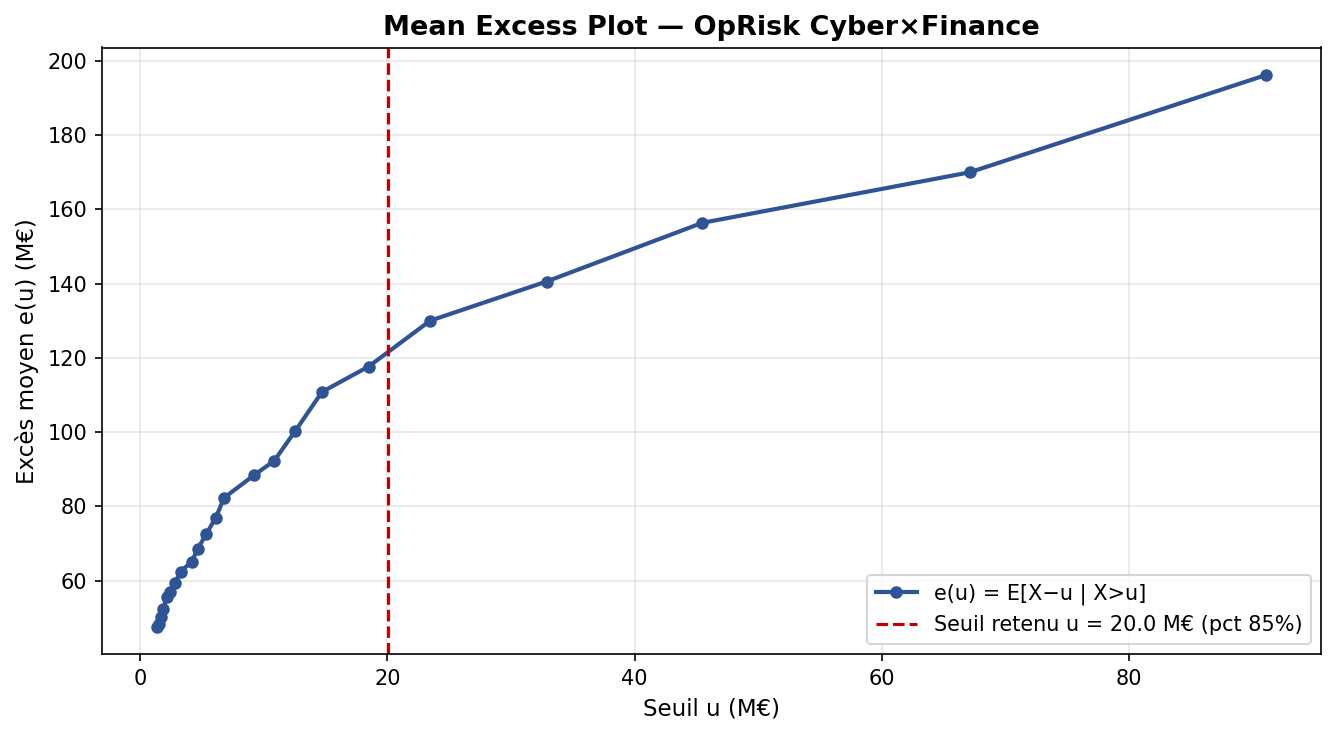
\includegraphics[width=0.85\textwidth]{figures/mean_excess_oprisk.png}
\caption{Mean excess plot sur le périmètre cyber$\times$finance d'OpRisk
Global. La linéarité de $e(u)$ au-delà du seuil retenu $u = 20$~M\euro
(pointillés) confirme le régime de queue lourde justifiant l'ajustement GPD.}
\label{don:fig:mep}
\end{figure}

\paragraph{Calibration GPD et validation croisée.} Au seuil du percentile~85
($u = 20{,}0$~M\euro, 91 excès), la calibration GPD donne :
\[
\hat{\xi} = 0{,}595 \quad (\text{IC}_{90\%}=[0{,}30\,;\,0{,}83]), \qquad
\hat{\sigma} = 58{,}0~\text{M\euro}, \qquad
\qsev_{99{,}5\%}(X) = 663~\text{M\euro}.
\]
Le dernier terme est le quantile de la sévérité d'un sinistre, pas un capital : le
besoin de capital est le quantile de la charge \emph{annuelle agrégée}, obtenu plus loin par
composition avec la fréquence. L'intervalle de confiance bootstrap qui entoure ce quantile est
$[411\,;\,1037]$~M\euro, soit un facteur~2{,}5 entre les bornes, une ampleur qui, à elle seule,
illustre que le SCR ne peut être présenté comme un point.

La comparaison avec la PRC ($\hat{\xi}_{\text{PRC}} = 1{,}03$ contre
$\hat{\xi}_{\text{OpRisk}} = 0{,}595$) ne se lit pas comme une différence de
risque, car les deux indices ne portent pas sur le même objet. La sévérité PRC
n'est pas observée : elle est une puissance du nombre d'enregistrements, de
pente $0{,}76$ en logarithme, et une puissance multiplie l'indice de queue par
son exposant, si bien que $\hat{\xi}_{\text{PRC}}$ décrit la queue des
enregistrements transportée en euros. Le biais de taille d'OpRisk, mesuré faible
au \S\ref{sec:biais-chiffres}, n'en rend pas compte. Les deux sources confirment néanmoins le même régime
qualitatif de queue lourde ($\xi > 0$). Il n'existe donc pas de hiérarchie
\og source primaire\fg{} en sévérité : OpRisk fournit des montants réels, la PRC
un spectre de tailles plus large via la conversion Jacobs : deux
estimations indépendantes et complémentaires, dont l'écart constitue
lui-même une information sur l'incertitude du modèle.

La décomposition par sous-catégorie révèle en outre deux profils de risque
distincts : les pannes (\og Business Disruption\fg{}) sont moins fréquentes
(19~\% des incidents) mais nettement plus coûteuses, avec une médiane cinq
fois supérieure à celle des intrusions (\og Systems Security\fg{}), suggérant que
les multiplicateurs DORA pourraient à terme être différenciés non seulement
en fréquence mais aussi en sévérité, sous réserve de la taille réduite de
l'échantillon \og pannes\fg{} (28 excès), qui rend cette calibration indicative.

%--------------------------------------------------------------

%--------------------------------------------------------------

\section{Portée et limites du dispositif de données}
\label{sec:portee-donnees}

La discipline méthodologique retenue dans ce mémoire consiste à ne jamais
prétendre inférer davantage que ce que les données permettent réellement, ce
qui impose d'expliciter aussi bien les capacités que les limites du dispositif.

\paragraph{Ce que l'on sait faire.} On sait lire une fréquence d'incidents
matériels sur des pertes observées (OpRisk Global), et la moduler entre états de
conformité selon une structure d'attaque citée (Hackmageddon).
On sait calibrer une sévérité de queue lourde par la théorie des valeurs
extrêmes à partir de pertes réellement observées (OpRisk Global), et
confronter cette calibration à une source indépendante pour objectiver
l'incertitude. On sait enfin traiter l'écart entre sources non comme un bruit
à éliminer, mais comme une dimension d'incertitude à part entière, qui
s'ajoute à l'incertitude de paramètre estimée par bootstrap.

\paragraph{Ce que l'on ne sait pas faire.} On ne sait pas mesurer directement
le niveau de conformité DORA d'une entité donnée ; c'est précisément la
raison d'être de l'état de conformité par pilier introduit au
chapitre~\ref{chap:multietats}. On ne sait pas
disposer d'une base d'incidents harmonisée à l'échelle européenne, exhaustive
et non biaisée par la visibilité médiatique. On ne sait pas non plus estimer
avec précision la corrélation entre les différentes briques de perte,
faute d'historique suffisant sur les événements joints ; cette incertitude
est traitée au chapitre~\ref{chap:cascade} par une structure de dépendance explicite plutôt que
par une hypothèse d'indépendance non fondée.

Deux règles du moteur de simulation, le plafond de sévérité propre à la source PRC et la
sévérité nulle sous le seuil, ainsi que la suffisance des trois sources pour un exercice
d'ORSA, sont précisées au \S\ref{sec:ann-sources}.

% SOURCES-SCRIPTS: 05 63

\section{Pourquoi ne pas multiplier les sources}

Des bases
supplémentaires existent (bases commerciales de sinistres cyber assurantiels,
enquêtes sectorielles européennes) et pourraient, en principe, enrichir le
dispositif. Mais chacune porterait ses propres biais de sélection et de
représentativité, sans lever la limite structurelle identifiée plus haut :
l'absence, à ce jour, d'un registre harmonisé et exhaustif à
l'échelle du marché. Multiplier les sources déplacerait la difficulté sans la
résoudre, et complexifierait un dispositif dont les rôles sont aujourd'hui distincts (trois
sources, trois rôles, aucune hiérarchie de \og source primaire\fg{}). L'analyse de sensibilité menée
au chapitre~\ref{chap:resultats} confirme d'ailleurs, \emph{a posteriori}, la pertinence de ce choix :
c'est l'incertitude sur l'indice de queue $\xi$ de la sévérité, estimé sur
les sources déjà mobilisées, qui domine très largement toute autre source
de variation du modèle, multipliers de fréquence et paramètres de dépendance
compris. Approfondir l'exploitation des trois sources retenues (bootstrap,
validation croisée, diagnostics de stabilité) réduit donc l'incertitude du
capital de façon bien plus significative que l'ajout d'une quatrième base de
sinistralité.

%--------------------------------------------------------------

%--------------------------------------------------------------

La structure tirée de Hackmageddon est confrontée au rapport \emph{ENISA Threat Landscape 2025}
\citep{enisa2025}, de méthodologie de collecte distincte, qui confirme la même hiérarchie des
vecteurs d'attaque par leur taux de conversion en intrusion (\S\ref{sec:ann-sources}).

%==============================================================

\begin{cle}
\textbf{Ce que ces données permettent, et ce qu'elles interdisent.} Elles fixent la queue de
sévérité ($\hat\xi = 0{,}595$ sur OpRisk), la fréquence d'entrée et l'accumulation par cause
commune. Elles ne fixent \emph{pas} la direction de la contagion : le
chapitre~\ref{ch:identifiabilite} le montre sur trois sources qui échouent pour des raisons
distinctes, et le
chapitre~\ref{chap:partielle} en tire les conséquences en bornes de capital. Cette frontière
est un résultat produit par le dispositif de données, non une lacune de celui-ci.
\end{cle}

% =====================================================================

% SOURCES-SCRIPTS: 05 62 63
         % Sources, périmètres, retraitements, limites

% =====================================================================
\part{Modélisation}
\label{part:modele}
% =====================================================================
\chapter{Le socle mécaniste : fréquence et sévérité}
\label{chap:socle}

\noindent Ces deux briques (loi de sévérité GPD par pilier, fréquence surdispersée pilotée par
un facteur commun) sont reprises telles quelles : elles alimentent l'agrégation, qui est le
seul élément que la cascade remplace.

% MIGRÉ depuis memoire/main.tex (plages 787-932, 1492-1667).
% Hiérarchie descendue d'un cran, labels préfixés "soc:".
% RELECTURE FAITE (août 2026). Vérifié : aucune phrase de ce chapitre n'annonce la
% copule de Gumbel ni la variable latente comme LE modèle du mémoire ; la copule
% n'apparaît qu'au chapitre 13 comme axe de comparaison de la bande de modèle.
% Deux ambiguïtés de l'ancien modèle ont été levées ici :
%   (a) l'encadré "deux grilles coexistent" articule vecteur d'attaque et pilier ;
%   (b) l'encadré sur lambda_ref dit explicitement que les 341 de la PRC sont une clé
%       de répartition et n'alimentent PAS le moteur (l'entrée est lambda = 21,6).
% La charge systémique empirique a été corrigée sur la sortie réelle du script 08b
% (a = 0,122 [0,054 ; 0,223] ; phi = 2,24), l'ancien "a ~ 0,30 / phi ~ 3" était faux.
%--------------------------------------------------------------

Là où le Théorème Central Limite s'intéresse au comportement asymptotique des sommes de variables aléatoires, la Théorie des Valeurs Extrêmes (EVT) étudie le comportement asymptotique de leurs maxima.

Soit une séquence $(X_1, X_2, \dots, X_n)$ de variables aléatoires indépendantes et identiquement distribuées (i.i.d.) de fonction de répartition $F$, représentant la sévérité des cyberattaques. L'approche initiale de l'EVT, dite des \textit{Block Maxima}, s'intéresse au maximum sur des blocs de taille $n$ (par exemple, le sinistre cyber maximal annuel) :
\begin{equation}
M_n = \max(X_1, X_2, \dots, X_n)
\end{equation}

\section{Les deux théorèmes qui autorisent l'extrapolation de queue}
% HARNAIS-HORS-SECTION: enonces de theoremes. Les nombres y sont des constantes d'enonce
%   (indices de domaine d'attraction, bornes, dates de publication), aucun n'est calcule
%   par le pipeline ; les valeurs empiriques correspondantes sont verifiees dans les
%   sections de calibration et de validation du meme chapitre.

\paragraph{Théorème de Fisher-Tippett-Gnedenko (1928, 1943).} S'il existe des suites de constantes de normalisation $a_n > 0$ et $b_n \in \mathbb{R}$, et une distribution non dégénérée $H$ telles que :
\begin{equation}
\lim_{n \to \infty} \mathbb{P}\left( \frac{M_n - b_n}{a_n} \le x \right) = \lim_{n \to \infty} F^n(a_n x + b_n) = H(x)
\end{equation}
Alors, $H$ appartient nécessairement à la famille des distributions des extrêmes généralisées (GEV - \textit{Generalized Extreme Value}), dont la fonction de répartition s'écrit :
\begin{equation}
H_{\xi}(x) =
\begin{cases}
\exp\left(-\left(1 + \xi x \right)^{-1/\xi}\right) & \text{si } \xi \neq 0 \\
\exp\left(-\exp(-x)\right) & \text{si } \xi = 0
\end{cases}
\end{equation}
définie sur l'ensemble $\{x : 1 + \xi x > 0\}$. Le paramètre $\xi$ (indice de queue) définit trois grands domaines d'attraction :
\begin{itemize}
    \item \textbf{$\xi > 0$ (Loi de Fréchet) :} La distribution présente une queue lourde à décroissance polynomiale. C'est le régime qui décrit les sinistres cyber les plus lourds.
    \item \textbf{$\xi = 0$ (Loi de Gumbel) :} La distribution présente une queue légère à décroissance exponentielle (domaine d'attraction des lois Normale, Lognormale, Gamma).
    \item \textbf{$\xi < 0$ (Loi de Weibull) :} La distribution a un support fini supérieur (queue courte).
\end{itemize}

\noindent On peut énoncer formellement ce résultat fondateur, qui joue pour les maxima le rôle du théorème central limite pour les sommes.

\begin{theorem}[Fisher--Tippett--Gnedenko]\label{soc:th:ftg}
Soit $(X_i)_{i\ge1}$ i.i.d.\ de fonction de répartition $F$ et $M_n=\max(X_1,\dots,X_n)$. S'il existe des suites $a_n>0$, $b_n\in\R$ et une loi non dégénérée $H$ telles que $(M_n-b_n)/a_n \xrightarrow{d} H$, alors $H$ est, à un changement d'échelle et de position près, une loi GEV $H_\xi$. Le signe de $\xi$ détermine le domaine d'attraction : Fréchet ($\xi>0$, queue lourde), Gumbel ($\xi=0$) ou Weibull ($\xi<0$, support borné).
\end{theorem}

\begin{proof}[Éléments]
La loi limite $H$ est nécessairement \emph{max-stable} : pour tout $n$, $H^n(a_nx+b_n)=H(x)$, car $M_{nk}$ est le maximum de $k$ blocs de taille $n$. L'équation fonctionnelle de max-stabilité, résolue via la théorie des fonctions à variation régulière, n'admet (à normalisation près) que la famille à un paramètre $H_\xi$. La correspondance queue de $F$ $\leftrightarrow$ signe de $\xi$ s'obtient en caractérisant les $F$ dont la fonction de survie est à variation régulière d'indice $-1/\xi$ (cas Fréchet). Le détail figure en Annexe~\ref{soc:ann:ftg}.
\end{proof}

%--------------------------------------------------------------

%--------------------------------------------------------------

L'approche \textit{Block Maxima} (GEV) est rigoureuse mais coûteuse en information. En ne
retenant que le maximum de chaque bloc, elle écarte le deuxième plus grand sinistre d'une année
extrême, lequel peut dépasser le maximum d'une année calme. Sur une donnée cyber aussi peu
fournie, ce rejet d'observations fragiliserait l'ajustement.

Pour contourner ce problème, ce mémoire privilégie l'approche \textit{Peaks-Over-Threshold} (POT). Au lieu de ne garder que les maxima, cette méthode exploite toutes les observations excédant un seuil élevé $u$. On s'intéresse alors à la distribution des excès $Y = X - u$.

La fonction de répartition conditionnelle des excès est donnée par :
\begin{equation}
F_u(y) = \mathbb{P}(X - u \le y \mid X > u) = \frac{F(u+y) - F(u)}{1 - F(u)}
\end{equation}

\paragraph{Théorème de Balkema-de Haan-Pickands (1974).} Ce théorème établit le pont mathématique entre la GEV et l'approche POT. Pour une large classe de distributions sous-jacentes $F$ (celles appartenant au domaine d'attraction d'une loi GEV $H_\xi$), il existe une fonction mesurable positive $\sigma(u)$ telle que, lorsque le seuil $u$ tend vers la limite supérieure du support de $F$ ($x_F$), la distribution des excès converge asymptotiquement vers une distribution de Pareto Généralisée (GPD) :
\begin{equation}
\lim_{u \to x_F} \sup_{0 \le y < x_F - u} \left| F_u(y) - G_{\xi, \sigma(u)}(y) \right| = 0
\end{equation}

Où la fonction de répartition de la GPD s'écrit :
\begin{equation}
G_{\xi, \sigma}(y) =
\begin{cases}
1 - \left(1 + \frac{\xi y}{\sigma}\right)^{-1/\xi} & \text{si } \xi \neq 0 \\
1 - \exp\left(-\frac{y}{\sigma}\right) & \text{si } \xi = 0
\end{cases}
\end{equation}
avec $y \ge 0$ si $\xi \ge 0$, et $0 \le y \le -\sigma/\xi$ si $\xi < 0$. Le paramètre de forme $\xi$ de la GPD est strictement le même que celui de la loi GEV correspondante. Dans le contexte du risque cyber, un indice de queue $\xi > 0$ traduit une distribution à queue lourde de type Fréchet, impliquant des moments potentiellement infinis (l'espérance est infinie si $\xi \ge 1$, la variance si $\xi \ge 0.5$). Le résultat s'énonce formellement ainsi.

\begin{theorem}[Pickands--Balkema--de Haan]\label{soc:th:balkema}
Soit $F$ dans le domaine d'attraction d'une GEV $H_\xi$ (Théorème~\ref{soc:th:ftg}). Alors il existe une fonction $\sigma(u)>0$ telle que la loi des excès converge uniformément vers une GPD lorsque le seuil approche la borne supérieure $x_F$ du support :
\begin{equation}
\lim_{u\to x_F}\ \sup_{0\le y< x_F-u}\bigl|F_u(y)-G_{\xi,\sigma(u)}(y)\bigr|=0,
\end{equation}
où $F_u(y)=\Prob(X-u\le y\mid X>u)$ et $G_{\xi,\sigma}$ est la fonction de répartition de la GPD. L'indice de queue $\xi$ est identique à celui de la GEV limite.
\end{theorem}

\begin{proof}[Esquisse]
L'appartenance de $F$ au domaine d'attraction de $H_\xi$ équivaut à une condition de variation régulière sur la fonction de survie $\bar F$. On montre que $\bar F(u+y\,a(u))/\bar F(u)\to(1+\xi y)^{-1/\xi}$ quand $u\to x_F$, pour une fonction d'échelle $a(u)$ adéquate ; ce membre de droite est exactement la fonction de survie GPD. La convergence uniforme découle de la monotonie des fonctions de répartition (théorème de Pólya). Détail et lien avec le Théorème~\ref{soc:th:ftg} en Annexe~\ref{soc:ann:balkema}.
\end{proof}

%--------------------------------------------------------------

%--------------------------------------------------------------

L'estimation de l'indice de queue $\xi$ est un enjeu critique, car une infime variation de ce paramètre modifie massivement le Capital de Solvabilité Requis (SCR). Deux approches principales s'affrontent dans la littérature.

\section{Estimer l'indice de queue, et savoir ce que vaut l'estimation}

% SOURCES-SCRIPTS: 47 63 67

\paragraph{L'estimateur de Hill.}
Pour $\xi > 0$, l'estimateur non paramétrique de Hill (1975) estime l'indice de queue à partir des $k$ plus grandes statistiques d'ordre, sans passer par l'ajustement d'une loi paramétrique. Asymptotiquement convergent et sans biais lorsque la loi appartient au domaine d'attraction de Fréchet, il présente en échantillon fini un biais majeur : si la composante à variation lente de la queue ne converge pas assez vite, $\hat{\xi}_{\text{Hill}}$ devient instable.

\paragraph{Le Maximum de Vraisemblance (MLE).}
Pour pallier le biais de l'estimateur de Hill hors du régime asymptotique strict, ce mémoire privilégie l'estimation par Maximum de Vraisemblance (MLE) sur les excès de la GPD. La log-vraisemblance pour un échantillon de $N_u$ excès $y_i$ au-delà du seuil $u$ s'écrit (pour $\xi \neq 0$) :
\begin{equation}
\ell(\xi, \sigma) = -N_u \ln(\sigma) - \left(1 + \frac{1}{\xi}\right) \sum_{i=1}^{N_u} \ln\left(1 + \frac{\xi y_i}{\sigma}\right)
\label{soc:eq:loglik-gpd}
\end{equation}
La maximisation numérique de cette fonction fournit des estimateurs $(\hat{\xi}_{MLE}, \hat{\sigma}_{MLE})$ qui, bien que nécessitant des méthodes d'optimisation (algorithme de Nelder-Mead), offrent une robustesse supérieure face à la variance d'échantillonnage des bases de sinistres cyber comme OpRisk ou PRC.

\paragraph{Loi asymptotique et information de Fisher.} La qualité d'un intervalle de confiance sur $\xi$ conditionne toute la lecture du capital. Le fondement théorique en est donné ici ; il sert de contrôle indépendant du bootstrap employé au chapitre~\ref{chap:resultats}.

\begin{proposition}[Normalité asymptotique de l'EMV de la GPD]\label{soc:prop:fisher}
Pour $\xi > -\tfrac{1}{2}$, l'estimateur du maximum de vraisemblance $(\hat\xi,\hat\sigma)$ de la GPD est consistant et asymptotiquement normal :
\begin{equation}
\sqrt{N_u}\,\begin{pmatrix}\hat\xi-\xi\\[2pt]\hat\sigma-\sigma\end{pmatrix}
\;\xrightarrow{\;d\;}\;
\mathcal{N}\!\left(\mathbf{0},\; (1+\xi)\begin{pmatrix}1+\xi & -\sigma\\[2pt] -\sigma & 2\sigma^2\end{pmatrix}\right).
\end{equation}
En particulier, la variance asymptotique de l'indice de queue est
$\Var(\hat\xi)\simeq (1+\xi)^2/N_u$.
\end{proposition}

\begin{proof}[Esquisse]
La matrice de covariance limite est l'inverse de l'information de Fisher $\mathcal{I}(\xi,\sigma)$, obtenue en prenant l'espérance de l'opposé de la hessienne de $\ell$. Le détail du calcul de $\mathcal{I}$ (dérivées secondes de \eqref{soc:eq:loglik-gpd} et intégration contre la densité GPD, valide pour $\xi>-\tfrac12$ où l'information est finie) est reporté en Annexe~\ref{soc:ann:fisher}. Le résultat classique remonte à \citet{smith1987}.
\end{proof}

\noindent Appliquée à la calibration OpRisk ($\hat\xi=0{,}595$, $N_u=91$ excès), la Proposition~\ref{soc:prop:fisher} donne un écart-type asymptotique $\widehat{\mathrm{sd}}(\hat\xi)=(1+\hat\xi)/\sqrt{N_u}=0{,}167$, soit un intervalle de confiance à 90\,\% par la delta-méthode de $[0{,}320\,;\,0{,}870]$. Cet intervalle recoupe presque exactement l'intervalle bootstrap $[0{,}304\,;\,0{,}831]$ obtenu indépendamment au \S\ref{soc:sec:severite} : la concordance des deux approches, l'une paramétrique et asymptotique, l'autre par rééchantillonnage, renforce la fiabilité de l'incertitude reportée sur~$\xi$.

\begin{proposition}[Loi asymptotique de l'estimateur de Hill]\label{soc:prop:hill}
Si $F$ est à variation régulière d'indice $-1/\xi$ (domaine de Fréchet), alors pour une suite $k=k(n)\to\infty$ avec $k/n\to0$,
\begin{equation}
\sqrt{k}\,\bigl(\hat\xi_{Hill}(k)-\xi\bigr)\;\xrightarrow{\;d\;}\;\mathcal{N}(0,\;\xi^2).
\end{equation}
\end{proposition}

\noindent L'écart-type $\xi/\sqrt{k}$ décroît en $\sqrt{k}$ : d'où l'arbitrage biais--variance qui gouverne le choix de $k$ dans le \emph{Hill plot}, et qui explique l'instabilité signalée plus haut lorsque $k$ est pris trop grand (contamination par le corps de la loi) ou trop petit (variance explosive). La preuve, fondée sur la représentation de Rényi des espacements exponentiels, est esquissée en Annexe~\ref{soc:ann:hill}.

\paragraph{Quantile de sévérité : formules fermées, et ce qu'elles ne donnent pas.} Le passage des paramètres $(\xi,\sigma)$ au quantile d'\emph{un} sinistre est explicite. Il faut dire tout de suite ce qu'il n'est pas : ce quantile n'est pas un besoin de capital, et l'on n'y accède au capital qu'après agrégation annuelle de la fréquence et de la sévérité, puis propagation dans la cascade (chapitre~\ref{chap:cascade}). Notons $\zeta_u=\Prob(X>u)$ la probabilité de dépassement du seuil. Les formes qui suivent sont
classiques \citep{mcneil2015}.

\begin{proposition}[Quantile et moyenne de queue d'une sévérité GPD]\label{soc:prop:varestvar}
Sous le modèle POT, pour $\alpha$ tel que $\qsev_\alpha(X)>u$ et $\xi\in(0,1)$ :
\begin{align}
\qsev_\alpha(X) &= \boxed{\,u + \frac{\sigma}{\xi}\left[\left(\frac{1-\alpha}{\zeta_u}\right)^{-\xi}-1\right]\,},\label{soc:eq:var-gpd}\\[4pt]
\qbarsev_\alpha(X) = \E[X\mid X>\qsev_\alpha(X)] &= \boxed{\,\frac{\qsev_\alpha(X)}{1-\xi}+\frac{\sigma-\xi u}{1-\xi}\,}.\label{soc:eq:tvar-gpd}
\end{align}
Lorsque $\xi\ge 1$, l'espérance $\E[X]$ est infinie et $\qbarsev_\alpha$ n'est pas définie.
\end{proposition}

\begin{proof}
Pour $x>u$, la propriété POT donne $\Prob(X>x)=\zeta_u\bigl(1+\xi(x-u)/\sigma\bigr)^{-1/\xi}$. En posant ce membre égal à $1-\alpha$ et en inversant, on obtient \eqref{soc:eq:var-gpd}. Pour \eqref{soc:eq:tvar-gpd}, la stabilité de la GPD par franchissement de seuil implique que l'excès au-delà de $\qsev_\alpha(X)$ suit encore une GPD de paramètre $\xi$ et d'échelle $\sigma+\xi(\qsev_\alpha(X)-u)$, d'espérance $\bigl(\sigma+\xi(\qsev_\alpha(X)-u)\bigr)/(1-\xi)$ pour $\xi<1$ ; en ajoutant $\qsev_\alpha(X)$ et en réarrangeant, on retrouve \eqref{soc:eq:tvar-gpd}. La divergence pour $\xi\ge1$ découle de $\E[X]=\int_u^\infty \Prob(X>x)\,\dd x=+\infty$ dès que $1/\xi\le1$. Détail en Annexe~\ref{soc:ann:varestvar}.
\end{proof}

\noindent Numériquement, la calibration OpRisk ($u=20{,}03$, $\sigma=57{,}97$, $\xi=0{,}595$, $\zeta_u=0{,}151$) donne par \eqref{soc:eq:var-gpd} un quantile de sévérité $\qsev_{99{,}5\%}(X)=663{,}0$~M\euro\ et par \eqref{soc:eq:tvar-gpd} une moyenne de queue $\qbarsev_{99{,}5\%}(X)=1\,752{,}4$~M\euro.

\begin{attention}
\textbf{Ces deux nombres ne sont pas des capitaux, et le mémoire ne les compare jamais à un SCR.}
Ils décrivent \emph{un} sinistre. La mesure de capital est $\VaR_{99{,}5\,\%}(L)$, quantile de la
charge \emph{annuelle agrégée}, et elle vaut plusieurs milliers de millions d'euros à l'échelle
sectorielle : l'écart avec les $663$~M\euro\ ci-dessus ne traduit aucune incohérence, il traduit
l'agrégation. À $\lambda\simeq21{,}6$ sinistres matériels par an, atteindre le quantile annuel à
$99{,}5\,\%$ demande un quantile \emph{par sinistre} de l'ordre de $99{,}98\,\%$, bien plus haut
dans la queue. Le pont entre les deux échelles est chiffré au chapitre~\ref{chap:resultats}.
% SOURCES-SCRIPTS: 67
Réserver $\VaR$ et $\TVaR$ à $L$, et $\qsev$ et $\qbarsev$ à
$X$, n'est donc pas une coquetterie de notation : c'est ce qui empêche de lire une différence
d'échelle comme une contradiction.
\end{attention}

\noindent La Proposition~\ref{soc:prop:varestvar} éclaire par ailleurs le contraste entre sources : la calibration PRC affiche $\hat\xi=1{,}033>1$, ce qui place la sévérité en régime d'espérance infinie : la moyenne de queue, et donc tout Expected Shortfall bâti sur elle, y est mathématiquement indéfinie. C'est ce qui justifie \emph{a posteriori} le recours à un plafond de sévérité (capacité de réassurance) pour rendre le capital PRC calculable, et c'est aussi le premier argument contre l'usage d'une mesure de queue comme \emph{niveau de couverture} : sur l'une des deux sources, cette mesure n'existe pas.

%--------------------------------------------------------------


%--------------------------------------------------------------

\begin{attention}
\textbf{Deux grilles coexistent dans ce chapitre, et elles ne sont pas concurrentes.} La
première décrit \emph{comment} un incident entre : par vecteur d'attaque (hameçonnage,
exploitation de vulnérabilité, chaîne d'approvisionnement). La seconde décrit \emph{quel
contrôle} a cédé : par pilier DORA. Un vecteur n'est pas un pilier, et il serait faux
de les apparier terme à terme. Leur articulation est de type \emph{entrée puis propagation} :
le vecteur gouverne l'amorce, c'est-à-dire la fréquence d'arrivée d'un sinistre et le
pilier sur lequel il tombe ; la cascade du chapitre~\ref{chap:cascade} gouverne ensuite la
\emph{propagation} entre piliers. Le présent chapitre calibre donc l'amorce et rien d'autre.
La grille par vecteur ne réapparaît plus après lui, et aucun résultat de capital ne dépend de
son appariement à un pilier.
\end{attention}

\section{La brique de fréquence}

\paragraph{Décomposition par vecteur d'attaque.} Une fréquence de référence
$\lambda_{ref}$, lue sur le périmètre financier de la base PRC
($\lambda_{ref} = 341$ notifications/an), est décomposée en
% SOURCES-SCRIPTS: 62
sous-fréquences par vecteur d'attaque,
pondérées par la structure observée dans la base Hackmageddon :
\begin{equation}
\lambda_{ref} = \sum_{v} \lambda_v,
\qquad
\lambda_v = \lambda_{ref} \times \pi_v,
\end{equation}
où $\pi_v$ est la part du vecteur $v$ dans la structure Hackmageddon
(38{,}8~\% phishing, 33{,}8~\% exploitation de vulnérabilités, 15{,}8~\%
supply chain, 6{,}3~\% identifiants compromis, 5{,}3~\% autres). Cette
décomposition transforme un constat structurel en levier de modélisation :
un défaut de conformité sur une exigence donnée n'agit que sur la
sous-fréquence du vecteur qu'elle est censée mitiger, pas sur l'ensemble de
$\lambda_{ref}$.

\begin{attention}
\textbf{$\lambda_{ref}$ est une clé de répartition, pas le niveau du modèle.} Les $341$ de la
PRC comptent des \emph{notifications de violation de données} déclarées par les organisations
financières de la base, sur un périmètre américain et sans seuil de matérialité. Le périmètre
importe : la base entière en compte $2\,150$ par an, six fois plus, et confondre les deux
rendrait le nombre incompréhensible à qui le recalcule. Ce nombre sert exclusivement à
répartir la sinistralité entre
vecteurs, c'est-à-dire à fixer les $\pi_v$ et à faire jouer les multiplicateurs de conformité.
\textbf{Il n'alimente pas le moteur de cascade.} L'entrée du moteur est la fréquence
d'incidents \textsc{tic} \emph{matériels} lue sur OpRisk, $\lambda \simeq 21{,}6$ par an au
niveau du secteur financier mondial, dont la table du chapitre~\ref{chap:donnees} donne les
trois échelles de lecture. Tout niveau de capital du chapitre~\ref{chap:resultats} repose sur
$\lambda$, jamais sur $\lambda_{ref}$.
\end{attention}

\paragraph{Choix de la loi binomiale négative.} La fréquence agrégée
$\lambda_{S_x} = \sum_v \lambda_{ref}\,\pi_v\, m_{v,S_x}$ obtenue sous un
scénario $S_x$ n'est pas simulée par une loi de Poisson, mais par une loi
binomiale négative, pour tenir compte de la sur-dispersion observée dans les
données ($\sigma^2/\mu > 1$). Le facteur de sur-dispersion
$\phi = \sigma^2/\mu = 9{,}2$ est traité comme une propriété structurelle de
la sinistralité, supposée indépendante du niveau de fréquence : c'est donc
$\phi$ qui est maintenu constant d'un scénario à l'autre, et non le
paramètre $r$ de la binomiale négative, qui est au contraire recalculé sous
chaque scénario :
\begin{equation}
r_{S_x} = \frac{\lambda_{S_x}}{\phi - 1},
\qquad
p_{S_x} = \frac{r_{S_x}}{r_{S_x} + \lambda_{S_x}}.
\end{equation}
Augmenter $\lambda$ via les multiplicateurs DORA déplace ainsi la fréquence
moyenne tout en préservant la \emph{forme} de sur-dispersion de la
sinistralité, hypothèse de modélisation explicite, dont la limite est
que le comportement de la sur-dispersion en régime de forte dégradation
n'est pas lui-même observé, faute d'historique de crise DORA.

\paragraph{Réconciliation des quatre mesures de surdispersion, et effet sur le capital.}
Avant les trois mesures de forme, un mot sur celle que l'on observe directement, car un lecteur
qui parcourt ce chapitre rencontre \emph{quatre} nombres de surdispersion et pourrait les croire
en concurrence. Ils ne le sont pas, ils vivent à des échelles différentes, et
l'indice de dispersion n'est pas invariant d'échelle : pour un mélange de Poisson il
vaut $1+\lambda/r$, donc il croît avec le niveau de fréquence auquel on le lit. Sur les
$14\,944$ cellules firme-année du panel, où la fréquence moyenne est de l'ordre de quatre
centièmes d'incident par cellule, on mesure $\Var/\E=1{,}19$. Sur la série annuelle sectorielle
détendancée, où $\lambda$ vaut $21{,}6$, on mesure $2{,}24$. Le moteur, lui, retient $9{,}20$,
qui est un choix de prudence posé et non une mesure. Une échelle de lecture, une
agrégation de cellules corrélées, puis une marge prudentielle assumée : les trois écarts
s'expliquent l'un après l'autre, et aucun ne contredit les autres.
Le modèle porte, à trois échelles distinctes, trois mesures de surdispersion qu'il faut
réconcilier pour ne pas les confondre : la forme du mélange Gamma au niveau firme-année
($r=0{,}63$), la charge systémique commune ($a=0{,}60$, mélange lognormal du
chapitre~\ref{chap:multietats}) et le facteur $\varphi=9{,}20$ ci-dessus (mélange Gamma
agrégé, c'est-à-dire la binomiale négative). Un mélange de Poisson a pour indice de dispersion
$\Var/\E$ égal à $1+\lambda/r=\varphi$ (mélange Gamma) ou $1+\lambda(e^{a^2}-1)$ (mélange
lognormal) ; les deux décrivent \emph{la même} surdispersion agrégée dès lors que
$a=\sqrt{\ln\!\bigl(1+(\varphi-1)/\lambda\bigr)}$. À l'échelle du moteur ($\lambda\simeq 21{,}6$
entrées par an), $\varphi=9{,}20$ correspond à $a=0{,}57$, soit à cinq pour cent de la valeur
$0{,}60$ posée par ailleurs : les deux calages agrégés coïncident, le $r=0{,}63$ firme vivant à
une échelle firme-année non comparable directement.

Trois enseignements suivent (figure~\ref{soc:fig:nb}). D'abord, à variance égale la queue
dépend encore de la loi de mélange : le quantile $99{,}5\,\%$ du nombre annuel vaut $74$
(mélange Gamma) contre $82$ (lognormal), soit $+11\,\%$ : appairer la variance n'appaire pas
la queue. Ensuite, le choix de la loi de comptage déplace la VaR mais \emph{non} la moyenne
(l'espérance $\E[N]=\lambda$ est fixe pour les trois lois) : passer du Poisson à la binomiale
négative posée relève le SCR de $+9\,\%$ seulement, la queue restant portée au $99{,}5\,\%$ par
la perte unique dominante ($\xi\simeq 0{,}60$). Enfin, calée sur la série cyber$\times$finance
détrendée, le rapport $\Var/\E$ brut confondant la croissance tendancielle avec le choc
commun, la dispersion de Pearson résiduelle vaut $\varphi=2{,}24$
(IC~$95\,\%$ $[1{,}24\,;5{,}18]$, dix-huit points seulement), soit une charge empirique
$a=0{,}122$ (IC~$95\,\%$ $[0{,}054\,;0{,}223]$). La valeur posée $a=0{,}60$ dépasse donc la
\emph{borne haute} de cet intervalle, et le $\varphi=9{,}20$ retenu au niveau du moteur
dépasse de loin le $2{,}24$ mesuré : l'un comme l'autre sont un choix de prudence sur
la queue de fréquence, non une calibration, à assumer comme tel. La conclusion
\og{}le calage posé est conservateur\fg{} résiste ainsi à l'incertitude d'estimation, ce qui
est la seule chose que dix-huit points autorisent à affirmer.
% SOURCES-SCRIPTS: 47 08b 67 41

\paragraph{La dynamique du facteur systémique.} Le facteur commun $Y_{j,t}$ est posé centré
et réduit. Sa dynamique, écrite au \S\ref{sec:dynamique-Y}, superpose un bruit de fond
brownien et une composante de sauts pour les campagnes de masse. Elle ne déplace aucune
probabilité marginale, donc aucun capital publié, et n'agit que sur la dépendance de queue ; la
forme retenue est la forme à renouvellement, sans mémoire d'un exercice à l'autre.

\begin{figure}[htbp]\centering
\figover{N2_simulation_nb.png}
\caption{La loi de comptage négative binomiale, simulée et réconciliée. (a)~à moyenne égale,
la queue du nombre annuel diffère selon la loi de mélange. (b)~la charge lognormale $a$ et le
facteur $\varphi$ tracent la même surdispersion agrégée ; les deux valeurs posées quasi
coïncident. (c)~le comptage déplace la VaR, pas la moyenne.}
% SOURCES-SCRIPTS: 41
\label{soc:fig:nb}
\end{figure}

\paragraph{De la fréquence par scénario à la fréquence par entité.} Le choix
d'un scénario $S_x \in \{S_0, S_1, S_2\}$ reste, par construction, discret et
appliqué uniformément à l'ensemble du marché. L'état de conformité continu
$C^\star_j$ du chapitre~\ref{chap:multietats} permet de dépasser cette
limite, en substituant à ce choix discret une interpolation continue des multiplicateurs
$m_v$ le long de la latente de conformité,
où $\bar{m}_v^{S_2}$ est le centre de l'intervalle de multiplicateur sourcé
en scénario $S_2$. Une entité au profil de conformité mature conserve ainsi
une fréquence proche de $S_0$ même en cas de choc systémique $Y$
défavorable, tandis qu'une entité en retard de conformité peut, sous un
$\rho_i$ élevé, dépasser le multiplicateur $S_2$ dès l'environnement normal.

%--------------------------------------------------------------

%--------------------------------------------------------------

\section{La brique de sévérité, calibrée sur OpRisk}
\label{soc:sec:severite}

% SOURCES-SCRIPTS: 07 47 63 67

\paragraph{Choix de la loi de Pareto généralisée.} La sévérité des sinistres
cyber présente une signature de queue lourde documentée au chapitre~\ref{chap:donnees} : sur
OpRisk Global, sur la population de la fréquence et de la descente d'échelle, les $10\,\%$ d'incidents les plus
graves concentrent $92{,}3\,\%$
de la perte totale. Cette concentration extrême justifie le recours à la
théorie des valeurs extrêmes, et plus précisément à une modélisation de la
queue de distribution par une loi de Pareto généralisée (GPD) au-delà d'un
seuil $u$, selon l'approche \emph{peaks-over-threshold}.

\paragraph{Calibration OpRisk.} Au seuil du percentile~85
($u = 20{,}0$~M\euro, 91 excès), la calibration donne :
\begin{equation}
\hat{\xi}_{\text{OpRisk}} = 0{,}595 \quad (\text{IC}_{90\%}=[0{,}30\,;\,0{,}83]),
\qquad
\hat{\sigma}_{\text{OpRisk}} = 58{,}0~\text{M\euro},
\qquad
\qsev_{99{,}5\%}(X) = 663~\text{M\euro}.
\end{equation}
Le dernier terme est un quantile de sévérité, c'est-à-dire le montant d'\emph{un}
sinistre, et non un besoin de capital. L'intervalle de confiance bootstrap qui l'entoure,
$[411\,;\,1037]$~M\euro, matérialise à lui seul un facteur~2{,}5 entre les bornes, uniquement
imputable à l'incertitude de paramètre.

\paragraph{Ce que le seuil doit aux diagnostics, et ce qu'il ne leur doit pas.} Le choix de $u$
s'appuie sur deux diagnostics, à condition de ne leur faire dire ni plus ni autre chose que ce
qu'ils disent. Le \emph{diagnostic GPD} (figure~\ref{soc:fig:diagnostic-gpd}) établit un point,
et un seul : le seuil retenu se situe à la frontière où le paramètre de forme quitte la zone
instable ($\xi \geq 1$, où l'espérance n'existe pas) pour un régime de moments finis, tout en
conservant assez d'excès pour estimer ($n = 91 > 30$). C'est un argument de voisinage,
et il ne s'étend pas à toute la plage : en portant le seuil au percentile $90$ puis au percentile
$95$ des données, l'indice descend de $0{,}60$ à $0{,}53$ puis $0{,}38$. Écrire que
$\hat\xi$ est \emph{stable} quand on fait varier le seuil serait donc inexact ; ce qui est
stable, c'est son voisinage, où il ne bouge que de $0{,}5\,\%$. Cette décroissance est mesurée
au \S\ref{soc:sec:validation}, avec ce qu'elle change et ce qu'elle ne change pas. Quant au
\emph{Hill plot} (figure~\ref{soc:fig:hill-ic}), il ne corrobore pas ce niveau par sa valeur,
qui en vaut plus du double : la section suivante établit que cet écart est exactement ce qu'un
$\xi$ de $0{,}60$ produit en échantillon fini, ce qui en fait une corroboration d'un autre
genre, et plus forte que la lecture d'un plateau.

\begin{figure}[htbp]
\centering
\figover{figures/diagnostic_gpd_oprisk.png}
\caption{Diagnostic GPD sur le périmètre cyber$\times$finance d'OpRisk.
\textit{Gauche} : $\hat{\xi}$ en fonction du seuil $u$ ; le paramètre passe sous
$\xi = 1$ (espérance finie) avant le seuil retenu $u = 20$~M\euro. La plage tracée
s'arrête en deçà des seuils les plus élevés du balayage en percentiles, où l'indice
descend plus bas : cette figure atteste le \emph{voisinage} du seuil, non une stabilité
d'ensemble, et la décroissance complète est mesurée au \S\ref{soc:sec:validation}.
\textit{Droite} : le nombre d'excès correspondant ($n = 91$) demeure au-dessus du
minimum de $30$ requis pour une estimation robuste.}
\label{soc:fig:diagnostic-gpd}
\end{figure}

\section{Hill contre maximum de vraisemblance : deux estimateurs confrontés}

% SOURCES-SCRIPTS: 47 63 67

L'estimateur de Hill \citep{Hill1975}, appliqué au même périmètre, ne corrobore pas l'indice de
queue par sa valeur : au seuil retenu ($k=86$) il vaut $1{,}32$, soit $120{,}8\,\%$ au-dessus du
maximum de vraisemblance. L'écart est pourtant exactement ce qu'un indice de $0{,}595$ produit en
échantillon fini : sur $2\,000$ échantillons simulés sous le modèle publié, les six valeurs
observées de Hill tombent dans l'intervalle simulé à $90\,\%$. Hill croît en outre avec $k$ quand
le balayage de seuil fait décroître $\hat\xi$, ce qui serait inversé si la queue valait $1{,}32$.
La calibration sur la PRC donne $\hat\xi = 1{,}03$, un indice qui ne porte pas sur le même
objet, la sévérité PRC étant une puissance du nombre d'enregistrements (\S\ref{sec:oprisk}). La
définition de l'estimateur, la table des simulations, le tracé et la validation croisée sont au
\S\ref{sec:ann-hill}.

\section{Validation et adéquation du socle}
\label{soc:sec:validation}

Avant d'agréger, on vérifie que les deux lois posées s'ajustent réellement aux données, faute
de quoi tout le reste serait bâti sur du sable (figure~\ref{soc:fig:validation}).

\textbf{Sévérité.} La GPD passe les diagnostics sans réserve. Les tracés quantile-quantile et
probabilité-probabilité s'alignent sur la diagonale ; la vie résiduelle moyenne est linéaire
au-delà du seuil, ce qui est la signature même d'une queue GPD et justifie le choix de $u$ ;
et $\hat\xi$ est stable dans le \emph{voisinage} du seuil retenu, à $0{,}5\,\%$ près jusqu'au
percentile $85$ des données courantes. Il ne l'est pas sur toute la plage :
en remontant le seuil du percentile $85$ au percentile $95$, l'indice décroît de $0{,}60$ à
$0{,}38$, six seuils comptant chacun au moins trente excès. Cette décroissance reste
\emph{entièrement} dans l'intervalle de confiance à $90\,\%$ déjà publié pour $\xi$,
$[0{,}30\,;0{,}83]$ : la sensibilité au seuil ne crée donc pas d'incertitude nouvelle, elle se
lit dans celle qui est déjà déclarée. En descendant au contraire sous le seuil retenu, $\hat\xi$
remonte jusqu'à $0{,}98$ et sort de cet intervalle par le haut, ce qui est le biais de seuil
attendu lorsqu'on ajuste une loi de queue à des pertes qui n'y appartiennent pas encore, et ce
qui justifie de ne pas descendre plus bas. Les tests formels
ne rejettent pas l'ajustement, avec une $p$-value obtenue par bootstrap paramétrique
les valeurs critiques tabulées ne valant pas lorsque les paramètres sont estimés :
Anderson-Darling $p=0{,}96$, Kolmogorov-Smirnov $p=0{,}89$. Ces deux tests portent sur la
\emph{famille} GPD, paramètres réajustés à chaque tirage. On teste séparément le couple
$(\hat\xi,\hat\sigma)$ \emph{effectivement publié}, paramètres imposés, seule façon d'attester
le chiffre plutôt que le choix de loi : Anderson-Darling $p=0{,}99$, Kolmogorov-Smirnov
$p=0{,}89$, sans rejet non plus. Le seuil retenu ne porte pas la conclusion : au percentile
$85$ des données plutôt qu'au seuil publié, $\hat\xi$ ne bouge que de $0{,}5\,\%$. Enfin,
la couverture réelle
de l'intervalle de confiance à $90\,\%$ de $\xi$, mesurée par simulation à $n$ fini, vaut
$86\,\%$. Le mot juste n'est pas \og{}proche du nominal\fg{} : un intervalle annoncé à
$90\,\%$ qui n'en couvre que $86$ est trop étroit, donc l'incertitude reportée sur
$\xi$ est sous-estimée et non l'inverse. Sous l'approximation normale, atteindre le nominal
demanderait d'élargir la demi-largeur d'environ $10\,\%$. L'écart est petit, mais son sens
compte, et il rejoint celui du taux de dépassement gelé au \S\ref{sec:pu-coherence} ainsi que
celui de la dérive d'échelle mesurée au \S\ref{soc:sec:backtest} : les trois seuls défauts
d'estimation du mémoire vont du même côté, celui de la sous-estimation, quand tous ses choix
\emph{posés} vont du côté prudent. C'est aussi ce qui justifie de rapporter les
intervalles bootstrap plutôt que les asymptotiques.

\textbf{Fréquence.} Sur les $14\,944$ cellules firme-année du panel financier, la binomiale
négative domine le Poisson sans ambiguïté : le test du rapport de vraisemblance donne
$p\approx 10^{-30}$. La surdispersion ($\Var/\E=1{,}19$) est donc un \emph{fait}, non un
artefact, et la NB épouse la queue des comptes là où le Poisson s'effondre.

\begin{figure}[htbp]\centering
\figover{J3_validation_adequation.png}
\caption{Validation du socle. (a-b) QQ-plot et PP-plot de la sévérité contre la GPD
ajustée. (c) vie résiduelle moyenne, linéaire au-delà de $u$. (d) stabilité
de $\hat\xi$ au seuil. (e) test d'Anderson-Darling, loi nulle par bootstrap
paramétrique et statistique observée ($p=0{,}96$). (f) adéquation de la fréquence :
la NB colle aux comptes firme-année, le Poisson rate la queue.}
% SOURCES-SCRIPTS: 47 93
\label{soc:fig:validation}
\end{figure}

\paragraph{Le seuil est une règle, pas un choix.} Une règle de stabilité écrite, appliquée à dix
percentiles candidats, retient $19{,}87$~M\euro{} contre $20{,}03$ publiés, avec un quantile
identique, et ce seuil est aussi le mieux ajusté du balayage. La règle la plus permissive
descendrait à $12{,}88$~M\euro{} et donnerait un quantile de sévérité supérieur de $16{,}0\,\%$ :
le seuil publié n'est pas celui qui maximise le chiffre du mémoire. Les deux règles et l'absence
de compromis entre biais et variance sur cette grandeur sont au \S\ref{sec:ann-seuil}.

\begin{cle}
\textbf{Ce que la validation établit, et ce qu'elle n'établit pas.} Les tests portent sur la
\emph{forme} des lois, pas sur le \emph{niveau} du capital : ils confirment que la GPD et la
NB sont les bons objets, mais laissent entière l'incertitude sur $\xi$ et donc sur la VaR (la
bande du chapitre~\ref{chap:resultats}). Adéquation n'est pas certitude : c'est précisément
pourquoi le SCR se lit en intervalle, jamais en point.
\end{cle}

%--------------------------------------------------------------

\section{Le socle hors échantillon : un backtest à origine glissante}
\label{soc:sec:backtest}

Les diagnostics qui précèdent partagent une limite, et elle est de principe plutôt que de
degré : ils interrogent l'ajustement sur les données mêmes qui l'ont produit. Un test
d'adéquation demande si une loi décrit son échantillon, jamais si elle prédit une période
qu'elle n'a pas vue. C'est pourtant la seconde question qu'un lecteur adresse à un modèle de
capital, et cette section y répond.

Le protocole est celui de l'origine glissante. Pour chaque année d'origine, les deux lois sont
ajustées sur les seules observations antérieures, la seule année suivante est notée, puis
l'origine avance d'un an. La fenêtre retenue va de $2004$ à $2025$, soit $539$ incidents, ce qui
donne douze années notées hors échantillon. Deux précautions en conditionnent la lecture. La
fenêtre est choisie sur la donnée et non par commodité : avant $2004$ la base porte de un à neuf
incidents par an contre treize à trente-neuf ensuite, et l'année $2026$ n'en porte que cinq, si
bien qu'une fenêtre plus large fabriquerait un faux régime calme au début et un faux
effondrement à la fin. Et le seuil est ré-estimé sur chaque échantillon d'apprentissage
par la règle du percentile $85$, plutôt que lu dans la calibration figée : un seuil calculé sur
toute la période ferait passer l'information de test dans l'apprentissage, et le test cesserait
de mesurer quoi que ce soit.

\paragraph{Les résultats.} La loi de fréquence est validée : un intervalle de prévision annoncé à
$90\,\%$ en couvre $91{,}7\,\%$ sous la binomiale négative contre $75{,}0\,\%$ sous le Poisson,
et le log-score, qui pénalise la largeur, désigne le même gagnant. La forme de la queue survit au
test de probabilité intégrale ($p=0{,}4087$). Les quantiles de sévérité sont en revanche dépassés
trois fois trop souvent, parce que l'échelle dérive : $4{,}00\,\%$ par an dans la queue, dont la
moitié d'inflation monétaire, les montants de la base étant nominaux, soit au moins
$+24{,}7\,\%$ sur le quantile de sévérité. Cette dérive ne gonfle pas la thèse : le facteur entre
états passe de $3{,}344$ à $3{,}124$ sous la sévérité dérivée, et l'écart en euros ne bouge que
de $-1{,}9\,\%$, par compensation entre forme et échelle. Sur la charge annuelle agrégée le
verdict est négatif, pour la même cause, le désalignement n'apparaissant que sur les dernières
années notées. L'indépendance entre fréquence et sévérité tient sur les excès. Le détail de ces
tests est au \S\ref{sec:ann-backtest}.
% SOURCES-SCRIPTS: 89 90 91 102

\begin{attention}
\textbf{Ce que ce dispositif ne peut pas tester, dit en années plutôt qu'en précaution de style.}
Détecter un taux de dépassement \emph{double} du nominal avec une puissance de $80\,\%$
demanderait $1\,811$ années au niveau de $99{,}5\,\%$, $905$ à $99\,\%$, et $78$ même à
$90\,\%$. Le quantile qui porte le capital n'est donc backtestable sur aucun historique
de risque opérationnel existant, et sur douze années le test ne renseigne que le centre et le
corps de la loi de l'agrégat. Le niveau de capital reste adossé à l'ajustement paramétrique,
dont la queue est corroborée par trois chemins indépendants et bornée par l'intervalle de
$\xi$ ; aucun de ces chemins n'est un backtest du quantile, et le présenter comme tel serait
faux. Un backtest qui ne déclare pas sa puissance laisse croire qu'une absence de rejet vaut
validation.
\end{attention}

\begin{cle}
\textbf{Ce que le backtest établit, et il y a un seul défaut derrière trois symptômes.} La loi de
fréquence est validée hors échantillon, sur deux critères dont un que la largeur n'achète pas. La
forme de la queue survit au test de probabilité intégrale. L'indépendance entre fréquence et
sévérité tient sur la population que le modèle tire. Un seul mécanisme est en défaut,
l'échelle de la sévérité, qui dérive de $4{,}00\,\%$ par an dans la queue, et les trois symptômes
qui restent en découlent : les quantiles de sévérité dépassés trois fois trop souvent, la charge
agrégée rejetée, et un quantile publié anti-conservateur d'au moins $24{,}7\,\%$. La valeur reste
gelée et l'écart est inscrit au registre des limites (\S\ref{sec:pu-coherence}), du même
traitement que le taux de dépassement. Sur la thèse, la formule à retenir est
l'invariance d'échelle et non l'invariance à la dérive : le facteur entre états ne bouge pas
d'une variation d'échelle, mais il baisse de $6{,}6\,\%$ sous la sévérité dérivée, dont la forme
est plus légère.
% SOURCES-SCRIPTS: 89 90 91
\end{cle}

%--------------------------------------------------------------

% =====================================================================
         % Fréquence et sévérité : théorie et calibration
\chapter{La cascade dirigée}
\label{chap:cascade}

\begin{cle}
\textbf{Idée directrice.} La dépendance entre les cinq piliers n'est pas ajoutée après coup par
une copule : elle est \emph{produite} par la propagation d'un incident le long d'une matrice
d'influence dirigée. La cascade est ainsi la vue structurelle (bottom-up) de la
dépendance, en regard de la vue par copule (top-down). Le fil du
chapitre part du Vasicek à un facteur, l'ouvre en deux temps (systémique par pilier, puis
propagation dirigée), et remplace le seuil de défaut du crédit par un seuil ancré sur la barre
de matérialité du règlement.
\end{cle}

\section{Le point de départ : le Vasicek à un facteur et ses limites}

Le modèle structurel de Merton-Vasicek associe à chaque entité une variable latente. On retient
la convention où $X$ mesure le stress et non la santé (un $X$ élevé est une mauvaise
nouvelle), de sorte qu'une contagion positive encode bien une contamination :
\begin{equation}
X_i \;=\; \sqrt{\rho}\;Y \;+\; \sqrt{1-\rho}\;\varepsilon_i, \qquad \mathrm{Var}(X_i)=1,
\end{equation}
où $Y\sim\mathcal N(0,1)$ est le facteur systémique commun, $\varepsilon_i\sim\mathcal N(0,1)$ le
choc idiosyncratique, et $\rho\in[0,1]$ la part du systémique, commune à toutes les entités.
L'incident survient lorsque le stress franchit un seuil, $D_i=\mathbf 1\{X_i\ge K_i\}$, avec dans
le modèle classique $K_i=\Phi^{-1}(1-\mathrm{PD}_i)$.

\begin{attention}
\textbf{Deux hypothèses de ce modèle sont fausses pour le cyber sous DORA.} D'abord, la
dépendance y est symétrique (un seul $Y$, un seul $\rho$) : le modèle ne peut pas dire
\og P1 entraîne P2 plus que l'inverse\fg{}, alors que les données d'expert mobilisées ici
sont dirigées à $81\,\%$. Ensuite, le seuil $\Phi^{-1}(\mathrm{PD})$ suppose une PD stable, mesurable et
une valeur de firme sous-jacente, dont rien n'existe en cyber. Les deux généralisations qui
suivent lèvent ces deux limites.
\end{attention}

% SOURCES-SCRIPTS: 01 03

\section{Généralisation A : la structure systémique dépend du pilier}

On indexe désormais par entité~$i$ et pilier~$j\in\{1,\dots,5\}$, et l'on remplace le facteur
unique par un facteur systémique par pilier $Y_j$ et une sensibilité propre
$\rho_{ij}$ :
\begin{equation}
X_{ij} \;=\; \sqrt{\rho_{ij}}\;Y_j \;+\; \sqrt{1-\rho_{ij}}\;\varepsilon_{ij}.
\end{equation}
Chaque pilier a sa \og météo systémique\fg{} propre (l'état de la menace sur la chaîne
d'approvisionnement pour P4, l'état réglementaire pour P1), et les $Y_j$ sont corrélés entre eux
par une matrice $\Sigma_Y$ : c'est là que vivent proprement les dépendances croisées, au niveau
systémique. Sur des données cyber rares, on ne calibre pas un $\rho_{ij}$ par entité (environ
$5N$ paramètres, non identifiable) : on retient le compromis hiérarchique
$\rho_{ij}=\rho_j+u_{ij}$, où la sensibilité de chaque entité gravite autour de la moyenne de
son pilier $\rho_j$ (pooling partiel).

\begin{cle}
\textbf{La partie A n'est pas une contribution.} Le Merton-Vasicek multifacteur à
matrice de corrélation générale est celui de \citet{Li2000}, employé tel quel en risque de
crédit de portefeuille. La contribution propre ne commence qu'en partie~B, avec
la contagion dirigée. Le revendiquer clairement évite de se voir opposer une
littérature qu'on aurait ignorée.
\end{cle}

\section{Généralisation B : la propagation dirigée}

\begin{cle}
\textbf{Convention d'indices, à fixer une fois pour toutes.} Dans tout le mémoire,
\[
  \boxed{\;W_{jk}\;=\;\text{propension du pilier } j \text{ (source) à entraîner la
  défaillance du pilier } k \text{ (cible).}\;}
\]
La ligne $j$ décrit donc ce que $j$ \emph{émet}, et la colonne $k$ ce que $k$
\emph{reçoit}. C'est la convention du graphe d'arêtes vivantes (définition~\ref{def:cascade} :
l'arc $j\to k$ existe si $B_{jk}=1$) et celle de toutes les implémentations. Elle donne son sens
à la somme de ligne $s_j$, qui mesure l'émission du pilier $j$, et à la revendication
centrale \og{}P1 émet fort et reçoit peu\fg{} : P1 a la plus grande somme de ligne ($2{,}6$) et
une somme de colonne trois fois inférieure à celle de P2. Toute lecture inverse rendrait cette
revendication fausse.
\end{cle}

Pour encoder l'asymétrie, on ajoute un terme de réseau dirigé : le stress de $j$ subit celui des
autres piliers de la même entité, pondéré par une matrice asymétrique $W$. En respectant
la convention ci-dessus, la source est le premier indice, donc le stress \emph{reçu} par $j$
somme les colonnes :
\begin{equation}
X_{ij} \;=\; \underbrace{\sum_{k\neq j} W_{kj}\,X_{ik}}_{\text{contagion dirigée, } k \to j}
   \;+\; \sqrt{\rho_{ij}}\,Y_j \;+\; \sqrt{1-\rho_{ij}}\,\varepsilon_{ij},
\end{equation}
d'où, en forme matricielle sur les cinq piliers, la forme réduite
$\mathbf X_i=(I-W^{\top})^{-1}(\text{systémique}+\text{idio})$, \emph{sous réserve} que
$\rho(W)<1$, le rayon spectral étant invariant par transposition. Si
$W=0$ on retombe sur la partie~A, et avec un seul facteur sur le Vasicek standard :
l'emboîtement est propre.

\begin{figure}[htbp]\centering
\figover{H1_reseau_W.png}
\caption{Structure dirigée de $W$ sur les cinq piliers (P1 émet fort et reçoit peu) et
propagation d'un choc sur un sous-réseau.}
\end{figure}

% SOURCES-SCRIPTS: 29

\section{La normalisation de Leontief : une stabilité garantie}

\begin{attention}
\textbf{Brancher la matrice d'expert TRANS telle quelle est une erreur de catégorie.}
$(I-W)^{-1}$ ne représente une cascade que si la série $I+W+W^2+\cdots$ converge, soit
$\rho(W)<1$. Or $\rho(\mathrm{TRANS})=1{,}461>1$, et $(I-\mathrm{TRANS})^{-1}$ contient
21 entrées négatives sur 25 : un choc positif produirait un stress négatif ailleurs.
TRANS n'a jamais été une matrice de parts.
\end{attention}

La discipline vient du modèle entrées-sorties de Leontief, dont l'inverse
$B=(I-A)^{-1}=\sum_{k\ge0}A^k$ n'explose jamais parce que $A$ est une matrice de parts :
les colonnes somment à moins de un, la différence étant la valeur ajoutée, strictement positive.
On applique la même règle en lisant la ligne $j$ de $W$ comme les parts du stress que $j$
\emph{émet} vers les autres piliers :
\begin{equation}
\label{eq:norm}
\boxed{\;W \;=\; g \cdot \frac{\mathrm{TRANS}}{\max_j \sum_k \mathrm{TRANS}_{jk}}\;,
\qquad g \in (0,\,1]\;}
\end{equation}
où $g$ est la part de contagion du pilier le plus exposé. La contrainte $g\le1$ n'est pas ad
hoc : $W$ est positive et chaque ligne somme à au plus $g$, donc par Perron-Frobenius (le strict
analogue de la valeur ajoutée positive de Leontief)
\begin{equation}
\rho(W)\;\le\;\max_j\sum_k W_{jk}\;\le\;g\;<\;1,
\end{equation}
et $(I-W)^{-1}$ existe. La stabilité est donc garantie par la normalisation, sur tout
le domaine admissible, et non supposée. Numériquement, $\rho(W)=0{,}562\,g$. On divise par un
scalaire et non ligne à ligne, ce qui préserve l'hétérogénéité de ce que \emph{reçoit} chaque
pilier (P1 reçoit trois fois moins que P2) : la revendication \og P1 émet fort et reçoit peu\fg{}
survit à la normalisation.

% SOURCES-SCRIPTS: 03

\section{La cascade est un processus de branchement}
\label{sec:branch}

Le modèle simultané sur latentes n'est pas celui que les données pourraient identifier. On lui
substitue une contagion retardée sur incidents, qui est un processus de
branchement multitype : un incident sur le pilier~$k$ engendre, à la période suivante, un
nombre aléatoire d'incidents sur les autres piliers. Toute la théorie de l'extinction des
épidémies s'applique, et l'objet central n'est plus $W$ mais la matrice de génération
suivante $M$, qui compte des incidents et non des écarts-types latents :
\begin{equation}
M_{jk}\;=\;\Phi(\text{base}_j+W_{jk})-\Phi(\text{base}_j).
\end{equation}

\begin{cle}
\textbf{Deux rayons spectraux, à ne pas confondre.} $\rho(W)$ gouverne le système latent
simultané (il doit être $<1$ pour que $(I-W)^{-1}$ existe) ; $R_0=\rho(M)$ gouverne la cascade
d'incidents, qui s'éteint si et seulement si $R_0<1$ (le $R_0$ des épidémiologistes). Avec une
incidence de fond de $4{,}5\,\%$ et $g=0{,}9$, on obtient $\rho(W)=0{,}506$ et
$R_0=0{,}054$ : les deux lectures sont stables, mais pas du même ordre.
\end{cle}

\begin{figure}[htbp]\centering
\figover{K3_branchement_R0.png}
\caption{(a) Sur le domaine admissible $g\le1$, les deux rayons spectraux restent $<1$ ; les
seuils critiques ($\rho(W)=1$ à $g=1{,}78$ ; $R_0=1$ à $g=8{,}1$) sont hors domaine. (b) La
progéniture $(I-M)^{-1}$ reproduit exactement le classement ROOT du jugement d'expert.}
% SOURCES-SCRIPTS: 03
\end{figure}

Deux résultats en découlent. D'une part, la forme simultanée est structurellement
alarmiste : même normalisée, elle approche son seuil critique plus de \emph{quatre} fois plus
vite que la cascade réelle ($g^\star=1{,}78$ contre $8{,}1$). Une lecture naïve de TRANS crierait à
l'emballement systémique dans un régime où la contagion s'éteint tranquillement. D'autre part,
la progéniture $(I-M)^{-1}$ se lit comme le nombre de descendants d'un incident initial : le
calcul donne $0{,}109$ (P1), $0{,}069$ (P4), $0{,}058$ (P2), $0{,}054$ (P3), $0{,}026$ (P5), un
classement identique à celui du barème ROOT (Spearman $=1{,}00$), et ce pour toute
valeur de $g$.

\begin{attention}
\textbf{Cohérence interne, et non validation externe.} ROOT et TRANS sont issus du jugement du
même expert ; retrouver ROOT à partir de TRANS n'est pas une validation externe mais un test de
\emph{cohérence interne} du jugement, réussi. Sa portée réelle est une réduction de
paramètres : ROOT se déduit de TRANS au lieu d'être posé, soit cinq paramètres d'expert en
moins.
\end{attention}

% SOURCES-SCRIPTS: 03 29

\section{Le seuil $K_j$ : ce qui remplace $\Phi^{-1}(\mathrm{PD})$}

Il faut distinguer deux seuils vivant dans deux espaces : $u_j$, le seuil de matérialité
(DORA art.~18), dans l'espace des sévérités observables (euros, clients, heures) ; et $K_j$, le
seuil sur la variable latente, sans unité. On ne peut pas prendre l'un pour l'autre : on
apparie leurs probabilités, en choisissant $K_j$ pour que l'événement latent
$\{X_{ij}\ge K_j\}$ ait la même probabilité que l'incident majeur observable
$\{S_{ij}\ge u_j\}$ :
\begin{equation}
\label{eq:Kj}
\boxed{\;K_j\;=\;F^{-1}(1-p_j), \qquad p_j=\mathbb P(S_{ij}\ge u_j).\;}
\end{equation}

\begin{cle}
\textbf{La littérature fait déjà exactement cela.} Dans la représentation CreditMetrics des
matrices de transition \citep{jpmorgan1997}, le seuil de migration vaut
$L=\Phi^{-1}(\text{fréquence cumulée observée})$ : on inverse \emph{toujours} une répartition. Ce
qu'on reproche à $\Phi^{-1}(\mathrm{PD})$ n'est pas l'inversion, ce sont ses deux entrées : une
fréquence non mesurable (remplacée par $p_j$, définie par le règlement, donc stable et
comparable entre entités) et une queue gaussienne trop fine (remplacée par une loi $F$ à queue
lourde). La probabilité de dépassement devient alors une sortie du modèle,
conditionnelle à l'état systémique.
\end{cle}

\noindent Le biais sur $K_j$ ne vient pas de la méthode d'estimation de la queue mais de la
\textbf{sous-déclaration} : en notant $q(s)$ la probabilité qu'un incident de sévérité $s$ soit
déclaré, on a l'identité exacte $\hat p_j^{\text{naïf}}/p_j=\mathbb E[q(S)\mid S\ge u_j]<1$. On
sous-estime $p_j$, donc on sur-estime $K_j$, donc on sous-provisionne, et ce biais s'effondre
quand la barre monte dans la queue ($+0{,}369$ à $u=0{,}5$ ; $+0{,}001$ à $u=40$). La
barre DORA est défendable parce qu'elle est haute, pas parce qu'elle est réglementaire, et
c'est une propriété vérifiable : il suffit d'estimer $q(u_j)$. Le rôle de l'EVT n'est pas de
débiaiser cette fréquence (extrapoler le taux depuis un seuil haut n'est pas pilotable), mais de
modéliser la sévérité au-dessus de la barre, donc le capital ($-0{,}8\,\%$ de biais
contre $-63{,}9\,\%$ pour la lognormale).

% SOURCES-SCRIPTS: 04 02

\section{Calibration et faisabilité}
\label{sec:calib-cascade}

L'asymétrie de $W$ ne s'identifie que par l'information temporelle (qui déclenche avant
qui) : le modèle de calibration est dynamique, et l'estimateur est littéralement un
probit (le modèle générateur a un bruit gaussien et un seuil), non un logit qui gonflerait les
magnitudes d'un facteur $2{,}1$. Sur données \emph{simulées}, ce protocole fonctionne : le probit
retrouve $W$ dans ses unités (corrélation $0{,}92$, pente $1{,}08$). Le protocole n'est donc pas
en cause dans ce qui suit.

\begin{attention}
\textbf{Ce que ce protocole donne sur données réelles : rien.} Appliqué aux sources
disponibles, il échoue, et il échoue pour des raisons qui tiennent aux \emph{données} et non à
la méthode. Le chapitre~\ref{ch:identifiabilite} le démontre sur trois sources qui échouent pour
des raisons distinctes et en tire la frontière d'identification ; le
chapitre~\ref{chap:partielle} en tire les conséquences sur le capital. Une précision de méthode
s'impose dès ici : le test intuitif du \og temps inversé \fg{} est dégénéré
sur des comptages, puisque la matrice obtenue en renversant la chronologie vaut, par
construction, la transposée. Il ne prouve rien, et seul le placebo par permutation est valide.
\end{attention}

Le présent chapitre en donne la substance ; le détail du banc d'essai
$\Phi^{-1}$ contre EVT, de la calibration du facteur systémique et des diagnostics de
puissance est reporté en annexe.

% SOURCES-SCRIPTS: 03 05

\section{Formalisation : définitions et propriétés}
\label{sec:formalisation}

Cette section consolide le modèle sous une forme opposable à un lecteur exigeant. On note
$P=\{1,\dots,5\}$ les piliers, $W\in[0,1]^{P\times P}$ la matrice de contagion avec
$W_{jj}=0$, et $s_{\max}=\max_j\sum_k \mathrm{TRANS}_{jk}$. Les démonstrations sont
rassemblées à l'annexe~\ref{ann:cascade}.

\begin{definition}[Cascade indépendante]
\label{def:cascade}
À chaque couple ordonné $(j,k)$, $j\neq k$, on associe une variable de Bernoulli
indépendante $B_{jk}\sim\mathcal B(W_{jk})$. Le \emph{graphe d'arêtes vivantes} $G$ possède
l'arc $j\to k$ si et seulement si $B_{jk}=1$. Pour un pilier d'amorce $a$, l'\emph{ensemble
atteint} est
\[
  S_a \;=\; \{a\}\cup\{k\in P : \text{il existe un chemin dirigé } a\rightsquigarrow k \text{ dans } G\}.
\]
C'est la construction standard de la cascade indépendante \citep{kempe2003}, équivalente à une percolation
de liens sur le graphe dirigé pondéré par $W$.
\end{definition}

\begin{proposition}[Forme réduite et descendance espérée]
\label{prop:reduite}
Le nombre espéré de marches dirigées de longueur $n$ de $a$ vers $k$ vaut $(W^n)_{ak}$, et la
descendance totale espérée, comptée avec multiplicité, est
\[
  \sum_{n\ge 0}(W^n)_{ak} \;=\; \bigl((I-W)^{-1}\bigr)_{ak},
\]
série convergente si et seulement si $\rho(W)<1$. L'ensemble atteint étant compté sans
multiplicité, on a la majoration $\mathbb E\,|S_a|\le \bigl[(I-W)^{-1}\mathbf 1\bigr]_a$, et
l'écart mesure exactement les piliers atteints par plusieurs chemins.
\end{proposition}

\begin{proposition}[Sous-criticité par normalisation de Leontief]
\label{prop:leontief}
Sous la normalisation~\eqref{eq:norm}, $W=(g/s_{\max})\,\mathrm{TRANS}$, la matrice $W$ est
positive et chacune de ses lignes somme à au plus $g$ ; par conséquent
\[
  \rho(W)\;\le\;\max_j\sum_k W_{jk}\;\le\;g\;<\;1 .
\]
La convergence de $(I-W)^{-1}$, donc la stabilité de la cascade, est ainsi \emph{garantie sur
tout le domaine admissible}, et non supposée.
\end{proposition}

\begin{proposition}[Loi exacte de l'ensemble atteint]
\label{prop:loi}
Pour tout $A\subseteq P$ avec $a\in A$,
\[
  \mathbb P(S_a=A)\;=\;R(A)\,B(A),\qquad
  B(A)=\!\!\prod_{j\in A,\;k\notin A}\!\!(1-W_{jk}),
\]
où $B(A)$ est la probabilité qu'aucune arête ne fuie hors de $A$, et $R(A)$, la probabilité
que $a$ atteigne \emph{tout} $A$ par les seules arêtes internes, vérifie $R(\{a\})=1$ et
\[
  R(A)\;=\;1-\sum_{\substack{A'\subsetneq A\\ a\in A'}} R(A')\!\!\prod_{j\in A',\;k\in A\setminus A'}\!\!(1-W_{jk}).
\]
\end{proposition}

\noindent Le moteur qui produit les capitaux publiés n'emploie pas cette cascade mais sa variante
à un successeur par pas, la marche auto-évitante : depuis le pilier courant $j$, la cascade passe
au pilier $k$ avec la probabilité $W_{jk}$, et s'arrête sinon, ou dès qu'elle revient sur un
pilier déjà touché. Les deux constructions ont la même matrice moyenne $W$ et le même nombre
moyen de descendants directs, et la loi de l'ensemble atteint se calcule exactement dans les deux
cas, sans simulation. Elles diffèrent par la forme de la loi de taille et non par le capital :
passer de la marche au branchement déplace le SCR de $-4\,\%$. Les
propositions~\ref{prop:reduite} à~\ref{prop:mono} sont énoncées pour la cascade indépendante,
qui en donne la forme la plus simple ; pour la marche, la croissance du capital en $g$ est
vérifiée numériquement au \S\ref{sec:invariance-g}.

\begin{proposition}[Monotonie stochastique]
\label{prop:mono}
Si $W\le W'$ terme à terme, alors $S_a(W)$ est stochastiquement dominé par $S_a(W')$. Toute
fonctionnelle croissante de $S_a$, en particulier la perte agrégée et sa VaR, est donc
croissante en chaque entrée de $W$. En revanche une perturbation \emph{antisymétrique}
$A$ déplace $W_{jk}$ et $W_{kj}$ en sens opposés : le capital n'est pas monotone en $A_{jk}$,
ce qui justifie de balayer les sommets de l'ensemble admissible
(chapitre~\ref{chap:partielle}) sans revendiquer de bornes exactes.
\end{proposition}

\begin{proposition}[Dépendance à l'ordre]
\label{prop:ordre}
La vraisemblance d'une chaîne ordonnée $\ell(i_1,\dots,i_n)=\mathrm{ROOT}_{i_1}\prod_k
\mathrm{TRANS}_{i_k i_{k+1}}$ est invariante par permutation si et seulement si
$\mathrm{TRANS}$ est symétrique. Comme $\mathrm{TRANS}$ est asymétrique, la criticité
\emph{n'est pas une fonction de l'ensemble} des piliers touchés : aucune copule ni aucun
score additif, invariants par permutation, ne peut la reproduire.
\end{proposition}

\begin{proposition}[Ce que la co-occurrence voit de la direction]
\label{prop:nonid}
Soit la décomposition unique $W=S+A$, avec $S=\tfrac12(W+W^\top)$ et $A=\tfrac12(W-W^\top)$.
\emph{(i)} Sous une amorce uniforme, de probabilité $r$ pour chaque pilier, la probabilité qu'un
même sinistre touche à la fois $j$ et $k$ vaut
\[
  \sum_{a\in P} r\,\mathbb P\bigl(\{j,k\}\subseteq S_a\bigr)
  \;=\; r\,(W_{jk}+W_{kj})+O\bigl(\lVert W\rVert^2\bigr)
  \;=\; 2r\,S_{jk}+O\bigl(\lVert W\rVert^2\bigr) :
\]
au premier ordre, la co-occurrence ne dépend de $W$ que par $S$, et $W$ et $W^\top$ y sont
indiscernables. \emph{(ii)} Au-delà du premier ordre, ou sous une amorce non uniforme, la loi de
l'ensemble atteint dépend de $A$ en général : $W$ et $W^\top$ ne sont pas observationnellement
équivalents pour la loi complète des ensembles de piliers touchés. \emph{(iii)}
$\mathrm{SCR}(W)\neq\mathrm{SCR}(W^\top)$ en général.
\end{proposition}

% SOURCES-SCRIPTS: 32 61 29 98

\section{Vérification numérique des trois propriétés qui portent l'argument}
\label{sec:verif-proprietes}

Parmi les six énoncés ci-dessus, trois portent l'argument du mémoire. Chacun est accompagné de
sa vérification numérique : l'énoncé
% SOURCES-SCRIPTS: 32
dit ce qui doit se produire, le calcul montre que cela se produit.

\paragraph{La criticité dépend de l'ordre (proposition~\ref{prop:ordre}).} Sur les $26$
sous-ensembles de taille au moins deux, $22$ changent de criticité selon l'ordre, avec
un écart atteignant $6$ points sur une échelle de $10$, soit $60\,\%$ de l'échelle, pour
un \emph{même} ensemble de piliers. Le contre-exemple minimal suffit à le voir : sur la paire
$\{P_1,P_2\}$, le classeur donne $\mathrm{TRANS}[1][2]=0{,}80$ et $\mathrm{TRANS}[2][1]=0{,}20$,
d'où des criticités de $8$ et $2$ pour le même ensemble.

\begin{cle}
\textbf{La contraposée est l'argument utile.} Toute mesure de risque qui ne dépend que de
l'ensemble touché est invariante par permutation. La proposition~\ref{prop:ordre} exhibe donc un
objet qu'\emph{aucune} copule et qu'\emph{aucun} score additif ne reproduit, et l'hypothèse
requise est minimale : il suffit que $\mathrm{TRANS}$ soit asymétrique, sans qu'aucune
\emph{valeur} de la direction ne soit revendiquée.
\end{cle}

\begin{cle}
\textbf{Ce qui n'est pas revendiqué, et pourquoi le dire.} Une propriété plus forte, la
\emph{non-transitivité} de la dominance entre piliers, a été testée dans trois formulations :
la transitivité des corrélations qu'impose un modèle à facteur unique, la positivité de la
dépendance symétrisée, et l'existence de cycles de dominance par paire. Aucune ne se
vérifie : zéro violation de l'inégalité de transitivité sur $420$ triplets, valeur propre
minimale $+0{,}405$ donc matrice de corrélation parfaitement valide, et zéro cycle. Cette
revendication est donc retirée. La dépendance à l'ordre exclut exactement les mêmes
concurrents et, elle, se démontre.
\end{cle}

\paragraph{La borne de propagation tient, et son écart se lit (propositions~\ref{prop:reduite}
et~\ref{prop:leontief}).} Avec le classeur actuel, $\rho(W)=0{,}506$. La majoration
$\E\,|S_a|\le[(I-W)^{-1}\mathbf 1]_a$ est vérifiée sur les cinq amorces et sur $300$ matrices de
l'ensemble admissible, sans aucun contre-exemple. L'écart entre la borne et la valeur exacte va
de $10{,}6\,\%$ (amorce P5) à $19{,}9\,\%$ (amorce P1). Cet écart n'est pas une
imprécision : il mesure exactement les \emph{collisions}, c'est-à-dire les piliers atteints par
plusieurs chemins, que la forme linéaire compte plusieurs fois. Sur cinq piliers fortement
connectés il n'est pas négligeable, ce qui justifie de conserver le calcul exact par
sous-ensembles (proposition~\ref{prop:loi}) plutôt que la seule forme close.

\paragraph{La direction échappe aux statistiques disponibles, et cela coûte
(proposition~\ref{prop:nonid}).} Le test directionnel ne rejette pas l'hypothèse $A=0$
(chapitre~\ref{ch:identifiabilite} : asymétrie observée $119$ contre un nul de permutation à
$128 \pm 27$, soit $z=-0{,}33$, et aucune arête significative sur $18$). Retourner la matrice
déplace pourtant le capital de $3{,}6\,\%$ et la perte moyenne de $7{,}9\,\%$ (les niveaux sont
établis en partie~\ref{part:resultats} ; seuls les écarts importent ici), et surtout la priorité
de remédiation bascule de P1 à P4. Sur l'ensemble admissible, l'écart entre une matrice et sa
transposée atteint $1\,173$~M\euro{}.

La loi complète des ensembles touchés, elle, distingue les deux matrices, ce que la partie (ii) de
la proposition énonce. Sur la matrice publiée, avec l'amorce et la marche du moteur, un sinistre
touche en moyenne $1{,}931$ pilier sous $W$ et $1{,}746$ sous $W^\top$, la part des sinistres
multi-piliers passe de $62{,}31\,\%$ à $50{,}77\,\%$, et la probabilité que P2 et P5 cèdent
ensemble tombe de $0{,}127$ à $0{,}066$. Sous amorce uniforme, l'écart entre les deux matrices
s'efface avec l'intensité de la contagion : il ne vaut plus que $0{,}86\,\%$ quand $W$ est ramenée
au cinquantième de sa valeur, ce qui est la partie (i).

\begin{cle}
\textbf{L'énoncé à retenir : indiscernables pour les statistiques disponibles, matériellement
différentes.} C'est la formulation exacte de la frontière d'identification, et elle ne repose sur
\emph{aucun} dire d'expert. Elle chiffre en euros de capital, et en inversion de priorité, le
prix de ne pas savoir dans quel sens la contagion circule. Elle désigne aussi la donnée qui
réduirait cette ignorance : la direction n'est pas inaccessible par principe, elle est absente
des sources, et un registre qui consignerait l'ensemble des piliers touchés par chaque incident
en porterait une partie. C'est ce qui fonde à la fois le modèle en couches
(chapitre~\ref{chap:partielle}) et la spécification de reporting adressée au régulateur.
\end{cle}

% =====================================================================

% SOURCES-SCRIPTS: 40 03 98
         % La cascade dirigée, sa formalisation et ses vérifications
\chapter{La conformité multi-états}
\label{chap:multietats}

\begin{cle}
\textbf{Idée directrice.} Le besoin de capital dépend de l'état de conformité de l'entité,
objet ni binaire ni statique. On le modélise à deux échelles de temps (\emph{fast-slow}). À
l'échelle rapide, un Vasicek multi-états définit l'état (non conforme, partiellement conforme,
conforme) de chaque pilier et le fait piloter la cascade. À l'échelle lente, une chaîne de Markov
fait progresser la conformité le long de la mise en conformité. Tout ce qui en sort se lit avec
la règle que les chapitres~\ref{ch:identifiabilite} et~\ref{chap:partielle} établissent : le
niveau est illustratif, l'écart et l'ordre sont ce qui est défendable.
\end{cle}

\section{Le principe des deux échelles de temps}

Le moteur du chapitre~\ref{chap:cascade} traite l'état de conformité
comme \emph{figé}, et les niveaux qui en découlent ne sont établis qu'en
partie~\ref{part:resultats}. Or la
conformité n'est ni un point ni un instantané : elle est graduelle (trois niveaux au moins) et
évolue dans le temps. On distingue donc deux dynamiques. La couche rapide est celle des
incidents et de leur cascade à l'intérieur d'une année, chiffrée par le moteur du
chapitre précédent, \emph{conditionnellement} à une configuration de conformité. La couche
lente est celle de la gouvernance : l'état de conformité de chaque pilier progresse sur des
mois et des années. L'état de la couche lente sert de paramètre à la couche rapide.
C'est exactement la structure d'un modèle de risque de crédit à migration de rating, sur
laquelle on revient en \S\ref{sec:couplage}.

\paragraph{Cette séparation n'est pas une commodité de calcul, et un précédent le confirme.} On
pourrait la lire comme un artifice permettant de simuler deux dynamiques sans les coupler. Elle
répond en réalité à une exigence de fond : la propagation à l'intérieur d'un sinistre et
l'évolution de la conformité d'une année sur l'autre ne vivent pas sur la même horloge, et les
confondre reviendrait à laisser une tendance longue expliquer un enchaînement de quelques
heures, ou l'inverse. Le préprint de cascade climatique cité au chapitre~\ref{ch:positionnement}
\citep{ccrn2026} sépare de la même façon trois indices, un temps calendaire, une position
spatiale et un pas de propagation \emph{à l'intérieur} d'un événement, en donnant explicitement
pour motif d'empêcher que l'évolution de long terme ne soit confondue avec la propagation de
court terme. Une équipe travaillant sur un autre péril aboutit donc à la même séparation pour la
même raison, ce qui la déplace d'un choix de modélisation vers une contrainte de construction.

\section{Le Vasicek multi-états : latente et seuils ordonnés}

Chaque pilier porte une capacité de conformité latente $C^\star\sim\mathcal N(0,1)$,
décomposée à la Vasicek en un facteur systémique commun $\Theta$ et un choc idiosyncratique :
\begin{equation}
C^\star \;=\; \gamma\,\Theta \;+\; \sqrt{1-\gamma^2}\,\varepsilon, \qquad \gamma=0{,}68.
\end{equation}
Au lieu d'un unique seuil de défaut, on en pose deux, ordonnés, qui découpent trois
états :
\begin{equation}
\text{NC si } C^\star\le K_{\text{bas}}, \quad
\text{PC si } K_{\text{bas}}<C^\star\le K_{\text{haut}}, \quad
\text{C si } C^\star>K_{\text{haut}}.
\end{equation}
Les seuils sont fixés par les probabilités d'état ancrées sur les enquêtes de
conformité (fin 2025), $K_{\text{bas}}=\Phi^{-1}(p_{\text{NC}})$ et
$K_{\text{haut}}=\Phi^{-1}(p_{\text{NC}}+p_{\text{PC}})$. Ce dispositif est un
\emph{ordered-probit} posé sur la structure de Merton-Vasicek : il réutilise la machinerie de
seuil du chapitre~\ref{chap:cascade} (le seuil $K_j$) et généralise la variable latente de
défaut, binaire, en une variable latente de conformité à trois niveaux.

\begin{cle}
\textbf{Le facteur systémique rend les probabilités conditionnelles.} La probabilité d'être dans
chaque état sachant l'environnement $\Theta$ s'écrit
\begin{equation}
\mathbb P(\text{NC}\mid\Theta)=\Phi\!\Big(\tfrac{K_{\text{bas}}-\gamma\Theta}{\sqrt{1-\gamma^2}}\Big),
\qquad
\mathbb P(\text{C}\mid\Theta)=1-\Phi\!\Big(\tfrac{K_{\text{haut}}-\gamma\Theta}{\sqrt{1-\gamma^2}}\Big).
\end{equation}
Intégrée sur $\Theta$, la marginale redonne exactement l'ancrage (contrôle de cohérence) ; en
crise systémique, la masse bascule vers la non-conformité. C'est la version à trois états
ordonnés de l'amplification systémique d'un modèle à facteur unique.
\end{cle}

% SOURCES-SCRIPTS: 63


\section{Les quatre canaux : comment l'état pilote la cascade}
\label{sec:quatre-canaux}

L'état de conformité agit sur la cascade par quatre canaux, câblés sans réécrire
l'agrégation du chapitre~\ref{chap:cascade} :
\begin{enumerate}[leftmargin=1.5em,itemsep=2pt,topsep=2pt]
\item \textit{Fréquence} $\lambda$ : l'état module le nombre d'incidents amorcés, de $21{,}56$
  incidents matériels par an à l'état conforme à $53{,}62$ à l'état non conforme, par le
  multiplicateur de scénario décrit ci-dessous.
\item \textit{Propagation} $g$ : une entité plus conforme contient mieux la contagion, donc un
  gain plus faible, de $0{,}90$ à $0{,}45$. La propension à propager depuis un pilier reste
  $e_j=g(c_j)\,s_j/\max_k s_k$, avec un gain indexé sur l'état du pilier source.
\item \textit{Détection} $p_u$ : le taux de matérialité (le seuil de détection du
  chapitre~\ref{chap:cascade}). Une entité conforme intercepte et remédie tôt, de sorte qu'une
  moindre fraction d'incidents atteint la sévérité matérielle : $p_u$ est multiplié par $0{,}85$
  à l'état conforme et par $1{,}20$ à l'état non conforme, deux valeurs posées.
\item \textit{Accumulation par un prestataire commun} : à l'état non conforme, un incident amorcé
  sur le pilier des tiers devient un choc commun qui touche chacun des autres piliers avec la
  probabilité $0{,}68$, au lieu de se propager comme un nœud de cascade (\S\ref{sec:p4-accumulation}).
\end{enumerate}
On présente ces canaux en lectures emboîtées (fréquence seule ; $+$ propagation ; $+$
détection ; $+$ accumulation), ce qui rend visible la contribution marginale de chacun et
empêche qu'un canal domine en silence. Le chiffre de tête du chapitre~\ref{chap:resultats}
relâche les quatre.

\paragraph{D'où vient le multiplicateur de fréquence.} Il se compose vecteur d'attaque par
vecteur d'attaque : $\lambda_{\text{NC}}=\lambda_{\text{C}}\sum_v \pi_v\,m_v$, où $\pi_v$ est la
part du vecteur $v$ dans le recensement Hackmageddon (\S\ref{sec:hackmageddon}) et $m_v$ le centre
d'une fourchette de multiplicateur propre au scénario non conforme.

\begin{center}\footnotesize
\renewcommand{\arraystretch}{1.2}
\begin{tabular}{@{}l r c r r >{\raggedright\arraybackslash}p{5.2cm}@{}}
\toprule
\textbf{Vecteur} & \textbf{Part $\pi_v$} & \textbf{Fourchette} & \textbf{Centre} & \textbf{$\pi_v\,m_v$} & \textbf{Effet publié qui ancre la fourchette} \\
\midrule
Hameçonnage & $0{,}388$ & $[1{,}8\,;3{,}0]$ & $2{,}40$ & $0{,}9312$ & réduction du risque par la formation (Ponemon/IBM) \\
Exploitation de vulnérabilité & $0{,}338$ & $[2{,}0\,;2{,}6]$ & $2{,}30$ & $0{,}7774$ & écart de conversion en intrusion entre exploitation et hameçonnage (ENISA) \\
Chaîne d'approvisionnement & $0{,}158$ & $[1{,}9\,;2{,}6]$ & $2{,}25$ & $0{,}3555$ & surcoût et progression des brèches d'origine tierce (IBM, SecurityScorecard) \\
Identifiants compromis & $0{,}063$ & $[3{,}0\,;8{,}0]$ & $5{,}50$ & $0{,}3465$ & réduction de compromission par l'authentification forte (Microsoft Research) \\
Autres & $0{,}053$ & $[1{,}3\,;1{,}6]$ & $1{,}45$ & $0{,}0769$ & aucune source dédiée \\
\midrule
\multicolumn{4}{@{}l}{Multiplicateur agrégé, état non conforme} & $2{,}4875$ & $21{,}56\times 2{,}4875 = 53{,}62$ incidents par an \\
\bottomrule
\end{tabular}
\end{center}

\noindent Le multiplicateur est \emph{semi-ancré} et non calibré. Les parts sont une citation
externe, et les bornes des fourchettes traduisent chacune un effet publié en multiplicateur
prudent, sans estimation sur la donnée du projet : sa provenance est tracée, sa valeur est posée.
Deux conséquences sont à garder. Aux bornes des fourchettes, le multiplicateur va de $1{,}933$ à
$3{,}042$, soit une fréquence non conforme de $41{,}7$ à $65{,}6$ incidents par an. Et le vecteur
des identifiants, qui ne compte que $6{,}3\,\%$ des incidents, porte $13{,}9\,\%$ du multiplicateur,
sa fourchette étant la plus large.

% SOURCES-SCRIPTS: 67 99 43


\section{Les valeurs de \texorpdfstring{$g$}{g} sont posées, et la conclusion n'en dépend pas}
\label{sec:invariance-g}

Le gain de propagation $g$ est l'un des canaux par lesquels la conformité agit, et ses trois
valeurs,
\[
  g = 0{,}45 \ \text{(conforme)}, \qquad 0{,}68 \ \text{(partiellement conforme)},
  \qquad 0{,}90 \ \text{(non conforme)},
\]
sont posées. Elles ne sont calibrées sur aucune donnée, et pour une raison
irréductible : aucune entité ne publie son état de conformité \textsc{dora}, si bien qu'il
n'existe aucun échantillon d'où tirer la correspondance état $\to g$. Un écart énoncé comme
\og le capital passe de $116$ à $169$~M\euro\fg{} hérite donc entièrement de ces trois décimales.
Ce qui s'établit sans elles tient en deux temps.

\paragraph{Le lemme, qui n'allait pas de soi.} Le capital est croissant en $g$. Ce
n'est pas une évidence : le chapitre~\ref{chap:resultats} établit qu'à indice de queue élevé la
\textsc{var} annuelle est \emph{peu sensible} à la structure de cascade, par principe du grand
saut unique, et peu sensible ne veut pas dire monotone. On le vérifie donc numériquement plutôt
que de le supposer, sur une grille de vingt points et à nombres aléatoires communs, condition
sans laquelle deux valeurs voisines de $g$ ne différeraient que par le bruit de tirage. Résultat :
\textbf{aucun pas décroissant} sur les vingt intervalles, et cela sur quatre grandeurs à la fois,
le capital et la perte moyenne, à l'échelle d'entité comme à celle du secteur.

\paragraph{L'invariance, qui en découle.} Si le capital est croissant en $g$, alors toute
application état $\to g$ respectant l'ordre $g_C < g_{PC} < g_{NC}$ produit
$\mathrm{SCR}_C < \mathrm{SCR}_{PC} < \mathrm{SCR}_{NC}$, \emph{quelles que soient les valeurs}.
Or la charge forfaitaire de Formule Standard ne dépend pas de l'état. L'existence et le
\emph{sens} de l'écart sont donc invariants à la calibration ; seule son amplitude
est un scénario.

\begin{center}\small
\renewcommand{\arraystretch}{1.25}
\begin{tabular}{@{}l r r r r r@{}}
\toprule
\textbf{Application état $\to g$} & \textbf{Conf.} & \textbf{Part.} & \textbf{Non conf.} &
\textbf{Écart} & \textbf{Ordre} \\
 & M\euro & M\euro & M\euro & & \\
\midrule
étroite $(0{,}70 / 0{,}80 / 0{,}90)$ & $145{,}5$ & $156{,}5$ & $169{,}0$ & $+16{,}2\,\%$ & oui \\
\textbf{retenue} $(0{,}45 / 0{,}68 / 0{,}90)$ & $\mathbf{116{,}4}$ & $\mathbf{143{,}2}$ &
$\mathbf{169{,}0}$ & $\mathbf{+45{,}2\,\%}$ & oui \\
large $(0{,}20 / 0{,}55 / 0{,}90)$ & $94{,}4$ & $126{,}4$ & $169{,}0$ & $+79{,}1\,\%$ & oui \\
conformité faible $(0{,}45 / 0{,}55 / 0{,}65)$ & $116{,}4$ & $126{,}4$ & $139{,}2$ &
$+19{,}5\,\%$ & oui \\
très étroite $(0{,}85 / 0{,}875 / 0{,}90)$ & $162{,}6$ & $166{,}7$ & $169{,}0$ & $+3{,}9\,\%$ &
oui \\
\midrule
\emph{repère forfaitaire de Formule Standard} & $450$ & $450$ & $450$ & $0\,\%$ & \emph{plat} \\
\bottomrule
\end{tabular}
\end{center}

\vspace{2pt}
La dernière ligne du tableau est la plus instructive. Même en n'accordant à la conformité qu'un
déplacement de $0{,}05$ sur $g$, soit une hypothèse presque nulle, l'écart de capital subsiste
($+3{,}9\,\%$) quand le forfait reste exactement plat. La thèse du mémoire est cet écart de signe, non une
valeur de $g$.

\begin{cle}
\textbf{Ce qui reste une hypothèse, et c'est tout ce qui reste.} La proposition
\og se conformer à \textsc{dora} réduit la propagation entre piliers\fg{}, soit $g_C < g_{NC}$. C'est
une affirmation qualitative, discutable, et sur laquelle le règlement lui-même prend parti
puisque ses cinq piliers sont des exigences de maîtrise. Elle est d'un autre ordre de solidité
qu'un triplet de valeurs. Ce qui reste un scénario : l'amplitude, qui ne dépend que de
l'écartement $g_{NC}-g_C$. L'élasticité d'arc du capital au gain vaut $0{,}41$ sur
$g \in [0{,}20\,;0{,}95]$, de sorte qu'un lecteur qui préfère ses propres valeurs recalcule son
écart sans relancer le modèle. Et pour que cet écart dépasse $10\,\%$, il suffit que la
conformité fasse baisser $g$ de $0{,}90$ à $0{,}75$, soit un écartement de $0{,}15$ : l'exigence
porte sur un ordre de grandeur, pas sur une mesure.
\end{cle}

Une conséquence de rédaction en découle, et elle est appliquée au
chapitre~\ref{chap:resultats} : l'écart entre états n'y est pas présenté comme une mesure mais
comme un \emph{scénario d'écartement}, et c'est l'invariance d'ordre qui est mise en avant,
puisque c'est elle qui est établie (figure~\ref{fig:invariance-g}).

\begin{figure}[htbp]
\centering
\figover{S23_invariance_conformite.png}
\caption{La thèse ne dépend pas des valeurs de $g$, seulement de
leur ordre. (a)~le lemme de monotonie sur vingt points de grille, à nombres aléatoires
communs, avec les trois valeurs retenues situées sur la courbe et la charge forfaitaire qui,
elle, ne dépend pas de l'état. (b)~cinq applications état $\to g$, de très étroite à
large : l'ordre du capital est respecté par toutes, le forfait reste plat dans tous les cas.
(c)~l'amplitude de l'écart en fonction du seul écartement $g_{NC}-g_C$, la valeur
retenue étant marquée : c'est la seule grandeur qui soit un scénario.}
\label{fig:invariance-g}
\end{figure}
% SOURCES-SCRIPTS: 66 67

\section{L'état par pilier}

L'apport central est de porter l'état par pilier : chaque pilier a sa propre latente
$C^\star_j$, les cinq étant corrélées par le facteur systémique commun $\Theta$. C'est ce qui
fait \emph{interagir} la conformité et la cascade : un pilier non conforme propage plus et
détecte moins que ses voisins conformes. Les trois canaux deviennent indexés par pilier
($\lambda_j$, $g_j$, $p_{u,j}$) et alimentent un moteur d'agrégation qui se réduit exactement à
la version globale lorsque tous les piliers partagent un état (contrôle de cohérence). On en
déduit la décomposition du surcoût de non-conformité par pilier, en basculant un pilier
à la fois, dont les résultats sont au chapitre~\ref{chap:resultats}.

\subsection{La dépendance entre états : structure portée et structure omise}
\label{sec:dependance-etats}

% SOURCES-SCRIPTS: 69 77 94

Une objection métier se pose ici, et elle est juste : le
recouvrement des dispositifs de contrôle fait qu'être conforme aux piliers~1 et~2 confère
indirectement une conformité partielle au pilier~3, les mêmes preuves d'audit servant aux trois.
Le modèle ne représente pas ce mécanisme ; ce qu'il porte déjà et ce que l'omission coûte se
mesurent.

\textbf{Ce qu'il porte déjà.} Les états ne sont pas indépendants : les cinq latentes partagent le
facteur systémique avec une charge de $0{,}68$, soit une corrélation de $0{,}462$ entre deux
piliers quelconques. Répondre à l'objection par \og{}la dépendance manque\fg{} serait donc faux.
Ce qui manque est sa structure : la dépendance est \emph{échangeable}, identique pour
toutes les paires, alors que le recouvrement des contrôles est propre à certains triplets.

\textbf{Ce que l'omission coûte, et la réponse est nulle.} On ajoute un surcroît de corrélation
$\delta$ aux deux seules paires concernées, par une matrice de corrélation dont la diagonale
vaut un, ce qui préserve les marges \emph{par construction} et isole donc l'effet de structure.
Le surcroît admissible va jusqu'à $\delta = 0{,}38$ avant que la matrice cesse d'être définie
positive. Sur ce balayage, la loi des configurations bouge nettement : la probabilité que les
cinq piliers soient non conformes passe de $0{,}068$ à $0{,}088$ et celle qu'ils soient tous
conformes de $0{,}291$ à $0{,}330$. Le capital espéré, lui, ne bouge que de $2$~M\euro, soit
$0{,}02\,\%$.

\textbf{Et la raison n'est pas numérique, elle est structurelle.} Le capital des $32$
configurations s'ajuste presque exactement par une forme \emph{additive} en indicateurs de
pilier, $R^2 = 0{,}9945$, avec des contributions de $3\,524$ (P1), $2\,863$ (P4), $2\,022$ (P2),
$1\,577$ (P3) et $897$~M\euro{} (P5) au-dessus d'un socle tous conformes. Or l'espérance d'une
fonction additive ne dépend que des marges, jamais de la dépendance : les termes croisés
sont le seul canal par lequel une structure pourrait agir, et il n'en reste presque rien.
L'invariance ne tient donc pas à la valeur de $\delta$ retenue, elle vaut pour \emph{toute}
structure de dépendance à marges fixées, y compris celles qu'on n'a pas essayées. C'est ce qui
rend la conclusion solide alors qu'aucune donnée du projet ne calibre $\delta$. Le détail et la
figure sont déportés \matcomp.

Cette quasi-additivité est par ailleurs le même fait que l'interaction entre piliers déjà
publiée, petite devant la somme des marginaux et de signe non résolu (\S\ref{sec:allocation}) :
deux lectures d'un seul constat, et l'ordre des contributions additives reproduit celui des
marginaux, $P1 > P4 > P2 > P3 > P5$.

\paragraph{L'argument porte sur une espérance, et le capital est un quantile.} Il ne
transporte ni au quantile de la loi de perte mélangée sur les configurations, ni au quantile de
la loi des configurations elle-même. Sur le premier, l'invariance est seulement non détectée ;
sur le second, l'effet est de quelques pour cent, porté par une polarisation des configurations
extrêmes. Les deux calculs et leurs limites sont déportés \matcomp.

\section{La chaîne de Markov et les séjours de type phase}

À l'échelle lente, l'état de conformité suit une chaîne de Markov à temps continu
$\text{NC}\to\text{PC}\to\text{C}$, l'état Conforme étant absorbant en cas de base
(une fois conforme, on le reste ; la régression est un axe de sensibilité). Les séjours ne sont
pas exponentiels mais de type phase (Erlang-$k$) : une exponentielle autoriserait une
remédiation quasi instantanée (densité maximale en zéro), irréaliste, alors qu'un projet DORA a
une durée minimale. L'Erlang-$k$, somme de $k$ exponentielles, a un mode strictement positif qui
capte cette durée.

\begin{attention}
\textbf{Deux Erlang, deux objets sans rapport.} Le mot désigne ici la loi des \emph{durées de
séjour} dans la chaîne de conformité, où $k$ est un choix de modélisation assumé. Il désigne
ailleurs, au chapitre~\ref{chap:donnees}, la loi \emph{mélangeante} de la fréquence, dont la
forme ajustée vaut $0{,}63$ et n'est donc pas une Erlang, celle-ci exigeant une forme
entière supérieure ou égale à un. Les deux usages n'ont ni le même support, ni le même statut :
le premier est posé, le second est estimé et rejeté comme tel.
\end{attention} On développe chaque macro-état transitoire en $k$ phases et l'on résout le
générateur $Q$ sur l'espace de phases par exponentielle de matrice :
\begin{equation}
\big(\mathbb P(\text{NC},t),\mathbb P(\text{PC},t),\mathbb P(\text{C},t)\big)
\;=\; \text{(sommes de phases de)}\;\; v_0\,\exp(Qt),
\end{equation}
où $v_0$ est la distribution initiale. À chaque horizon $t$, cette distribution pondère les
besoins de capital par état du Vasicek multi-états :
\begin{equation}
\overline{\mathrm{SCR}}(t)\;=\;\sum_{e\in\{\text{NC,PC,C}\}}\mathbb P(e,t)\,\mathrm{SCR}_e .
\end{equation}
Cette grandeur est une \emph{moyenne de quantiles}, pondérée par la loi de l'état à l'horizon
$t$. Ce n'est pas le quantile à $99{,}5\,\%$ de la perte d'une entité dont l'état est incertain,
qui serait le quantile de la loi mélangée : la queue d'un mélange se prélève dans ses composantes
les plus lourdes, et les deux objets ne coïncident pas. Sur le mélange des $32$ configurations de
piliers, l'écart mesuré est de $9{,}3\,\%$ \matcomp. La
trajectoire se lit donc comme l'espérance du besoin de capital sous l'incertitude d'état, qui est
la convention retenue dans tout le mémoire.

% SOURCES-SCRIPTS: 08b 77


\section{Le couplage systémique et l'analogie de crédit}
\label{sec:couplage}

\begin{cle}
\textbf{Un seul facteur couple les deux couches.} Le même facteur systémique $\Theta$ agit à la
fois sur la couche lente et sur la couche rapide. Un environnement dégradé ($\Theta<0$) fait deux
choses avec le \emph{même} tirage : il ralentit la remédiation, via des taux de
transition $\mu(\Theta)=\mu_0\,e^{\beta_{\text{rem}}\Theta}$, et il durcit la cascade,
via $\mathrm{SCR}_e(\Theta)=\mathrm{SCR}_e\,e^{-\beta_{\text{casc}}\Theta}$. Les deux poussent le
capital dans le même sens : la corrélation entre conformité et sinistralité, qu'auraient perdue
des couches indépendantes, est restaurée. La dispersion de $\Theta$ engendre la bande
d'incertitude de la trajectoire.
\end{cle}

\noindent Cette architecture est celle, éprouvée, du risque de crédit à migration de
rating : la chaîne de Markov joue le rôle de la migration d'un \og rating de conformité DORA\fg{}
(la qualité change lentement, d'année en année), et le Vasicek multi-états celui du modèle de
défaut conditionnel au rating (rapide, dans l'année, pour un rating donné). Transposer
cette structure à deux étages au risque cyber n'est pas une invention fragile mais l'application
d'un cadre reconnu, ce qui en fait un argument de robustesse et non un pari.

Ce chapitre en donne la méthodologie complète ; les résultats chiffrés et les figures qui en
découlent sont rassemblés au chapitre~\ref{chap:resultats}.

% =====================================================================

% SOURCES-SCRIPTS: 63

   % La conformité multi-états (Markov)
% ---------------------------------------------------------------------
% STATUT : RÉÉCRIT (juillet 2026). La thèse passe de « W n'est pas
%          identifiable » à une frontière en TROIS NIVEAUX : structure
%          corroborée, direction par paire non établie, amplitude jamais
%          identifiable. Sources : scripts 40, 53, 55, 56.
% LABELS À PRÉSERVER : ch:identifiabilite (cité par 8 chapitres),
%          fig:reversibilite (cité par 12b).
% ---------------------------------------------------------------------
\chapter{L'identifiabilité de la contagion dirigée}
\label{ch:identifiabilite}

\begin{cle}
\textbf{Thèse du chapitre.} La \emph{direction} de la contagion entre les cinq piliers DORA
n'est pas identifiable sur les données publiques agrégées disponibles, quand sa co-occurrence
l'est. C'est un résultat d'identification empirique : les trois sources échouent pour des raisons
propres à leur contenu, et la théorie des processus réversibles en donne la raison de principe
pour les statistiques invariantes par renversement du temps. Il ne vaut pas pour toute donnée, la
loi complète des piliers touchés par incident portant de l'information sur la direction
(proposition~\ref{prop:nonid}). Mais l'affaire ne s'arrête pas là : un corpus de rapports
d'incidents officiels corrobore la \emph{structure} de cette direction, sans lever pour autant
le doute sur chacun de ses coefficients. On aboutit donc à une frontière en trois
niveaux, que ce chapitre établit puis assume : la structure est revendiquée, la direction paire
par paire ne l'est pas, l'amplitude ne le sera jamais par cette voie. Le capital est en
conséquence lu en bornes, et la donnée manquante devient une spécification de reporting
chiffrée et hiérarchisée.
\end{cle}

\section{Ce qu'identifier $W$ exigerait}

Le coefficient $W_{jk}$ mesure la propension d'une défaillance du pilier $j$ à
\emph{entraîner}, dans la foulée, une défaillance du pilier $k$ (convention
du chapitre~\ref{chap:cascade} : la ligne émet, la colonne reçoit). L'identifier sur données
demande trois choses simultanément : (i) observer des co-occurrences de défaillances de
piliers au sein d'une même entité ; (ii) disposer d'une antériorité temporelle fiable
(qui précède qui) pour distinguer $W_{jk}$ de $W_{kj}$ ; (iii) une taxonomie par pilier
(domaine de contrôle), et non par vecteur d'attaque. Aucune des trois sources agrégées examinées
ne réunit les trois, et elles échouent pour des raisons \emph{différentes} : la première n'a pas
la taxonomie, la deuxième n'a pas le pas de temps, la troisième a les deux dans son schéma mais
ne les renseigne pas.

\section{Trois échecs, pour trois raisons distinctes}

\paragraph{Source 1 : Data Breach Chronology (notifications d'États américains).}
La base est volumineuse ($74\,783$ incidents, $25\,009$ organisations) mais inexploitable
pour $W$, par manque de taxonomie et de volume informatif. La catégorie
non déterminée (\texttt{UNKN}) pèse 52,7\,\% des incidents et n'est attribuable à
aucun pilier. La date de \emph{survenance} n'est exploitable que dans 49,6\,\% des
cas, et son caractère manquant n'est pas aléatoire : il varie par type d'incident, si bien
qu'ordonner par survenance élimine des catégories entières du panel. Ordonner par
\emph{déclaration}, l'autre date disponible, ne mesure pas la contagion mais le
délai de détection. Résultat : une fois restreint aux types informatifs et aux
trimestres consécutifs, il ne reste que 71 transitions $k(t\!-\!1)\to j(t)$ (soit
$3{,}6$ observations par cellule hors-diagonale), et 34 dans le seul secteur
financier. La direction n'y est pas estimable, faute de matière.

\paragraph{Source 2 : SAS OpRisk Global Data (pertes opérationnelles, Bâle).}
Ici le volume est au rendez-vous : 4\,329 transitions annuelles entre les
7 catégories de risque, soit environ 103 observations par cellule. Et pourtant la
direction reste inidentifiable, pour la raison \emph{opposée} : le pas de temps est
l'année, trop grossier pour porter une antériorité. Un test placebo le montre sans
appel. Soit $M$ la matrice des transitions observées, $M_{jk}$ comptant les passages
$k(t-1)\to j(t)$. On mesure la direction par la statistique d'asymétrie
\begin{equation}
  T(M) \;=\; \tfrac{1}{2}\,\lVert M - M^{\top}\rVert_1
        \;=\; \tfrac{1}{2}\sum_{j\neq k}\bigl|M_{jk}-M_{kj}\bigr| ,
  \label{eq:asymetrie}
\end{equation}
nulle si et seulement si $M$ est symétrique. Sous l'hypothèse nulle $H_0$ d'absence de
direction, permuter les années \emph{à l'intérieur de chaque firme} détruit toute antériorité
tout en conservant la co-occurrence : si $\Pi$ désigne une telle permutation et $M^{\Pi}$ la
matrice recalculée, la loi de $T(M^{\Pi})$ est celle de $T(M)$ sous $H_0$. En notant $\mu_0$ et
$\sigma_0$ ses moyenne et écart-type empiriques sur les tirages de $\Pi$, la statistique
centrée réduite
\begin{equation}
  z \;=\; \frac{T(M)-\mu_0}{\sigma_0}
  \label{eq:placebo-z}
\end{equation}
vaut ici
\[
T(M) = 119 \qquad\text{contre}\qquad \mu_0 \pm \sigma_0 = 128 \pm 27
\qquad\Longrightarrow\qquad z = -0{,}33 .
\]
L'asymétrie observée est \emph{sous} le bruit du placebo : aucun signal directionnel. Le
test binomial par paire confirme : sur 18 paires suffisamment peuplées, aucune
n'est significative à 5\,\%, ni avant ni après correction de Bonferroni. Le pas annuel a
lessivé la direction.

\begin{cle}
\textbf{Précaution de méthode (à afficher).} Le test intuitif du \og temps inversé \fg{}
(comparer $M$ à la matrice obtenue en renversant la chronologie) est dégénéré sur
un comptage : par construction $M_{\text{inv}} = M^\top$, donc la corrélation des asymétries
vaut $-1$ quel que soit le contenu. Il ne prouve rien. Seul le placebo par
permutation est valide sur des comptages.
\end{cle}

\paragraph{Source 3 : la VERIS Community Database, ou le schéma sans le remplissage.}
Les deux premiers échecs tiennent à ce que la source ne \emph{prévoit} pas ce que $W$ exige.
Restait l'hypothèse la plus favorable : un standard de description d'incidents qui, lui,
prévoit exactement les bons champs. C'est le cas du schéma VERIS, référence de la
profession et support du \emph{Data Breach Investigations Report}, dont la base publique
compte $10\,591$ incidents ($980$ en secteur financier, NAICS~52). Son schéma porte
littéralement les deux objets manquants : un champ \texttt{control\_failure}, qui nomme le
domaine de contrôle défaillant, et une chronologie en quatre étapes
(compromission, exfiltration, découverte, confinement), qui porte l'antériorité.

Le verdict est sans appel, et il porte sur le \emph{remplissage} et non sur la conception.
Le champ \texttt{control\_failure} est renseigné dans $13$ incidents sur $10\,591$
($0{,}12\,\%$), dont un seul en secteur financier. La chronologie n'est datée sur au
moins deux étapes que dans $126$ incidents ($1{,}19\,\%$), et sur au moins trois dans $10$.
Surtout, l'intersection des deux conditions, qui est ce qu'identifier $W$ exigerait
simultanément, ne compte que $1$ incident sur toute la base, et aucun en
secteur financier.

\begin{cle}
\textbf{Pourquoi ce troisième échec est le plus utile des trois.} Les deux premiers pouvaient
se lire comme un défaut de conception des sources : personne n'avait prévu de collecter la
direction. Celui-ci interdit cette lecture. La spécification \emph{existe}, elle est publiée,
elle est adoptée par la profession, et elle n'est pas remplie. Le problème n'est donc
pas de savoir \emph{quoi} collecter, question à laquelle le schéma VERIS répond déjà,
mais d'en rendre le remplissage obligatoire. C'est exactement ce qu'un registre
d'incidents sous DORA peut imposer et qu'une base déclarative volontaire ne peut pas, et c'est
ce qui donne sa portée à la spécification de reporting du chapitre~\ref{ch:livrable} : elle
ne demande pas d'inventer des champs, elle demande d'en rendre deux obligatoires.
\end{cle}

% SOURCES-SCRIPTS: 05 57

% SOURCES-SCRIPTS: 28 40 64 110

% SOURCES-SCRIPTS: 40 64

\section{Pourquoi la direction échappe à la co-occurrence : la lecture par la réversibilité}

Le placebo établit un fait ; la théorie des processus réversibles en donne la raison de principe,
sous une hypothèse qu'il faut écrire : que les sauts entre piliers se représentent par une chaîne
de Markov stationnaire. Toute matrice se décompose de façon unique en $W=S+A$, part
symétrique $S=(W+W^\top)/2$ et antisymétrique $A=(W-W^\top)/2$, et ces deux parts sont
\emph{orthogonales} au sens de Frobenius. Sur la chaîne de Markov des sauts inter-piliers construite à partir
du jugement dirigé (de loi stationnaire $\pi$), $S$ est la partie réversible et $A$ le
\emph{courant} de probabilité $J_{jk}=\pi_j P_{jk}-\pi_k P_{kj}$, antisymétrique et nul si et
seulement si l'équilibre détaillé est satisfait. Le renversement du temps laisse $S$ invariante
et retourne le signe de $A$.

La décomposition $W=S+A$ est ce qui porte les bornes du chapitre~\ref{chap:partielle} et elle se
retient telle quelle. Les trois identités qui suivent ne portent, elles, aucune valeur publiée :
elles établissent pourquoi une statistique invariante par renversement du temps ne \emph{pouvait}
pas révéler la direction, donc pourquoi l'échec des trois sources tient à la nature de
l'observable et non à un défaut de collecte. Elles sont empruntées à la théorie des chaînes de
Markov et non à l'outillage actuariel, et les sauter ne coûte rien à la suite du mémoire.

Formellement, en notant $P$ le noyau de transition et $\pi$ sa loi stationnaire, on décompose
$P = S_\pi + A_\pi$ où $S_\pi=\tfrac12(P+\tilde P)$ et $A_\pi=\tfrac12(P-\tilde P)$, avec
$\tilde P_{jk} = \pi_k P_{kj}/\pi_j$ le noyau \emph{adjoint} (la chaîne renversée dans le temps).
Trois identités s'ensuivent, vérifiées numériquement (%
% SOURCES-SCRIPTS: 40
figure~\ref{fig:reversibilite}).

\emph{(i) Le courant.} La quantité
\begin{equation}
  J_{jk} \;=\; \pi_j P_{jk} - \pi_k P_{kj}
  \label{eq:courant}
\end{equation}
est antisymétrique, et $J\equiv 0$ caractérise la réversibilité (équilibre détaillé). Elle est
ici non nulle : le modèle porte bien une direction.

\emph{(ii) La fluctuation ne voit que la partie réversible.} Pour toute fonction test
$f:\{1,\dots,5\}\to\R$, la forme de Dirichlet, qui est la variation quadratique de la martingale
associée, vaut
\begin{equation}
  \mathcal{E}(f,f) \;=\; \tfrac12\sum_{j,k}\pi_j P_{jk}\,(f_k-f_j)^2
                  \;=\; \tfrac12\sum_{j,k}\pi_j (S_\pi)_{jk}\,(f_k-f_j)^2 ,
  \label{eq:dirichlet}
\end{equation}
la contribution de $A_\pi$ s'annulant terme à terme par antisymétrie de $A_\pi$ et symétrie de
$(f_k-f_j)^2$. L'énergie de fluctuation est donc aveugle à la direction.

\emph{(iii) L'irréversibilité tient en un scalaire.} La production d'entropie
\begin{equation}
  \sigma \;=\; \tfrac12\sum_{j,k}\bigl(\pi_j P_{jk}-\pi_k P_{kj}\bigr)
                \log\frac{\pi_j P_{jk}}{\pi_k P_{kj}} \;\geq\; 0
  \label{eq:entropie}
\end{equation}
est nulle si et seulement si la chaîne est réversible, chaque terme étant du signe de
$(x-y)\log(x/y)\geq 0$.

\paragraph{Une précaution de vocabulaire, et elle a été demandée.} Les mots \emph{martingale} et
\emph{variation quadratique} sont employés ici au sens de la théorie des chaînes de Markov, sous
la mesure physique : $\mathcal{E}(f,f)$ est la forme de Dirichlet de la chaîne, c'est-à-dire
la variation quadratique de la martingale associée à la fonction test $f$. Il ne s'agit à aucun
moment d'une mesure risque-neutre, d'un actif répliqué, ni d'un \og{}test de
martingalité\fg{} au sens des générateurs de scénarios économiques. Ce mémoire ne valorise
rien : aucune hypothèse de non-arbitrage n'y est faite ni requise, et aucun changement de
mesure n'y intervient. La confusion est facile, et elle est écartée ici
parce que le même mot désigne, en tarification, un objet qui n'aurait aucun sens. La
martingale, sa filtration et sa mesure sont nommées \matcomp, avec les hypothèses de la
chaîne, la distinction entre ce qui est \emph{testé} et ce qui est \emph{décomposé}, et la
raison pour laquelle aucun test de martingalité n'est possible sur un facteur latent.

\begin{cle}
\textbf{Le placebo, relu, et la portée de cette lecture.} Le non-rejet $z=-0{,}33$ est
compatible avec $\sigma=0$ (équilibre détaillé). Pour une chaîne stationnaire, une statistique
invariante par renversement du temps a la même loi sous $P$ et sous le noyau renversé $\tilde P$ :
elle ne \emph{peut pas} voir un courant qui change de signe sous ce renversement, et c'est ce qui
rend dégénéré le test du \og temps inversé \fg{}. La statistique $T$ du placebo n'est pas de ce
type, puisqu'elle compare les transitions à leur transposée : elle pouvait détecter un courant, et
au pas annuel elle n'en détecte aucun. Deux limites bornent cette lecture. $W$ n'est pas
littéralement un générateur de Markov, et le produit scalaire propre est pondéré par $\pi$, dont le
$S=(W+W^\top)/2$ euclidien est le cas $\pi$ uniforme. Surtout, l'énoncé ne s'étend pas à la loi
complète des ensembles de piliers touchés par un sinistre, qui dépend de la direction
(proposition~\ref{prop:nonid}). La frontière est donc celle des statistiques que les sources
fournissent, non une impossibilité de principe.
\end{cle}

\begin{figure}[htbp]
  \centering
  \figover{Z11_reversibilite_martingale.png}
  \caption{La direction $A$ comme courant irréversible, et
pourquoi une statistique invariante par renversement ne peut pas la voir. (a)~le courant $J_{jk}=\pi_jP_{jk}-\pi_kP_{kj}$
est non nul : le modèle porte bien une direction. (b)~pour trois cents fonctions test tirées au
hasard, l'énergie de fluctuation, c'est-à-dire la variation quadratique de la martingale, est la
même pour la chaîne posée et pour sa symétrisée : les points tombent sur la diagonale, elle ne voit
que $S$. Seule la production d'entropie distingue les deux chaînes, et elle s'annule à la
symétrisation.}
  \label{fig:reversibilite}
\end{figure}
% SOURCES-SCRIPTS: 40

\section{La meilleure expérience naturelle disponible : le choc MOVEit}

Avant de conclure, on tente la stratégie la plus ambitieuse que la donnée autorise : une
expérience quasi naturelle. En mai 2023, l'exploitation de masse de la faille du logiciel de
transfert MOVEit, édité par un tiers, frappe simultanément des centaines
d'organisations. C'est un choc exogène, daté, et typé pilier 4. Si la
contagion dirigée existe, ce choc doit élever, dans les mois suivants et chez les mêmes
organisations, le risque de défaillances relevant d'autres piliers. C'est une prédiction
directionnelle testable, par différence de différences (188 organisations financières touchées,
groupe de contrôle apparié, fenêtres de $180$~jours).

\begin{attention}
\textbf{Le piège, et ce qu'il apprend.} La différence de différences brute est grande et
statistiquement significative ($+1{,}17$ jour-brèche par organisation, IC bootstrap
$[+1{,}07\,;+1{,}27]$). Mais un placebo (le même dispositif calé sur une fausse
date un an plus tôt) produit presque le même chiffre ($+1{,}11$), alors qu'aucun choc n'a
eu lieu. L'effet apparent n'est donc pas causal : il vient de la sélection du groupe de
contrôle, qui revient mécaniquement vers sa moyenne. L'effet net, une fois le
placebo retranché, tombe à $+0{,}06$, indistinguable de zéro. Et quand bien même un signal
subsisterait, la cible resterait non attribuable : la taxonomie de la source est un vecteur
d'attaque (HACK, DISC\dots, $32\,\%$ non déterminés), pas un domaine de contrôle DORA. Même
la meilleure expérience naturelle ne fait donc pas apparaître de propagation dirigée sur
donnée agrégée (figure~\ref{fig:moveit}) : l'échec tient à la donnée, pas à la méthode.
\end{attention}

\begin{figure}[htbp]
\centering
\figover{Z6_event_study_moveit.png}
\caption{Event-study du choc MOVEit. (a)~Fréquence des brèches, groupe touché contre
contrôle, autour du choc. (b)~La différence de différences brute est dévorée par le
placebo : l'effet net est nul. (c)~La cible reste non attribuable, la taxonomie étant un
vecteur d'attaque et non un pilier.}
\label{fig:moveit}
\end{figure}

% SOURCES-SCRIPTS: 62 35

\section{Ce qu'un corpus documentaire corrobore}
\label{sec:postmortems}

Les trois sections précédentes portent sur des bases agrégées. Or la spécification que
$W$ exige, horodatage fin, taxonomie par domaine de contrôle, causes communes consolidées, est
introuvable dans une base agrégée mais existe \emph{à l'intérieur} d'un autre type de source :
le rapport post-incident officiel, où une enquête publique reconstitue la séquence des
défaillances de contrôle. On procède donc à une analyse de contenu structurée de sept
post-mortems (Cyber Safety Review Board, FCA et PRA, GAO, SEC, OCC), dont deux portent sur des
entités financières régulées, en codant chaque rapport en transitions dirigées $k \to j$ telles
que le rapport les \emph{établit}. Le protocole de codage est explicite et réplicable, et
l'unité de codage est le couple (incident, paire de piliers).

Le résultat est net. Sur $17$ transitions codées, l'asymétrie observée vaut $17$ contre un
placebo par permutation de $8{,}4 \pm 2{,}2$, soit $z=+3{,}93$ ($p=0{,}0004$), là où le pas
annuel d'OpRisk donnait $z=-0{,}33$ ; aucune transition ne va à contre-sens de la
tendance dominante de sa paire. Surtout, une structure apparaît :
P1 (gouvernance) n'est jamais une cible ($9$ sorties, $0$ entrée) et P2
(gestion des incidents) est un puits ($0$ sortie, $7$ entrées). C'est exactement la structure
que le classeur qualitatif posait par jugement, retrouvée ici sur donnée documentaire et par un
chemin indépendant. Le compromis est l'inverse de celui d'OpRisk : peu de volume, mais une
direction établie par l'enquête, et c'est la qualité du codage qui donne la puissance.

\begin{attention}
\textbf{Le confondant, qu'aucun de ces chiffres ne lève.} Le placebo teste la \emph{cohérence}
du codage, non l'\emph{exogénéité} de la direction. Or une enquête officielle est \emph{mandatée}
pour établir une cause racine et des responsabilités, et conclut très souvent à une
\og{}défaillance de gouvernance\fg{} : que P1 ressorte comme source pure peut donc refléter la
convention d'écriture des rapports autant que la causalité opérationnelle. S'y ajoutent
un codeur unique, des sources en partie secondaires, et un échantillon raisonné d'incidents
notoires. Ce corpus corrobore donc la structure ; il ne la \emph{calibre} pas. Le
codage à juge unique est à ce titre une limite déclarée de ce mémoire, et non une étape
en attente : son coût est \emph{borné} plutôt que supposé, au \S\ref{sec:biais-narration}, où la
dégradation complète du rôle de $P_1$ se révèle moins chère que l'ignorance directionnelle que
le mémoire assume et publie déjà. Deux dispositifs complètent par ailleurs le dossier, documentés en annexe, et leur exécution
renforcerait l'énoncé sans le sauver : une mesure de fiabilité inter-juges par second
codeur en aveugle, encore \emph{en attente}, et une relecture par praticiens dont les
questions portent précisément sur l'ordre P1 vers P2, à partir de leur expérience de terrain et
non de rapports publics, désormais engagée.

\textbf{Les trois relectures de praticiens reçues vont dans le même sens.} Aucune ne distingue un
ordre de propagation d'une cause commune, ce qui corrobore la \emph{frontière} et non la matrice ;
les deux dernières contestent le sens unique de deux arcs sans déplacer le capital publié,
l'ensemble admissible ne fixant aucune direction (\S\ref{sec:relecture-praticien}).
\end{attention}

% SOURCES-SCRIPTS: 53

\section{Le corpus étendu, et la matrice ordonnée complète}
\label{sec:corpus-etendu}

Deux objections restaient ouvertes. Le signal directionnel pouvait tenir au \emph{choix} des
sept incidents, tous notoires ; et le codage, tel qu'il est exploité ci-dessus, ne compare que
$n(j\to k)$ à $n(k\to j)$ \emph{à l'intérieur} d'une paire, ce qui élimine le dénominateur et
ne dit donc rien de l'amplitude. On lève les deux ensemble.

\paragraph{Le corpus passe à dix rapports, et le signal se renforce.} Trois incidents
s'ajoutent, tous documentés par une enquête publique : CrowdStrike Falcon 2024
(analyse technique de cause racine du 6 août 2024, où le validateur de contenu laisse passer un
fichier dont le nombre de champs ne correspond pas au modèle), Log4Shell 2021--2022
(premier rapport du CSRB, où l'absence d'inventaire des dépendances logicielles
interdit de savoir où la bibliothèque était déployée) et Raphaels Bank 2015 (amende
conjointe FCA/PRA pour manquement répété à la gouvernance de
l'externalisation). Le corpus compte alors $22$ transitions. Le test de direction ne se contente
pas de tenir, il se renforce, et il survit aux deux restrictions les plus dures.

\begin{center}\small
\renewcommand{\arraystretch}{1.25}
\begin{tabular}{@{}l r r r r@{}}
\toprule
\textbf{Périmètre} & \textbf{Rapports} & \textbf{Transitions} & \textbf{Asym.\ / nul} & $z$ \\
\midrule
Corpus initial (chapitre, ci-dessus) & $7$ & $17$ & $17$ / $8{,}4\pm2{,}2$ & $+3{,}93$ \\
\textbf{Corpus étendu} & $10$ & $22$ & $22$ / $9{,}5\pm2{,}4$ & $\mathbf{+5{,}12}$ \\
Sources \emph{primaires} seules & $7$ & $18$ & $18$ / $8{,}2\pm2{,}4$ & $+4{,}08$ \\
Perspective \emph{entité} seule & $6$ & $16$ & $16$ / $8{,}0\pm2{,}2$ & $+3{,}62$ \\
\bottomrule
\end{tabular}
\end{center}

\vspace{2pt}
Les deux dernières lignes comptent autant que la deuxième. Restreindre aux sources
primaires écarte l'hypothèse que le signal viendrait de la couverture de presse ; restreindre à
la perspective entité écarte celle qu'il viendrait du mélange des points de vue, une
défaillance interne d'un fournisseur n'étant pas un risque tiers pour lui-même alors qu'elle
l'est pour ses clients. Le signal survit aux deux.

\paragraph{La matrice ordonnée, enfin estimable.} Chaque incident déclare désormais, en plus de
ses transitions, l'ensemble des piliers défaillants, y compris ceux qui ont cédé sans
rien entraîner. On dispose alors du dénominateur qui manquait, et l'on estime directement
\begin{equation}
  p_{jk} \;=\; \Prob(\text{le pilier } k \text{ cède} \mid \text{le pilier } j \text{ a cédé}),
  \qquad
  p_{jk}\mid\text{données} \;\sim\; \mathrm{Beta}\bigl(1+m_{jk},\;1+N_j-m_{jk}\bigr),
  \label{eq:pjk}
\end{equation}
où $N_j$ compte les incidents où $j$ a cédé et $m_{jk}$ ceux où le rapport établit $j\to k$.
C'est la matrice \emph{ordonnée complète}, donc $S$ et $A$, là où la lecture par paire
ne donnait que le signe de $A$.

\begin{attention}
\textbf{Le résultat est asymétrique, et c'est lui qu'il faut retenir.} Sur les vingt liens
ordonnés, douze ont un crédible à $90\,\%$ entièrement \emph{sous} $0{,}5$, et
\emph{aucun} entièrement au-dessus. Le corpus établit donc très bien \emph{où la contagion ne
va pas}, et pas du tout où elle va fort : même les liens les plus élevés, $P_3\to P_2$
($0{,}77$, crédible $[0{,}48\,;0{,}95]$) et $P_1\to P_4$ ($0{,}68$, $[0{,}40\,;0{,}89]$),
recouvrent encore $0{,}5$. Les douze liens faibles comprennent en revanche les
\emph{quatre} sorties de $P_2$, soit toutes, et trois des quatre entrées de $P_1$ : le puits est
donc établi comme tel, la source pure seulement en partie, l'arc $P_5 \to P_1$ n'étant pas établi
comme faible. Cette asymétrie résiduelle va contre la convention \og{}cause racine =
gouvernance\fg{} plutôt qu'en sa faveur, et elle est rapportée ici pour cette raison.
\end{attention}

\begin{cle}
\textbf{Ce que l'extension confirme, et ce qu'elle ne déplace pas.} La corrélation entre la
matrice documentaire et le classeur d'expert n'est pas significative, ni sur la matrice
complète ($\rho=+0{,}08$) ni sur la seule partie antisymétrique ($\rho=+0{,}31$, $p=0{,}19$).
Le corpus ne reproduit donc pas le classement des coefficients. Ce qu'il reproduit est la structure, et elle seule. Enfin, en
ajoutant des défaillances non propagées au dénominateur, pour tenir compte de ce qu'une enquête
documente mal les contrôles qui cèdent sans conséquence, le \emph{niveau} de $p_{jk}$ s'effondre
(de $0{,}27$ à $0{,}07$ en moyenne) tandis que la part de direction
$\lVert A\rVert/\lVert W\rVert$ ne bouge pas (elle reste à $60\,\%$). Le corpus établit un
ordre, pas une magnitude, et l'extension confirme la frontière à trois niveaux sur un
objet plus riche au lieu de la déplacer.
\end{cle}

% SOURCES-SCRIPTS: 59

\section{Le biais de narration, mesuré au lieu d'être déclaré}
\label{sec:biais-narration}

Des trois limites nommées au \S\ref{sec:postmortems}, la troisième est la plus sérieuse et la
seule qui ne se corrige pas en ajoutant des rapports. Une enquête officielle cherche une
\emph{cause racine}, et \og défaillance de gouvernance\fg{} est une conclusion de convention : le
corpus pourrait surreprésenter $P_1$ comme source non parce que la gouvernance émet, mais parce
que les enquêteurs concluent ainsi. L'enjeu n'est pas mince, puisque onze des vingt-deux
transitions codées partent de $P_1$. Jusqu'ici cette limite était écrite et non chiffrée, ce
qui est la différence entre une réserve et un résultat. On la chiffre.

On la chiffre par une loi nulle exacte, obtenue par convolution et sans tirage, sur laquelle
toutes les décisions se prennent en $p$-valeur exacte plutôt qu'en $z$ ; un jackknife montre
qu'aucun rapport ne porte le signal à lui seul. On cherche ensuite, en borne adverse sur les
$2^{11}$ sous-ensembles d'arêtes partant de $P_1$, l'ampleur qu'il faudrait à la convention
narrative pour renverser la conclusion, en \emph{retirant} ou en \emph{retournant} des arêtes.
La construction et le jackknife sont déportés \matcomp.

\begin{center}\small
\renewcommand{\arraystretch}{1.25}
\begin{tabular}{@{}l l l@{}}
\toprule
\textbf{Hypothèse sur les $11$ arêtes de $P_1$} & \textbf{Reste} & $p$ \textbf{exacte} \\
\midrule
Aucune (corpus tel qu'il est codé) & $22$ transitions & $1{,}5\cdot10^{-5}$ \\
$4$ arêtes \emph{retournées}, pire configuration & $22$ transitions & $\mathbf{0{,}084}$ \\
Les $11$ arêtes \emph{retirées} & $11$ transitions & $0{,}0039$ \\
Les $7$ \emph{rapports} concernés retirés & $3$ transitions & $0{,}50$ \\
\bottomrule
\end{tabular}
\end{center}

\vspace{2pt}
La deuxième ligne donne le point de rupture : il faudrait que la convention narrative ait
\emph{inversé} quatre des onze arêtes, et dans l'agencement le plus défavorable, pour perdre
la significativité. La troisième est plus instructive encore : aucun nombre de retraits
ne suffit. En supprimant la totalité du rôle de la gouvernance, donc la moitié du corpus, la
direction reste significative, portée par les seules chaînes $P_3\to P_2$ et $P_4\to P_2$, les
tests qui ne détectent pas et les tiers qui entraînent la gestion d'incident. Ces deux chaînes
ne doivent rien à la convention \og cause racine = gouvernance\fg{}, puisque $P_1$ n'y figure pas.

La quatrième ligne, qui retire les rapports entiers et non les seules arêtes, jette aussi des
chaînes que le biais ne concerne pas ; c'est une borne de forme, discutée au même endroit.

\begin{cle}
\textbf{Ce que le biais coûte en capital, et ce qu'il ne coûte pas.} Un $z$ n'est pas un
capital. En dégradant l'émission de $P_1$ dans la matrice retenue,
$W_{1k}\to(1-a)\,W_{1k}$, et en \emph{recalculant} la bande d'identification pour chaque degré
(la dégradation modifie $S$, donc l'ensemble admissible lui-même), le SCR d'entité passe
de $169{,}0$ à $127{,}1$~M\euro{} quand $P_1$ devient complètement muette, soit $-24{,}8\,\%$.
Ce déplacement de $41{,}9$~M\euro{} vaut $0{,}81$ fois la largeur de la bande
d'identification déjà publiée, $51{,}7$~M\euro. Accorder au critique la totalité de son
objection coûte donc \emph{moins} cher que l'ignorance directionnelle que le mémoire assume et
publie : le biais de narration n'est pas la première source d'incertitude du chiffre d'entité,
et il ne faut pas le présenter comme telle. Ce qui bouge, en revanche, est le pilotage :
le pilier à remédier en premier passe de $P_1$ à $P_4$ dès $a = 0{,}50$. Le niveau de capital
résiste au biais, la recommandation opérationnelle en dépend, et les deux ne doivent pas être
présentés avec la même assurance.
\end{cle}

Enfin, l'écart entre états de conformité, qui est la thèse du mémoire, survit à tous les degrés
testés : de $+45{,}2\,\%$ à $a=0$ il descend à $+29{,}1\,\%$ à $a=1$ sans s'annuler, la
conformité agissant par le gain $g$ sur \emph{toutes} les arêtes et pas seulement sur celles de
$P_1$. Le second codage en aveugle n'est donc pas le préalable de ce
résultat : il en serait le renforcement.
% SOURCES-SCRIPTS: 54
Ce que le mémoire publie ici est une
\emph{borne adverse}, et le rapport de $0{,}81$ ci-dessus dit pourquoi elle porte : accorder au
critique la totalité de son objection déplace le capital d'entité de moins que l'ignorance
directionnelle déjà assumée. Ce qu'un second codage ajouterait est une mesure
d'\emph{intersubjectivité}, non une correction de niveau, et son absence ne laisse aucun énoncé
du mémoire sans borne.

Le dispositif de second codage est préparé et décrit \matcomp.
% SOURCES-SCRIPTS: 64

\section{Les séquences ordonnées : une voie explorée et refermée}
\label{sec:sequences-ordonnees}

Des marges par paires ne déterminent pas une loi sur les permutations : un triplet ordonné,
du type P1 $\to$ P3 $\to$ P2, porte en général une information qu'aucune paire ne porte. Composer
les arêtes d'un même incident donne $9$ chemins de longueur deux. Le résultat est négatif pour
trois raisons distinctes : la comparaison la plus naturelle a un support vide, P2 n'émettant
jamais et P1 n'étant jamais atteint ; le test de dépendance au prédécesseur n'a aucune puissance,
aucun pilier n'étant à la fois atteint et doté de deux successeurs ; et l'acyclicité du graphe
agrégé s'obtiendrait deux fois sur trois par hasard, donc ne confirme rien. Un acquis subsiste
sur le modèle : l'auto-évitement rend la chaîne des piliers dépendante du prédécesseur, de sorte
que les triplets portent une prédiction testable. Le protocole et le volume requis, $158$ à
$589$ chemins par un même pilier, sont déportés \matcomp.

% SOURCES-SCRIPTS: 75

\section{La formalisation bayésienne, et sa prudence}
\label{sec:bayes}

Borner à la main traite toutes les configurations admissibles à égalité, y compris celles que
les rapports contredisent. Le cadre bayésien fait mieux avec le même matériau, et sans
élicitation. Pour chaque paire $\{lo,hi\}$, on pose $\theta$ la probabilité qu'une chaîne
documentée aille de $lo$ vers $hi$, et on la relie au coefficient antisymétrique par
\[
  A_{lo,hi} \;=\; S_{lo,hi}\,(2\theta - 1),
\]
transformation affine, croissante et bijective de $[0,1]$ sur l'intervalle admissible
$[-S_{lo,hi},+S_{lo,hi}]$ du chapitre~\ref{chap:partielle}, avec $\theta=1/2$ donnant $A=0$,
c'est-à-dire $W$ symétrique. Si le corpus documente $n_{lo}$ chaînes allant de $lo$ vers $hi$ et
$n_{hi}$ dans l'autre sens, la vraisemblance est binomiale et la conjugaison beta-binomiale
donne un posterieur explicite :
\begin{equation}
  \begin{gathered}
  \theta \sim \mathrm{Beta}(\alpha_0,\beta_0),
  \qquad
  n_{lo}\mid\theta \sim \mathcal{B}\mathrm{in}(n_{lo}+n_{hi},\,\theta)
  \\
  \Longrightarrow\qquad
  \theta \mid \text{données} \;\sim\; \mathrm{Beta}\bigl(\alpha_0+n_{lo},\;\beta_0+n_{hi}\bigr).
  \end{gathered}
  \label{eq:posterieur-beta}
\end{equation}
Aucune simulation par chaînes de Markov n'est nécessaire, et aucun prior d'expert n'intervient.
Le cas $n_{lo}=n_{hi}=0$, celui des paires que le corpus ne documente pas, rend
\eqref{eq:posterieur-beta} égal au prior : sous $\mathrm{Beta}(1,1)$, $\theta$ reste uniforme sur
$[0,1]$ et $A$ balaie donc \emph{tout} l'intervalle admissible.

\begin{cle}
\textbf{La propriété qui fait l'intérêt du procédé.} Le posterieur reproduit de
lui-même la structure d'identification partielle : les quatre paires que le corpus ne documente
pas gardent un $\theta$ uniforme, donc un coefficient qui couvre \emph{tout} l'intervalle
admissible, sans qu'on ait à poser cette ignorance ; les paires documentées, elles, se
concentrent. Le bayésien n'ajoute donc pas une hypothèse, il formalise celle qui était déjà là.
Le capital devient une loi plutôt qu'un encadrement, et son intervalle de crédibilité à
$90\,\%$ se révèle $81\,\%$ plus resserré que les bornes de pire cas (les niveaux sont établis
en partie~\ref{part:resultats}). Les deux objets répondent à deux questions distinctes, et le
mémoire donne les deux : les bornes sont \emph{opposables} car sans prior, le crédible est
\emph{informatif}.
\end{cle}

Deux vérifications vont en sens opposés. Sous un prior sceptique, la médiane ne se déplace
presque pas, donc la conclusion vient des comptes documentés. Mais par paire, seules deux des six
paires documentées ont un intervalle de crédibilité à $90\,\%$ qui exclut $\theta=1/2$ : c'est
cette lecture, la plus conservatrice, qui est retenue. Le détail et la figure sont déportés
\matcomp.
% SOURCES-SCRIPTS: 56

\section{La frontière, en trois niveaux}

On peut maintenant énoncer précisément ce que la donnée autorise à revendiquer, et c'est un
énoncé à trois étages plutôt qu'un verdict unique.

\begin{center}\small
\renewcommand{\arraystretch}{1.3}
\begin{tabular}{@{}p{3.2cm} p{7.4cm} p{4.2cm}@{}}
\toprule
\textbf{Objet} & \textbf{Ce que la donnée établit} & \textbf{Posture retenue} \\
\midrule
\textbf{Structure} \newline (P1 amont, P2 aval) &
$17$ transitions sur le corpus initial et $22$ sur le corpus étendu, aucune à contre-sens,
$z=+3{,}9$ puis $+5{,}1$ ; convergence avec le jugement d'expert par un chemin indépendant &
\textbf{revendiquée}, avec son confondant déclaré \\
\textbf{Direction} \newline paire par paire &
$2$ paires sur $6$ seulement ont un crédible concluant &
\textbf{non revendiquée} ; les bornes restent \\
\textbf{Amplitude} \newline des coefficients &
aucune information ; même les dix sens connus, une bande de $656$~M\euro{} subsisterait &
\textbf{non identifiable} par cette voie \\
\bottomrule
\end{tabular}
\end{center}

\vspace{4pt}
La conséquence de méthode est nette : on revendique un ordre partiel entre piliers, non
une matrice. C'est un objet plus faible, donc bien plus difficile à contester, et il \emph{suffit}
à porter les conclusions du mémoire, à savoir le classement des piliers et l'ordre de
remédiation. Ce que la donnée fixe par ailleurs demeure ce qu'établissent les chapitres
empiriques : la fréquence marginale d'entrée, l'accumulation par cause commune, et l'indice de
queue de sévérité avec son hétérogénéité par catégorie. Ce qu'elle ne fixe pas relève d'un autre
régime de connaissance et se lit en bande, jamais en point.

La spécification du registre qui identifierait $W$, et la valeur en capital de cette
information, sont traitées au chapitre~\ref{ch:livrable}, en partie~\ref{part:limites} : elles
relèvent de la portée réglementaire du travail plus que de sa démonstration.

\begin{cle}
\textbf{Ce que ce chapitre apporte au mémoire.} Démontrer, chiffres à l'appui, qu'une dépendance
que tout le monde \emph{postule} n'est pas \emph{mesurable} sur les données agrégées est rare ;
en donner la raison théorique l'est davantage ; aller ensuite chercher, dans une source d'un
autre genre, de quoi en corroborer la structure sans sur-vendre le résultat est ce qui distingue
une limite \emph{assumée} d'une limite \emph{subie}. Il en sort quatre acquis : une
\emph{frontière d'identification} à trois niveaux, une discipline sur l'usage de $W$
(ordre partiel revendiqué, coefficients bornés, jamais présentés comme calibrés), une
\emph{formalisation} bayésienne qui reproduit cette frontière au lieu de la postuler, et une
spécification de reporting hiérarchisée qui donne au travail une portée réglementaire
au-delà du modèle.
\end{cle}

% =====================================================================

% SOURCES-SCRIPTS: 55 59 64

         % Ce qui est identifiable, et ce qui ne l'est pas

% =====================================================================
\part{Résultats}
\label{part:resultats}
% =====================================================================
% ---------------------------------------------------------------------
% STATUT : RÉDIGÉ. Chapitre central de la version actuelle du mémoire.
% Tous les chiffres proviennent de scripts vérifiés :
%   6_contagion/30 (bornes), 31 (comparaison des régimes), 33 (relatif/absolu).
% Figures : Z_identification_partielle, Z2_comparaison_regimes, Z4_relatif_vs_absolu.
% ---------------------------------------------------------------------
\chapter{Identification partielle et bornes de capital}
\label{chap:partielle}

\begin{cle}
\textbf{Le problème, et la sortie.} Le chapitre précédent établit que la \emph{direction}
de la contagion n'est pas identifiable sur les données disponibles. Deux attitudes sont
alors possibles. On peut \textbf{poser} $W$ au jugement d'expert et publier un SCR
ponctuel : c'est simple, lisible, et entièrement suspendu à un jugement qui n'a pas encore
été élicité. Ou bien on peut refuser de choisir, caractériser l'\textbf{ensemble} des $W$
compatibles avec ce que l'on sait, et publier des \textbf{bornes}. Ce chapitre construit
la seconde voie, la compare à la première, et montre qu'elle est la seule des deux à être
opposable aujourd'hui.
\end{cle}

\section{Le modèle en couches}

Le modèle se lit désormais en deux couches, dont la séparation est la ligne de partage
entre ce qui est estimé et ce qui est posé.

\paragraph{Le socle, identifié.} Fréquence d'entrée surdispersée, accumulation par cause
commune, sévérité GPD en euros. Aucun de ces éléments ne dépend de $W$. En annulant toute
contagion ($W = 0$), on obtient le \textbf{SCR nu} : $5\,275$~M\euro{} dans le calage de
référence. C'est le plancher défendable, et il ne repose sur aucun paramètre non
identifiable.

\paragraph{La couche de contagion, partiellement identifiée.} Toute matrice se décompose
de façon unique en
\[
  W \;=\; S + A, \qquad S = \tfrac{1}{2}(W + W^{\top}), \qquad A = \tfrac{1}{2}(W - W^{\top}) .
\]
La donnée identifie la co-occurrence, donc $S$. Elle n'identifie pas la direction, donc
$A$ (chapitre~\ref{ch:identifiabilite}). L'\textbf{ensemble admissible} est alors
\[
  \mathcal{W}(t) \;=\; \bigl\{\, S + A \;:\; A^{\top} = -A, \;\; |A_{jk}| \leq t\,S_{jk},
  \;\; \rho(S+A) < 1 \,\bigr\},
\]
la contrainte $|A_{jk}| \leq S_{jk}$ découlant de la seule positivité ($W_{jk}\geq 0$ et
$W_{kj}\geq 0$), et $t\in[0,1]$ mesurant ce que la donnée \emph{ignore} de la direction :
$t=1$ est l'ignorance totale, c'est-à-dire l'état actuel des sources publiques.

\section{Ce que le capital devient}

Les bornes sont obtenues par énumération \textbf{exhaustive} des $2^{10} = 1\,024$ sommets
du pavé, ce qui les rend déterministes et reproductibles. À $t=1$ :
\[
  \mathrm{SCR} \;\in\; [\,6\,858 \;;\; 8\,697\,]~\text{M\euro{}} ,
\]
soit un facteur $1{,}27$ entre les deux bouts. Rapporté au socle, cela s'énonce ainsi :
\textbf{la contagion ajoute entre $+30\,\%$ et $+65\,\%$ au capital, et la donnée ne
permet pas de trancher plus finement}. Le point d'expert ($8\,110$~M\euro{}) est un point
de cet ensemble, jamais sa mesure.

\begin{attention}
\textbf{Une lecture à ne pas faire.} À indice de queue élevé, la queue annuelle obéit au
principe de la perte unique dominante : la VaR est \emph{peu} sensible à la structure de
cascade. Faire porter la démonstration par le seul niveau de VaR donnerait un tableau de
sensibilité plat et trompeusement rassurant. La contribution se lit sur la \textbf{perte
moyenne} (bornes $[849\,;1\,100]$~M\euro{}, estimateur bien moins bruité) et surtout sur
la \textbf{décision}, c'est-à-dire l'ordre de remédiation.
\end{attention}

\paragraph{La valeur de l'information.} Le paramètre $t$ se lit comme le degré de
contrainte qu'un registre d'incidents apporterait sur la direction. Passer de $t=1$ à
$t=0{,}5$, c'est-à-dire borner l'asymétrie à la moitié du niveau de co-occurrence, ferait
tomber la largeur des bornes de $1\,839$ à $695$~M\euro{}, soit $\mathbf{-62\,\%}$. La
spécification de reporting proposée au chapitre~\ref{ch:identifiabilite} cesse ainsi
d'être un v\oe{}u : elle est chiffrée en euros de capital.

\section{Poser \texorpdfstring{$W$}{W} ou le borner : la comparaison avant élicitation}

Le test décisif se fait \emph{avant} les séances d'élicitation, car un dispositif qui ne
survit qu'à une élicitation réussie n'est pas un dispositif, c'est un pari.

\begin{center}\footnotesize
\renewcommand{\arraystretch}{1.3}
\begin{tabular}{@{}p{4.1cm} p{4.5cm} p{5.6cm}@{}}
\toprule
 & \textbf{Régime A : on pose $W$} & \textbf{Régime B : modèle en couches} \\
\midrule
Sortie sur le capital & un point, $8\,110$~M\euro{} & socle $5\,275$ + bande $[6\,858\,;8\,697]$ \\
Opposable sans élicitation & non, tout repose sur le classeur & oui, $79\,\%$ du capital est déjà fixé \\
Panel biaisé & déplace le SCR de $777$~M\euro{} & la bande ne bouge pas \\
Priorité de remédiation & P1, sans marge d'erreur & tête P1/P4, ordre interne ouvert \\
Si l'élicitation échoue & plus de paramètre, plus de modèle & le résultat tient, en bornes \\
\bottomrule
\end{tabular}
\end{center}

\paragraph{Le test de biais du panel.} On fait varier la direction élicitée depuis
\og{}le panel confirme le classeur\fg{} jusqu'à \og{}le panel dit l'inverse\fg{}, en
allant au bord du pavé admissible. Le régime~A suit : le SCR publié se déplace de
$777$~M\euro{}, soit $10\,\%$, et la priorité bascule entre trois piliers différents,
\textbf{sans que rien dans le régime~A ne signale ce déplacement au lecteur}. La bande du
régime~B, elle, ne bouge pas d'un euro, et contient tous les dérapages possibles du panel.

\paragraph{À quoi sert alors l'élicitation.} Son rôle est précis et limité, et c'est un
résultat acquis sans elle. Sur l'ensemble admissible, \textbf{P5 n'arrive jamais en
tête}, P3 dans moins de $10\,\%$ des cas, et P1 ($45\,\%$) et P4 ($36\,\%$) concentrent
$81\,\%$ des configurations. L'élicitation sert donc à \textbf{départager P1 et P4} et à
resserrer la bande. Elle ne peut pas faire remonter les autres piliers : l'ensemble
admissible l'interdit déjà.

\section{Le niveau est illustratif, le rapport est le résultat}

Un relecteur exigeant objectera qu'une tour d'hypothèses accouche d'un grand nombre.
L'objection est fondée si le mémoire vend un niveau. Elle tombe si le mémoire vend un
rapport \emph{et} démontre que le rapport, lui, ne bouge pas. On fait donc varier ce que
le modèle ne maîtrise pas, en laissant la cascade inchangée.

\begin{center}\footnotesize
\renewcommand{\arraystretch}{1.25}
\begin{tabular}{@{}p{4.3cm} r r r r@{}}
\toprule
\textbf{Configuration} & \textbf{socle} & \textbf{bornes} &
\textbf{haute/socle} & \textbf{\% fixé} \\
\midrule
Référence (OpRisk)   & $5\,275$  & $[6\,858\,;8\,697]$   & $1{,}65$ & $78{,}9\,\%$ \\
Sévérité PRC         & $239$     & $[336\,;424]$         & $1{,}77$ & $79{,}2\,\%$ \\
Fréquence $\times 3$ & $11\,709$ & $[14\,353\,;17\,405]$ & $1{,}49$ & $82{,}5\,\%$ \\
\bottomrule
\end{tabular}
\end{center}

\paragraph{Lecture.} Le \textbf{niveau} bouge d'un facteur $41$. Il est fixé par la
calibration de sévérité et de fréquence, qui sont des \emph{entrées} du modèle et non des
sorties de la cascade, et qui dépendent d'un périmètre de collecte non transposable
(pertes américaines de grandes institutions, plafond de réassurance). Les
\textbf{rapports} varient d'au plus $33\,\%$ de leur valeur moyenne, soit un ordre de
grandeur trente fois plus faible, et le \textbf{groupe de tête} de la priorité de
remédiation est identique dans les trois configurations.

\begin{attention}
\textbf{Où la stabilité du relatif s'arrête, et il faut le dire.} Le rapport le moins
stable est la largeur de bande rapportée au socle, qui varie de $32{,}9\,\%$ : elle
diminue quand la fréquence augmente, ce qui est attendu, la queue annuelle étant alors
moins dominée par une perte unique et donc moins sensible à la structure de cascade. La
stabilité du relatif n'est donc pas parfaite. Elle est simplement d'un tout autre ordre
que celle du niveau.
\end{attention}

\begin{cle}
\textbf{Ce que ce chapitre autorise à écrire.} Le niveau absolu du SCR est
\textbf{illustratif} et ne doit pas être lu comme une mesure. Ce que le modèle détermine,
et qui résiste au changement de source, c'est le rapport du capital au socle, la largeur
de la bande d'ignorance directionnelle, et le classement des piliers. Ce n'est pas une
précaution de langage ajoutée après coup : c'est un résultat vérifié, et c'est la raison
pour laquelle le mémoire présente partout des écarts et des bornes plutôt que des points.
\end{cle}

\begin{figure}[htbp]
\centering
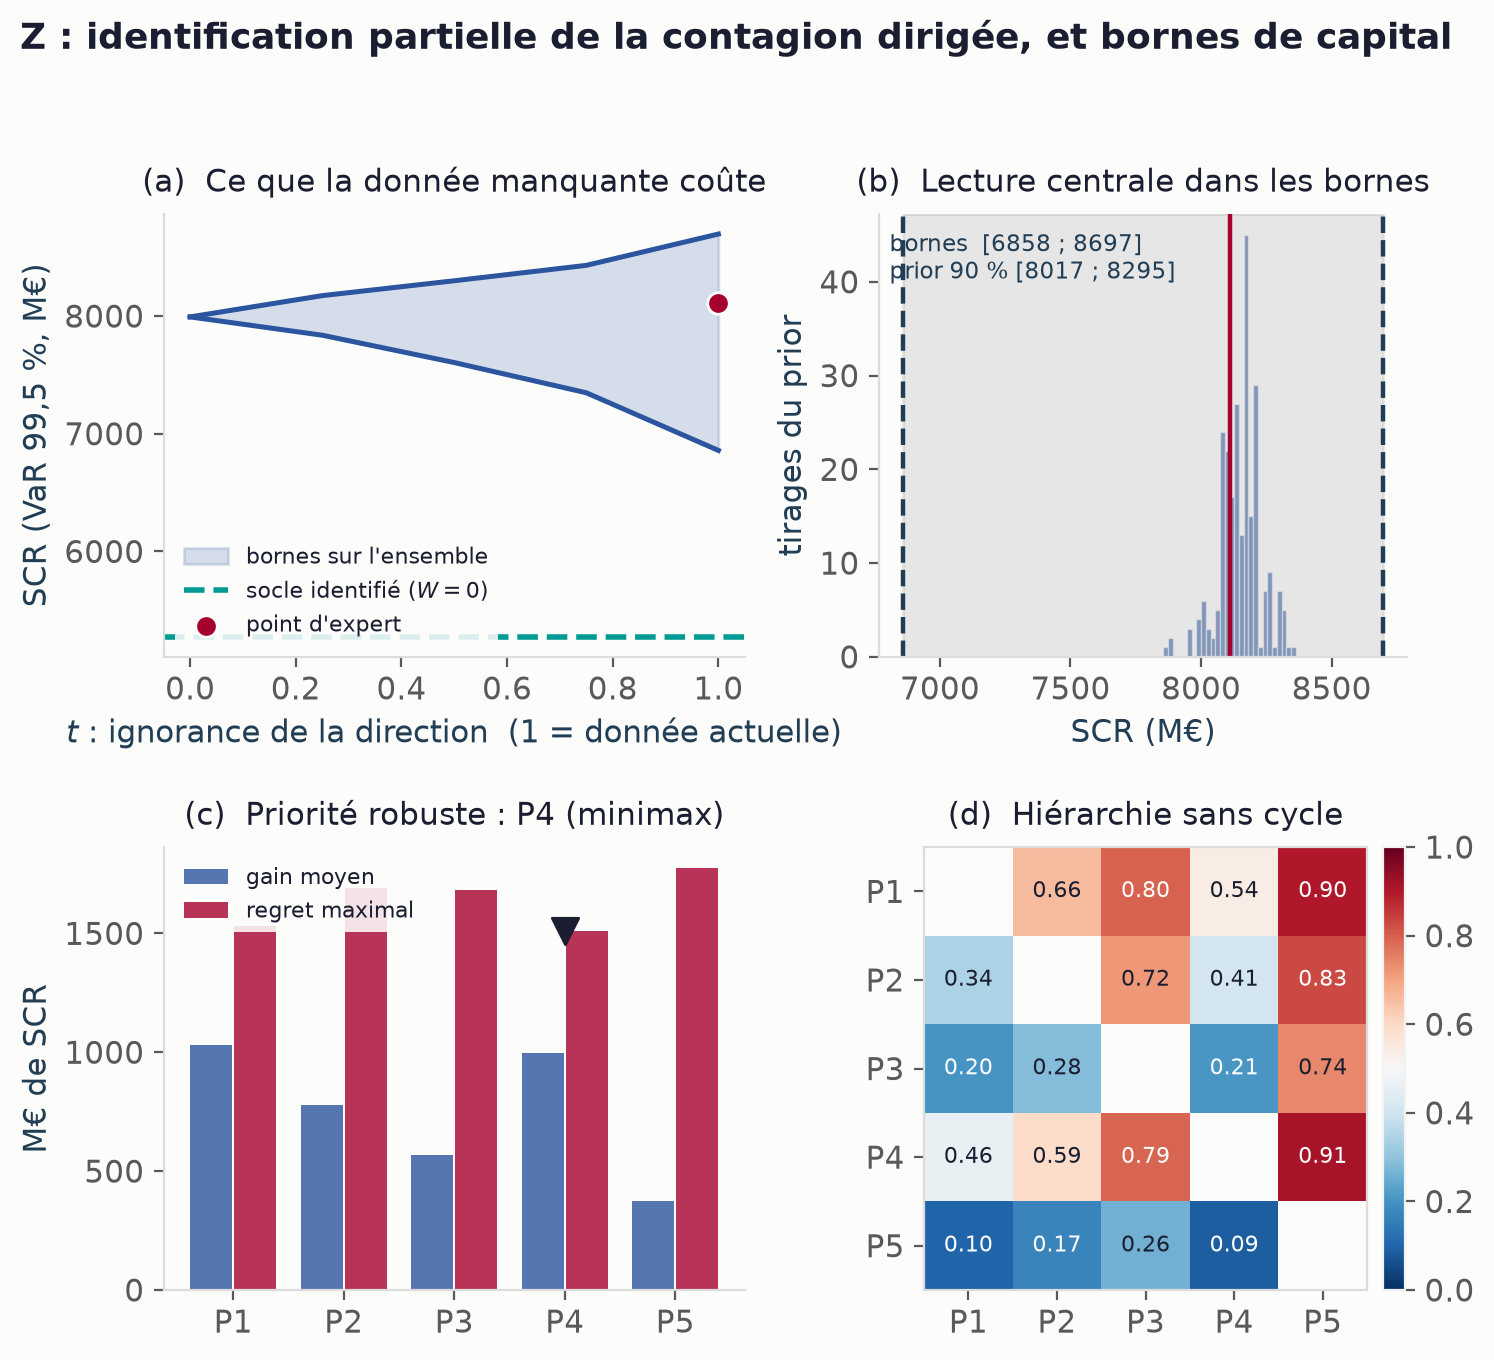
\includegraphics[width=\linewidth]{Z_identification_partielle.png}
\caption{Identification partielle de la contagion dirigée. (a)~Le coût de la donnée
manquante : les bornes se resserrent à mesure que l'ignorance directionnelle $t$ diminue.
(b)~La lecture centrale du prior d'expert, à l'intérieur de bornes qui n'en dépendent pas.
(c)~La priorité de remédiation robuste, au sens du regret maximal. (d)~La dominance
majoritaire entre piliers sur l'ensemble admissible.}
\label{fig:partielle}
\end{figure}

\begin{figure}[htbp]
\centering
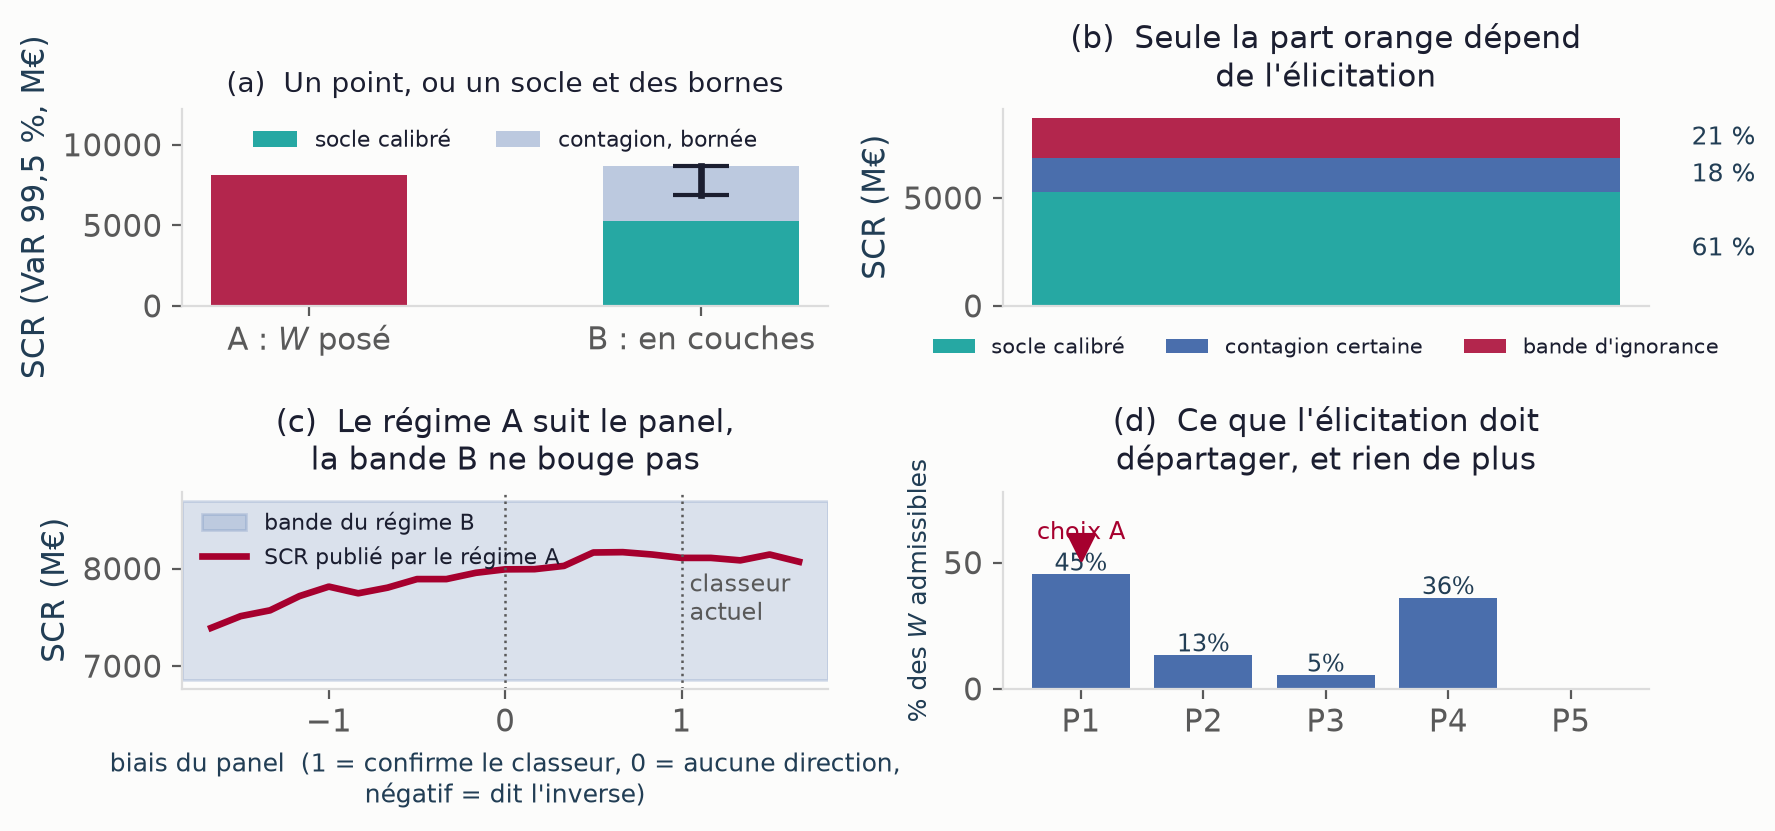
\includegraphics[width=\linewidth]{Z2_comparaison_regimes.png}
\caption{Poser $W$ ou le borner, comparés avant élicitation. (a)~Un point contre un socle
et des bornes. (b)~Seule la part supérieure dépend de l'élicitation. (c)~Le régime~A suit
le biais du panel, la bande du régime~B ne bouge pas. (d)~Ce que l'élicitation doit
départager, et rien de plus.}
\label{fig:regimes}
\end{figure}

\section{L'échelle de repli sur la direction}
\label{sec:echelle-u}

La décomposition $W = S + A$ borne la direction en bloc. On peut faire mieux, en suivant
la méthode d'attaque puis de repli : reparamétrer la propagation par
\[
  \operatorname{logit} p_{ij} \;=\; \operatorname{logit} p_j + u_{ij},
\]
où $p_j$ est l'\textbf{attractivité de la cible} (ce qui subsiste quand la source ne compte
pas) et $u_{ij}$ l'\textbf{excès propre à la source}, c'est-à-dire la direction. La
décomposition n'est identifiée qu'une fois posée la normalisation $\sum_{i\neq j} u_{ij}=0$
pour chaque $j$ : c'est une convention de repérage, et non une information, ce que l'on
vérifie numériquement (une translation compensée de $p_j$ et de $u$ laisse le SCR
strictement inchangé). On descend alors une échelle de crans, du plus ambitieux au repli :
$u$ libre, puis $u$ de \textbf{rang $1$} ($u_{ij}=b_j(a_i-\bar a)$, qui capte $74\,\%$ de
la direction posée et resserre les bornes de $25\,\%$ au prix d'une hypothèse de structure),
puis $u$ élicité, puis $u=0$.

\begin{cle}
\textbf{Le cran nul, et ce qu'il révèle de la contribution.} À $u=0$, la propagation ne
dépend plus que de la cible : \emph{aucune source ne se distingue}. Or c'est exactement là
que P1 et P4, les deux piliers de tête, deviennent \textbf{indiscernables} (gains de
remédiation $1\,051$ contre $1\,052$~M\euro{}, écart nul), alors qu'ils sont séparés de
$353$~M\euro{} dès que la direction du classeur est rétablie. \textbf{La direction est donc
précisément ce qui départage les deux piliers prioritaires} : sans elle, on ne sait plus
lequel remédier d'abord. La contribution du mémoire ne se lit pas sur le niveau d'un
quantile, elle se lit ici, sur une décision qui bascule (figure~\ref{fig:echelle}).
\end{cle}

\begin{figure}[htbp]
\centering
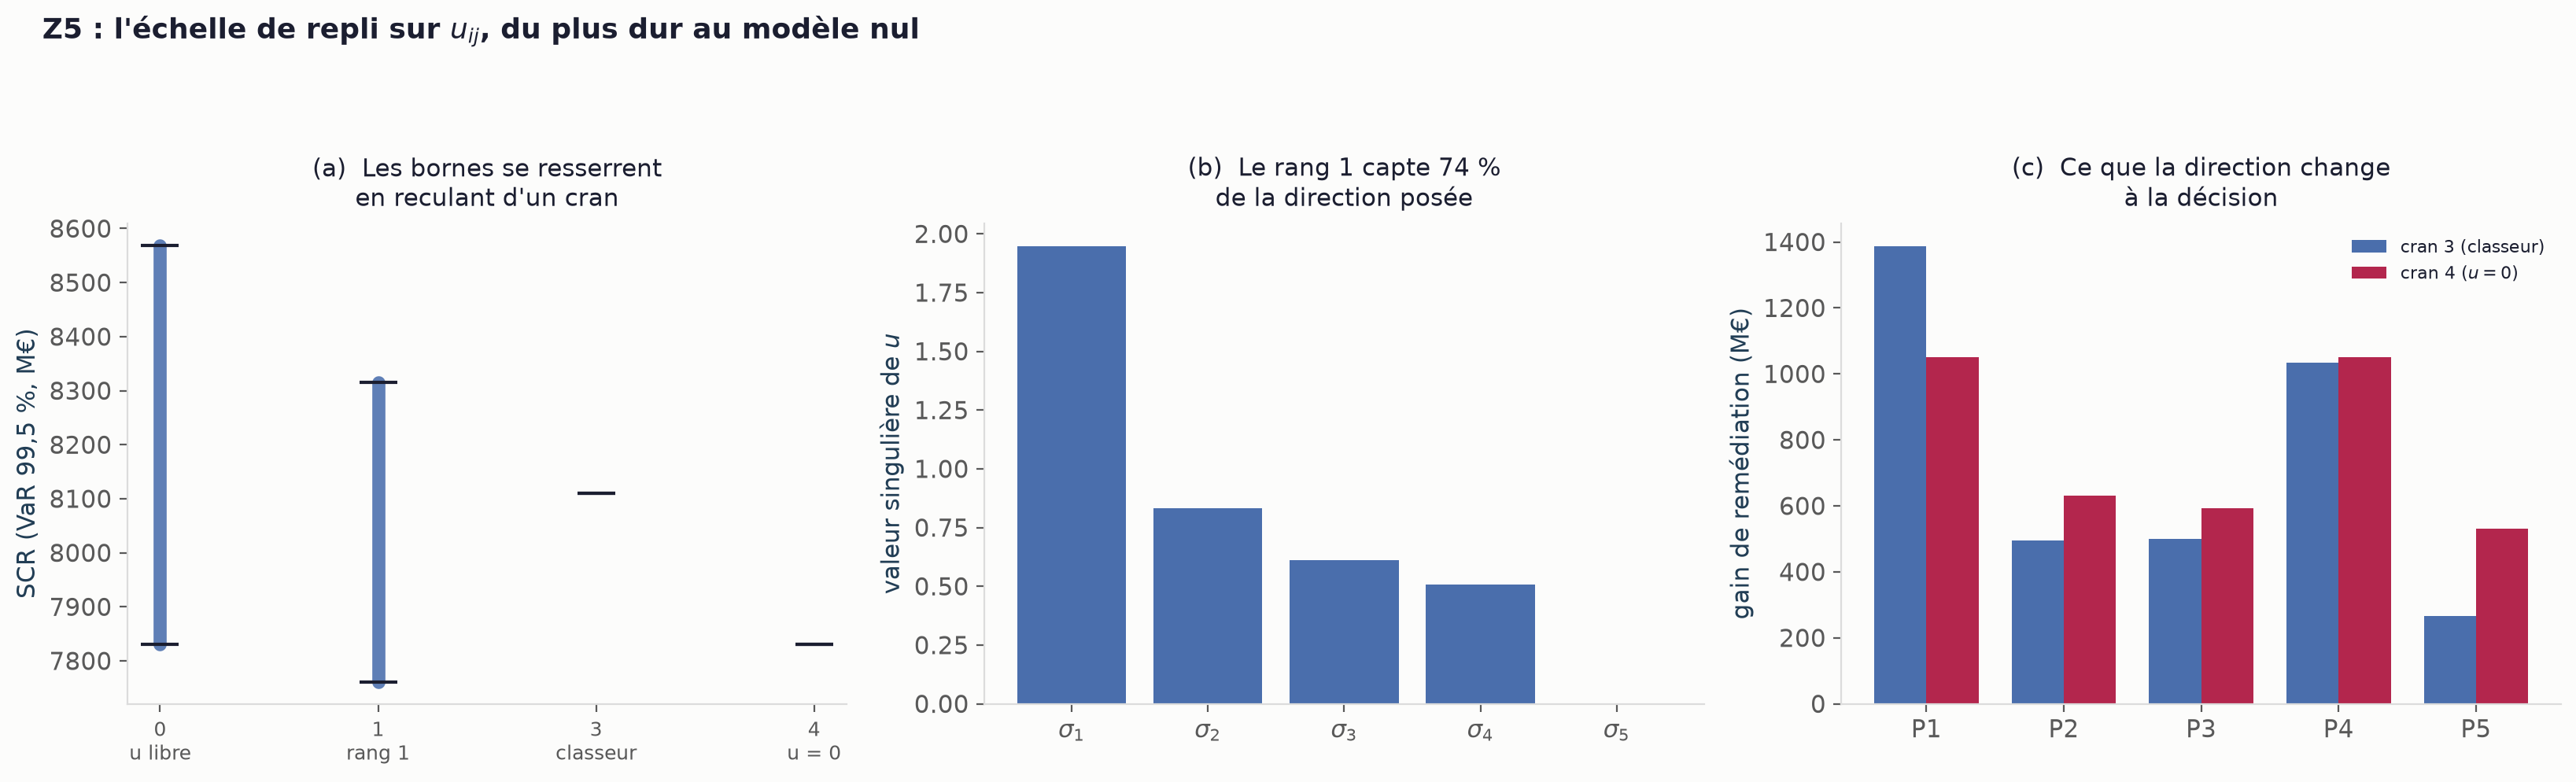
\includegraphics[width=\linewidth]{Z5_echelle_repli.png}
\caption{L'échelle de repli sur $u_{ij}$. (a)~Les bornes de capital se resserrent quand on
recule d'un cran (hypothèse de structure). (b)~Un rang $1$ capte $74\,\%$ de la direction
posée. (c)~Ce que la direction change à la décision : au cran nul, les gains de remédiation
de P1 et P4 se rejoignent.}
\label{fig:echelle}
\end{figure}

% =====================================================================
 % Le capital en bornes sur l'ensemble admissible
\chapter{Résultats}
\label{chap:resultats}

Ce chapitre livre le \og combien \fg{} de la question du mémoire, sous la discipline posée
aux chapitres~\ref{ch:identifiabilite} et~\ref{chap:partielle} : les niveaux sont
illustratifs, les écarts et les ordres sont ce qui résiste. Les capitaux sont calculés à
l'échelle du secteur financier, l'entité type de $15\,000$~M\euro{} de provisions servant de
repère forfaitaire et de cible à la descente d'échelle du \S\ref{sec:ancrage}, avec
deux périmètres de sévérité : OpRisk (grandes pertes opérationnelles, queue lourde)
et PRC (sévérité plafonnée à $40$~M\euro). Sauf mention contraire, on lit la médiane
et l'intervalle interquartile, la variance de la sévérité étant infinie ($\hat\xi=0{,}595$ sur
OpRisk, $1{,}03$ sur PRC).

\begin{attention}
\textbf{Comment lire les niveaux de ce chapitre.} Les montants qui suivent sont
\emph{illustratifs} et ne doivent pas être lus comme la mesure du capital d'une entité réelle.
Le chapitre~\ref{chap:partielle} le démontre : en ne faisant varier que la loi de sévérité et la
fréquence, c'est-à-dire des \emph{entrées} du modèle qui dépendent d'un périmètre de collecte
non transposable, le niveau se déplace d'un facteur $41$, tandis que les rapports au socle
varient d'au plus $33\,\%$ et que le groupe de tête du classement des piliers ne change pas. Le
tableau~\ref{tab:scretat} en donne d'ailleurs l'illustration immédiate : le même état conforme
vaut $8\,301$~M\euro{} sous OpRisk et $2\,589$~M\euro{} sous PRC en lecture~A, soit un
facteur~$3{,}2$ pour un seul changement de périmètre de sévérité, facteur qui n'est pas une
constante et grandit sur le socle sans contagion du chapitre~\ref{chap:partielle}. Ce chapitre établit donc des écarts, des
rapports et des ordres ; ses conclusions reposent sur eux, jamais sur un niveau.
\end{attention}

\begin{cle}
\textbf{Réconciliation avec le socle du chapitre~\ref{chap:partielle}.} Ce chapitre parle d'un
SCR \emph{conforme} d'environ $5\,900$~M\euro{}, quand le chapitre~\ref{chap:partielle} parle
d'un \emph{socle} de $5\,275$~M\euro{}. Ce ne sont pas deux mesures de la même chose, mais deux
points d'un seul modèle : le socle est pris à contagion nulle ($W=0$), là où l'état
conforme en conserve une. L'ordre socle $<$ conforme $<$ non conforme est donc cohérent, et le
pont terme à terme comme l'écart résiduel de Monte-Carlo sont établis
\matcomp.
\end{cle}

% SOURCES-SCRIPTS: 65 66 12 16 63

\section{SCR par état de conformité}

Le SCR croît de façon monotone de l'état conforme à l'état non conforme
(figure~\ref{fig:multietats}). Le tableau~\ref{tab:scretat} donne les trois lectures emboîtées :
la lecture~A porte sur la fréquence seule ; la lecture~B ajoute la
propagation de la cascade ; la lecture~C ajoute le canal détection.

\begin{table}[htbp]\centering\small
\renewcommand{\arraystretch}{1.25}
\begin{tabular}{@{}l ccc c ccc@{}}
\toprule
& \multicolumn{3}{c}{\textbf{OpRisk} (M\euro)} & & \multicolumn{3}{c}{\textbf{PRC} (M\euro)} \\
\cmidrule(lr){2-4}\cmidrule(lr){6-8}
État & A & B & C & & A & B & C \\
\midrule
Conforme               & 8301  & 6664  & 5932  & & 2589 & 1903 & 1642 \\
Partiellement conforme & 11059 & 9625  & 9625  & & 3653 & 3118 & 3118 \\
Non conforme           & 15074 & 15074 & 16595 & & 5520 & 5520 & 6577 \\
\bottomrule
\end{tabular}
\caption{SCR par état, trois lectures (A~: fréquence ; B~: $+$~propagation ; C~:
$+$~détection). Le canal détection ne joue qu'aux extrêmes (il
% SOURCES-SCRIPTS: 16
abaisse l'état conforme et relève le non conforme), l'état partiel n'étant pas modulé.}
\label{tab:scretat}
\end{table}

\subsection*{Le chiffre de tête : quatre lectures emboîtées et la lecture publiée}
\label{sec:chiffre-de-tete}

Le tableau qui précède n'est pas le seul protocole du mémoire à chiffrer \og l'écart entre l'état
conforme et l'état non conforme \fg{}. Quatre le font, et ils donnent quatre résultats. Aucun
n'est faux : ils ne relâchent pas le même nombre de canaux entre les deux états, et rien
d'autre ne les sépare. Les publier sans le dire reviendrait à laisser le lecteur trancher sans les éléments.

\begin{center}\footnotesize
\renewcommand{\arraystretch}{1.25}
\begin{tabular}{@{}l c r r r@{}}
\toprule
\textbf{Lecture} & \textbf{canaux} & \textbf{conforme} & \textbf{non conf.} & \textbf{facteur} \\
\midrule
Score de conformité seul, $g$ figé au niveau NC & 1 & 7987 & 16\,847 & $2{,}11$ \\
Fréquence $+$ propagation (lecture~B) & 2 & 6664 & 15\,074 & $2{,}26$ \\
$+$ détection (lecture~C) & 3 & 5932 & 16\,595 & $2{,}80$ \\
\textbf{$+$ accumulation P4 (les quatre canaux)} & \textbf{4} & \textbf{6049} & \textbf{20\,188}
& $\mathbf{3{,}34}$ \\
\bottomrule
\end{tabular}
\end{center}

\vspace{4pt}
\noindent En M\euro, périmètre OpRisk. Les niveaux sont ceux des sorties versionnées ; les
\emph{rapports}, eux, sont recalculés à chaque exécution plutôt que
calculés à la lecture, faute de quoi un niveau amont pourrait bouger sans que le facteur suive.
% SOURCES-SCRIPTS: 25 16 43 67

\begin{cle}
\textbf{Le mémoire publie la lecture à quatre canaux : $6\,049 \to 20\,188$~M\euro, soit un
facteur $3{,}34$ et un écart de $14\,139$~M\euro.} Le motif n'est pas qu'elle donne le chiffre
le plus grand, c'est qu'elle est la seule où l'état conforme est conforme sur tous les
canaux que le modèle possède. Dans la première lecture, l'entité dite conforme propage encore
comme une entité défaillante ; dans les deux suivantes, sa détection ou son accumulation tiers
restent au niveau non conforme. Une entité conforme sur un canal et non conforme sur trois autres
n'est pas un état conforme, c'est une \emph{remédiation partielle}, et la nommer conforme
sous-estime l'écart par construction.

\textbf{Le canal de détection y est inclus parce que son effet est résolu} : il pèse
$2\,928 \pm 343$~M\euro{} en valeur de Shapley et
$4\,562 \pm 819$ en marginal de fermeture, signe résolu sur seize graines.
% SOURCES-SCRIPTS: 68

\textbf{Les trois autres lectures ne sont pas retirées}, délibérément : ce sont des
remédiations \emph{partielles}, ce qui est un objet utile en soi, et leur emboîtement chiffre ce
que coûte de ne fermer qu'une partie des canaux.
\end{cle}

\begin{attention}
\textbf{Le facteur se compare d'une lecture à l'autre, l'écart en euros non} : l'écart passe de $8\,860$ à $8\,410$~M\euro{}
entre les deux premières lignes alors que le facteur monte. La cause n'est pas un effet de modèle
mais un changement de base, l'état conforme passant de $7\,987$ à $6\,664$~M\euro{} d'un
protocole à l'autre. Un écart en euros ne se compare qu'à base égale ; un rapport est sans
dimension. C'est le même motif qui fait publier des élasticités plutôt que des plages au
\S\ref{sec:sensibilite-propagation}.

\textbf{Et la monotonie du facteur s'observe, elle ne se teste pas ici.} Les quatre lignes ne
forment pas une expérience contrôlée, leurs protocoles différant aussi par la graine et par la
base. Elle est \emph{cohérente} avec la composition des canaux mesurée sur les seize
configurations, qui partagent le même moteur et les mêmes graines : les canaux s'y multiplient
presque exactement, le produit des quatre facteurs isolés valant $3{,}47$ pour un facteur publié
de $3{,}34$, si bien que l'interaction de $5\,001$~M\euro{} en euros est l'arithmétique d'un
produit plus qu'un effet propre de la cascade (\S\ref{sec:inverse}).
% SOURCES-SCRIPTS: 100
% SOURCES-SCRIPTS: 68
\end{attention}

\begin{figure}[htbp]\centering
\figover{S33_treillis_canaux_3d.png}
\caption{Les seize configurations de canaux, rangées par nombre de canaux relâchés. La hauteur
est le capital, les deux extrémités étant les deux états publiés, $6\,049$ et $20\,188$~M\euro{} ;
tout sommet intermédiaire est une remédiation partielle. Chaque arête monte, ce qui est la
monotonie du \S\ref{sec:inverse} lue d'un coup d'\oe{}il. La couleur est l'écart à l'additivité,
c'est-à-dire le capital observé moins la somme des quatre effets isolés : elle vaut $+5\,001$ au
sommet complet et $-330$ sur la seule paire négative du dossier, propagation et accumulation. Le
troisième axe sépare les configurations de même rang et ne porte aucune grandeur.}
% SOURCES-SCRIPTS: 68 108
\label{fig:treillis-canaux}
\end{figure}

\noindent\textbf{Où chaque lecture continue de servir.} Les trajectoires du
\S\ref{sec:res-traj} et la priorisation du \S\ref{sec:res-prio} restent conduites en
\emph{lecture~B}. Ce n'est pas une indécision résiduelle mais un choix d'objet : elles portent
sur l'\emph{ordre} de remédiation, dont le chapitre~\ref{ch:robustesse} montre qu'il est
invariant aux leviers testés, de sorte que le canal ajouté déplacerait leurs niveaux sans
déplacer leur conclusion. Les rejouer relèverait par ailleurs de la recalibration, que le gel
interdit.

\begin{figure}[htbp]\centering
\figover{S10_scr_multi_etats.png}
\caption{SCR par état de conformité (trois canaux emboîtés) et bascule des états en crise
systémique.}
% SOURCES-SCRIPTS: 16
\label{fig:multietats}
\end{figure}

Le surcoût de non-conformité $\Delta_{\text{DORA}}=\mathrm{SCR}(\text{NC})-\mathrm{SCR}(\text{C})$,
à graine Monte-Carlo commune (l'écart ne vient que du changement d'état, non du bruit),
s'obtient par bootstrap deux niveaux (multiplicateurs $+$ sévérité), et $100\,\%$ des tirages
sont positifs.

\begin{table}[htbp]\centering\small
\renewcommand{\arraystretch}{1.25}
\begin{tabular}{@{}l cc@{}}
\toprule
& médiane & IC90\,\% \\
\midrule
$\Delta_{\text{DORA}}$ NC vs C (OpRisk) & 7401 & $[2830\,;38793]$ \\
$\Delta_{\text{DORA}}$ PC vs C (OpRisk) & 2556 & $[963\,;12768]$  \\
$\Delta_{\text{DORA}}$ NC vs C (PRC)    & 3668 & $[3201\,;4094]$  \\
$\Delta_{\text{DORA}}$ PC vs C (PRC)    & 1257 & $[1077\,;1466]$  \\
\bottomrule
\end{tabular}
\caption{Surcoût de non-conformité en euros (M\euro), lecture B (fréquence $+$ propagation),
bootstrap deux niveaux. Côté OpRisk la sévérité de queue est ré-échantillonnée sur les
$91$ excès réels, non tirée dans une approximation
% SOURCES-SCRIPTS: 14
normale~; l'intervalle reste large parce que la queue l'est, non par artefact de méthode.}
% SOURCES-SCRIPTS: 16
\label{tab:delta}
\end{table}

\noindent \textbf{Lecture actuarielle.} L'intervalle très large côté OpRisk
(table~\ref{tab:delta}) n'est pas un défaut
du modèle : c'est la signature d'une queue d'indice $0{,}60$, où le niveau du capital est
intrinsèquement imprécis. L'écart typique (interquartile) est bien plus resserré que
l'intervalle à $90\,\%$, et le \emph{signe} du surcoût, lui, est certain. On retrouve la thèse du
mémoire : le SCR est une distribution, pas un point.

\paragraph{L'intervalle PRC est étroit, et il le reste quand on cesse de croire la conversion
exacte.} La sévérité PRC est dérivée du nombre d'enregistrements compromis par la relation
log-log de \citet{jacobs2014}, dont le résidu vaut $0{,}523$ en logarithme naturel : à volume donné,
le coût réel varie d'un facteur $2{,}4$ autour de la droite à $90\,\%$. Réinjecter ce résidu
% SOURCES-SCRIPTS: 21
enregistrement par enregistrement ne rouvre pourtant presque pas l'intervalle, le bruit se
moyennant dans l'ajustement GPD ; il déplace le \emph{niveau} du surcoût de $7\,\%$, sans
l'élargir \matcomp. L'étroitesse de l'intervalle PRC n'est donc pas un artefact
de la conversion déterministe.

\section{Décomposition par pilier}

En basculant un pilier à la fois de conforme à non conforme, le surcoût se décompose
(figure~\ref{fig:decomp}). Le classement obtenu, $P1>P4>P2>P3>P5$, reproduit exactement
le classement ROOT du modèle qualitatif. La convergence n'est pas une validation
indépendante : les amorces de la cascade sont semées selon ROOT (\S\ref{sec:allocation}), et ROOT
se déduit de la même matrice d'expert que $W$ (\S\ref{sec:branch}). Elle atteste la cohérence
du modèle avec son jugement d'origine.

\begin{figure}[htbp]\centering
\figover{S11_decomp_par_pilier.png}
\caption{Décomposition du $\Delta_{\text{DORA}}$ par pilier et validation croisée avec ROOT.
}
% SOURCES-SCRIPTS: 16b
\label{fig:decomp}
\end{figure}

\begin{cle}
\textbf{Une interaction super-additive, établie là où l'estimateur est fiable.} Les surcoûts
isolés ne somment pas au surcoût total : il reste un terme d'\emph{interaction}, signature de la
cascade (un pilier non conforme amplifie aussi les contagions amorcées ailleurs qui le
traversent), qu'un modèle sans propagation (un LDA à copule) ne peut pas produire.
Sa mesure exige toutefois de la prudence : une interaction est une différence de différences,
l'estimateur Monte-Carlo le plus fragile qui soit en queue lourde. Sur la VaR à $99{,}5\,\%$
OpRisk, son \emph{signe n'est pas résolu} : sur six graines à résolution égale
($60\,000$ années chacune), il va de $-137$ à $+1\,395$~M\euro{} et n'est positif que dans
quatre cas sur six, la graine de référence donnant $+1\,395$~M\euro{}. Un estimateur
qui change de signe avec la graine interdit d'en tirer quoi que ce soit. La super-additivité
est en revanche robuste partout où le bruit de queue ne domine pas : en \emph{perte moyenne}
elle est positive sur les six graines ($+532$ à $+659$~M\euro{} OpRisk, $+827$
côté PRC, soit environ un cinquième du surcoût moyen), et jusque dans la VaR du périmètre PRC,
dont le plafond de sévérité tronque la queue ($+905$~M\euro{}). Conséquence pratique : puisque les
marginaux ne somment pas au total, l'attribution du surcoût aux piliers exige une règle
principielle qui somme exactement : c'est l'objet de la valeur de Shapley
(section~\ref{sec:allocation}). À ne pas confondre avec l'interaction entre les quatre
\emph{canaux} de la non-conformité, qui décompose le même écart sur une autre partition, vaut
$+5\,001$~M\euro{} et dont le signe, lui, \emph{est} résolu : elle est reprise terme par terme au
\S\ref{sec:kpi}. Les deux ne s'additionnent pas.
% SOURCES-SCRIPTS: 16b 20b 68
\end{cle}

\section{Allocation du capital : Shapley et Euler}
\label{sec:allocation}

La décomposition qui précède pose deux questions d'allocation distinctes. \emph{Qui porte le
surcoût~?} appelle une attribution par pilier \emph{source} de la non-conformité, qui doit
composer avec l'interaction (les marginaux ne somment pas au total). \emph{Où loge le
capital~?} appelle une allocation du niveau $\mathrm{SCR}(\text{NC})$ par pilier
\emph{touché}, cohérente au sens où les parts somment au total. La valeur de Shapley répond
à la première, la règle d'Euler à la seconde (%
% SOURCES-SCRIPTS: 20
figure~\ref{fig:allocation}).

\subsection{Shapley : attribuer le surcoût, interaction comprise}

On munit les piliers d'une fonction caractéristique
\[
v(S) \;=\; \mathrm{SCR}\bigl(S \text{ en NC},\ \text{reste C}\bigr)-\mathrm{SCR}(\text{tous C}),
\qquad S \subseteq \{P1,\dots,P5\},
\]
calculée par la cascade sur les $2^5$ configurations à graine Monte-Carlo commune. Le
marginal de la section précédente est $v(\{k\})$~; la valeur de Shapley
\[
\varphi_j \;=\; \sum_{S \subseteq \{P1,\dots,P5\}\setminus\{j\}}
\frac{|S|!\,\bigl(5-|S|-1\bigr)!}{5!}\,\bigl[v(S\cup\{j\})-v(S)\bigr]
\]
moyenne la contribution de $j$ sur tous les ordres d'arrivée. Par efficience,
$\sum_j \varphi_j = v(\text{tous}) = \Delta_{\text{DORA}}$ \emph{exactement} : la règle
redistribue l'interaction que les marginaux isolés laissent de côté, quel que soit son signe.

La construction est celle de \citet{Shapley1953}, dont l'efficience est la propriété
axiomatique ; son emploi en allocation de capital remonte à \citet{denault2001}, et son usage
actuariel sous Solvabilité~II est documenté \citep{Decupere2011}. Les cinq piliers autorisent l'énumération exacte des $5!$
ordres d'arrivée ; les algorithmes par échantillonnage des permutations
\citep{CastroGomezTejada2009, SongNelsonStaum2016}, indispensables en grande dimension, ne
sont donc pas nécessaires ici, et aucune approximation n'entre dans le tableau qui suit.

\begin{table}[htbp]\centering\small
\renewcommand{\arraystretch}{1.25}
\begin{tabular}{@{}l rrr c rrr@{}}
\toprule
& \multicolumn{3}{c}{OpRisk} & & \multicolumn{3}{c}{PRC} \\
\cmidrule{2-4}\cmidrule{6-8}
pilier & marginal & $\varphi_j$ & part & & marginal & $\varphi_j$ & part \\
\midrule
P1 gouvernance & 3481 & 3717 & $34{,}0\,\%$ & & 1375 & 1608 & $32{,}4\,\%$ \\
P4 tiers       & 2658 & 2810 & $25{,}7\,\%$ & & 1075 & 1252 & $25{,}3\,\%$ \\
P2 incidents   & 1634 & 1867 & $17{,}1\,\%$ & &  721 &  920 & $18{,}6\,\%$ \\
P3 tests       & 1094 & 1484 & $13{,}6\,\%$ & &  571 &  738 & $14{,}9\,\%$ \\
P5 partage     &  665 & 1048 &  $9{,}6\,\%$ & &  311 &  438 &  $8{,}8\,\%$ \\
\midrule
somme          & 9531 & 10\,927 & $100{,}0\,\%$ & & 4052 & 4957 & $100{,}0\,\%$ \\
\bottomrule
\end{tabular}
\caption{Valeur de Shapley du surcoût $\Delta_{\text{DORA}}$ (M\euro, NC vs C, trois canaux,
protocole des trois canaux). Les marginaux somment à $9\,531$ (OpRisk), la valeur de
% SOURCES-SCRIPTS: 16b
Shapley à $10\,927$, le surcoût total exactement. Cellules arrondies au million et parts au
dixième de point, échelle à laquelle la colonne somme exactement à cent : c'est la propriété
d'efficacité de la valeur de Shapley, et elle se lit dans le tableau plutôt que de s'y
excuser en note.}
% SOURCES-SCRIPTS: 20
\label{tab:shapley}
\end{table}

Le classement de Shapley reproduit le classement ROOT sur les deux périmètres. Une part de
cette convergence est mécanique : les amorces de la cascade sont semées
proportionnellement à ROOT (parts $30/27/18/15/9\,\%$),
% SOURCES-SCRIPTS: 20
et le canal fréquence d'un pilier
module sa propre part d'amorce. Le test non trivial est la \emph{déformation} : la part de
Shapley de P1 ($34\,\%$) excède sa part d'amorce ($30\,\%$), effet propre de la propagation
(P1 est l'émetteur le plus fort de $W$), et l'interaction redistribuée ($+1\,395$~M\euro{}
OpRisk, $+905$ PRC à cette graine) est intégralement un produit de la cascade, absent d'un
modèle additif.

\subsection{Euler : allouer le niveau, et une limite d'estimation assumée}

La règle d'Euler \citep{tasche1999} alloue $\mathrm{SCR}(\text{NC})$ par
$C_j = \mathbb{E}\bigl[L_j \mid L \ge \VaR_{99{,}5\,\%}\bigr]$ (version TVaR, exacte
par construction), où $L_j$ est la perte du pilier \emph{touché} $j$ dans la cascade. Côté
PRC, l'allocation est stable et presque plate : P2 $23\,\%$, P4 $23\,\%$, P1 $20\,\%$,
P3 $18\,\%$, P5 $17\,\%$, et les parts de capital coïncident avec les parts de perte moyenne
parce que le plafond de sévérité tronque la queue
($\TVaR = 6\,795 \approx \VaR = 6\,573$~M\euro). Côté OpRisk, les parts
\emph{moyennes} sont stables (P2 $23\,\%$, P4 $22\,\%$, P1 $20\,\%$, P3 $18\,\%$,
P5 $16\,\%$), mais l'allocation de la queue extrême ne l'est pas, et la cause en est
théorique : avec $\xi \approx 0{,}6 > 0{,}5$, la sévérité est de variance infinie,
l'estimateur Monte-Carlo de la TVaR converge en régime de loi stable, et le classement
conditionnel bascule d'une résolution à l'autre (vérifié à $150$ et $240$~mille années
simulées). On rapporte donc l'allocation de queue du périmètre PRC, régularisée par le cap,
et l'on tient celle d'OpRisk pour indicative.

\paragraph{La mesure de queue sert ici à \emph{mesurer}, jamais à couvrir.} La distinction est
assez souvent négligée pour qu'il faille l'écrire. Le besoin de capital publié dans ce mémoire
est partout un $\VaR_{99{,}5\,\%}(L)$ centré, conformément au niveau de Solvabilité~II ; aucune
grandeur de couverture n'est une TVaR, ni une CTE, ni un Expected Shortfall. La mesure
de queue intervient à deux titres, et tous deux sont des titres de \emph{diagnostic}. Comme
noyau d'allocation d'abord, dans la règle d'Euler ci-dessus, où elle répartit un niveau déjà
fixé sans le modifier. Comme \emph{indicateur de forme de queue} ensuite : le rapport
$\TVaR_{99{,}5\,\%}(L)/\VaR_{99{,}5\,\%}(L) \approx 2{,}1$ se compare à son asymptote théorique
$1/(1-\xi) = 2{,}5$. L'information est portée par ce rapport, non par les deux montants.
% SOURCES-SCRIPTS: 67
Ce rapport dépend de l'état et il faut
donc dire lequel : $2{,}10$ vaut à l'état \emph{tous non conforme}, celui de cette section, tandis
qu'il vaut $2{,}17$ sur la calibration de référence \matcomp. Les deux
% SOURCES-SCRIPTS: 73
valeurs sont justes, elles ne portent pas sur la même loi de perte, et l'écart entre elles est
sans signification en soi.

Deux raisons de ne pas en faire un niveau de couverture, dont la seconde est décisive. La
première est de proportion : sur un risque aussi large, dont les queues sont plurielles selon la
catégorie d'événement (chapitre~\ref{chap:adaptations}), adosser la couverture à une moyenne de queue
déformerait la distribution et immobiliserait un capital sans commune mesure avec le niveau
réglementaire de référence. La seconde est d'existence : sous la calibration PRC,
$\hat\xi=1{,}033>1$ place la sévérité en régime d'espérance infinie, et la mesure
n'existe alors pas au sens mathématique. Une mesure de couverture qui cesse d'être définie
selon la source de sévérité retenue ne peut pas porter un besoin de capital ; le même objet,
lu comme un diagnostic de queue, reste au contraire parfaitement informatif, puisque sa
divergence \emph{est} l'information.

\begin{cle}
\textbf{Sources et réceptacles.} Les deux allocations ne racontent pas la même chose, et
c'est le résultat : Shapley, vue \emph{source}, concentre le surcoût sur P1 ($34\,\%$), là
où naît la non-conformité~; Euler, vue \emph{réceptacle}, répartit le capital presque
uniformément sur les piliers touchés (P2 et P4 en tête légère). La remédiation se décide
côté source~; le capital, lui, se loge là où les cascades atterrissent.
\end{cle}

\begin{figure}[htbp]\centering
\figover{S15_allocation_shapley_euler.png}
\caption{Allocation du capital DORA (OpRisk). (a)~Shapley contre marginaux : l'interaction
redistribuée. (b)~Euler : parts de capital (queue) contre parts de perte moyenne~; sur ce
périmètre non plafonné, l'allocation fine de la queue extrême reste indicative
($\xi \approx 0{,}6$, variance de sévérité infinie).}
% SOURCES-SCRIPTS: 20
\label{fig:allocation}
\end{figure}

\section{Trajectoire du capital}
\label{sec:res-traj}

Le long de la mise en conformité, le capital décroît de l'état initial vers le SCR conforme, et
le surcoût résiduel $\Delta_{\text{DORA}}(t)$ tend vers zéro (tableau~\ref{tab:traj},
figure~\ref{fig:traj}). Partant de l'état marginal actuel (NC~$35\,\%$, PC~$35\,\%$, C~$30\,\%$),
le capital OpRisk passe de $\sim 10\,750$ à $\sim 7\,040$~M\euro{} sur cinq ans, vers le SCR
conforme ($\sim 6\,925$).

\begin{table}[htbp]\centering\small
\renewcommand{\arraystretch}{1.2}
\begin{tabular}{@{}c ccc@{}}
\toprule
$t$ (ans) & SCR($t$) médiane & bande 90\,\% & $\Delta_{\text{DORA}}(t)$ \\
\midrule
0 & 10752 & $[9092\,;12654]$ & 3827 \\
1 & 9576  & $[7205\,;12040]$ & 2652 \\
2 & 8310  & $[6194\,;11042]$ & 1385 \\
3 & 7575  & $[5924\,;10164]$ & 650 \\
5 & 7041  & $[5857\,;9028]$  & 116 \\
\bottomrule
\end{tabular}
\caption{Trajectoire du capital DORA (M\euro, OpRisk).}
% SOURCES-SCRIPTS: 17
\label{tab:traj}
\end{table}

\begin{figure}[htbp]\centering
\figover{S12_trajectoire_scr.png}
\caption{Trajectoire SCR($t$) et évolution des états de conformité.}
% SOURCES-SCRIPTS: 17
\label{fig:traj}
\end{figure}

\noindent \textbf{Lecture actuarielle.} L'intégrale de la trajectoire, à un coût de capital
près, est le \emph{coût de portage} de la non-conformité pendant la remédiation. La bande reste
large et surtout haute en environnement dégradé : la vraie exposition n'est pas le capital
médian, c'est le risque que la remédiation traîne quand la menace monte, précisément le scénario
où le capital importe le plus.

\section{Priorisation de la remédiation}
\label{sec:res-prio}

Sous budget contraint (un pilier remédié à la fois), l'énumération des $120$ ordres donne
l'ordre optimal $P1\to P4\to P2\to P3\to P5$, égal à l'ordre ROOT et distinct de l'ordre
glouton par valeur d'accélération (figure~\ref{fig:prio}). L'écart de capital intégré entre le
pire ordre et l'optimal atteint $21\,\%$.

\begin{figure}[htbp]\centering
\figover{S13_priorisation.png}
\caption{Valeur d'accélération par pilier et ordre de remédiation optimal.}
% SOURCES-SCRIPTS: 18
\label{fig:prio}
\end{figure}

\begin{cle}
\textbf{Le myope n'est pas l'optimal.} Remédier au coup par coup le pilier au plus fort gain
immédiat (l'ordre glouton) coûte plus cher que l'ordre optimal, parce que les interactions de
cascade imposent de raisonner sur l'horizon entier. L'optimum coïncide avec le classement
ROOT, comme la progéniture (\S\ref{sec:branch}) et la décomposition par pilier ; ces trois
convergences attestent la cohérence du modèle avec le jugement dont il procède, non une
validation indépendante, ROOT entrant dans les amorces.
\end{cle}

\paragraph{La question réciproque donne le classement qu'un plan de
remédiation utilise.} Tout ce qui précède fixe un état et lit un capital. L'exercice de
résistance \emph{inverse} fixe le capital et cherche les états qui le produisent. Un dispositif ORSA emploie un modèle sous
cette forme. La monotonie établie au \S\ref{sec:kpi} le
rend court : l'ensemble des configurations atteignant une cible est croissant, donc entièrement
décrit par ses éléments minimaux, et il n'en compte jamais plus de quatre sur seize. Deux nombres
résument alors tout le treillis. Le canal de fréquence seul atteint $10\,377$~M\euro,
soit $1{,}72$ fois l'état conforme, tandis que les trois autres canaux \emph{réunis} n'atteignent
que $11\,413$, soit $1{,}89$ fois. Toute cible sous le premier seuil se produit donc par un canal
unique, et toute cible au-dessus du second exige la fréquence. Aucun autre canal, seul et
dans sa plage déclarée, n'atteint même $8\,000$~M\euro. La lecture directe hiérarchise les canaux
par leur contribution ; la lecture inverse désigne celui dont la maîtrise \emph{interdit} les
scénarios sévères. L'information n'est pas la même. Détail, frontières par cible et réserves
au \S\ref{sec:inverse}.
% SOURCES-SCRIPTS: 92

\section{Robustesse}

Le niveau du capital bouge fortement selon les leviers non calibrés (l'indice de queue $\xi$
domine, facteur $\sim 6$), mais la direction ($\Delta_{\text{DORA}}>0$) et la
\emph{priorité} (P1 en tête) tiennent sur tous les réglages testés (figure~\ref{fig:robust}).

\begin{figure}[htbp]\centering
\figover{S14_robustesse_multietats.png}
\caption{Robustesse : le classement tient, le niveau non.}
% SOURCES-SCRIPTS: 19
\label{fig:robust}
\end{figure}

\begin{cle}
\textbf{La recommandation ne dépend d'aucun paramètre non mesurable.} L'ordre de remédiation
optimal ne dépend que des SCR par configuration, donc il est invariant aux taux de
transition de la chaîne de Markov, pourtant les paramètres les moins calibrables. Ces taux
fixent le calendrier de la trajectoire, jamais la séquence recommandée. Le verdict d'ensemble
rejoint celui de toute la démarche : le classement est robuste là où le niveau ne l'est pas.
\end{cle}

\begin{attention}
\textbf{Le périmètre exact de cette robustesse.} Les tests ci-dessus font
varier les paramètres du modèle \emph{à matrice $W$ fixée}, celle du classeur qualitatif. Ils
établissent donc que P1 arrive en tête \emph{si l'on admet cette direction}. Dès lors que l'on
admet ne pas connaître la direction et que l'on balaie l'ensemble admissible
(chapitre~\ref{chap:partielle}), P1 et P4 deviennent pratiquement à égalité : P1 arrive
premier dans $43{,}6\,\%$ des configurations, P4 dans $37{,}7\,\%$, et l'écart de regret maximal entre
% SOURCES-SCRIPTS: 30
les deux n'est que de $1{,}5\,\%$. Les deux énoncés ne se contredisent pas, ils portent sur des
sources d'incertitude différentes. Ce qui est robuste dans les deux cadres, c'est que P1 et P4
devancent nettement P2, P3 et P5, et que P5 n'arrive \emph{jamais} en tête.

\medskip
\noindent\textbf{Une troisième source d'incertitude, et elle vise directement le corpus.} Les
rapports post-incident sont des enquêtes officielles, mandatées pour établir une cause racine ;
elles sur-attribuent donc structurellement à la gouvernance, ce que le
chapitre~\ref{ch:identifiabilite} déclare sans pouvoir le lever. On peut néanmoins en chiffrer la
conséquence, en dégradant l'émission de P1 par $W_{1k}\to(1-a)W_{1k}$ et en recalculant l'ensemble
admissible à chaque degré. Le classement tient jusqu'à $a=0{,}25$ et bascule vers P4 à
$a=0{,}50$ : il faut donc supposer la moitié des arêtes issues de la gouvernance
artefactuelles pour renverser la priorité. Le niveau, lui, ne perd que $24{,}8\,\%$ même à
$a=1$, soit $0{,}81$ fois la largeur de la bande d'identification. Le niveau résiste, le
classement non, le seuil est connu.
% SOURCES-SCRIPTS: 64
\end{attention}

\paragraph{Les hypothèses restantes ont leur axe de stress.} Trois entrées ne figuraient pas au
tornado : les coefficients de la conversion Jacobs, la charge systémique $\gamma$ et l'ancrage
des probabilités d'état. Stressées à $\pm 1{,}645$ écart-type, elles déplacent des niveaux sans
jamais toucher la direction ni le classement : le surcoût PRC reste contenu entre $3\,125$ et
$3\,977$~M\euro{} autour du central, $\gamma$ ne commande que la sévérité de la bascule en
crise, et l'ancrage des probabilités d'état déplace le capital espéré actuel mais laisse
inchangés le SCR par état et le surcoût NC contre C, qui lui sont conditionnels. Le détail du
protocole de stress est déporté \matcomp.
% SOURCES-SCRIPTS: 22 67

\section{La sensibilité aux probabilités de propagation, prise pour elle-même}
\label{sec:sensibilite-propagation}

% SOURCES-SCRIPTS: 15 76 30 66 68

Le modèle repose sur des probabilités de propagation qui ne sont pas observées. Cette section
leur consacre un examen séparé, en
distinguant deux questions que l'on confond volontiers : la sensibilité au \emph{niveau} de la
propagation, qui est un facteur d'échelle posé, et la sensibilité à sa \emph{direction}, qui
n'est pas identifiable. La première se stresse, la seconde se borne.

\paragraph{Le niveau de propagation est le levier le moins sensible.} Mesurée en élasticités, à
perturbation relative de $10\,\%$ appliquée à un paramètre à la fois, la sensibilité classe les
leviers comme suit.

\begin{center}\footnotesize
\renewcommand{\arraystretch}{1.15}
\begin{tabular}{@{}l l r@{}}
\toprule
\textbf{Levier} & \textbf{Statut} & \textbf{Élasticité} \\
\midrule
Indice de queue $\xi$ & estimé & $3{,}79$ \\
Échelle $\sigma$ & estimé & $0{,}97$ \\
Taux de dépassement $p_u$ & estimé & $0{,}82$ \\
Fréquence $\lambda$ & estimé & $0{,}45$ \\
Sur-dispersion $\varphi$ & posé & $-0{,}44$ \\
\textbf{Gain de propagation} $\boldsymbol{g}$ & \textbf{posé} & $\mathbf{0{,}37}$ \\
Seuil $u$ seul & choix de méthode & $0{,}03$ \\
\bottomrule
\end{tabular}
\end{center}

\vspace{4pt}
\noindent La propagation a l'élasticité la plus faible des leviers substantiels, $0{,}37$ contre
$3{,}79$ pour l'indice de queue. L'ablation le confirme par un autre chemin : retirer la
propagation fait tomber la VaR de $20\,\%$, retirer la queue lourde de $76\,\%$. La thèse ne
dépend pas des trois valeurs posées de $g$, le capital étant croissant en $g$
(\S\ref{sec:invariance-g}). La direction, elle, ne se stresse pas, elle se borne : à ignorance
totale la largeur de l'ensemble admissible vaut $1\,839$~M\euro, soit $34{,}9\,\%$ du socle, et
elle se paye linéairement avec le degré d'ignorance. Le motif qui écarte les indices de Sobol, la
variance de la charge annuelle n'existant pas, le tornado brut et ses deux défauts, la gradation
de l'ignorance, l'ablation et la comparaison avec le préprint de cascade climatique, qui classe
les leviers à l'inverse parce que sa sévérité est bornée, sont déportés
\matcomp.
% SOURCES-SCRIPTS: 81

\begin{cle}
\textbf{Ce que cette section établit.} La sensibilité aux probabilités de propagation est
\emph{bornée par construction} et non estimée : c'est la différence entre un modèle qui pose une
direction et un modèle qui assume ne pas la connaître. Et elle n'est pas le point faible du
dispositif : le niveau de propagation déplace le capital moins que tout autre levier, tandis que
le seuil de la loi de queue le fait passer à lui seul de $4\,862$ à $12\,944$~M\euro. Toute vigilance sur les
valeurs numériques du modèle doit donc se porter d'abord sur l'ajustement de valeurs extrêmes,
et c'est là que le mémoire concentre ses réserves déclarées.
\end{cle}

\section{Comparaison de modèles : la dépendance n'est pas le mécanisme}
\label{sec:benchmark}

La cascade dirigée remplace ici l'agrégation par copule d'un modèle LDA. Ce que ce
remplacement apporte se mesure en confrontant la cascade à des jumeaux copule construits pour lui
ressembler (figure~\ref{fig:benchmark}, périmètre OpRisk, graines
% SOURCES-SCRIPTS: 23
Monte-Carlo communes). Cette section compare les modèles sur l'axe de la \emph{structure de
dépendance}, à marges fixées ; la comparaison sur l'axe de la \emph{famille de loi} (la bande
de modèle) est conduite en partie~\ref{part:limites}, section~\ref{sec:trois-etages}, et les
deux se complètent.

\textbf{La photo.} À marges par pilier \emph{identiques} (celles de la cascade, état
conforme) et corrélation calée, la copule gaussienne retombe sur le SCR de la cascade
($+0{,}1\,\%$) : en queue lourde ($\xi \approx 0{,}6$), la queue annuelle obéit au principe
de la perte unique dominante et le \emph{niveau} de base n'identifie pas la dépendance. La
Student ($\nu = 4$) le surestime de $17\,\%$ en forçant des co-extrêmes que le mécanisme ne
produit pas ($2{,}28$ piliers extrêmes par année de queue contre $1{,}12$). Le choix de
copule est donc à la fois non identifiable et conséquent~; la cascade n'a pas ce degré de
liberté : sa dépendance est produite par le mécanisme, pas choisie.

\textbf{Et ce résultat a été répliqué ailleurs, sans lien avec ce travail.} L'objection naturelle
serait qu'une coïncidence à $+0{,}1\,\%$ entre une copule gaussienne et un mécanisme de cascade
tient à un réglage particulier du protocole. Le préprint de cascade climatique cité au
chapitre~\ref{ch:positionnement} \citep{ccrn2026} conduit la même expérience, à marges appariées,
entre une gaussienne, une Student et sa propre cascade : il obtient des primes centrales
pratiquement indiscernables et ne voit la séparation apparaître qu'en \emph{queue}. Même
protocole, même conclusion, sur un autre péril et par une autre équipe. Ce n'est donc pas un
artefact du réglage retenu ici, mais une propriété du principe de la perte unique dominante,
qui rend le niveau central aveugle à la structure de dépendance.

Le $+0{,}1\,\%$ est cependant un tirage : sur quatre graines, l'écart moyen vaut $+4{,}8\,\%$
% SOURCES-SCRIPTS: 80
et reste sous son propre bruit, et au-delà de $99\,\%$ seule la Student sort du sien. Le détail
est déporté \matcomp.

\textbf{L'intervention.} Basculer un pilier en non-conformité est une intervention, pas un
conditionnement. Le jumeau LDA-copule exprime les canaux fréquence et détection (les marges
dépendent de l'état de leur pilier), mais trois manques sont structurels.
\emph{(i)}~La propagation n'a nulle part où vivre : le surcoût total ressort à
$6\,760$~M\euro{} contre $10\,927$ pour la cascade, une sous-estimation de $38\,\%$.
% SOURCES-SCRIPTS: 67
\emph{(ii)}~Les marges ne dépendant que de l'état de leur propre pilier et la copule étant
figée, la perte moyenne totale est \emph{exactement} additive : interaction moyenne nulle
par construction ($+0$~M\euro{} mesuré), là où la cascade en produit $+560$~M\euro{} :
l'interaction moyenne mesurée plus haut est une signature falsifiable qu'aucun modèle
copule-marges ne peut reproduire. \emph{(iii)}~La priorité de remédiation impliquée
s'inverse sur P2/P3, et la dépendance ne durcit pas quand la conformité se dégrade, alors
que c'est précisément le canal que DORA fait bouger ($g$ de $0{,}45$ à $0{,}90$).

\begin{cle}
\textbf{Le verdict du benchmark.} La copule peut imiter la photo d'un état~; elle ne
peut imiter ni le surcoût (propagation), ni l'interaction (additivité en moyenne), ni le
durcissement de la dépendance avec la non-conformité. La dépendance n'est pas le
mécanisme : c'en est l'ombre portée.
\end{cle}

\begin{figure}[htbp]\centering
\figover{S18_benchmark_copule.png}
\caption{Benchmark copule (OpRisk). (a)~Intervention : le jumeau copule suit les marges et
sous-estime le surcoût, la cascade suit les sources. (b)~Photo : perte unique dominante en
queue~; la Student force des co-extrêmes que le mécanisme n'a pas.}
% SOURCES-SCRIPTS: 23
\label{fig:benchmark}
\end{figure}

\section{Mise en regard réglementaire}
\label{sec:regard-reglementaire}

La question finale est celle de la portée : de l'effet de la conformité que le modèle
mesure, quelle fraction les cadres existants savent-ils exprimer ? On confronte donc, sur
le même écart de capital entre profil conforme et non conforme, trois dispositifs.
% SOURCES-SCRIPTS: 27

\begin{table}[htbp]\centering\small
\renewcommand{\arraystretch}{1.25}
\begin{tabular}{@{}l r r@{}}
\toprule
\textbf{Cadre} & \textbf{$\Delta$ capital C$\to$NC} & \textbf{part de l'effet cascade} \\
\midrule
Formule Standard (Solvabilité~II) & $0$~M\euro{} & $0\,\%$ \\
LDA-copule (dépendance symétrique) & $6\,760$~M\euro{} & $62\,\%$ \\
Cascade dirigée & $10\,927$~M\euro{} & $100\,\%$ (référence) \\
\bottomrule
\end{tabular}
\caption{Fraction de l'effet DORA que chaque cadre sait exprimer.}
% SOURCES-SCRIPTS: 27 67
\label{tab:benchmark-sf}
\end{table}

\textbf{La Formule Standard est structurellement aveugle}, et la table~\ref{tab:benchmark-sf}
chiffre ce que chaque cadre sait en exprimer. La charge de risque opérationnel
de l'équation~\eqref{reg:eq:scrop}, maximum d'une branche assise sur les primes et d'une branche
assise sur les provisions, à coefficients distincts en vie et en non-vie, dans la limite d'un
plafond assis sur le BSCR, ne dépend que du volume : elle est \emph{identique} pour une entité
exemplaire et pour une entité défaillante sur DORA. Sa réponse à la conformité est nulle par
construction. La copule en capte $62\,\%$ (les canaux fréquence et détection) mais rate la
propagation, faute de direction. Seule la cascade exprime l'effet complet. La valeur du
modèle se lit donc en effet DORA rendu visible, non en un niveau de SCR à
interpréter dans l'absolu.

Sur donnée ouverte, le pilotage descend jusqu'aux sous-piliers de P2 et, plus grossièrement, à
la détection de P3, mais pas jusqu'au pilier des tiers, que seul un registre d'externalisation
peut renseigner \matcomp.

\section{Un ordre de grandeur à l'épreuve du réel}
\label{sec:ancrage}

Le niveau absolu n'ayant jamais été présenté comme une mesure, il reste à le confronter au
réel, non pour le valider mais pour vérifier qu'il ne \emph{peut} pas l'être. Deux
confrontations suffisent.

Contre la Formule Standard, sur la même entité notionnelle, le repère forfaitaire vaut environ
$450$~M\euro{} quand le socle de la cascade au niveau du secteur en vaut $5\,275$ ; contre le
marché, un capital de cet ordre pour une seule entité serait invraisemblable. Au niveau du
sinistre unique, en revanche, le quantile de sévérité ($663$~M\euro) et sa moyenne de queue
($1\,752$~M\euro) encadrent les grandes pertes cyber réelles. Le niveau sectoriel tient donc à la
fréquence d'amorce, et la descente d'échelle le vérifie : à matrice $W$ et moteur inchangés, la
fréquence est lue à la taille de l'entité par une binomiale négative à lien logarithmique
(élasticité $0{,}074$) et la sévérité transposée par son élasticité à la taille ($0{,}087$,
multiplicateur $0{,}854$).

\begin{table}[htbp]\centering
\small
\begin{tabular}{lrrrr}
\toprule
Lecture & $\lambda$ (an$^{-1}$) & sévérité & SCR $99{,}5\,\%$ & Perte moyenne \\
\midrule
Secteur financier mondial & $21{,}56$ & $\times 1$ & $8\,123$~M\euro & $983$~M\euro \\
Seuil \og{}$\geq 10$ événements\fg{} & $0{,}210$ & $\times 1$ & $488$~M\euro & $9{,}7$~M\euro \\
Seuil \og{}toutes firmes\fg{} & $0{,}100$ & $\times 1$ & $229$~M\euro & $4{,}6$~M\euro \\
$\lambda$ lu à la taille de la cible & $0{,}092$ & $\times 1$ & $198$~M\euro & $4{,}3$~M\euro \\
\textbf{Les deux canaux composés} & $\mathbf{0{,}092}$ & $\mathbf{\times 0{,}854}$ &
$\mathbf{169}$~M\euro & $\mathbf{3{,}6}$~M\euro \\
\bottomrule
\end{tabular}
\caption{Le même modèle lu à plusieurs échelles. La matrice $W$ et le moteur de cascade sont
identiques partout ; seules la fréquence d'amorce et l'échelle de sévérité changent. Les deux
dernières lignes sont la lecture cohérente, où la fréquence \emph{et} la sévérité sont prises
à la taille de l'entité visée.}
% SOURCES-SCRIPTS: 60
\label{tab:echelle}
\end{table}

Diviser $\lambda$ par $235$ divise la perte moyenne par $270$ mais le capital par $48$ seulement :
le quantile extrême est porté par le plus grand sinistre, non par le nombre. La coïncidence
apparente avec le repère forfaitaire au seuil de dix événements ($488$ contre $450$~M\euro) ne
survit pas à la correction, et le chiffre d'entité est une bande, $[131{,}5\,;183{,}3]$~M\euro{}
sur les $1\,024$ sommets admissibles. Ce $169$~M\euro{} est une borne supérieure d'ordre de
grandeur (\S\ref{sec:entites-reelles}).
% SOURCES-SCRIPTS: 60 49

\begin{cle}
\textbf{À l'échelle d'entité, ignorer la direction coûte autant qu'ignorer la queue.} La
bande d'identification mesure $51{,}7$~M\euro{} de large. En faisant varier le seul indice de
queue sur son intervalle de confiance à $90\,\%$ ($\xi \in [0{,}304\,;0{,}831]$), le SCR
d'entité va de $140{,}9$ à $191{,}6$~M\euro, soit $51{,}5$~M\euro{} de large. Les deux
incertitudes sont du même ordre, et aucune ne domine l'autre. C'est un argument
supplémentaire pour la spécification de reporting : réduire l'ignorance directionnelle vaut,
en euros de capital, autant qu'affiner l'estimation de la queue.
\end{cle}

\paragraph{Ce que le forfait ne voit pas, à l'échelle d'entité.} En balayant le gain de
propagation sur ses trois valeurs d'état ($0{,}45$, $0{,}68$, $0{,}90$) à fréquence et taille
cibles, le SCR d'entité passe de $116$ à $143$ puis $169$~M\euro{}, soit $+45\,\%$ entre le
profil conforme et le profil défaillant, et ce par le seul canal de contagion, les canaux
fréquence et détection n'étant pas mobilisés ici : l'écart lu est donc un plancher. Sur les
mêmes trois profils, le repère forfaitaire vaut $450$~M\euro{} et ne bouge pas d'un euro, pas
plus que la charge réglementaire elle-même, qui ne dépend d'aucun état. C'est la thèse du
mémoire, lue à l'échelle où une entité la vit.

Ces trois nombres sont un scénario d'écartement, non une mesure : la correspondance
état $\to g$ est posée et non calibrée, faute d'entité publiant son état de conformité. Ce qui
est établi, et démontré au \S\ref{sec:invariance-g}, est plus fort et plus modeste à la fois :
le capital étant croissant en $g$, l'écart existe et garde son signe pour \emph{toute}
correspondance respectant l'ordre, y compris la plus étroite, quand le forfait reste plat dans
tous les cas. Seule l'amplitude dépend de l'écartement retenu.

Les deux canaux de la descente, ce que la correction d'échelle déplace, le rejet d'une mise à
l'échelle proportionnelle et les figures sont déportés \matcomp.

\section{Quatre entités réelles, et la borne inférieure de la méthode}
\label{sec:entites-reelles}

Tout ce qui précède porte sur une entité \emph{notionnelle}, posée à $20\,000$~M\$ d'actifs et
$15\,000$~M\euro{} de provisions. La méthode est complète, l'objet est fictif : le mémoire
démontre une faisabilité, il ne mesure pas une entité. C'est la première objection qu'un
rapporteur formule. Elle est juste. On la lève avec la seule donnée disponible sans accès
interne, les rapports SFCR de l'exercice 2024, qui sont des publications
réglementaires.

Trois grandeurs suffisent par entité : provisions techniques, fonds propres éligibles,
SCR. Chaque champ porte sa provenance, \emph{publié} quand il est lu tel quel,
\emph{déduit} quand il résulte d'une identité comptable ou d'un ratio de couverture publié.
Aucun n'est estimé. La conversion en dollars, nécessaire parce que le panel de calibration
exprime les actifs en \$, n'est pas un paramètre sensible : l'élasticité valant $0{,}074$, une
erreur de $10\,\%$ sur le cours déplace $\lambda$ de $0{,}7\,\%$.

\begin{attention}
\textbf{Deux précautions de vocabulaire, avant tout chiffre.} D'abord, il n'existe \emph{aucun}
module DORA dans la Formule Standard : la grandeur calculée ici est un besoin de
capital ORSA, donc de pilier~2, conformément à ce que pose le
chapitre~\ref{chap:reglementaire}. Écrire \og le SCR DORA de telle entité\fg{} ferait
croire à un objet réglementaire qui n'existe pas. Ensuite, le rapport de ce besoin au SCR
publié est une mise à l'échelle et non une part : diviser un besoin de pilier~2 par le
SCR réglementaire ne fait pas du premier une composante du second. Le rapport répond à
\og est-ce gros ou petit pour cette entité\fg{}, et à rien d'autre. Enfin les entités sont désignées
par leur classe de taille, non par leur nom : le modèle n'utilise que le total de bilan et les
provisions, jamais l'identité, et il serait donc gratuit d'accoler un nom de société à un état de
conformité \emph{supposé}. Les identités et les références SFCR exactes sont tenues hors
du mémoire, dans le code de calcul, qui en imprime la table de correspondance à chaque exécution.
% SOURCES-SCRIPTS: 65
\end{attention}

\begin{center}\small
\renewcommand{\arraystretch}{1.25}
\begin{tabular}{@{}l r r r r r@{}}
\toprule
\textbf{Entité} & \textbf{Actifs} & \textbf{SCR publié} & \textbf{Besoin ORSA} &
\textbf{Bande} & \textbf{Rapport} \\
 & M\euro & M\euro & M\euro & M\euro & \\
\midrule
Assureur non-vie A & $2\,319$ & $425$ & $112$ & $[88\,;122]$ & $26{,}4\,\%$ \\
Assureur non-vie B & $5\,305$ & $812$ & $136$ & $[104\,;146]$ & $16{,}7\,\%$ \\
Assureur vie C & $37\,845$ & $1\,587$ & $196$ & $[149\,;213]$ & $12{,}3\,\%$ \\
\textbf{Assureur vie D} & $\mathbf{309\,800}$ & $\mathbf{14\,800}$ & $\mathbf{294}$ &
$\mathbf{[233\,;316]}$ & $\mathbf{2{,}0\,\%}$ \\
\midrule
\emph{Entité notionnelle} & $19\,231$ & --- & $169$ & $[132\,;183]$ & --- \\
\bottomrule
\end{tabular}
\end{center}

\vspace{2pt}
\noindent \textbf{Les quatre SCR du dénominateur sont publiés, et cela a été vérifié
pièce par pièce.} Les deux assureurs vie donnent leur SCR en synthèse ; les deux
assureurs non-vie le donnent dans leur état quantitatif \textsc{s.25.01}, à $425$ et
$812{,}5$~M\euro. Aucun n'est reconstitué à partir d'un taux de couverture, si bien que la
colonne des rapports repose entièrement sur des grandeurs lues. Ce qui reste \emph{déduit} est
le total d'actif de trois entités, obtenu par l'identité comptable provisions plus fonds
propres, et l'approximation y est conservatrice : les autres passifs manquants
minorent l'actif, donc $\lambda$, donc le capital. Sur la quatrième entité, où le total d'actif
est publié, l'identité se vérifie au million près.

\vspace{2pt}
\noindent \textbf{Un résultat en sort, sur le repère forfaitaire lui-même.} Les deux états
\textsc{s.25.01} publient le module de risque \emph{opérationnel} de Formule Standard, ce qui
permet de confronter le repère de $3\,\%$ des provisions employé dans ce chapitre à la charge
effectivement calculée : il vaut $54{,}1$ contre un module publié de $59$ sur la première entité
non-vie, et $62{,}1$ contre $39{,}7$ sur la seconde, soit des écarts de $-8\,\%$ et de
$+56\,\%$. L'écart ne vient pas du règlement mais de l'approximation : le repère ne retient que la
branche provisions de l'équation~\eqref{reg:eq:scrop}, sans la branche primes dont la formule prend
le maximum, sans le plafond assis sur le BSCR, et sur une assiette qui mêle parfois provisions et
autres passifs. Il ne se cite donc que comme un ordre de grandeur de comparaison, jamais comme la
charge réglementaire ni comme l'une de ses bornes, et le module publié lui est préféré chaque fois
qu'il existe.
% SOURCES-SCRIPTS: 65

\vspace{4pt}
La première lecture est celle qu'on attendait. Sur la plus grande entité du panel, un assureur
vie de $310$~Md\euro{} d'actifs, le besoin de capital associé à la non-conformité vaut
$294$~M\euro{} en point et $[233\,;316]$ en bande, soit $2{,}0\,\%$ de son SCR publié :
un ordre de grandeur défendable, obtenu sans aucune donnée interne. Et l'écart entre états de
conformité subsiste à toutes les tailles, de $+41\,\%$ à $+49\,\%$, face à une charge forfaitaire
qui n'en distingue aucune. La thèse ne dépendait donc pas de l'entité fictive.

\begin{attention}
\textbf{La seconde lecture n'était pas attendue, et elle contraint le mémoire.} La charge décroît
beaucoup moins vite que la taille : un facteur $134$ sur les actifs ne divise la sévérité que par
$1{,}53$ et la fréquence que par $1{,}44$. Rapportée au SCR publié, la charge passe donc
de $2{,}0\,\%$ pour une grande entité à $26{,}4\,\%$ pour une petite. En posant qu'un seul risque
de non-conformité réglementaire ne peut raisonnablement peser plus de $10\,\%$ du SCR
total d'une entité, tous risques confondus, la bascule se situe entre $37\,845$ et
$309\,800$~M\euro{} d'actifs. Ce n'est pas un seuil fin, quatre entités ne le déterminent pas,
et il dépend aussi du levier propre de l'entité, dont le rapport SCR sur actifs va ici
de $4{,}2$ à $18{,}3\,\%$. C'est un ordre de grandeur, pour la cause que le
\S\ref{sec:ancrage} nommait sans la chiffrer : l'élasticité corrige l'\emph{échelle} de la
sévérité, jamais sa \emph{forme}, qui reste celle de grandes institutions financières.
\end{attention}

\begin{cle}
\textbf{Conséquence directe sur le chiffre central, qu'il faut assumer.} L'entité notionnelle
pèse $19\,231$~M\euro{} d'actifs et se trouve donc \emph{dans} la zone que la ligne précédente
déclare hors domaine, ce qui suffit à en tirer la conséquence : le $169$~M\euro{} doit être lu
comme une borne supérieure d'ordre de grandeur, non comme une charge plausible. Un
second test, celui du levier, ne l'accable pas : en imputant à cette entité le levier médian des
quatre entités réelles ($10{,}0\,\%$), soit $1\,932$~M\euro{} de SCR, la charge en
représenterait $9\,\%$, donc juste \emph{sous} le critère de $10\,\%$. La requalification repose
ainsi sur le seul argument de taille. Ce que le mémoire établit n'en est pas
affaibli, parce que sa thèse porte sur l'\emph{écart} entre états de conformité face à un
forfait insensible, et qu'un écart est un rapport : il survit à une erreur de niveau commune aux
trois états. Mais le \emph{niveau}, lui, cesse ici d'être présenté comme une mesure. Le lever
demanderait une sévérité calibrée sur des incidents d'entités de cette taille, c'est-à-dire
exactement la donnée que le chapitre~\ref{chap:donnees} déclare absente.
\end{cle}

Deux réserves enfin, à ne pas reléguer en note. Aucune de ces entités ne publie son état de
conformité DORA : on mesure une \emph{exposition} sous un état supposé, jamais une
non-conformité constatée : les trois états sont donc donnés côte à côte sans qu'aucun
soit désigné. Et deux des quatre entités publient \og provisions techniques et autres passifs\fg{}
sans les séparer, ce qui surestime l'assiette du repère forfaitaire pour elles ; pour les deux
assureurs vie, la branche provisions de la formule applique de surcroît un coefficient plus faible
que celui du repère, qui ne vaut donc pas pour elles. Le rapport au SCR publié, lui,
n'est pas concerné.

% SOURCES-SCRIPTS: 65

\section{Ce que l'agrégation réglementaire fait de cet écart}
\label{sec:agregation-scr}

Les sections qui précèdent chiffrent un besoin et un écart. Il reste à dire ce que le capital
total de l'entité en retient, et la réponse ne va pas de soi. Sous Solvabilité~II, le risque
opérationnel n'entre pas dans la matrice de corrélation du BSCR : il s'ajoute,
selon l'identité $\mathrm{SCR} = \mathrm{BSCR} + \mathrm{Adj} + \mathrm{SCR}_{Op}$ posée au
chapitre~\ref{chap:reglementaire}. Un besoin de nature opérationnelle porté en ORSA se
transmet donc au capital total sans aucun bénéfice de diversification, et cela vaut du
niveau comme de l'écart entre états. Un euro d'écart DORA coûte un euro de capital.

\paragraph{Le contrefactuel.} Pour mesurer cette convention, le même montant est agrégé comme un
module de plus, corrélé à $\rho$ avec le BSCR : un montant petit devant le BSCR
n'y est reconnu qu'à hauteur de $\rho$, quand la convention additive le reconnaît en entier. Sur
les quatre bilans réels, le BSCR n'étant que minoré, les taux lus sont des majorants
\matcomp.

\begin{center}\small
\renewcommand{\arraystretch}{1.25}
\begin{tabular}{@{}l r r r r@{}}
\toprule
\textbf{Entité} & \textbf{Écart C$\to$NC} & \textbf{$d = D/\mathrm{BSCR}$} &
\textbf{$\tau$ à $\rho = 0{,}25$} & \textbf{additif / corrélé} \\
 & M\euro & & & \\
\midrule
Assureur non-vie A & $34{,}9$ & $0{,}0954$ & $29{,}4\,\%$ & $3{,}41$ \\
Assureur non-vie B & $44{,}4$ & $0{,}0575$ & $27{,}7\,\%$ & $3{,}62$ \\
Assureur vie C & $62{,}7$ & $0{,}0514$ & $27{,}4\,\%$ & $3{,}65$ \\
Assureur vie D & $86{,}0$ & $0{,}0076$ & $25{,}4\,\%$ & $3{,}94$ \\
\bottomrule
\end{tabular}
\end{center}

\vspace{2pt}
\noindent À $\rho = 0{,}25$, la convention additive reconnaît ainsi de $3{,}4$ à $3{,}9$ fois ce
qu'un traitement corrélé retiendrait, et le rapport reste dans cette bande étroite sur un facteur
$134$ de taille de bilan, précisément parce que $\tau$ tend vers $\rho$. Lu sur le niveau plutôt
que sur l'écart, où $d$ est plus grand, le facteur va de $2{,}6$ à $3{,}8$. Rapporté au
SCR publié de chaque entité, l'écart entre états pèse de $0{,}58\,\%$ pour la plus grande
à $8{,}21\,\%$ pour la plus petite, et ces points de SCR sont acquis en entier.

\paragraph{Le plafond borne en outre ce qu'un forfait saurait exprimer.} Sur l'assureur non-vie~A,
le besoin calculé vaut $2{,}21$ fois la marge restante sous le plafond de $0{,}3 \times
\mathrm{BSCR}$ : même un forfait rendu sensible à la conformité saturerait avant de l'exprimer
\matcomp.

\begin{cle}
\textbf{La lecture décisionnelle, et elle renverse une intuition de gestion.} Un euro économisé
sur la non-conformité DORA vaut, en capital, davantage qu'un euro économisé sur un risque
qui se diversifie : le premier est reconnu en entier, le second à hauteur de sa corrélation. Une
direction des risques qui classerait ses chantiers de remédiation au seul vu de la sinistralité
attendue sous-estimerait donc le rendement en capital de celui-ci, d'un facteur de l'ordre de
trois à quatre. Cette conclusion ne dépend d'aucun paramètre du modèle de cascade : elle tient à
la place que le règlement assigne au risque opérationnel, et elle survivrait à un changement
complet de calibration.
\end{cle}

% SOURCES-SCRIPTS: 95 65

\section{Détenir ou transférer : le SCR confronté au prix de marché du risque}
\label{sec:detenir-transferer}

Les trois confrontations qui précèdent portent sur le \emph{niveau}. Il en manque une sur le
\emph{prix}. Un SCR n'est pas une perte : c'est du capital immobilisé, et le capital coûte.
Solvabilité~II chiffre ce coût explicitement par le taux de coût du capital de la marge de
risque, historiquement $6\,\%$ et ramené à $4{,}75\,\%$ par la directive
(UE)~2025/2, dont la transposition est due pour janvier 2027. Détenir le risque coûte donc
$\mathrm{CoC}\times\mathrm{SCR}$ par an. En face, le \emph{transférer} coûte une prime, que le
marché cyber facture avec un chargement : à un ratio de sinistralité de l'ordre de
$48{,}5\,\%$, l'assureur encaisse environ $2{,}1$ fois la prime pure. Les deux grandeurs sont
homogènes, donc comparables. Un directeur des risques fait cette comparaison.

\paragraph{Le multiple de capital, et ce qu'il coûte.} À l'échelle d'entité
(table~\ref{tab:echelle}, lecture composée), le modèle donne un SCR de $169$~M\euro{} pour une
perte attendue de $3{,}6$~M\euro, soit un multiple de capital de $47$ contre $8{,}3$
à l'échelle du secteur. L'écart est la mutualisation, lue à l'envers : le capital d'une entité
% SOURCES-SCRIPTS: 60
isolée est dominé par un sinistre unique, celui d'un secteur par l'accumulation. Le coût annuel
de détention vaut alors $8{,}0$~M\euro{} sous le régime révisé et $10{,}1$~M\euro{} sous
l'actuel, c'est-à-dire $2{,}2$ à $2{,}8$ fois la sinistralité attendue. Immobiliser
coûte plusieurs fois ce que le risque coûte en moyenne : c'est ce rapport qui rend le transfert
économiquement pertinent, et il ne se lit sur aucune des comparaisons de niveau.

\paragraph{Dimensionner plutôt que tout céder.} Un traité en excès de perte annuel de portée $L$
minimise le coût total, prime plus coût du capital résiduel, en $L^\star=\mathrm{SCR}=169$~M\euro{} :
le coût total passe de $8{,}0$ à $2{,}9$~M\euro{} par an, soit $-64\,\%$. Ce gain est une borne
supérieure, entamée par la capacité du marché, les exclusions et le risque de contrepartie, mais il
faudrait que $78\,\%$ de la couverture soit inefficace pour que la détention redevienne
préférable. Une entité devenue conforme voit en outre ce coût tomber de $81\,\%$, la conformité
déplaçant le point d'équilibre entre rétention et transfert. Le calcul, ses réserves et la figure
sont déportés \matcomp.
% SOURCES-SCRIPTS: 58 67

\begin{cle}
\textbf{La boucle que cette section referme.} DORA impose des exigences de \emph{gestion},
Solvabilité~II impose du \emph{capital}, et rien n'articule les deux. En passant par le prix,
le SCR cesse d'être un
chiffre à publier pour devenir un critère de décision entre trois leviers concurrents.
C'est la lecture que la thèse du mémoire appelait : le niveau est illustratif, mais le
\emph{rapport} entre le coût de détention et le prix de transfert, lui, est une grandeur
d'entité, robuste au changement d'échelle puisque ses deux termes se rapportent au même SCR.
\end{cle}

\begin{cle}
\textbf{Pourquoi le niveau ne peut pas être une mesure.} La confrontation ne calibre pas le
niveau, elle le
disqualifie comme mesure et confirme, par un chemin externe, la lecture que tout le
mémoire adopte : ce sont le rapport au socle, la largeur de la bande
d'ignorance et la hiérarchie des piliers qui portent les conclusions, jamais le
montant en euros.
\end{cle}

% =====================================================================
                % Surcoût DORA, attribution, benchmarks

% =====================================================================
\part{Robustesse, limites et perspectives}
\label{part:limites}
% =====================================================================
% ---------------------------------------------------------------------
% STATUT : RÉDIGÉ (transplanté de exploratory/cascade_qualitative/
%          chapitre_robustesse.tex, préambule retiré).
% RESTE À FAIRE : ajouter une ligne au tableau des paramètres pour u_ij
%          (statut : posé / élicité, sensibilité mesurée par l'échelle
%          de repli du chapitre 5).
% ---------------------------------------------------------------------
\chapter{Inventaire des hypothèses et de leur sensibilité}
\label{ch:robustesse}

\noindent Le chapitre~\ref{chap:resultats} a conduit les tests de robustesse eux-mêmes
(tornado, sensibilités des hypothèses restantes, invariance de l'ordre de remédiation). Ce
chapitre ne les refait pas : il en donne la \textbf{synthèse en une table}, puis l'inventaire
exhaustif des paramètres, de leur nature et de leur sensibilité. Il sert de pièce
justificative, de sorte qu'aucun chiffre du mémoire ne soit sans origine déclarée.

\begin{cle}
\textbf{Thèse.} Les conclusions du modèle ne reposent pas sur les paramètres non calibrés.
Je le montre en deux temps : (i)~elles sont \textbf{insensibles} aux choix de modélisation
innocents (structure de la cascade, famille de dépendance, couche temporelle, source de
sévérité) ; (ii)~elles ne \textbf{réagissent} qu'aux leviers qui doivent compter (conformité,
contagion), ce qui est une \emph{qualité}, pas un défaut, c'est la sensibilité au risque que
la Formule Standard n'a pas. Reste une incertitude irréductible, la queue de sévérité, que
j'assume en présentant le SCR comme une \textbf{distribution}, jamais un point.
\end{cle}

\section{L'argument de robustesse, en une table}

\begin{center}\footnotesize
\renewcommand{\arraystretch}{1.3}
\begin{tabular}{@{}p{4.5cm} p{4.6cm} p{4.4cm} c@{}}
\toprule
\textbf{Conclusion} & \textbf{Ce qu'on fait varier} & \textbf{Effet mesuré} & \textbf{Verdict} \\
\midrule
La non-conformité coûte cher ($\Delta_{\text{DORA}}>0$, grand) &
source de sévérité (OpRisk / PRC), famille de copule ($\theta\in[1,4]$) &
facteur ${\sim}1{,}9$ entre sources ; $\Delta_{\text{DORA}}$ varie $<1{,}4\,\%$ sur $\theta$ &
\rob \\
Priorité de remédiation P1 puis P4 (les \emph{sources}) &
cadre de dépendance (cascade vs copule), branchement vs marche &
P1 et P4 en tête dans tous les cadres ; SCR $\pm 4\,\%$ (branchement) &
\rob \\
C'est l'\textbf{asymétrie} de $W$ qui porte le résultat &
knockout de l'asymétrie (3\,000 tirages), placebo directionnel &
sans la direction, le signal tombe sous le bruit du placebo &
\rob \\
Pas de couche de Hawkes &
noyau exponentiel puis à retard, logique two-phase &
excitation intra-journalière ; endogénéité $\to 0$ si exogène isolé &
\rob \\
Le SCR \emph{réagit} à la conformité et à la contagion &
score de conformité $q\in[0,1]$, gain $g\in[0{,}05\,;0{,}90]$ &
$-53\,\%$ de NC à C ; $\times 1{,}6$ sur la plage de $g$ &
\feat \\
Le SCR est une distribution large, pas un point &
incertitude de paramètre (bootstrap deux niveaux) &
facteur ${\sim}2{,}5$ sur la VaR par la seule incertitude de calibration &
\ass \\
\bottomrule
\end{tabular}
\end{center}

\vspace{4pt}
\textbf{Lecture.} Les quatre premières lignes sont l'\textbf{ossature} : le signe et l'ordre
de grandeur de l'effet DORA, la hiérarchie des piliers, le rôle de la direction et le rejet
du Hawkes tiennent quand on change ce qui pourrait sembler arbitraire. La cinquième ligne
n'est pas une fragilité mais le \textbf{c\oe ur du modèle} : un SCR qui ne bougerait pas avec la
conformité serait inutile (c'est le reproche fait à la Formule Standard,
chapitre~\ref{chap:resultats}). La dernière est la limite honnête : la queue de sévérité
domine l'incertitude, donc toute lecture ponctuelle du SCR serait une surinterprétation.

\section{Tableau des paramètres non calibrés (et de leur sensibilité)}

Trois natures sont distinguées : \textbf{calibré} sur données (avec son incertitude),
\textbf{posé} par jugement d'expert ou choix normatif (non identifiable, cf.\
chapitre~\ref{ch:identifiabilite}), et \textbf{semi-ancré} sur un proxy externe non
spécifique au périmètre.

\vspace{0.25cm}
\begin{center}\footnotesize
\renewcommand{\arraystretch}{1.28}
\begin{tabular}{@{}p{2.7cm} p{2.6cm} p{1.7cm} p{4.0cm} p{3.6cm}@{}}
\toprule
\textbf{Paramètre} & \textbf{Valeur} & \textbf{Nature} & \textbf{Justification} & \textbf{Sensibilité du SCR} \\
\midrule
Queue de sévérité $\xi$ & $0{,}90$ (OpRisk $0{,}60$, PRC $1{,}03$) & calibré, incertain & GPD sur pertes réelles ; hétérogène par catégorie ($0{,}92$--$1{,}37$) & \textbf{forte} : $0{,}68$--$0{,}93$ selon le seuil ; pilote la queue \\
Échelle GPD $\sigma$, seuil $u$, $p_u$ & $57{,}97$ M\euro{} ; $20{,}03$ M\euro{} ; $0{,}15$ & calibré & POT au percentile 85, conversion en euros & modérée (via la queue) \\
Fréquence $\lambda$ & ${\sim}21{,}6$/an (OpRisk) & calibré & incidents TIC matériels / 27 ans & linéaire sur le niveau \\
Sur-dispersion $\phi$ & $9{,}20$ & semi-calibré & Var/Moyenne observé, maintenu entre scénarios & faible \\
Choc commun fréquence $a$ & $0{,}60$ & \textbf{posé} (prudent) & dépasse l'IC empirique haut ($0{,}22$) : conservateur & enveloppe le modèle à paquets ($\times 2{,}5$) \\
Structure $W = g\,\texttt{TRANS}/\max_k s_k$ & classeur qualitatif & \textbf{posé} / normatif & jugement d'expert, à \textbf{éliciter} (Cooke) ; direction non identifiable & l'asymétrie porte le résultat (knockout) \\
Gain de propagation $g$ & $0{,}90$ base ; par état $0{,}45/0{,}68/0{,}90$ & \textbf{posé} & amplitude de $W$, bornée par Leontief $\rho(W)\le g<1$ & \textbf{levier} : $\times 1{,}6$ sur $[0{,}05\,;0{,}90]$ \\
Score de conformité $q$ / états & continu $[0,1]$ (ou NC/PC/C) & \textbf{posé} & décrit le profil, subsume 3 ou 5 niveaux & \textbf{levier} : $-53\,\%$ de NC à C \\
Multiplicateur de matérialité par état & $0{,}85/1{,}00/1{,}20$ & \textbf{posé} & module $p_u$ selon la conformité & modérée (canal détection) \\
Charge systémique $\gamma$ & $0{,}68$ & semi-ancré & proxy concentration cloud (AWS+Azure+GCP, Synergy 2025) & modérée \\
Seuil de crise $\theta_{\text{crise}}$ & $-2{,}5$ & \textbf{posé} & déclenche le régime de co-mouvement extrême & agit sur la seule queue crise \\
Probas d'état $P(\text{NC/PC/C})$ & $0{,}35/0{,}35/0{,}30$ & semi-ancré & enquêtes conformité DORA ${\sim}50\,\%$ non conformes (Deloitte, ESA) & déplace le mélange, pas les états \\
Copule de dépendance $\theta$ & Gumbel $1{,}8$ & \textbf{posé} & queue supérieure entre briques & \textbf{négligeable} : $\Delta_{\text{DORA}}$ $<1{,}4\,\%$ sur $[1,4]$ \\
Plafond de sévérité & $40$ M\euro{} & \textbf{posé} & capacité de réassurance ($\xi\ge 1$) & borne la queue extrême \\
\bottomrule
\end{tabular}
\end{center}

\vspace{4pt}
\textbf{Ce que la table rend visible.} Les seuls paramètres à \textbf{forte} sensibilité sont
soit calibrés sur données (la queue $\xi$, dont on assume et chiffre l'incertitude), soit des
\textbf{leviers voulus} ($g$, $q$) qui traduisent précisément l'objet du mémoire (l'effet de
la conformité et de la contagion sur le capital). Les paramètres purement \textbf{posés} qui
ne sont pas des leviers ($\theta$ de copule, $\gamma$, $\theta_{\text{crise}}$, probas d'état,
matérialité) ont une influence \textbf{faible à modérée} et documentée. Aucune conclusion ne
repose sur un paramètre à la fois non calibré \emph{et} déterminant hors de son rôle attendu.

\section{Les trois étages de l'incertitude du SCR}
\label{sec:trois-etages}

L'incertitude sur le SCR ne se réduit pas au paramètre. Elle se cumule sur trois étages, qu'il
faut nommer plutôt que confondre (figure~\ref{fig:bande-modele}). Le premier est l'incertitude
de \textbf{paramètre} : l'intervalle de confiance de $\xi$ à lui seul dilate la VaR d'un facteur
$2{,}6$ (chapitre~\ref{chap:socle}). Le deuxième est l'incertitude d'\textbf{identification} :
la direction de $W$ n'étant pas identifiable, la contagion se lit en bande
(chapitre~\ref{chap:partielle}). Le troisième, le plus souvent passé sous silence, est
l'incertitude de \textbf{modèle} : le choix de la \emph{famille} elle-même.

On la chiffre en recalculant le SCR sous des familles concurrentes. Sur l'axe de la
\textbf{dépendance}, à marges par pilier fixées, le SCR va de $5\,322$ M\euro{} (indépendance) à
$9\,806$ M\euro{} (comonotone, borne de Fréchet), soit un facteur $1{,}8$, la formule standard
Solvabilité~II et les copules gaussienne et de Gumbel se plaçant entre les deux ; notre cascade
dirigée ($8\,318$ M\euro) tombe dans cette bande, entre une dépendance gaussienne et une
dépendance de Gumbel. Sur l'axe de la \textbf{famille de queue}, l'écart est bien plus large :
d'une lognormale ($4\,330$ M\euro) à une GPD à queue lourde ($\xi=0{,}90$ ; $24\,016$ M\euro),
un facteur $5{,}5$. C'est le choix de la loi de queue qui domine, de loin, l'incertitude de
modèle --- et c'est précisément pourquoi le plafond de réassurance ($40$ M\euro) est un levier
distinct, qui ramène la famille lourde à $495$ M\euro : une réponse au risque de queue, non le
risque lui-même.

\begin{figure}[htbp]\centering
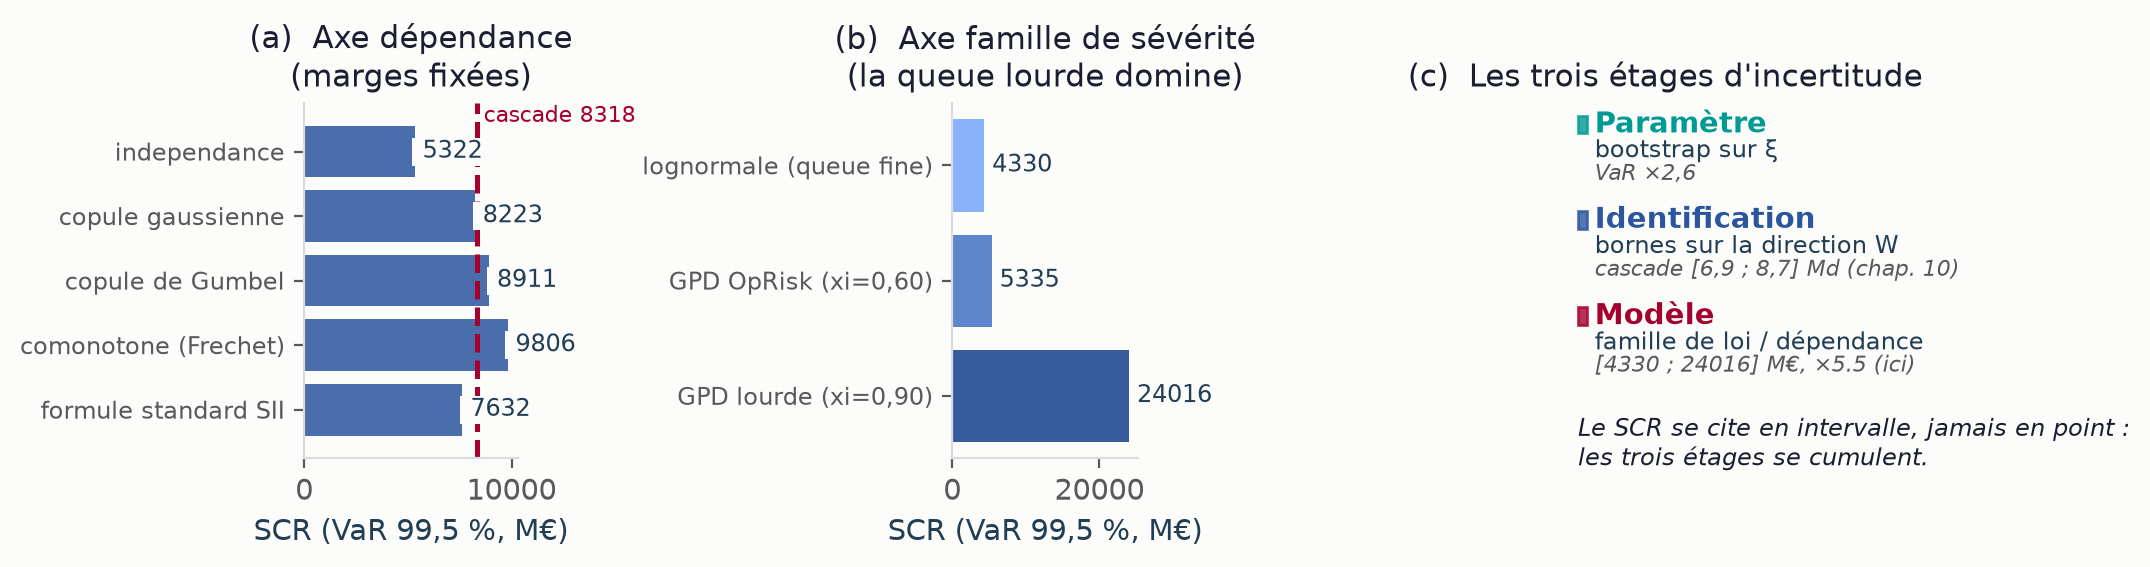
\includegraphics[width=\linewidth]{J4_bande_modele.png}
\caption{La bande de modèle, troisième étage d'incertitude. \textbf{(a)}~axe dépendance, à
marges fixées : la cascade se place entre les copules gaussienne et de Gumbel, dans une bande
$[5{,}3\,;9{,}8]$ Md\euro. \textbf{(b)}~axe famille de queue : la queue lourde domine
l'incertitude ($\times 5{,}5$). \textbf{(c)}~les trois étages (paramètre, identification,
modèle) se cumulent. Source : script~\texttt{48}.}
\label{fig:bande-modele}
\end{figure}

\begin{cle}
\textbf{Oui, chaque brique a des alternatives.} Fréquence (Poisson, Hawkes, Cox), sévérité
(lognormale, splicing, EVT bayésienne), dépendance (copules, réseaux, Hawkes multivarié),
mesure (TVaR, spectrale, robuste), agrégation (formule standard, Panjer) : on ne prétend pas
détenir \emph{la} méthode. La discipline est ailleurs : on a testé les concurrents les plus
sérieux, on \textbf{borne} l'effet du choix, et surtout le niveau bouge dans la bande mais
l'\textbf{ordre d'amorce des piliers ne bouge pas} ($P1>P4>P2>P3>P5$, invariant à la famille).
Le niveau est illustratif, l'ordre résiste : c'est, chiffrée sur un troisième axe, la thèse du
mémoire, et la réponse à qui demanderait \og et si vous aviez pris une autre méthode~?\fg.
\end{cle}

\section{De l'incertitude au chiffre reporté : VaR prédictive et VaR robuste}
\label{sec:predictive-robuste}

Quantifier l'incertitude (les trois étages) ne dit pas encore \emph{quel} nombre reporter.
Prendre le quantile $99{,}5\,\%$ d'une loi estimée en un point (\emph{plug-in}) est fragile,
car les données sont incertaines : \og{}le quantile d'un objet incertain est mauvais\fg{}
(C.~Hillairet). Deux réponses complémentaires, selon la posture (figures~\ref{fig:predictive}
et~\ref{fig:robuste}).

\textbf{La VaR prédictive} intègre l'incertitude de paramètre \emph{avant} de prendre le
quantile : on prend le quantile de la loi \emph{prédictive}, mélange des GPD sur la distribution
bootstrap de $(\xi,\sigma)$. Le résultat est instructif : à $99{,}5\,\%$ elle est \emph{quasi
égale} au \emph{plug-in} ($657$ contre $659$~M\euro) --- le risque d'estimation n'est pas un
biais de point à ce niveau, il ne le devient qu'en profondeur ($+6\,\%$ à $99{,}9\,\%$). La
fragilité est dans la \textbf{largeur} de la bande, pas dans le point.

\textbf{La VaR robuste} prend au contraire la \textbf{borne haute} de la VaR sur l'ensemble
d'ambiguïté (paramètre, puis modèle) : la VaR robuste à $95\,\%$ vaut $1\,026$~M\euro{}
($1{,}6\times$ le \emph{plug-in}), le pire-cas de famille lourde $1\,311$~M\euro. C'est la
posture prudente, où le niveau de robustesse est un \textbf{choix prudentiel explicite}.

\begin{figure}[htbp]\centering
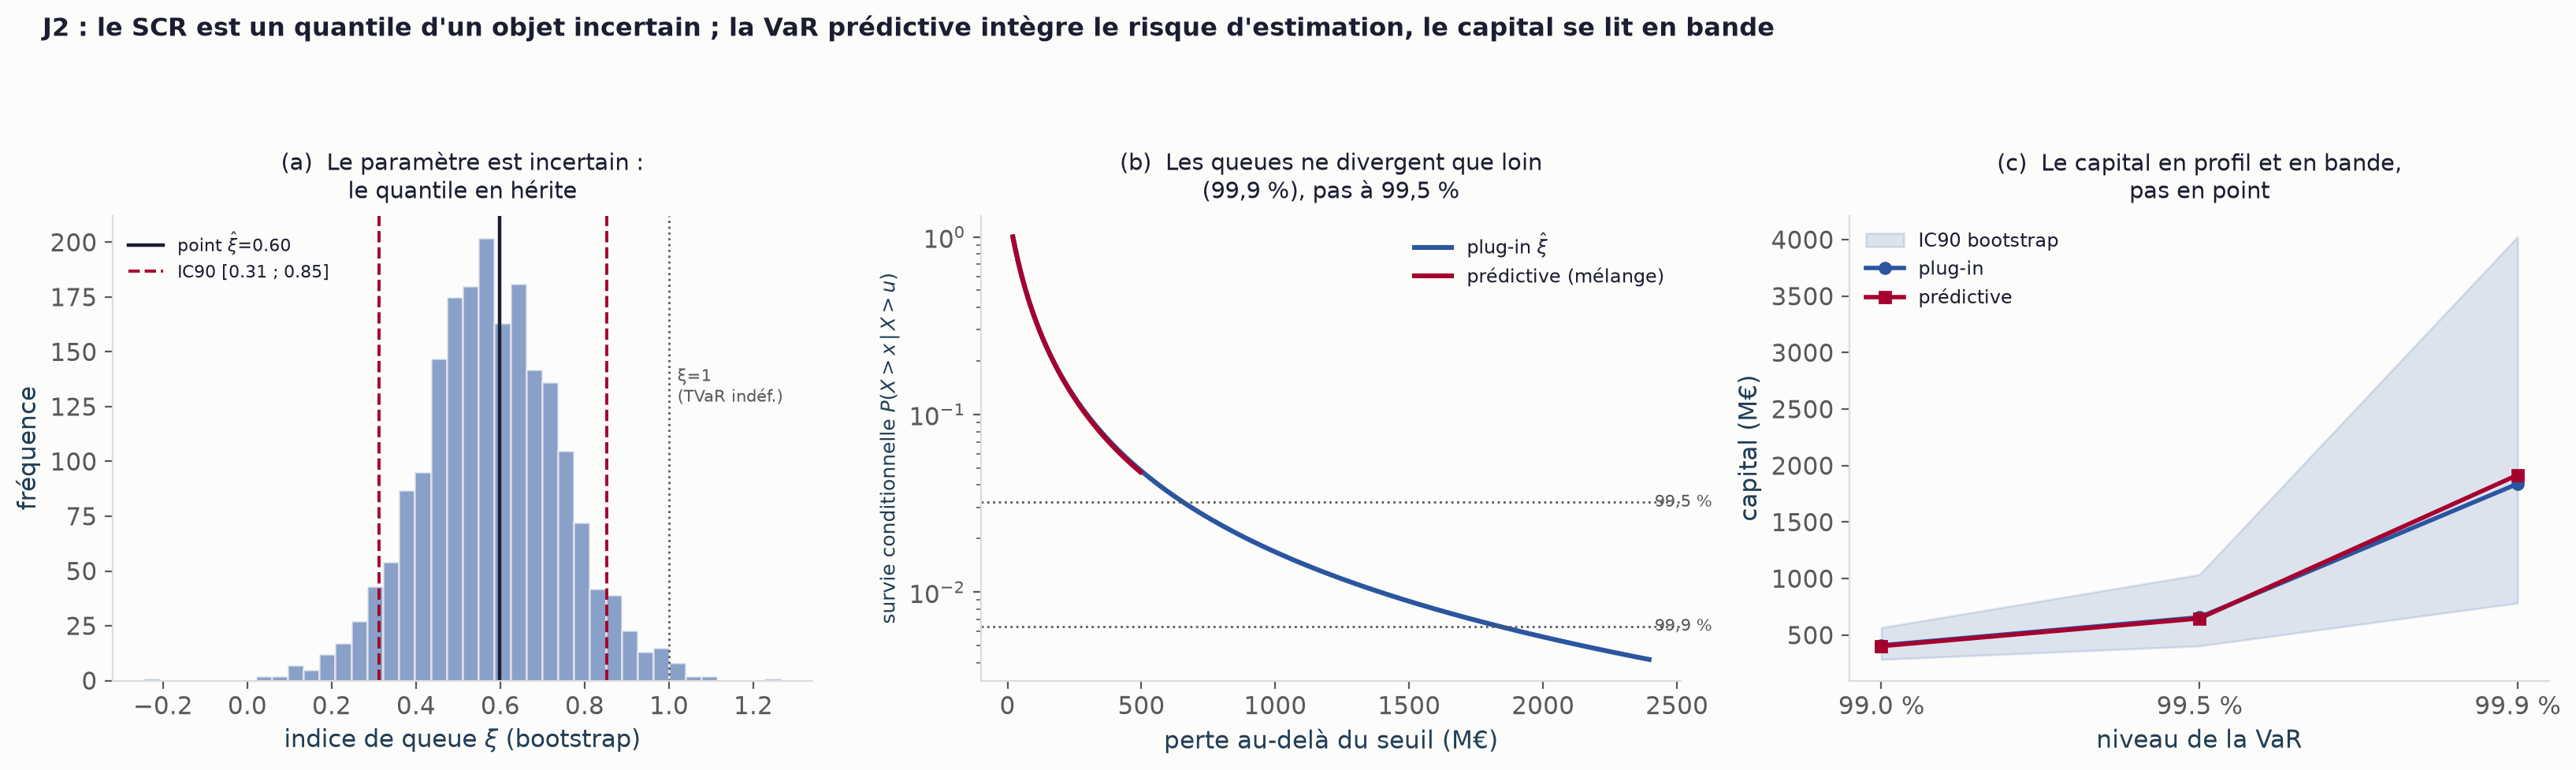
\includegraphics[width=\linewidth]{J2_var_predictive.png}
\caption{VaR prédictive. \textbf{(a)}~le paramètre $\xi$ est incertain. \textbf{(b)}~les queues
\emph{plug-in} et prédictive ne divergent que loin dans la queue. \textbf{(c)}~le capital se lit
en profil et en bande. Source : script~\texttt{46}.}
\label{fig:predictive}
\end{figure}

\begin{figure}[htbp]\centering
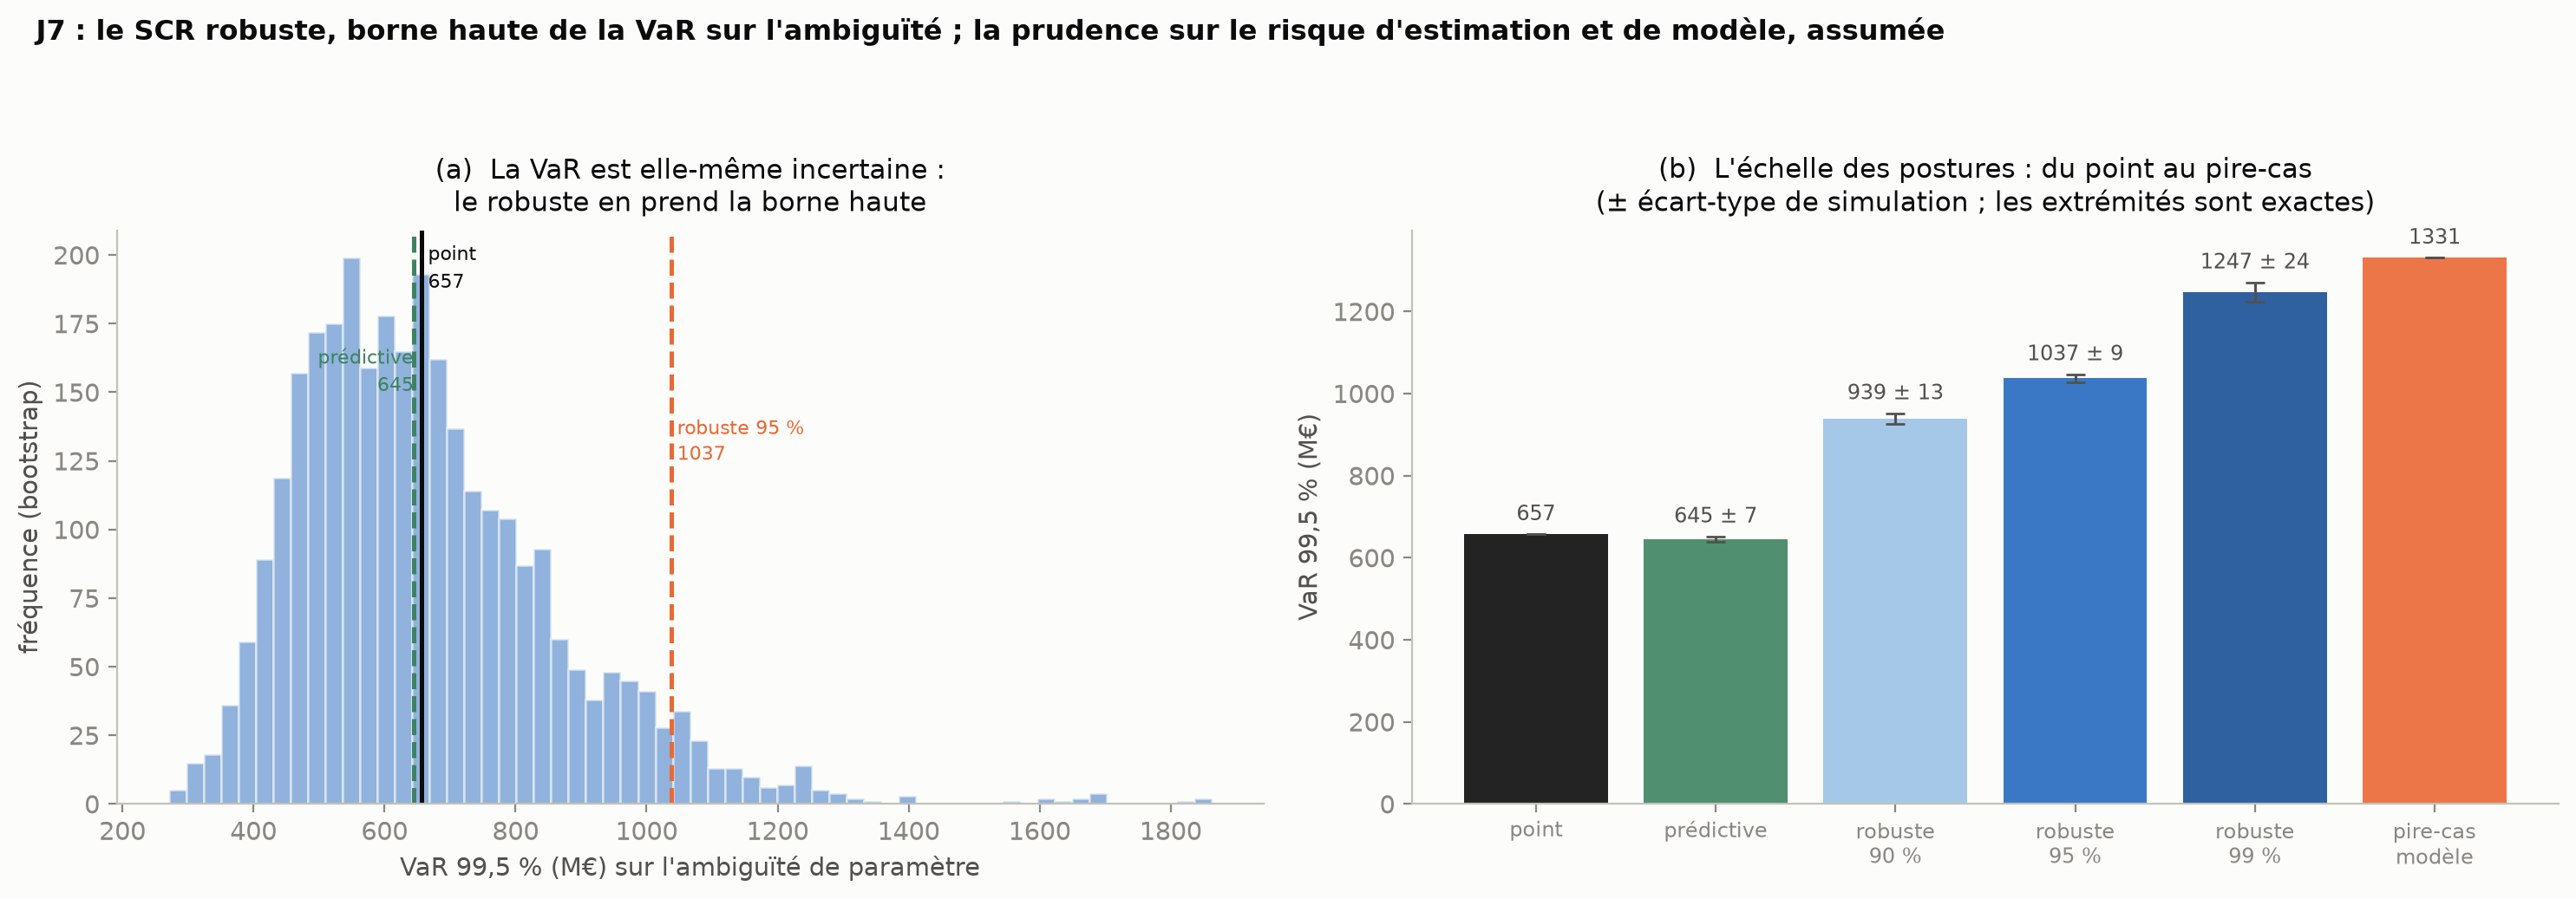
\includegraphics[width=\linewidth]{J7_scr_robuste.png}
\caption{VaR robuste. \textbf{(a)}~la VaR est elle-même incertaine ; le robuste en prend la
borne haute. \textbf{(b)}~l'échelle des postures, du point ($659$) au pire-cas de modèle
($1\,311$~M\euro). Source : script~\texttt{51}.}
\label{fig:robuste}
\end{figure}

\begin{cle}
\textbf{Deux points honnêtes plutôt qu'un point trompeur.} La VaR prédictive est le point
\emph{honnête} (il embarque l'incertitude d'estimation) ; la VaR robuste est le point
\emph{prudent} (la borne haute sur l'ambiguïté). Le choix entre les deux relève de la politique
prudentielle, non du calcul. L'essentiel est de ne jamais reporter le seul \emph{plug-in} : le
SCR se cite avec sa bande, ou par un point qui assume l'incertitude, jamais nu.
\end{cle}

\begin{cle}
\textbf{La double lecture.} \og Insensible aux choix innocents, sensible aux leviers réels \fg :
le modèle n'est ni sur-ajusté ni fragile, il est \textbf{piloté par ce qui doit le piloter}.
Et la seule grande incertitude, la queue, est nommée et bornée, pas cachée. C'est ce qui
transforme \og je n'ai pas tout calibré \fg{} en \og je sais précisément de quoi mon SCR
dépend, et de quoi il ne dépend pas \fg.
\end{cle}

% =====================================================================
        % Hypothèses, sensibilité, étages d'incertitude
\chapter{La donnée manquante comme livrable, hiérarchisé}
\label{ch:livrable}

\begin{cle}
\textbf{Idée directrice.} Le chapitre~\ref{ch:identifiabilite} a montré que la direction de la
contagion n'est pas identifiable sur les sources agrégées. Cette limite n'est pas un point final :
elle se retourne en \textbf{spécification de reporting}, et cette spécification se \textbf{chiffre}
puis se \textbf{hiérarchise}. C'est la contribution réglementaire du travail, et elle ne dépend
d'aucun prior.
\end{cle}

\section{Ce qu'un registre devrait contenir}

Puisque les deux sources agrégées échouent pour des raisons \emph{opposées} (l'une manque de
taxonomie et de volume informatif, l'autre de résolution temporelle), la donnée qui identifierait
$W$ se déduit par complémentarité. Un registre d'incidents \textsc{tic} l'identifiant devrait :
\begin{enumerate}[itemsep=2pt]
\item horodater la \textbf{survenance} (et non la seule déclaration) au \textbf{mois ou à la
      semaine}, afin de porter une antériorité que le pas annuel efface ;
\item catégoriser par \textbf{domaine de contrôle} (les piliers DORA), et non par vecteur
      d'attaque, afin qu'une transition soit interprétable comme un lien $k \to j$ ;
\item consolider une \textbf{cause commune} comme \emph{un} événement à $N$ victimes, pour ne pas
      confondre un lot de déclaration avec une contagion séquentielle.
\end{enumerate}

Ces trois exigences ne sont pas hors d'atteinte : le registre d'information imposé par
l'\emph{implementing technical standard} du règlement d'exécution \citep{eu2024_2956} porte déjà
l'identification des prestataires, la chaîne de sous-traitance et la criticité des fonctions. Ce
qui manque relève du \emph{format} de l'horodatage et du \emph{choix de la taxonomie}, non d'une
collecte nouvelle.

\section{Ce que cette information vaut, en capital}

Une recommandation de reporting reste un v\oe u tant qu'elle n'est pas chiffrée. On la chiffre en
restreignant l'ensemble admissible du chapitre~\ref{chap:partielle} aux configurations compatibles
avec l'information acquise, puis en mesurant le rétrécissement de la bande de capital.

\begin{definition}[Valeur d'information d'une contrainte]\label{def:voi}
Soit $\mathcal{W}$ l'ensemble admissible et $\mathrm{SCR}:\mathcal{W}\to\R_+$ la fonctionnelle de
capital. La largeur de bande associée à un sous-ensemble $\mathcal{V}\subseteq\mathcal{W}$ est
\begin{equation}
  L(\mathcal{V}) \;=\; \sup_{W\in\mathcal{V}}\mathrm{SCR}(W)\;-\;\inf_{W\in\mathcal{V}}\mathrm{SCR}(W).
  \label{eq:largeur-bande}
\end{equation}
Une information $\mathcal{I}$ qui restreint l'ensemble à $\mathcal{W}_{\mathcal{I}}\subseteq
\mathcal{W}$ a pour \textbf{valeur} le rétrécissement relatif qu'elle produit :
\begin{equation}
  V(\mathcal{I}) \;=\; 1-\frac{L(\mathcal{W}_{\mathcal{I}})}{L(\mathcal{W})} \;\in\;[0,1].
  \label{eq:voi}
\end{equation}
\end{definition}

Cette définition a deux propriétés utiles. Elle est \textbf{monotone} : si
$\mathcal{I}'$ implique $\mathcal{I}$, alors $\mathcal{W}_{\mathcal{I}'}\subseteq
\mathcal{W}_{\mathcal{I}}$ et donc $V(\mathcal{I}')\ge V(\mathcal{I})$, une information plus
riche ne pouvant pas valoir moins. Et elle est \textbf{sans dimension}, donc indépendante du
niveau de capital, ce qui la rend comparable d'une source de sévérité à l'autre alors même que
ce niveau, lui, varie d'un facteur quarante.

Le corpus de sept rapports post-incident du chapitre~\ref{ch:identifiabilite} établit le
\emph{sens} de six des dix dépendances entre piliers. À lui seul, il fait tomber la largeur de la
bande de $\mathbf{66\,\%}$. C'est la valeur, en capital, de la lecture de sept documents publics,
et elle donne l'ordre de grandeur de ce qu'un registre correctement spécifié apporterait.

\begin{attention}
\textbf{Ce qu'aucune information de sens ne donnera.} Même les dix directions établies, une bande
subsisterait, imputable à la seule \textbf{amplitude} des coefficients : connaître le sens d'un
lien ne donne pas sa force. L'identification partielle n'est donc pas un état provisoire que la
donnée finirait par lever, elle est \textbf{structurelle}. C'est une raison de plus de lire le
capital en bande, et de ne pas promettre à un superviseur davantage que ce qu'un registre peut
tenir.
\end{attention}

\section{Quelle dépendance documenter en priorité}

L'apport le plus actionnable est ailleurs que dans le total. En fixant le sens d'\emph{une seule}
dépendance à la fois, on obtient un \textbf{classement} des données manquantes par valeur
d'information (figure~\ref{fig:voi}). L'écart est considérable : documenter la seule dépendance
entre gouvernance et gestion des incidents lèverait à elle seule $\mathbf{28{,}9\,\%}$ de
l'ambiguïté de capital, tandis que documenter le lien entre tests et tiers n'en lèverait
\emph{rien}.

Deux conséquences pratiques. D'abord, un superviseur qui ne pourrait exiger qu'une seule
dépendance sait désormais laquelle demander, et une entité qui ne pourrait instrumenter qu'un seul
lien sait lequel instrumenter. Ensuite, un fait qui oriente la recommandation : \textbf{la
dépendance la plus précieuse est précisément celle que le corpus documentaire ne couvre pas}. La
lecture de rapports publics a livré ce qu'elle pouvait livrer ; le reste exige la donnée d'entité.

\begin{figure}[htbp]
\centering
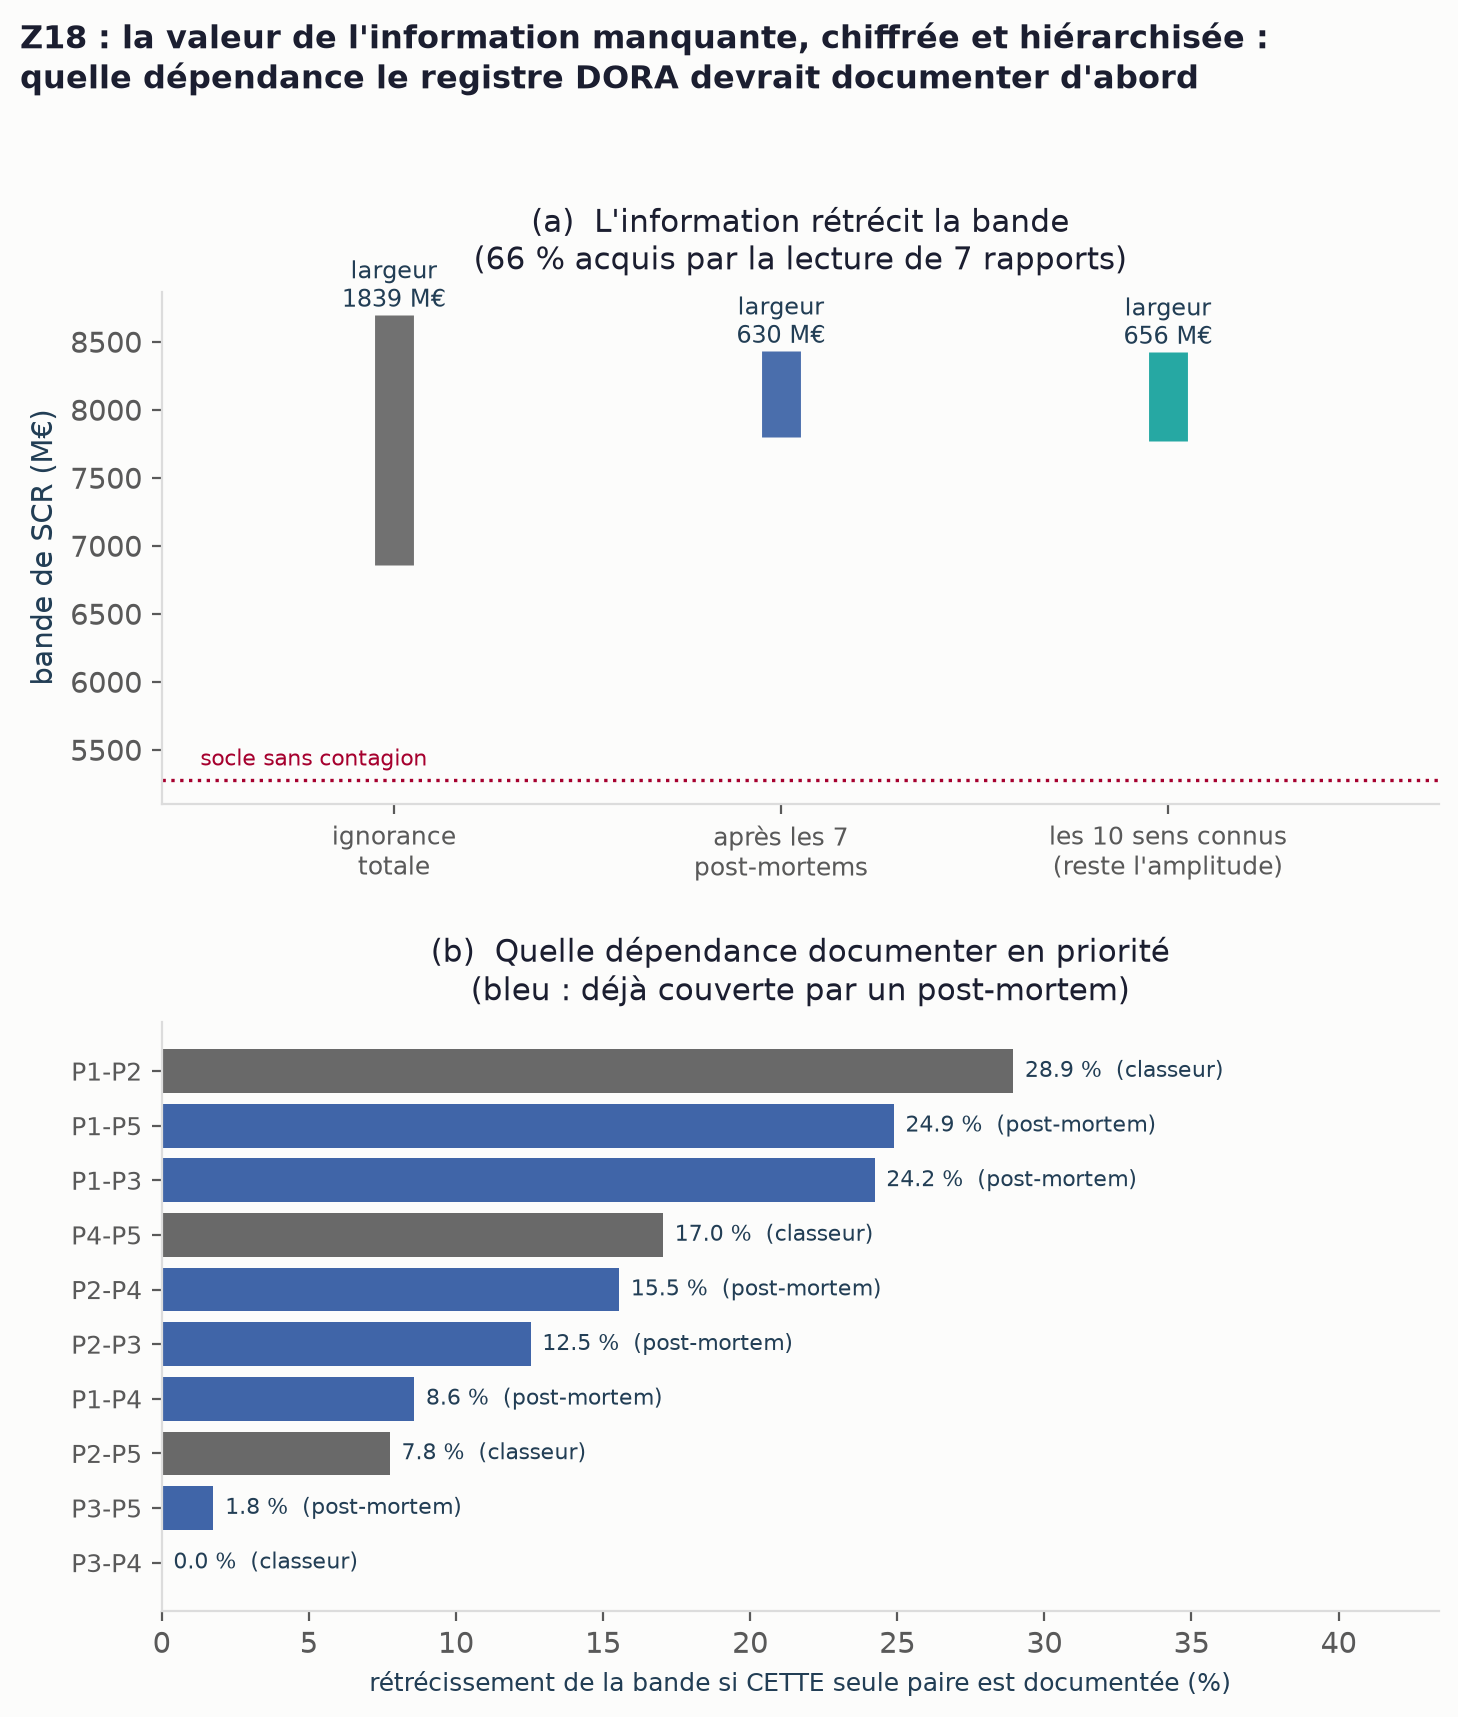
\includegraphics[width=\linewidth]{Z18_valeur_information.png}
\caption{La valeur de l'information, chiffrée et hiérarchisée. (a)~l'information rétrécit la
bande de capital : $66\,\%$ acquis par la lecture de sept rapports, et une bande d'amplitude qui
subsisterait même les dix sens connus. (b)~quelle dépendance documenter en priorité ; en bleu,
celles que le corpus couvre déjà. Source : script~\texttt{55}.}
\label{fig:voi}
\end{figure}

\begin{cle}
\textbf{La limite devenue contribution.} Un mémoire qui se contenterait de constater qu'il ne
peut pas calibrer $W$ laisserait le lecteur sans suite. En spécifiant la donnée qui manque, en
chiffrant ce qu'elle vaut et en la hiérarchisant, on transforme une frontière d'identification en
\textbf{recommandation opposable}, adressée au cadre de reporting que DORA met précisément en
place. C'est le seul endroit du mémoire où une limite produit un livrable.
\end{cle}

% =====================================================================
   % La donnée manquante, chiffrée et hiérarchisée
\chapter{Conclusion}

Ce mémoire a construit un modèle interne partiel du coût en capital de la non-conformité à
DORA, où la dépendance entre les cinq piliers est portée par une cascade dirigée plutôt que
par une copule, et où le capital dépend de l'état de conformité de l'entité. Trois lignes de
résultat s'en dégagent, et ce qui est acquis se dit ici aussi nettement que ce qui
ne l'est pas.

\section{Ce qui est établi}
\paragraph{Le chiffre.} Entre l'état conforme et l'état non conforme sur les quatre canaux, le
besoin de capital passe de $6\,049$ à $20\,188$~M\euro{} à l'échelle du secteur, soit un facteur
$3{,}34$. Les canaux isolés en expliquent $9\,138$~M\euro{} et leur interaction $5\,001$, soit
$35\,\%$ de l'écart : un plan de remédiation doit donc citer l'effet de fermeture d'un canal et
non son effet isolé. La fréquence est le levier qui commande : seule, elle porte le besoin de
capital à $10\,377$~M\euro{}, et toute cible au-delà de $11\,413$~M\euro{} l'exige. Ce montant
reste un besoin de capital au sens de l'ORSA, non un SCR réglementaire.

\paragraph{Le mécanisme.} Le mécanisme tient et se distingue formellement de ses concurrents : la criticité dépend de
l'ordre de propagation, propriété qu'aucune dépendance symétrique ni aucun score
additif ne peut reproduire, et la normalisation de Leontief garantit la stabilité de la
contagion, cycles compris, par construction et non par calibration heureuse. Sur les marges
que la donnée fixe, la queue de sévérité ($\hat\xi = 0{,}5954$ au seuil publié), la
fréquence d'entrée et l'accumulation par cause commune, l'ancrage empirique est solide, et il est
éprouvé hors échantillon : la loi de comptage et la forme de la queue passent le backtest, le
niveau de la charge annuelle ne le passe pas pour une raison mesurée, la dérive de l'échelle de
sévérité. Le processus de Hawkes n'est pas distinguable de la cascade à la résolution
disponible ; il est écarté par un choix de parcimonie argumenté, non par un test qui le
réfuterait. Enfin, le modèle exprime intégralement l'effet de la
conformité sur le capital là où la Formule Standard n'en exprime rien.

\paragraph{Un acquis de méthode, qu'il faut compter comme tel.} Chaque nombre publié dans ce
mémoire est confronté, section par section, aux sorties versionnées des scripts que cette section
cite, et le contrôle rend séparément ce qu'il confirme, ce qu'il exempte avec son motif et ce
qu'il ne confirme pas. Il porte aujourd'hui sur la totalité des nombres du document, sans zone
non couverte autre que celles qui sont déclarées avec leur raison. Ce n'est pas une coulisse
d'atelier : le dispositif a trouvé trois valeurs fausses qu'aucune relecture n'avait vues, toutes
justes au moment où elles avaient été écrites et devenues fausses quand une valeur amont avait
bougé. Il est décrit au \S\ref{sec:ann-harnais}, avec ce qu'il ne garantit pas, car il ne vérifie
ni qu'un nombre est au bon endroit ni qu'il veut dire ce que la phrase prétend.

% SOURCES-SCRIPTS: 28 39 43 68 92 47 89 91 85

\section{Ce qui est démontré comme non mesurable}
La direction de la contagion n'est pas identifiable sur les données publiques. Le
mémoire l'établit sur trois sources qui échouent pour des raisons distinctes, résiste à la
tentation du test dégénéré du temps inversé, et pousse jusqu'à la meilleure expérience
naturelle disponible, le choc de chaîne d'approvisionnement MOVEit, dont l'effet net
s'annule une fois un placebo retranché. Le troisième échec ferme la dernière échappatoire :
le schéma \textsc{veris}, standard de description d'incidents adopté par la profession, porte
littéralement les deux champs manquants, et leur intersection n'est renseignée que dans
\emph{un} incident sur $10\,591$. Le problème n'est donc pas de savoir quoi collecter, il est
d'en rendre le remplissage obligatoire. Cette limite n'est pas dissimulée, elle est
convertie en méthode : le capital est borné sur l'ensemble des matrices admissibles plutôt
qu'appuyé sur une matrice posée. Le socle sans contagion est ainsi défendable sans aucune hypothèse non
identifiable, et la contagion ajoute une bande explicite au-dessus de ce socle.

% SOURCES-SCRIPTS: 30 34 28

\section{Ce qui en découle pour le régulateur}
La donnée qui rendrait la contagion mesurable se déduit par complémentarité des trois échecs :
un registre d'incidents horodatant la survenance à la semaine, catégorisant par
domaine de contrôle et non par vecteur d'attaque, consolidant une cause commune
comme un événement unique, et consignant l'ensemble des piliers touchés par chaque incident,
dont la loi jointe distingue à elle seule une matrice de sa transposée. Les deux premières exigences sont déjà des champs normalisés du
schéma \textsc{veris} : la recommandation ne demande donc pas d'inventer une taxonomie, elle
demande d'en rendre le remplissage obligatoire, ce que la notification d'incident
majeur sous DORA peut imposer et qu'une base déclarative volontaire ne peut pas. Cette
spécification n'est pas un v\oe{}u : le mémoire chiffre en euros de capital le resserrement des
bornes qu'elle apporterait, et la hiérarchise par dépendance. La limite d'identifiabilité
devient une recommandation de reporting opposable, ce qui donne au travail une portée
au-delà du modèle.

\section{Ce qui en découle pour l'entité}
Le capital n'est pas seulement un chiffre à publier, c'est un coût. En le confrontant au prix
de marché du même risque, le mémoire met les trois leviers d'une entité, remédier, détenir,
transférer, sur un seul axe en euros par an. À l'échelle d'entité, le coût annuel de détention
vaut plus de deux fois la sinistralité attendue, un traité en excès de perte correctement
dimensionné réduit le coût total d'au plus deux tiers environ, borne supérieure que la capacité
du marché, les exclusions et le risque de contrepartie entament, et la remédiation déplace ce point
d'équilibre en plus d'abaisser le capital. Le niveau reste illustratif, et il l'est doublement
puisque la descente d'échelle du secteur vers l'entité passe par deux élasticités estimées.
Mais le \emph{rapport} entre coût de détention et prix de transfert résiste mieux que le
niveau, et pour une raison qui est une identité plutôt qu'une mesure : ses deux termes
sont proportionnels au \emph{même} SCR, qui se simplifie, de sorte qu'un changement d'échelle
pur le laisse inchangé. Il vaut $2{,}78$ au taux de la directive et $3{,}51$ au taux
historique. Ce qui subsiste est un effet de forme, la descente d'échelle déplaçant la
fréquence et la sévérité séparément plutôt que de redimensionner la loi de perte, et le seul
balayage disponible le borne par le haut à $+36\,\%$ sur une plage de SCR d'un facteur quatre.
C'est la lecture décisionnelle que le travail visait, et elle est plus robuste que le niveau
sans être invariante.

% SOURCES-SCRIPTS: 58 65 67

\section{Limites, sans détour}
L'élicitation structurée est préparée et non exécutée (annexe~\ref{ch:elicitation}) : la
lecture centrale de la direction repose donc sur un classeur qualitatif, non sur une agrégation
d'experts pondérée. Deux hypothèses pèsent le plus sans être testables sur la donnée : les
niveaux de propagation, posés, et l'additivité des coûts entre piliers touchés, dont
l'élasticité vaut $0{,}95$ à l'état non conforme contre $0{,}39$ à l'état conforme
(\S\ref{sec:additivite-couts}). Dans les deux cas le signe et l'ordre de l'écart résistent à
toute la plage étudiée, non son amplitude. Le
niveau absolu du SCR est illustratif et ne doit pas être cité hors de son cadrage relatif.
L'incertitude de queue domine toute lecture ponctuelle, ce qui impose de présenter le capital
en distribution. Et l'ordre de remédiation entre les deux piliers de tête, la gouvernance et
la gestion des tiers, dépend de la direction non identifiée : le mémoire sait dire que ces
deux-là dominent, pas lequel remédier d'abord sans un dire d'expert.

% SOURCES-SCRIPTS: 74

\section{Ouvertures}
Trois prolongements se dessinent : mener l'élicitation structurée pour resserrer la bande
directionnelle sur ses deux degrés de liberté restants ; approfondir le pilier des tiers sur
des données clients, là où l'open data s'effondre ; et passer de la sensibilité de
propagation à une véritable criticité au sens de l'audit, c'est-à-dire au risque résiduel
après mesures de contrôle, une fois disponible une métrique de mitigation par pilier.

% =====================================================================
                   % Conclusion

% =====================================================================
\appendix
% PAS DE \addcontentsline ICI, ET C'EST LA SEULE DIVERGENCE DE FOND AVEC main.tex.
% preambule_v2 redefinit \part par titlesec en style [display], et dans cette
% configuration titlesec ecrit LUI-MEME l'entree de sommaire d'un \part*. La ligne
% explicite que porte main.tex, indispensable la puisque \part* n'y ecrit rien, en
% ajoutait donc une SECONDE ici : le sommaire de la v2 portait << Annexes >> deux
% fois, aux pages 141 et 142, depuis la creation de la v2 le 8 septembre 2026.
% Defaut trouve le 9 septembre en comparant les deux .toc, et corrige ici plutot
% que dans le preambule : desactiver l'ecriture de titlesec toucherait les cinq
% \part numerotes, qui, eux, s'inscrivent correctement.
\part*{Annexes}

% -----------------------------------------------------------------------------
% NOTICE D'ORGANISATION DES ANNEXES. Les annexes B (demonstrations du socle EVT),
% D (pieces justificatives) et E (complements aux chapitres du corps) ont ete
% deportees le 18 septembre 2026 vers materiel_complementaire/ et ne sont plus
% appelees. Leurs 78 etiquettes sont donc mortes : tous les renvois du corps qui
% pointaient vers elles ont ete remplaces par la macro \matcomp, definie dans
% preambule_v2.tex. Ne pas remettre un \ref vers ces etiquettes.
% -----------------------------------------------------------------------------
\chapter*{Organisation des annexes et matériel complémentaire}
\addcontentsline{toc}{chapter}{Organisation des annexes et matériel complémentaire}

Afin de faciliter la lecture de ce mémoire, seules les démonstrations de la contribution
principale (le modèle de cascade), les adaptations spécifiques aux piliers \textsc{dora},
ainsi que le protocole d'élicitation et ses retours de praticiens sont inclus dans ce
document.

L'ensemble du \textbf{matériel complémentaire}, comprenant les démonstrations des théorèmes
standards des valeurs extrêmes, les pièces justificatives et les diagnostics de robustesse,
ainsi que les compléments de chapitres, a été déporté dans un dépôt numérique pérenne.

Il est consultable et téléchargeable à l'adresse suivante :
\url{https://LIEN_VERS_LE_DEPOT.com}

% =====================================================================
\chapter{Démonstrations : le modèle de cascade}
\label{ann:cascade}

% HARNAIS-HORS-SCRIPT: chapitre de demonstrations de la cascade : memes constantes d'enonce ; les valeurs numeriques correspondantes sont verifiees au chapitre cascade, qui cite ses scripts.

Cette annexe démontre les propriétés énoncées à la section~\ref{sec:formalisation}. Les
notations sont celles du chapitre~\ref{chap:cascade} : $P=\{1,\dots,5\}$, $W\in[0,1]^{P\times P}$
avec $W_{jj}=0$, et la cascade indépendante de la définition~\ref{def:cascade}.

\section*{Forme réduite et descendance espérée (proposition~\ref{prop:reduite})}

\begin{proof}
Soit $\mathcal M_n(a,k)$ le nombre de marches dirigées de longueur $n$ de $a$ vers $k$ dans le
graphe pondéré. Une marche $a=v_0\to v_1\to\cdots\to v_n=k$ est vivante avec probabilité
$\prod_{t} W_{v_{t-1}v_t}$, ces arêtes étant indépendantes ; en sommant sur les marches,
$\mathbb E\,\mathcal M_n(a,k)=\sum \prod_t W_{v_{t-1}v_t}=(W^n)_{ak}$ par définition du produit
matriciel. Le nombre de fois où $k$ est atteint depuis $a$ en comptant \emph{chaque} chemin
vaut $\sum_{n\ge0}\mathcal M_n(a,k)$, d'espérance $\sum_{n\ge0}(W^n)_{ak}$. Cette série
matricielle est la série de Neumann de $W$ ; elle converge vers $(I-W)^{-1}$ si et seulement si
$\rho(W)<1$, auquel cas $\sum_{n\ge0}W^n=(I-W)^{-1}$.

L'indicatrice $\mathbf 1\{k\in S_a\}$ vaut $1$ dès qu'\emph{au moins un} chemin vivant relie
$a$ à $k$, donc $\mathbf 1\{k\in S_a\}\le \sum_{n\ge0}\mathcal M_n(a,k)$ presque sûrement. En
prenant l'espérance puis en sommant sur $k$,
\[
  \mathbb E\,|S_a|=\sum_k \mathbb P(k\in S_a)\le \sum_k\bigl((I-W)^{-1}\bigr)_{ak}
  =\bigl[(I-W)^{-1}\mathbf 1\bigr]_a .
\]
L'inégalité est stricte dès qu'un pilier est accessible par plusieurs chemins avec probabilité
positive, ce qui quantifie les collisions.
\end{proof}

\section*{Sous-criticité par normalisation (proposition~\ref{prop:leontief})}

\begin{proof}
Par construction~\eqref{eq:norm}, $W=(g/s_{\max})\,\mathrm{TRANS}\ge 0$ et, pour toute ligne
$j$, $\sum_k W_{jk}=(g/s_{\max})\sum_k \mathrm{TRANS}_{jk}\le (g/s_{\max})\,s_{\max}=g$, puisque
$s_{\max}$ est la plus grande somme de ligne de $\mathrm{TRANS}$. Pour une matrice à
coefficients positifs, le rayon spectral est majoré par toute norme d'opérateur subordonnée,
en particulier la norme infinie, qui est le maximum des sommes de lignes :
$\rho(W)\le\lVert W\rVert_\infty=\max_j\sum_k W_{jk}\le g<1$. La série de Neumann converge donc
et $(I-W)^{-1}=\sum_{n\ge0}W^n$ existe, à coefficients positifs.
\end{proof}

\section*{Loi exacte de l'ensemble atteint (proposition~\ref{prop:loi})}

\begin{proof}
Fixons $A\ni a$. L'événement $\{S_a=A\}$ est l'intersection de deux événements portant sur des
arêtes disjointes, donc indépendants : (i) aucune arête ne relie $A$ à son complémentaire (sans
quoi $S_a$ dépasserait $A$), et (ii) $a$ atteint tout $A$ par les seules arêtes internes à $A$.
L'événement (i) ne concerne que les arêtes $j\to k$ avec $j\in A$, $k\notin A$, chacune absente
avec probabilité $1-W_{jk}$ indépendamment ; sa probabilité est $B(A)=\prod_{j\in A,k\notin A}(1-W_{jk})$.
L'événement (ii) ne concerne que les arêtes internes à $A$ ; notons $R(A)$ sa probabilité.
Par indépendance, $\mathbb P(S_a=A)=R(A)\,B(A)$.

Pour $R(A)$, on partitionne selon le sous-ensemble $A'$ effectivement atteint par les arêtes
internes : $A'$ contient $a$, et $A'\subsetneq A$ est \emph{propre} si et seulement si $A$
n'est pas entièrement atteint. Or, conditionnellement à ce que l'ensemble atteint par les
arêtes internes soit exactement $A'$, aucune arête ne va de $A'$ vers $A\setminus A'$, événement
de probabilité $\prod_{j\in A',k\in A\setminus A'}(1-W_{jk})$ et indépendant de la réalisation
interne à $A'$. En sommant les probabilités de ces sous-ensembles propres et en passant au
complémentaire,
\[
  R(A)=1-\sum_{\substack{A'\subsetneq A\\ a\in A'}} R(A')\!\!\prod_{j\in A',k\in A\setminus A'}\!\!(1-W_{jk}),
\]
avec $R(\{a\})=1$. La récursion sur les sous-ensembles emboîtés est finie et détermine $R$ de
proche en proche.
\end{proof}

\section*{Monotonie stochastique (proposition~\ref{prop:mono})}

\begin{proof}
On construit un \emph{couplage}. Soit $(U_{jk})$ une famille de variables uniformes sur $[0,1]$
indépendantes, commune aux deux matrices. Pour une matrice $M$, déclarons l'arête $j\to k$
vivante si $U_{jk}<M_{jk}$ ; le graphe obtenu a la bonne loi (arête vivante avec probabilité
$M_{jk}$). Si $W\le W'$ terme à terme, alors $U_{jk}<W_{jk}\Rightarrow U_{jk}<W'_{jk}$ : toute
arête vivante sous $W$ l'est sous $W'$. Le graphe sous $W$ est donc un sous-graphe de celui sous
$W'$, et l'accessibilité étant croissante par ajout d'arêtes, $S_a(W)\subseteq S_a(W')$ presque
sûrement. Pour toute fonctionnelle $\varphi$ croissante pour l'inclusion,
$\varphi(S_a(W))\le\varphi(S_a(W'))$ p.s., d'où la domination stochastique et la monotonie de
l'espérance et des quantiles. Enfin, pour une perturbation antisymétrique $A$, l'entrée $W_{jk}$
croît quand $W_{kj}$ décroît : les deux effets jouent en sens contraire sur $S_a$, la monotonie
en $A_{jk}$ n'a plus lieu, et l'optimum sur le pavé $\{|A_{jk}|\le t\,S_{jk}\}$ doit être
cherché aux sommets sans garantie qu'ils le réalisent.
\end{proof}

\section*{Dépendance à l'ordre et non-identification (propositions~\ref{prop:ordre} et~\ref{prop:nonid})}

\begin{proof}
\emph{Ordre.} Soit $\sigma=(i_1,\dots,i_n)$ et $\sigma'$ une permutation de $\sigma$. Alors
$\ell(\sigma)=\ell(\sigma')$ pour toute paire si et seulement si le produit
$\prod_k \mathrm{TRANS}_{i_k i_{k+1}}$ ne dépend pas de l'ordre des facteurs disponibles, ce qui,
pour $n=2$, équivaut à $\mathrm{TRANS}_{ij}=\mathrm{TRANS}_{ji}$ pour tout $(i,j)$, soit la
symétrie de $\mathrm{TRANS}$. La contraposée donne le résultat : $\mathrm{TRANS}$ asymétrique
implique l'existence d'une paire dont l'ordre change la vraisemblance, donc la criticité n'est
pas une fonction de l'ensemble. Toute copule et tout score additif étant symétriques en leurs
arguments, aucun ne reproduit cette dépendance.

\emph{Non-identification.} La décomposition $W=\tfrac12(W+W^\top)+\tfrac12(W-W^\top)=S+A$ est
unique car $S$ est symétrique, $A$ antisymétrique, et cette somme directe est celle des
matrices en parties symétrique et antisymétrique. La co-occurrence observée d'une paire
$\{j,k\}$ est, par échange des rôles, une fonction de $W_{jk}+W_{kj}=2S_{jk}$ seulement ; de
même la statistique d'asymétrie du placebo compare $M$ à sa transposée et son espérance sous
permutation ne dépend que de $S$. Donc $W$ et $W^\top=S-A$ induisent les mêmes lois observables
de co-occurrence. Ils diffèrent par le signe de $A$, et la proposition~\ref{prop:mono} montre
qu'un tel changement modifie l'ensemble atteint, donc le SCR, en général : la direction est non
identifiée.
\end{proof}

\section*{Efficience de la valeur de Shapley}
\label{sec:ann-efficience-shapley}

Le chapitre~\ref{chap:resultats} attribue le surcoût de capital aux piliers par la valeur de
Shapley, et lit dans le tableau que la colonne des parts somme exactement à cent. Cette somme
n'est ni une coïncidence ni un artefact d'arrondi : c'est la propriété d'\textbf{efficience}
\citep{Shapley1953}, et elle se démontre en quelques lignes. Elle est reproduite ici parce que
c'est elle, et elle seule, qui autorise à présenter une attribution comme une \emph{partition} du
surcoût et non comme une pondération arbitraire.

\begin{proposition}[Efficience]
\label{prop:efficience}
Soit $v$ une fonction caractéristique sur $\{1,\dots,n\}$ avec $v(\emptyset)=0$, et
\[
  \varphi_i \;=\; \frac1n \sum_{u \subseteq -\{i\}} \binom{n-1}{|u|}^{-1}
                  \bigl[v(u \cup \{i\}) - v(u)\bigr].
\]
Alors $\sum_{i=1}^{n} \varphi_i = v(\{1,\dots,n\})$.
\end{proposition}

\begin{proof}
La démonstration repose entièrement sur la réécriture du poids. Pour $|u|=s$,
\begin{equation}
  \frac1n \binom{n-1}{s}^{-1} \;=\; \frac1n \cdot \frac{s!\,(n-1-s)!}{(n-1)!}
  \;=\; \frac{s!\,(n-s-1)!}{n!},
  \label{eq:poids-shapley}
\end{equation}
de sorte que $\varphi_i$ est exactement la moyenne, sur les $n!$ \textbf{permutations} de
$\{1,\dots,n\}$, de la contribution marginale de $i$ à l'ensemble de ses prédécesseurs. En effet,
un sous-ensemble $u$ de cardinal $s$ ne contenant pas $i$ est l'ensemble des prédécesseurs de $i$
dans exactement $s!\,(n-s-1)!$ permutations : $s!$ ordres pour les éléments de $u$, puis
$(n-s-1)!$ pour ceux qui suivent $i$. En notant $\Pi$ l'ensemble des permutations et $P_i(\pi)$
les prédécesseurs de $i$ dans $\pi$,
\[
  \varphi_i \;=\; \frac{1}{n!} \sum_{\pi \in \Pi}
              \bigl[v\bigl(P_i(\pi) \cup \{i\}\bigr) - v\bigl(P_i(\pi)\bigr)\bigr].
\]
Sommons alors sur $i$ \emph{à permutation fixée}. Si $\pi = (\pi(1),\dots,\pi(n))$, les
ensembles de prédécesseurs emboîtés donnent
$P_{\pi(j+1)}(\pi) = P_{\pi(j)}(\pi) \cup \{\pi(j)\}$, si bien que la somme des contributions
marginales le long de $\pi$ est \textbf{télescopique} :
\[
  \sum_{i=1}^{n} \bigl[v\bigl(P_i(\pi)\cup\{i\}\bigr)-v\bigl(P_i(\pi)\bigr)\bigr]
  \;=\; \sum_{j=1}^{n} \bigl[v\bigl(P_{\pi(j+1)}(\pi)\bigr)-v\bigl(P_{\pi(j)}(\pi)\bigr)\bigr]
  \;=\; v(\{1,\dots,n\}) - v(\emptyset),
\]
et cette valeur ne dépend pas de $\pi$. En moyennant sur les $n!$ permutations,
$\sum_i \varphi_i = v(\{1,\dots,n\})$, puisque $v(\emptyset)=0$.
\end{proof}

\paragraph{Ce que l'efficience garantit, et ce qu'elle ne garantit pas.}
Elle garantit que l'attribution est une partition \emph{exacte} du surcoût, quelle que soit
l'interaction et quel que soit son signe : rien n'est perdu ni dupliqué. Elle ne garantit
\textbf{pas} que la part d'un joueur soit une prédiction de ce qu'on obtiendrait en l'écartant
seul, laquelle est la contribution \emph{marginale} et ne somme pas au total. C'est la distinction
que le chapitre~\ref{chap:resultats} tient entre les trois lectures d'un même canal, et l'annexe
des adaptations par pilier en donne l'identité correspondante pour chaque colonne. En particulier,
une part de Shapley est une \emph{convention} d'attribution défendable, non un budget de
remédiation : deux des quatre canaux du modèle sont bornés et non calibrés.

\paragraph{Pourquoi aucun échantillonnage n'est nécessaire ici.}
La réécriture~\eqref{eq:poids-shapley} est aussi ce qui rend le calcul praticable : elle ramène
l'évaluation à une moyenne sur les permutations, forme sur laquelle reposent les algorithmes
d'approximation en temps polynomial \citep{CastroGomezTejada2009, SongNelsonStaum2016},
indispensables dès que la dimension croît. Avec cinq piliers, les $5!$ permutations et les $2^5$
valeurs de $v$ sont énumérées exhaustivement : les valeurs publiées sont donc exactes au bruit de
simulation de $v$ près, et aucune erreur d'approximation combinatoire ne s'y ajoute.

  % Démonstrations : cascade
\chapter{Adaptations par pilier}
\label{chap:adaptations}

\begin{cle}
\textbf{Idée directrice, et statut de cette annexe.} Le modèle fait passer le Vasicek d'un
facteur unique à un facteur \emph{par pilier}. Les autres composants doivent-ils suivre ? Les
cinq piliers ne sont pas cinq exemplaires du même risque : la queue de sévérité,
l'accumulation par tiers et la détection sont des objets de nature différente. Cette annexe
les adapte pilier par pilier, sous la \emph{même} discipline que le
chapitre~\ref{chap:partielle} : on n'adopte un raffinement que si la donnée le soutient, et
ce qu'elle ne fixe pas, on le borne. Elle est reportée hors du corps parce que son
verdict est constant et ne modifie aucune conclusion : chaque adaptation relève le
niveau, aucune ne renverse le classement.
\end{cle}

\section{La queue de sévérité par pilier}
\label{sec:xi-pilier}

Aujourd'hui une seule queue $\xi$ est appliquée aux cinq piliers. Le
chapitre~\ref{chap:donnees} note pourtant que la queue est hétérogène selon la catégorie
Bâle : $\xi$ varie de $0{,}87$ (\emph{Employment}) à $1{,}37$ (\emph{Execution, Delivery \&
Process Management}), soit une dispersion de $0{,}50$, sur une table recalculée pour ce mémoire.
% SOURCES-SCRIPTS: 67
Faut-il un $\xi_j$ par pilier ? La réponse distingue deux choses.

\begin{attention}
\textbf{L'hétérogénéité est un fait, l'assignation n'en est pas un.} On ne peut pas
\emph{poser} $\xi_j = f(\text{pilier})$ : les catégories Bâle décrivent la nature de la
perte, pas les domaines de contrôle DORA, et la catégorie la plus proche du TIC
(\emph{Business Disruption \& System Failures}) n'a que $111$ observations, sous le seuil
d'estimation de $150$. On applique donc la logique du chapitre~\ref{chap:partielle} : chaque pilier
reçoit une des cinq queues observées, on énumère les $120$ assignations, et l'on borne le
SCR. Pour isoler l'hétérogénéité du niveau, les cinq queues sont centrées sur la valeur de
référence.
\end{attention}

Le résultat est net, et en partie inattendu. L'hétérogénéité de queue n'est pas
neutre en capital : même en gardant la moyenne des queues fixe, donner à chaque pilier sa
propre queue relève le SCR de $+55\,\%$ à $+96\,\%$. C'est un effet de convexité, la
VaR croissant plus vite que linéairement en $\xi$, de sorte qu'une queue lourde sur un pilier
n'est pas compensée par une queue légère ailleurs. Supposer une queue commune
sous-estime donc le capital, une raison de plus de lire le niveau en bande. Le classement,
lui, résiste : le pilier de tête reste dominant dans $83\,\%$ des assignations
(figure~\ref{fig:xi-pilier}), dominant sans être invariant.

\begin{figure}[htbp]\centering
\figover{Z8_xi_par_pilier.png}
\caption{Queue de sévérité par pilier. (a)~Le niveau du SCR borné sur les $120$ assignations
des queues observées aux piliers ; une queue commune (trait) est en bas de la bande.
(b)~Le pilier de tête par contribution à la queue ne dépend pas de l'assignation.}
% SOURCES-SCRIPTS: 37
\label{fig:xi-pilier}
\end{figure}

\section{Le pilier des tiers comme n\oe{}ud d'accumulation}
\label{sec:p4-accumulation}

P4 (prestataires tiers) n'est pas un n\oe{}ud de cascade comme les autres. Une défaillance
d'un prestataire \emph{partagé} dégrade plusieurs piliers simultanément, par
dépendance commune, au lieu de se propager de proche en proche : c'est le mécanisme de MOVEit
($191$ victimes d'un seul choc, chapitre~\ref{chap:donnees}). On lui
% SOURCES-SCRIPTS: 08g
substitue donc un
\emph{choc commun}, où P4 et chaque autre pilier tombent ensemble avec une probabilité
$\varphi_{cs}$, plutôt qu'une propagation dirigée.

\begin{cle}
\textbf{Pourquoi P4 échappe à la limite d'identification de $W$.} Le choc commun est une
\emph{co-occurrence symétrique} : P4 et $P_j$ tombent ensemble, sans direction. Or la
co-occurrence est la partie \emph{identifiée} du modèle, le $S$ de la décomposition
$W=S+A$ (chapitre~\ref{chap:partielle}), celle que la donnée voit (MOVEit, concentration
cloud). L'accumulation de P4 est donc la seule structure inter-piliers que la donnée
soutient, par contraste avec la direction, non identifiée. C'est un point de force, pas une
limite.
\end{cle}

L'intensité $\varphi_{cs}$ au sein d'une entité isolée n'est pas identifiée (le \emph{batch}
observé est un phénomène de portefeuille) : on la borne sur $[0,\gamma]$, où $\gamma=0{,}68$
est la concentration cloud déjà retenue. Le SCR se lit alors en bande, et à
$\varphi_{cs}=\gamma$ une dépendance partagée emporte en moyenne $3{,}7$ piliers d'un coup,
soit $+19\,\%$ de SCR par rapport au traitement en n\oe{}ud de cascade. Surtout, la
simultanéité crée une co-occurrence multiple que la propagation séquentielle ne produit
presque jamais : la probabilité qu'un incident P4 touche au moins trois piliers passe de
$0{,}22$ (cascade) à $0{,}90$ (choc commun), figure~\ref{fig:p4}.

\begin{figure}[htbp]\centering
\figover{Z9_p4_accumulation.png}
\caption{Le pilier des tiers en accumulation. (a)~SCR borné sur l'intensité du choc partagé
$\varphi_{cs}\in[0,\gamma]$, comparé au traitement de P4 en n\oe{}ud de cascade (trait).
(b)~La simultanéité crée une co-occurrence multiple, structure symétrique donc identifiée.
}
% SOURCES-SCRIPTS: 38
\label{fig:p4}
\end{figure}

\subsection{Le seuil de déclenchement, et l'accumulation bornée par la dépendance de queue}
\label{sec:p4-seuil}

Il faut séparer deux questions, celle de la \emph{marge} et celle de la \emph{dépendance}.

\paragraph{La marge : quand un pilier bascule.} Le déclenchement est un franchissement,
\begin{equation}
  \{\text{pilier } j \text{ déclenché}\} \;=\; \{X_j \ge K_j\},
  \qquad K_j = F^{-1}(1-p_j),
  \label{eq:seuil-Kj}
\end{equation}
et pour $P_4$, $p_4=0{,}151$ donne $K_4=1{,}03$. La loi $F$ de la latente n'y est qu'une
\emph{normalisation} : par construction $\Prob(X_j\ge K_j)=p_j$ \emph{quelle que soit} $F$
continue et strictement croissante, de sorte que le choix de $F$ ne transporte aucune information
sur la fréquence de déclenchement. La queue lourde du capital vit dans la sévérité (GPD,
chapitre~\ref{chap:socle}), non dans ce seuil : une loi normale y est donc inoffensive.

\paragraph{La dépendance : combien de piliers ensemble.} L'accumulation, elle, est gouvernée par
la dépendance de queue supérieure de la copule $C$ liant les latentes,
\begin{equation}
  \lambda_U \;=\; \lim_{u\to 1^-}\Prob\bigl(U_2>u \,\big|\, U_1>u\bigr)
             \;=\; \lim_{u\to 1^-}\frac{1-2u+C(u,u)}{1-u} .
  \label{eq:lambda-U}
\end{equation}
Une copule gaussienne vérifie $\lambda_U=0$ quelle que soit sa corrélation, tandis que la copule
de Gumbel de paramètre $\theta>1$ donne
\begin{equation}
  \lambda_U^{\text{Gumbel}} \;=\; 2-2^{1/\theta},
  \label{eq:lambda-gumbel}
\end{equation}
soit $0{,}53$ pour le $\theta=1{,}8$ retenu ailleurs dans le mémoire. Retenir une copule
gaussienne ici sous-estimerait donc structurellement le co-extrême, en contradiction avec ce
choix.

\begin{attention}
\textbf{Borner l'accumulation, à dépendance moyenne égale.} On ne tranche pas la copule : on
lit le co-déclenchement en bande, à $\tau$ de Kendall égal, entre le plancher gaussien
et le haut de Gumbel. La fréquence \emph{marginale} d'un pilier reste $p_4=0{,}15$ pour les deux
(la copule ne change pas combien un pilier bascule seul, mais s'ils basculent \emph{ensemble}) ;
seul le co-extrême diverge : la probabilité que les cinq piliers tombent avec P4 passe
de $0{,}17$ (gaussien) à $0{,}39$ (Gumbel), un facteur $2{,}3$, exactement le scénario MOVEit
que la queue gaussienne manque (figure~\ref{fig:p4-seuil}). Le co-déclenchement d'un autre
pilier tient alors dans $[0{,}48\,;\,0{,}58]$, sous la borne $\gamma=0{,}68$ du choc commun, qui
reçoit ainsi son origine structurelle. Tout est \emph{par pilier} : un nombre de piliers de
l'entité, non une fraction de portefeuille : la vue inter-clients (MOVEit et ses centaines
d'entités victimes) serait une loi de Vasicek en dimension entité, hors du SCR par entité.
\end{attention}

\begin{figure}[htbp]\centering
\figover{Z12_seuil_declenchement_p4.png}
\caption{Le seuil de P4 et l'accumulation bornée. (a)~la marge : franchissement de $K_4$, où la
normale n'est qu'une normalisation. (b)~à dépendance moyenne égale, le co-dépassement s'effondre
vers $0$ pour la gaussienne mais plafonne à $0{,}53$ pour la Gumbel. (c)~l'accumulation par
pilier, la Gumbel concentrant la masse sur les cinq piliers groupés.}
% SOURCES-SCRIPTS: 42
\label{fig:p4-seuil}
\end{figure}

\subsection{Le déclenchement comme temps d'arrêt}
\label{sec:p4-dynamique}

Le seuil $z^*$ est jusqu'ici un niveau statique. Si le facteur tiers est un processus
$(Z_t)_{t\ge0}$ adapté à une filtration $(\mathcal{F}_t)$, le déclenchement devient un
temps de premier passage
\begin{equation}
  \tau \;=\; \inf\{\,t\ge 0 \;:\; Z_t \ge z^*\,\},
  \label{eq:temps-arret}
\end{equation}
qui est un temps d'arrêt, puisque $\{\tau\le t\}=\{\sup_{s\le t}Z_s\ge z^*\}\in
\mathcal{F}_t$. Le \og{}moment\fg{} de déclenchement prend ainsi un sens temporel littéral.

\begin{proposition}[Loi du délai de déclenchement]\label{prop:premier-passage}
Si $(Z_t)$ est un mouvement brownien standard issu de $0$, donc une martingale, alors pour tout
horizon $T>0$
\begin{equation}
  \Prob(\tau\le T) \;=\; 2\,\Phi\!\left(-\frac{z^*}{\sqrt{T}}\right)
  \;=\; 2\,\Prob(Z_T\ge z^*).
  \label{eq:reflexion}
\end{equation}
\end{proposition}

\begin{proof}
C'est le principe de réflexion. Par symétrie du mouvement brownien après $\tau$, on a
$\Prob(\tau\le T,\;Z_T< z^*)=\Prob(\tau\le T,\;Z_T> z^*)=\Prob(Z_T>z^*)$, la dernière égalité
tenant car $\{Z_T>z^*\}\subset\{\tau\le T\}$. En sommant les deux événements disjoints,
$\Prob(\tau\le T)=2\,\Prob(Z_T>z^*)=2\,\Phi(-z^*/\sqrt{T})$.
\end{proof}

La lecture dynamique vaut donc \emph{le double} de la lecture statique $\Prob(Z_T\ge z^*)$ : elle
compte tous les franchissements survenus avant l'horizon, et non la seule position finale. À
$\rho=0{,}50$, la probabilité de déclenchement de P4 en moins d'un an est $0{,}14$ (délai médian
de l'ordre de cinq ans) ; à $\rho=0{,}75$, elle monte à $0{,}23$ (médian d'environ trois ans),
figure~\ref{fig:p4-dynamique}.

\begin{figure}[htbp]\centering
\figover{Z16_p4_temps_arret.png}
\caption{Le déclenchement de P4 comme temps d'arrêt. (a)~le facteur tiers (martingale)
et le premier passage de $z^*$. (b)~la loi du délai de déclenchement (premier passage).
\textbf{(c)}~la lecture dynamique $\Prob(\tau\le 1\text{ an})$ vaut environ le double de la
statique.}
% SOURCES-SCRIPTS: 52
\label{fig:p4-dynamique}
\end{figure}

\begin{cle}
\textbf{Un temps de premier passage, et la propriété utilisée n'est pas celle qu'on nomme.}
$Z_t$ sans dérive est une martingale, mais le principe de réflexion ne s'appuie pas sur cette
propriété : il repose sur la propriété de Markov forte et sur la symétrie des
accroissements. Nommer la martingale ici était décoratif, et il faut se garder du rapprochement
avec le chapitre~\ref{ch:identifiabilite}, où le même mot désigne la forme de Dirichlet d'une
chaîne : le lien entre les deux usages est de vocabulaire et non de mathématique. Ce
qu'ils ont réellement en commun est plus modeste et plus important, ils vivent tous deux sous la
mesure physique. Aucun test de martingalité au sens des générateurs de scénarios
économiques n'est conduit dans ce mémoire, aucun changement de mesure n'y intervient, et le
seuil $z^\star$ ne se déduit d'aucun test de ce genre : il vient de la calibration du facteur
tiers. Le cadre complet, avec les hypothèses effectivement requises, est au
\S\ref{sec:ann-martingalisation}.

Réserve assumée : le brownien pur atteint le niveau presque sûrement mais d'espérance de délai
infinie ; un facteur \emph{moyen-réversif} (Ornstein-Uhlenbeck) donnerait un taux de
déclenchement récurrent fini, plus réaliste pour un facteur systémique. Le brownien est le cas
propre qui porte le calcul explicite.
\end{cle}

\subsection{Le sous-process tiers sur donnée ouverte : ce qu'on peut ancrer avant le registre}
\label{sec:p4-sousprocess}

Descendre P4 au niveau \emph{sous-process} (quel sous-traitant, quelle fonction critique, quelle
substituabilité) suppose le registre d'externalisation DORA, dont la structure est fixée par
l'ITS \citep{eu2024_2956} mais que seules les données de l'entité fournissent. En attendant, la
donnée ouverte tranche déjà deux points opposés (figure~\ref{fig:p4-open}). D'un côté, la
\textbf{taxonomie fine} du tiers y est trop rare : la sous-catégorie \og Vendors \& Suppliers \fg{}
d'OpRisk ne compte que $20$ incidents en finance ($1\,\%$ du TIC), et \texttt{actor.Partner} du
VCDB $56$, qui s'effondrent à zéro deux niveaux plus bas : le même mur de sparsité que partout,
qui renvoie au registre. De l'autre, l'origination et la concentration tierces
sont, elles, ancrées sur donnée européenne officielle, ce qui \emph{valide de l'extérieur} deux
paramètres jusqu'ici posés :
\begin{itemize}\itemsep2pt
\item le premier rapport d'incidents DORA des ESAs \citep{esas2026_incidents} établit que
      $29\,\%$ des $3\,383$ incidents \textsc{tic} majeurs de $2025$ proviennent d'une
      défaillance de tiers : P4 est bien une amorce majeure, ce que le classeur posait
      par jugement ($\text{\texttt{ROOT}}[4]=0{,}90$) ;
\item l'analyse des registres d'externalisation par la BCE \citep{ecb2024_outsourcing} montre que
      plus de $30\,\%$ du budget des grandes banques va à $10$ fournisseurs (et $50\,\%$ du budget
      critique à $30$), et les ESAs ont désigné $19$ fournisseurs \textsc{tic} critiques : cela
      ancre le paramètre d'accumulation $\gamma=0{,}68$, jusque-là un proxy cloud, sur un
      chiffre de concentration officiel.
\end{itemize}

\begin{figure}[htbp]\centering
\figover{Z14_p4_sousprocess_open.png}
\caption{Le sous-process tiers sur donnée ouverte. (a)~la taxonomie fine du tiers est sous le
seuil d'estimation (registre DORA requis). (b)~la concentration, elle, est nette, côté exposition
(BCE) comme côté sinistralité (Gini $0{,}69$). (c)~origination et
concentration tierces ancrées sur donnée UE officielle.}
% SOURCES-SCRIPTS: 44 08g
\label{fig:p4-open}
\end{figure}

\section{La détection de P2 et P3 comme courbe de survie}
\label{sec:detection}

P2 (gestion des incidents) et P3 (tests) ne sont pas des n\oe{}uds de sévérité : ils
gouvernent le temps de détection. Un incident non détecté à temps escalade et
devient matériel. Le modèle résume cela par un multiplicateur du taux de matérialité
($0{,}85$ conforme, $1{,}20$ non conforme). On le remplace par une lecture de survie,
ancrée sur donnée.

Le VCDB donne la distribution du délai de découverte en finance ($n=278$), et elle est
\emph{bimodale} : $47\,\%$ le jour même, $8\,\%$ en semaines, $45\,\%$ en mois ou plus. La
matérialité vient des incidents à découverte lente, d'où un taux de matérialité proportionnel
à la part de découverte lente, ancrée à $\pi_{\text{slow}}=0{,}45$.

\begin{attention}
\textbf{Un point observé, une élasticité bornée.} Le point $\pi_{\text{slow}}=0{,}45$ est
mesuré ; l'élasticité de la détection à la maturité de P2/P3 (de combien un pilier conforme
détecte-t-il plus vite ?) ne l'est pas, et on la borne. Le surcoût du \emph{seul} canal
détection est alors une bande, de $1\,775$ à $8\,052$~M\euro{} selon l'élasticité. Fait
notable : le multiplicateur grossier actuel ($0{,}85/1{,}20$) est retrouvé à une élasticité
$\eta\approx 0{,}36$ : il n'est donc pas arbitraire, c'est un point de la courbe de survie
ancrée sur le VCDB (figure~\ref{fig:detection}).
\end{attention}

\begin{figure}[htbp]\centering
\figover{Z10_detection_survie.png}
\caption{P2/P3, la détection comme courbe de survie. (a)~La distribution bimodale observée
au VCDB. (b)~Le multiplicateur de matérialité comme point de la courbe de survie ; le
multiplicateur grossier actuel correspond à $\eta\approx0{,}36$. (c)~Le surcoût du canal
détection, borné sur l'élasticité.}
% SOURCES-SCRIPTS: 39 67
\label{fig:detection}
\end{figure}

\section{Cas d'usage : des adaptations aux KPI pilotables}
\label{sec:kpi}
% SOURCES-SCRIPTS: 43 68 82 88

Les adaptations qui précèdent se lisent enfin comme un tableau de bord opérationnel, opposable à
un souscripteur ou à un superviseur. Chaque KPI observable, de la fréquence d'entrée au délai de
notification (P2), au délai de confinement (P3) et à la concentration tiers (P4), est rattaché à un
canal du moteur, et l'on mesure le capital en jeu derrière lui : l'écart de capital entre l'état
conforme et l'état non conforme, soit $14\,139$~M\euro{} ($6\,049 \to 20\,188$).

\paragraph{Un canal se lit de trois façons, et elles ne sont pas interchangeables.} On peut partir
de l'état conforme et n'y dégrader que ce canal (lecture \emph{isolée}), partir de l'état non
conforme et n'y remédier que ce canal (marginal de \emph{fermeture}), ou moyenner sur les
vingt-quatre ordres d'entrée (valeur de \emph{Shapley}). Les trois colonnes sont publiées au
tableau~\ref{tab:shapley} et une seule somme à l'écart total : la lecture isolée manque
$5\,001$~M\euro{} et celle de fermeture le dépasse d'autant, le rapport des deux allant de
$1{,}5$ à $3{,}1$ selon le canal. Le sens de cet écart est le point utile pour une direction des
risques : remédier un canal rapporte davantage à une entité défaillante partout qu'à une entité
déjà conforme, puisque ce canal ferme aussi les effets croisés qu'il portait. Seule la lecture de
fermeture correspond donc à une entité réelle en début de remédiation.

\begin{attention}
\textbf{Deux des trois sommes ne mesurent rien, et il ne faut pas les resommer.} La question a été
posée en séance sous la forme d'un soupçon de double comptage, la somme des fermetures paraissant
proche du double de celle des effets isolés. Il n'y a pas de double comptage, et c'est une
identité : en notant $m(S)$ les coefficients de Möbius,
\[
  \sum_i \text{isolé}(i) = \!\!\sum_{|S|=1}\!\! m(S), \qquad
  \sum_i \text{fermeture}(i) = \sum_S |S|\,m(S), \qquad
  \sum_i \varphi_i = \sum_S m(S) = \Delta .
\]
Fermer un canal lui fait porter l'intégralité des croisés auxquels il participe, et un croisé
d'ordre $k$ est donc compté $k$ fois :
$1\times 9\,138 + 2\times 5\,345 + 3\times(-691) + 4\times 346 = 19\,141$, à la précision machine.
Ce qui est en revanche une propriété est l'encadrement $9\,138 \leq 14\,139 \leq 19\,141$, valable
dès que la fonction de capital est sur-modulaire, ce que la cascade est. Shapley est la seule
lecture qui répartisse l'interaction sans la perdre ni la dupliquer, mais c'est une
\emph{convention} d'attribution et non une prévision : deux des quatre canaux sont bornés, de
sorte que leur part n'est pas un budget actionnable. Le défaut de la colonne isolée est celui que
l'analyse de sensibilité rencontre dès que les entrées cessent d'être indépendantes, les indices
de Sobol ne sommant alors plus au total quand la valeur de Shapley y somme par construction
\citep{Owen2014, IoossPrieur2019} ; ces travaux décomposent toutefois une \emph{variance} quand la
fonction caractéristique employée ici est un \emph{écart de capital}, donc l'argument se transpose,
pas le résultat.
\end{attention}

\paragraph{L'état non conforme est le \emph{coin supérieur} du pavé, et c'est une propriété
testée.} Sur les soixante-cinq paires emboîtées des seize configurations, relâcher un canal de plus
ne fait jamais baisser le capital, graine par graine et non seulement en moyenne. Le maximum est
donc atteint au coin haut, et un test de résistance sur le pavé des quatre canaux se réduit à une
seule évaluation. C'est la forme que prend ici le résultat de statique comparative monotone du
préprint cité au chapitre~\ref{ch:positionnement} \citep{ccrn2026}.

\begin{attention}
\textbf{Deux réserves, et la seconde commande la lecture du chiffre de tête.} La borne vaut au sens
du quantile et non trajectoire par trajectoire : à uniformes communs, la perte d'une année donnée
baisse dans $16{,}2\,\%$ des cas quand on relâche la propagation et dans $30{,}7\,\%$ quand on
relâche la détection, pour un motif qui diffère selon le canal, la table des sous-ensembles dans le
premier cas et la transformation de sévérité dans le second. Obtenir la version trajectorielle
demanderait un couplage monotone, donc d'autres tirages, ce que le gel interdit pour un
renforcement d'énoncé sans déplacement de conclusion. Et un coin peut être \emph{infaisable} :
deux des quatre canaux sont des bornes posées et non des valeurs observées, donc rien ne garantit
qu'une entité présente les quatre canaux à leur maximum simultanément. Le coin est un majorant sur
un pavé déclaré, non la description d'une entité.
\end{attention}

% =====================================================================
\subsection{Le test de résistance inversé}
\label{sec:inverse}
% SOURCES-SCRIPTS: 68 84 88 92

La monotonie qui précède autorise la question réciproque, celle qu'un dispositif ORSA pose aussi :
au lieu de fixer un état et de lire un capital, on fixe le \emph{capital} et l'on cherche les états
qui le produisent. L'ensemble des configurations atteignant une cible est alors \emph{croissant},
donc entièrement décrit par ses éléments minimaux, qui ne sont jamais plus de quatre sur seize.

\begin{center}\footnotesize
\renewcommand{\arraystretch}{1.2}
\begin{tabular}{@{}r l l@{}}
\toprule
\textbf{Cible} & \textbf{configurations minimales qui l'atteignent} & \textbf{minimum de canaux} \\
\midrule
$8\,000$ & fréq. ; dét.$+$prop. ; dét.$+$accum. ; prop.$+$accum. & $1$ \\
$10\,000$ & fréq. ; dét.$+$prop.$+$accum. & $1$ \\
$12\,000$ & fréq.$+$dét. ; fréq.$+$prop. ; fréq.$+$accum. & $2$ \\
$15\,000$ & les trois triplets contenant la fréquence & $3$ \\
$18\,000$ & les quatre canaux & $4$ \\
\bottomrule
\end{tabular}
\end{center}

\vspace{4pt}
\noindent \textbf{Deux nombres résument le tableau.} Le canal de fréquence seul atteint
$10\,377$~M\euro, soit $1{,}72$ fois l'état conforme, quand les trois autres canaux réunis
n'atteignent que $11\,413$, soit $1{,}89$ fois, et l'ordre de ces deux bornes tient sur les quatre
graines. Toute cible sous le premier seuil se produit donc par un canal unique ; toute cible
au-dessus du second exige la fréquence. Aucun autre canal seul n'atteint même la cible la plus
basse, la détection plafonnant à $7\,497$~M\euro, la propagation à $7\,682$ et l'accumulation à
$7\,777$ : une exposition à un canal unique est, dans ce modèle, une exposition à la fréquence.

\begin{attention}
\textbf{Le canal d'accumulation n'admet pas d'inversion continue, et son effet isolé est un
\emph{net}.} À l'état conforme, le pilier des tiers est un n\oe{}ud de cascade ordinaire ; à l'état
non conforme il devient un choc commun. Ce sont deux structures de table et non les extrémités d'un
continuum, si bien qu'un test inverse ne peut pas demander à ce canal jusqu'où il doit se dégrader.
La bascule à paramètre nul fait d'ailleurs baisser le capital de $239$~M\euro, résolu sur les
quatre graines, parce qu'elle retire la propagation propre du pilier avant d'ajouter le choc
commun : l'effet isolé publié de $1\,728$~M\euro{} est le net d'un retrait de $239$ et d'un ajout
de $1\,967$, une raison de plus de ne jamais sommer les quatre canaux.
\end{attention}

\noindent Deux réserves, de nature différente. L'inatteignabilité porte sur un pavé \emph{déclaré}
et jamais sur une entité, deux canaux sur quatre étant des bornes posées. Et une configuration
proche d'une cible n'est pas classée, son appartenance dépendant de la graine : une frontière non
résolue est un résultat, elle dit que la cible tombe dans le bruit de simulation.

\paragraph{L'interaction n'est plus un résidu : elle se décompose, et elle vit aux paires.} La
décomposition de Möbius sur le treillis des seize configurations rend compte des $+5\,001$~M\euro{}
terme par terme : quatre effets principaux ($9\,138$~M\euro), six croisés de paires ($5\,345$),
quatre de triplets ($-691$) et un croisé des quatre ($+346$), dont la somme vaut $14\,139$ à la
précision machine. Ce n'est pas une vérification statistique mais une identité : elle atteste que
la table est complète. Les trois paires porteuses passent toutes par la fréquence et font
$86\,\%$ de l'ordre~2, fréquence\,$\times$\,détection $1\,739\pm708$,
fréquence\,$\times$\,accumulation $1\,666\pm354$ et fréquence\,$\times$\,propagation
$1\,182\pm444$~M\euro. Ces $\pm$ sont des étendues de \emph{simulation} à paramètres fixés, et une
loi d'échelle le montre : l'écart-type tombe de $1\,785$ à $339$~M\euro{} lorsque le nombre
d'années simulées passe de $10\,000$ à $160\,000$, soit une pente de $-0{,}60$ contre $-0{,}50$
attendu pour du Monte-Carlo. Cette largeur s'achète en temps de machine ; celle qui ne s'achète pas
est dix fois plus grande, le même croisé allant de $429$ à $7\,998$~M\euro{} aux deux bornes de
l'\textsc{ic}90 de $\hat\xi$. Le classement des deux premières paires n'est pas résolu et n'a pas à
l'être, elles se tiennent à $73$~M\euro{} et leur ordre s'inverse en perte moyenne.

\paragraph{Les états mixtes décomposent, ils ne se reportent pas.} Sur les seize configurations,
quatorze mélangent des canaux conformes et non conformes, et aucune entité ne se trouve dans un tel
état. Ce sont ici des intermédiaires de calcul : ils répartissent un total dont les deux extrémités
sont cohérentes, et la décomposition les fait disparaître par construction. Un chiffrage qui
\emph{reporterait} un état mixte présenterait comme atteignable une situation qui ne l'est pas.

\paragraph{Une seule paire est négative, et elle borne ce qu'on peut attribuer à la contagion.}
Propagation\,$\times$\,accumulation vaut $-330\pm242$~M\euro, négative sur les seize graines et sur
les deux métriques. Les deux canaux sont substituts et non compléments : la cascade et le choc
commun sont deux façons de faire tomber plusieurs piliers sur un même sinistre, et le premier
actif, il reste moins à gagner au second. Le capital est donc super-additif en euros mais
sous-additif entre ses deux canaux de co-occurrence, ce qui borne l'amplitude imputable à la
contagion prise en général.

\paragraph{D'où vient l'interaction : les canaux se composent de façon quasi multiplicative.} Une
décomposition \emph{additive} d'effets qui se \emph{multiplient} produit une interaction positive
par simple arithmétique, $(1+a)(1+b)-1$ dépassant $a+b$. La décomposition refaite sur le logarithme
du capital le montre. Le produit des quatre facteurs isolés vaut $3{,}47$ quand le facteur publié
vaut $3{,}34$, soit $0{,}961$ fois ce produit ; un modèle purement multiplicatif produirait $5\,813$~M\euro{}
d'interaction, et les $5\,001$~M\euro{} publiés en valent $86\,\%$. Aucune des seize configurations
ne s'écarte de plus de $8{,}1\,\%$ du produit de ses facteurs isolés. L'interaction en euros est
donc entièrement expliquée par la multiplicativité, et le résidu propre est une légère
\emph{sous}-multiplicativité, portée par la paire propagation\,$\times$\,accumulation. Deux canaux
suivent même une forme fermée : par l'approximation de la perte unique
\citep{bockerkluppelberg2005}, le quantile croît comme
$(\lambda\,p_u)^{\xi}$, ce qui prédit un facteur $(53{,}62/21{,}56)^{0{,}5954}=1{,}720$ pour la
fréquence contre $1{,}715$ simulé, et $1{,}228$ pour la détection contre $1{,}239$. Les conclusions
de gestion n'en changent pas, remédier un canal rapportant toujours davantage à une entité
défaillante partout ; elles changent de statut, puisqu'elles se démontrent au lieu de se constater,
et l'interaction ne se lit pas comme un effet propre de la contagion.
% SOURCES-SCRIPTS: 100

\begin{figure}[htbp]\centering
\figover{S24_interaction_canaux.png}
\caption{La table complète des quatre canaux. (a)~la réconciliation par ordre : les quinze termes
de Möbius somment à l'écart, exactement. (b)~les trois lectures d'un même canal, isolée, Shapley
et fermeture. (c)~les six croisés de paires avec leur écart-type de simulation ; une seule est
négative.}
\label{fig:interaction-canaux}
\end{figure}

\begin{cle}
\textbf{Classer par capital \emph{et} par statut.} Les KPI à fort capital et calibrables
(fréquence, détection) sont les leviers de remédiation à activer en priorité ; ceux à fort capital
mais bornés (propagation, accumulation) mesurent surtout une incertitude, à résorber par la donnée,
c'est-à-dire par le registre DORA, plutôt que par une action directe (figure~\ref{fig:kpi}).
\end{cle}

\begin{figure}[htbp]\centering
\figover{Z13_kpi_pilotables.png}
\caption{Des KPI descriptifs aux KPI pilotables. (a)~l'écart de capital DORA attribué par KPI,
chaque canal isolé (bleu : calibrable ; gris : borné), avec l'interaction qui referme la
cascade. (b)~le tableau de bord de remédiation, les KPI classés par capital libéré.}
\label{fig:kpi}
\end{figure}

% =====================================================================
\subsection{Le retour sur investissement de la conformité}
\label{sec:roi}
% SOURCES-SCRIPTS: 50 58 83

Le tableau de bord se lit enfin en euros, et deux mots doivent y être définis avant tout calcul.
Le \emph{portage} d'abord : détenir du capital n'est pas gratuit, et sous Solvabilité~II son coût
de détention se lit dans la marge de risque, un pourcentage par an du capital immobilisé. Au taux
de $6\,\%$ du règlement délégué, les $14\,139$~M\euro{} que libère la conformité totale valent donc
$848$~M\euro{} par an, et non une fois, la fréquence en portant à elle seule près de la moitié.

\paragraph{Le plancher porte sur le bénéfice, non sur la durée.} Le bénéfice a deux composantes et
le calcul ci-dessus n'en monétise qu'une : le portage économisé vaut $848$~M\euro/an quand la
sinistralité évitée en vaut $3\,247$, la charge annuelle moyenne passant de $3\,869$ à
$622$~M\euro. La composante laissée de côté vaut $3{,}8$ fois celle qui est retenue, donc le
portage seul minore le bénéfice. Il en résulte que le retour de $6$ à $35$ ans, calculé face à un
coût de remédiation de $25$ à $150$~M\euro{} par grande entité, soit $5$ à $30$~Md\euro{} pour deux
cents entités, est un \emph{majorant} : le compte réel est plus court, jamais plus long. Les deux
composantes réunies donnent $4\,095$~M\euro/an, soit un retour de $1$ à $7$ ans, mais cette
addition mêle un flux de compte de résultat à un coût du capital : c'est une convention de retour
sur investissement, non une sortie du modèle, et le chiffre de référence reste le portage seul avec
le sens de sa borne.

\paragraph{Ce taux n'est pas un critère de décision d'investissement.} Il rémunère l'immobilisation
de fonds propres sous Solvabilité~II ; il n'est ni le coût moyen pondéré du capital de l'entité, ni
son taux d'exigence sur un projet. Une durée de retour exprimée dans cette unité est une grandeur
de comparaison prudentielle, non un test d'opportunité, et la confusion entre les deux est
fréquente en pratique.

\paragraph{Une réserve sur le taux, déclarée plutôt que corrigée.} Le taux de $6\,\%$ est celui du
règlement délégué~2015/35 ; la directive~(UE)~2025/2 le ramène à $4{,}75\,\%$, taux qu'emploient
les calculs d'échelle d'entité. Le portage monétisé tombe alors à $672$~M\euro/an, soit une baisse
de $21\,\%$, et le majorant du retour passe de $35$ à $45$ ans. Aucune conclusion ne bascule, la
durée demeurant un majorant et la composante dominante du bénéfice n'étant pas monétisée ; la
chaîne publiée reste au taux historique, la calibration étant gelée.

\begin{figure}[htbp]\centering
\figover{J6_roi_conformite.png}
\caption{Le ROI de la conformité. (a)~le capital libéré par levier, classé, avec sa valeur
annuelle à $6\,\%$ (bleu : calibrable, gris : borné). (b)~coût de remédiation \emph{one-off}
contre économie \emph{récurrente} de portage du capital ; le retour sur le portage seul est de
$6$ à $35$ ans, et c'est un majorant, la perte évitée n'étant pas monétisée ici.}
\label{fig:roi}
\end{figure}

\begin{cle}
\textbf{La conformité comme levier de capital.} Le bénéfice, le capital libéré, est issu du modèle ;
le coût est externe et incertain, affiché comme tel. La conclusion tient : la conformité n'est pas
un pur coût mais un levier de capital, à prioriser par capital libéré, les leviers calibrables
d'abord.
\end{cle}

% =====================================================================
\section{Ce qui reste en perspective : P1 et P5}
\label{sec:perspectives-pilier}

Deux piliers appelleraient un traitement propre mais \emph{aucune donnée ne le soutient}, et
il serait contraire à toute la démarche de les modéliser par des paramètres non
identifiables. Ils restent donc en perspective.

\begin{itemize}\itemsep2pt
\item \textbf{P1 (gouvernance)} ressemble moins à un n\oe{}ud qu'à un \emph{modificateur
      systémique} : une gouvernance défaillante charge la sensibilité $\rho$ de tous les
      piliers à la fois. Aucune donnée ne relie la qualité de gouvernance à une hausse de
      hasard : à borner, pas à estimer.
\item \textbf{P5 (partage d'informations)} agit plutôt comme un \emph{réducteur de
      fréquence}, l'alerte précoce diminuant les entrées. Là encore, rien ne le mesure.
\end{itemize}

\begin{cle}
\textbf{Le fil de ce chapitre.} Chaque pilier, correctement modélisé, révèle une structure
\emph{localement identifiée} (hétérogénéité de queue, accumulation symétrique, courbe de
détection) que la donnée soutient sur un point et que l'on borne pour le reste. Toutes ces
adaptations relèvent le niveau du capital, et aucune ne renverse le
classement des piliers. C'est, décliné composant par composant, la thèse du mémoire : le
niveau est illustratif, l'ordre et les écarts sont ce qui résiste, et la limite
d'identification se solde partout en une même spécification de reporting.
\end{cle}
      % Adaptations par pilier et cas d'usage
% =====================================================================================
% ANNEXE AJOUTEE LE 12 AOUT 2026, a la demande de Caroline Hillairet, qui a salue
% l'initiative de pallier le manque de donnees par un recueil d'avis d'experts et demande de
% mettre la methode de Cooke et le questionnaire en annexe.
%
% LE SENS DE L'ANNEXE A CHANGE AVEC LA DECISION DE NE PAS LANCER L'ELICITATION. Elle ne
% presente donc pas un protocole A VENIR mais un protocole PREPARE ET NON EXECUTE, avec le
% chiffrage de la raison. C'est un actif devant un jury qui demanderait pourquoi un modele dont
% la direction n'est pas identifiable ne recourt pas au jugement d'expert : la reponse existe,
% elle est chiffree, et le materiel est pret.
%
% ATTENTION AU PIEGE DU HARNAIS, ET IL A ETE RENCONTRE ICI. Une declaration
% HARNAIS-HORS-SCRIPT posee AVANT la premiere \section couvre tout le fichier : la premiere
% version de cette annexe declarait ainsi ses onze nombres d'un coup, dont les huit qui sont
% parfaitement verifiables. La declaration est donc descendue dans la seule section qui la
% justifie, et les autres citent leurs scripts.
% =====================================================================================

\chapter{Le protocole d'élicitation, préparé et non exécuté}
\label{ch:elicitation}

% SOURCES-SCRIPTS: 31 34 59

La direction de la matrice de contagion n'est pas identifiable sur la donnée disponible
(chapitre~\ref{ch:identifiabilite}). Le recours au jugement d'expert formalisé est la réponse
classique à ce genre d'impasse, et un protocole complet a été construit pour cela. Il n'a pas
été exécuté, et cette annexe existe pour que ce choix soit lisible : le protocole y est décrit,
la raison de ne pas le lancer y est chiffrée, et ce que l'on perd y est dit.

\section{La méthode de Cooke, en quatre temps}

% HARNAIS-HORS-SCRIPT: les quantiles demandes a l'expert sont une propriete de CONCEPTION du
% questionnaire, non une grandeur calculee : aucun script ne les imprime et aucun ne le devrait.

Le \emph{modèle classique} de Cooke ne traite pas les experts comme interchangeables : il les
\emph{note}, sur des questions dont l'analyste connaît la réponse, puis pondère leurs avis par
cette note. Il se déroule en quatre temps.

\begin{enumerate}[itemsep=3pt,topsep=3pt]
\item \textbf{Élicitation en quantiles.} Chaque expert ne donne pas un point mais trois
      quantiles, à $5$, $50$ et $95\,\%$, ce qui rend son incertitude déclarée mesurable.
\item \textbf{Calibration.} Sur les \emph{questions-graines}, dont la réponse est connue de
      l'analyste et masquée à l'expert, on compare la fréquence empirique des réalisations dans
      les intervalles déclarés à la fréquence théorique. L'écart se lit comme une statistique
      d'information de Kullback-Leibler, et son niveau de signification devient le
      score de calibration.
\item \textbf{Information.} Un expert bien calibré mais qui déclare des intervalles très larges
      n'apporte rien. Le score d'information mesure la concentration de ses
      distributions relativement à une loi de référence.
\item \textbf{Poids et agrégation.} Le poids d'un expert est le produit des deux scores, et il
      est nul sous un seuil de calibration. L'avis agrégé est la combinaison linéaire
      pondérée des distributions individuelles.
\end{enumerate}

C'est le quatrième point qui fait la force et la fragilité de la méthode : un expert mal
calibré est écarté, ce qui protège des dires péremptoires, mais réduit d'autant la taille
effective du panel.

\section{Le protocole construit pour la matrice de contagion}

Le questionnaire préparé comporte deux parties. La partie d'étalonnage pose des
questions à réponse connue, tirées de sources publiques vérifiables, sur des grandeurs du même
domaine que les cibles. La partie cible interroge les liens dirigés entre piliers, un
par un, sous la forme d'une probabilité conditionnelle : sachant que le pilier source est
défaillant, quelle est la probabilité que le pilier cible le devienne.

Le dispositif complet demande seize questions par expert, dont dix questions-graines. Ce ratio
n'est pas un excès de prudence : c'est le minimum qui permette de distinguer un expert calibré
d'un expert chanceux, et le réduire viderait la méthode de ce qui la distingue d'une moyenne
d'opinions. Le protocole, le questionnaire et le gabarit de réponses sont versionnés dans le
dépôt du mémoire, et deux scripts implémentent l'agrégation, l'un sur réponses fictives pour
valider la chaîne de traitement, l'autre prêt à recevoir des réponses réelles.

\paragraph{Une dixième graine a été retirée, et le dire fait partie du protocole.} La première
version de l'étalonnage portait une question sur l'indice de queue de sévérité $\xi$, de valeur
vraie annoncée $0{,}90$. Deux défauts s'y cumulaient. D'abord $0{,}90$ n'est pas la calibration
mais la valeur \emph{posée} du scénario de pire cas, la calibration figée donnant
$\hat\xi = 0{,}5954$ : or dans la méthode de Cooke une graine fausse n'ajoute pas du bruit, elle
\emph{inverse} les poids, en pénalisant le répondant qui vise juste. Ensuite, et c'est ce qui
justifie le retrait plutôt que la correction, $\xi$ est une \emph{estimation} d'intervalle
$[0{,}30\,;0{,}83]$, plus large que la valeur elle-même : une graine doit être une grandeur
réalisée, pas un paramètre estimé. Les dix graines de l'instrument révisé sont toutes reproductibles par une
sortie de script versionnée, ce qui est la condition pour qu'une notation d'expert soit
opposable.

\vspace{2pt}
% SOURCES-SCRIPTS: 26 47 63

%--------------------------------------------------------------
\section{Le questionnaire, reproduit}
\label{sec:questionnaire-reproduit}
%--------------------------------------------------------------
% LES VALEURS VRAIES DES GRAINES NE SONT PAS PUBLIEES ICI, ET C'EST DELIBERE : les imprimer
% BRULERAIT l'instrument, un expert qui a lu le memoire ne pouvant plus etre note dessus. Le
% script 105 les calcule, leur applique quatre controles et les imprime dans sa sortie de
% travail ; si l'elicitation etait lancee apres publication, les graines se retirent du meme jeu
% de donnees par ce meme script. Ce qui est cite ci-dessous est donc le seul nombre que
% l'arbitrage de conception exige de montrer, la valeur du candidat ecarte.
% SOURCES-SCRIPTS: 105

Décrire un instrument ne suffit pas à établir qu'il existe. Il est donc reproduit ici dans la
forme sous laquelle il aurait été soumis, de façon qu'un lecteur puisse juger sur pièce ce que
la section précédente affirme, et le réutiliser si la décision était rouverte. Le formulaire
complet, avec sa consigne, son exemple traité, sa mention d'usage et de conservation et son
accord signé du répondant, est versionné à part dans le dépôt du mémoire ; la présente annexe en
reprend les deux tables et l'essentiel de la consigne.

\begin{attention}
\textbf{L'instrument reproduit ici est la version révisée, et il diffère de l'exemplaire de
travail.} Celui-ci portait une question d'étalonnage sur l'indice de queue de sévérité, retirée
pour les deux motifs exposés plus haut. Elle n'est pas corrigée mais \emph{remplacée}, et le
remplacement a lui-même été arbitré : un indice de Gini de la concentration avait d'abord été
retenu, puis écarté parce qu'il fait doublon avec la question qui compte les incidents portant la
moitié du volume, et parce qu'une valeur vraie de $0{,}97$ se devine sans rien connaître du
dossier. La graine retenue porte sur la durée de confinement, qui est une performance de
résilience et donc du même domaine que les cibles. \textbf{L'exemplaire de travail ne doit pas
être soumis en l'état.}
\end{attention}

\paragraph{La règle que s'impose l'instrument, et elle est vérifiée.} Une graine doit être une
\emph{grandeur réalisée}, reproductible par une sortie de script versionnée, et jamais un
paramètre estimé. Les dix graines retenues sont donc des comptages, des parts, des délais ou des
quantiles observés : aucune ne demande d'ajuster un modèle. Un script les calcule et leur applique
quatre contrôles, portant sur ce caractère réalisé, sur la non-dégénérescence de la valeur, sur le
respect des bornes naturelles, et sur le pouvoir de séparation entre experts. Une seule graine est
signalée comme potentiellement devinable, celle qui porte sur la part du piratage, et elle est
conservée avec son motif : sa valeur vraie est nettement au-dessus de la réponse spontanée, si
bien qu'elle sépare malgré son caractère extrême.

\paragraph{Aucune graine ne porte une grandeur de capital, et c'est délibéré.} Un praticien de la
résilience observe des incidents, des délais et des concentrations ; il n'observe pas un quantile
de charge annuelle. Noter un expert sur une telle grandeur mesurerait sa familiarité avec le
présent mémoire, non son jugement sur le risque.

\subsection*{Consigne remise à l'expert}

\begin{cle}
\textbf{Comment répondre.} Pour chaque quantité, donnez trois nombres : une valeur \emph{basse}
($5\,\%$), une valeur \emph{médiane} ($50\,\%$), une valeur \emph{haute} ($95\,\%$), telles que
vous estimez à $90\,\%$ de chances que la vraie valeur soit comprise entre votre $5\,\%$ et votre
$95\,\%$. Il n'y a pas de réponse attendue : donnez votre meilleure estimation \emph{et} votre
incertitude. Répondez même incertain, un intervalle large étant une réponse honnête et
parfaitement valable. Ne cherchez pas les vraies valeurs : l'objet est de mesurer votre jugement.
\end{cle}

\subsection*{Partie A, les dix questions d'étalonnage}

Des quantités observées dans les bases du mémoire, dont la valeur vraie est connue de l'analyste
et n'est pas affichée au répondant. Elles servent à pondérer les experts, non à les piéger. Les
trois colonnes de droite sont vides dans les deux tables qui suivent : c'est l'espace de réponse
du formulaire, non une donnée manquante.

{\small
\renewcommand{\arraystretch}{1.22}
\begin{longtable}{@{}l p{8.0cm} c c c@{}}
\toprule
& \textbf{Quantité, sur les incidents notifiés de la chronologie} & $\mathbf{5\,\%}$ &
$\mathbf{50\,\%}$ & $\mathbf{95\,\%}$ \\
\midrule
\endfirsthead
\toprule
& \textbf{Quantité (suite)} & $\mathbf{5\,\%}$ & $\mathbf{50\,\%}$ & $\mathbf{95\,\%}$ \\
\midrule
\endhead
G1 & Délai médian entre la survenance d'un incident et sa déclaration, en jours & & & \\
G2 & Part des incidents déclarés plus de quatre-vingt-dix jours après leur survenance,
     en \% & & & \\
G3 & Délai médian de déclaration d'un incident de type piratage, en jours & & & \\
G4 & Durée médiane entre le début et la fin d'exposition d'un incident, en jours & & & \\
G5 & Nombre médian d'enregistrements touchés par incident & & & \\
G6 & Nombre d'incidents qui portent à eux seuls la moitié du volume touché
     sur sept exercices & & & \\
G7 & Part des incidents dont l'exposition a duré plus de trente jours, en \% & & & \\
G8 & Part des incidents de type piratage parmi ceux dont le vecteur est renseigné,
     en \% & & & \\
G9 & Part des lignes de la chronologie qui sont des doublons de notification d'un même
     incident, en \% & & & \\
G10 & Rapport du quatre-vingt-dix-neuvième centile à la médiane des pertes cyber du
      secteur financier & & & \\
\bottomrule
\end{longtable}}

\vspace{2pt}
\noindent\textbf{Ce que chaque graine cherche à mesurer.} G1 à G3 portent sur le \emph{délai de
détection}, qui est le canal que la conformité déplace le plus directement. G4 et G7 portent sur
le \emph{confinement}. G5, G6 et G10 portent sur la \emph{concentration} de la perte, c'est-à-dire
sur l'intuition de queue lourde. G8 porte sur la structure des vecteurs et G9 sur la qualité de la
donnée déclarative, dont un praticien de la notification a une expérience directe.

\subsection*{Partie B, les six liens dirigés entre piliers}

Force du lien dirigé de $j$ vers $k$, entre $0$ et $1$ : $0$ signifie qu'une défaillance du
pilier $j$ n'entraîne jamais celle de $k$, $1$ qu'elle l'entraîne quasi certainement dans la
foulée. Les trois mêmes quantiles sont demandés.

\begin{attention}
\textbf{Le sens des lettres n'est pas une coquette\-rie de notation.} La matrice du modèle
s'écrit $W_{jk}$ avec $j$ la \emph{source} et $k$ la \emph{cible} : la ligne émet, la colonne
reçoit, et deux scripts vérifient cette convention avant tout calcul. Un formulaire qui
demanderait la force du lien \emph{de $k$ vers $j$} ferait donc saisir la matrice
\emph{transposée}. Or c'est précisément entre une matrice et sa transposée que le
chapitre~\ref{ch:identifiabilite} montre que la donnée ne tranche pas, et le
chapitre~\ref{chap:cascade} que le capital et la décision diffèrent. Une inversion de lettres
dans l'instrument produirait donc exactement l'erreur que tout le mémoire s'emploie à ne pas
commettre, et elle ne serait rattrapée par aucun contrôle numérique.
\end{attention}

{\small
\renewcommand{\arraystretch}{1.25}
\begin{longtable}{@{}l p{8.2cm} c c c@{}}
\toprule
& \textbf{Lien dirigé $j \rightarrow k$, $j$ émet} & $\mathbf{5\,\%}$ & $\mathbf{50\,\%}$ &
$\mathbf{95\,\%}$ \\
\midrule
\endfirsthead
\toprule
& \textbf{Lien dirigé (suite)} & $\mathbf{5\,\%}$ & $\mathbf{50\,\%}$ & $\mathbf{95\,\%}$ \\
\midrule
\endhead
B1 & P1 $\rightarrow$ P2 : une défaillance de gouvernance entraîne des incidents & & & \\
B2 & P2 $\rightarrow$ P1 : des incidents entraînent une défaillance de gouvernance & & & \\
B3 & P4 $\rightarrow$ P2 : une défaillance d'un tiers entraîne des incidents & & & \\
B4 & P1 $\rightarrow$ P4 : une défaillance de gouvernance entraîne une défaillance côté
     tiers & & & \\
B5 & P3 $\rightarrow$ P1 : une défaillance des tests de résilience entraîne une défaillance
     de gouvernance & & & \\
B6 & P5 $\rightarrow$ P2 : une défaillance du partage d'information entraîne des
     incidents & & & \\
\bottomrule
\end{longtable}}

\paragraph{Le couple B1 et B2 est l'objet même du mémoire.} Les deux questions portent sur le
\emph{même} couple de piliers, dans les deux sens. Une donnée de co-occurrence ne les distingue
pas ; un expert, lui, peut les séparer. C'est précisément la quantité que le
chapitre~\ref{ch:identifiabilite} montre non identifiable, et c'est la raison pour laquelle ce
questionnaire aurait eu une valeur que nulle autre source du dossier ne porte.

\paragraph{Ce qui est fait des réponses.} La partie~A mesure la calibration du répondant, c'est-à-dire
la justesse de ses intervalles, et son information, c'est-à-dire leur finesse ; ces deux
grandeurs fixent son poids dans l'agrégation. La partie~B, pondérée par ce poids et croisée avec
les réponses des autres experts, produirait chaque lien de la matrice sous forme d'\emph{intervalle}
et non de point. Le traitement est automatique et aucune donnée d'incident n'est requise, seulement
le jugement.

\section{Pourquoi il n'a pas été exécuté}

La raison est arithmétique, et elle porte sur la \emph{taille effective} du panel.

\paragraph{Un panel de deux experts n'a aucun pouvoir de calibration.} Avec le calendrier du
mémoire et un taux de réponse réaliste sur un questionnaire de seize questions quantitatives, le
nombre de réponses exploitables, c'est-à-dire complètes et passant le seuil de calibration,
serait de l'ordre de une à deux. Or à deux experts la pondération de Cooke dégénère : soit un
seul survit au seuil et l'on obtient un avis unique déguisé en agrégation, soit les deux
survivent et le poids relatif est estimé sur dix graines, ce qui ne le distingue pas d'une
moyenne simple. Dans les deux cas la méthode ne fait plus ce pour quoi elle est choisie.

\paragraph{Et une élicitation faible ne serait pas neutre, elle serait trompeuse.} C'est
l'argument décisif, et il est chiffré. Le chapitre~\ref{chap:partielle} mesure l'effet d'un
panel biaisé sur le capital : il déplace le \textsc{scr} de $777$~M\euro{} sans
qu'aucun signal ne l'indique au lecteur, là où l'approche par bornes reste \emph{invariante} à
ce biais. Un jugement d'expert faiblement calibré introduirait donc dans le résultat une
incertitude \emph{non déclarable}, alors que la non-identifiabilité, elle, se déclare et se
borne. En termes de qualité de la conclusion, l'échange serait défavorable : on remplacerait
une ignorance mesurée par une erreur invisible.
% SOURCES-SCRIPTS: 31

\paragraph{Une asymétrie à assumer, car un relecteur la trouvera.} Cet argument condamne le
jugement d'expert non vérifiable, or ce mémoire \emph{utilise} du jugement d'expert ailleurs :
la direction de la contagion s'appuie sur un corpus de dix rapports codés, et par un seul codeur
à ce jour. Refuser l'élicitation au nom du biais d'expert tout en s'appuyant sur un codage
d'expert demande donc une justification, et non un silence.

Elle tient en trois différences, et c'est leur cumul qui compte. Le codage est
\emph{auditable} : le protocole est écrit, les dix récits sont publics, et n'importe qui peut
recoder le corpus et confronter ses réponses aux nôtres, ce qu'une élicitation quantitative en
séance ne permet pas. Son biais principal est mesuré plutôt que redouté : le biais de
narration fait l'objet d'un test contre une loi nulle exacte, dont le résultat est publié
\emph{et négatif} (\S\ref{sec:biais-narration}). Et son produit est un ordre partiel,
un objet qualitatif que la suite du raisonnement borne, là où une élicitation produirait des
coefficients numériques entrant directement dans le capital. Un dire d'expert qui alimente une
borne et un dire d'expert qui alimente un nombre n'engagent pas le même risque.

Reste que la comparaison n'est pas entièrement favorable : le codage demeure à juge
unique, et cela se lit comme une limite déclarée et non comme une étape en attente. Ce
qui la distingue du défaut reproché à l'élicitation est qu'elle est \emph{bornée} : la
dégradation complète de la source contestée coûte moins que l'ignorance directionnelle déjà
publiée (\S\ref{sec:biais-narration}), là où un panel faiblement calibré introduirait une
incertitude non déclarable. Un second codage en aveugle renforcerait l'énoncé, et le dispositif
reste préparé à cette fin.

\section{Ce qui le remplace}

Trois dispositifs, tous en place et tous sans prior d'expert.

\begin{description}[itemsep=3pt,topsep=3pt]
\item[Le corpus documentaire.] Dix rapports post-mortem officiels sont codés selon un protocole
      écrit, et le sens des transitions y est testé contre une loi nulle exacte de permutation :
      $z = +5{,}12$ sur le corpus étendu. La direction n'est donc pas seulement posée, elle est
      \emph{corroborée} par une source indépendante du classeur qualitatif.
\item[L'échelle de repli sur la direction.] Plutôt que de connaître la direction, on peut
      supposer qu'elle est de rang faible. Le premier cran de cette échelle capte $74{,}1\,\%$
      de la variance de la direction posée et resserre le capital dans
      $[7\,761\,;\,8\,316]$~M\euro, soit une largeur de $555$~M\euro{} contre $1\,839$ sous
      ignorance totale. C'est une hypothèse structurelle, déclarée comme telle, et bien plus
      modeste qu'un dire d'expert.
\item[Les ancrages réglementaires.] Les niveaux d'exigence des textes et les publications des
      autorités fournissent des repères externes sur les états de conformité, sans passer par un
      panel.
\end{description}

% SOURCES-SCRIPTS: 30 34 59

\section{La relecture de praticien et son résultat}
\label{sec:relecture-praticien}

\paragraph{Pourquoi ce dispositif est nécessaire, et il l'est pour une raison qui n'a rien de
conjoncturel.} La direction de $W$ n'est pas identifiable sur les données disponibles,
et le chapitre~\ref{ch:identifiabilite} le démontre plutôt que de le déplorer : les statistiques
que les sources permettent de construire sont aveugles à la partie antisymétrique, donc une
matrice et sa transposée y sont indiscernables. Il en résulte que $W$ n'est pas calibrée au sens où le sont la fréquence et
la sévérité. Sa structure est \emph{déduite} d'un corpus de rapports post-mortem, source qui
porte son propre confondant, le biais de narration d'une enquête officielle, borné au
\S\ref{sec:biais-narration} mais non levé.

Sur une structure ainsi posée, il ne reste qu'un seul contrôle externe possible : le
jugement de praticiens qui ont vu des défaillances réelles, et qui n'ont lu ni le corpus ni le
mémoire. Ce dispositif est donc nécessaire et non facultatif. Mais il faut voir ce
qu'il peut et ce qu'il ne peut pas : un praticien peut corroborer ou contredire une
structure, il ne peut pas la calibrer, faute de quoi on retomberait sur l'élicitation
que ce chapitre vient d'écarter, avec son déplacement de capital non déclarable. C'est
exactement la différence entre une relecture et une élicitation, et elle commande la forme de
l'instrument.

Le dispositif est donc de nature différente des trois précédents : non pas recueillir des
probabilités, mais soumettre à des praticiens du secteur les affirmations \emph{qualitatives}
sur lesquelles le modèle repose, en leur demandant de les contredire. L'instrument est
un questionnaire de sept phrases, sans lecture préalable du mémoire, dont deux portent
explicitement sur l'ordre P1 vers P2. Le choix de demander des désaccords plutôt que des
accords est délibéré : un accord ne discrimine rien, alors qu'un désaccord argumenté désigne
l'endroit exact où le modèle s'écarte de ce que le terrain observe.

\paragraph{La première réponse ne contredit rien.} Une consultante de Nexialog, exerçant en
gestion des risques et du contrôle depuis une dizaine d'années, n'a contredit aucune
des sept phrases : deux accords pleins, cinq accords assortis d'une nuance. Un instrument
construit pour recueillir des désaccords et qui n'en recueille aucun renseigne d'abord sur
lui-même, et cette information vaut d'être écrite plutôt que passée sous silence.

\paragraph{Ce que la réponse corrobore, et ce n'est pas la direction.} Deux affirmations
reçoivent un accord franc et argumenté, et toutes deux portent sur la \emph{faisabilité} des
recommandations plutôt que sur la structure du modèle. Sur les trois indicateurs pilotables,
la répondante les juge cohérents et produisibles, et suggère de les compléter par une fréquence
d'occurrence. Sur le registre d'incidents mieux spécifié, qui est le prolongement le plus utile
identifié par ce mémoire, elle va plus loin que l'accord : elle décrit un usage professionnel
établi, un tableau de bord des incidents par prestataire servant, dans une analyse de risque
conduite au titre de DORA, à évaluer la fréquence du risque de défaillance système et le taux
d'indisponibilité sur douze mois. La recommandation la moins mathématique du mémoire est donc
aussi celle que le terrain confirme le plus directement.

\paragraph{Une qualification substantielle, qu'il faut déclarer sans la traiter.} La nuance la
plus utile porte sur l'arc de la gouvernance vers la gestion des prestataires tiers. La
répondante distingue l'occurrence et la maîtrise : une gouvernance solide ou
fragile ne change pas, selon elle, le fait qu'un prestataire critique tombe, mais elle change
la capacité de l'entité à en limiter les conséquences. Traduite dans les termes du modèle,
cette distinction déplacerait cet arc de la matrice de propagation vers le canal de détection,
ce qui n'est pas la même chose et ne donne pas le même chiffre. La réserve est donc
déclarée et non traitée : la traiter reviendrait à recalibrer, ce que le gel interdit,
et une réponse unique ne justifie pas de rouvrir la calibration.

\paragraph{Et un argument d'antériorité, le seul de la réponse qui soutienne vraiment un
ordre.} Sur la phrase qui fait de la gestion des incidents un puits, la répondante avance un
argument temporel plutôt qu'une intuition : les tests sont conduits en amont de la mise en
service, donc un incident postérieur ne peut pas dégrader les tests. C'est de la précédence, et
c'est précisément ce que le corpus documentaire code. Elle ajoute une critique de la définition
du pilier lui-même, en séparant l'incident de sa gestion, deux objets que la nomenclature
réglementaire réunit.

\paragraph{Ce que l'instrument devient.} Deux défauts du questionnaire ont été identifiés par
cette première réponse, tous deux dans les phrases et non chez la répondante. La phrase sur la
gouvernance source pure \emph{empaquetait} deux affirmations, et la répondante a nuancé la
première sans se prononcer sur la seconde, qui est celle qui compte. Et la phrase opposant la
contagion à la cause commune ne discriminait pas ce qu'elle prétendait discriminer, pour la
raison exposée au chapitre~\ref{ch:identifiabilite}. Trois questions à choix forcé ont été
ajoutées,
qui séparent les deux affirmations empaquetées, demandent au répondant de choisir entre
contagion et cause commune, et font trancher la distinction occurrence contre maîtrise. La
modalité \emph{je ne peux pas trancher} y est offerte explicitement, et c'est la plus
intéressante : un praticien qui la choisit corrobore la frontière d'identifiabilité sur le
terrain, ce qui vaut davantage qu'un accord sur la matrice.

\paragraph{La seconde réponse contredit deux phrases, et c'est ce que l'instrument cherchait.}
Un consultant de Nexialog, expert de la résilience et de la continuité d'activité dans les
services financiers depuis sept ans, a répondu à la même version du questionnaire, sans les
questions à choix forcé ajoutées depuis. Il ne se prononce pas sur la première phrase tout en la
commentant, donne quatre accords assortis d'une nuance, et exprime deux désaccords argumentés,
sur les deux phrases que le questionnaire désignait comme les plus importantes.

\paragraph{La cause commune, avancée sans y être invité.} Sur la phrase qui oppose la contagion à
la cause extérieure commune, il reconnaît des chaînes de causalité, une gouvernance peu
structurée conduisant à des tests insuffisants puis à des incidents, mais ajoute que plusieurs
domaines peuvent céder ensemble parce qu'ils partagent une cause : un manque de ressources, une
transformation mal pilotée, une architecture vieillissante. Il conclut qu'il parlerait de
dépendances entre domaines plutôt que de causalité systématique. Là où la première réponse
illustrait la frontière d'identifiabilité sans la nommer, celle-ci la formule : c'est la
corroboration la plus nette que le dispositif ait produite, et elle porte sur la frontière, non
sur la matrice.

\paragraph{Deux désaccords sur le sens des arcs, déclarés.} Il conteste que la gouvernance soit une
source pure : un incident significatif peut conduire à changer les responsabilités, à renforcer
les comités de suivi ou à augmenter les budgets, si bien que la gouvernance est aussi une
conséquence des défaillances. Il conteste de même que la gestion des incidents soit un puits : un
incident mal géré révèle des tests insuffisants et conduit à les renforcer, un incident impliquant
un prestataire fait revoir les contrats et la surveillance, et une escalade défaillante dégrade la
circulation de l'information. Deux lectures de ces exemples doivent être tenues ensemble. La
plupart décrivent une rétroaction corrective, l'incident conduisant à renforcer un domaine :
elle relève de l'évolution des états de conformité modélisée au chapitre~\ref{chap:multietats},
non de la propagation d'une perte que porte la matrice. Un seul décrit une dégradation en retour,
de la gestion des incidents vers le partage d'information, sens qu'aucun rapport du corpus ne
code. Ce désaccord ne déplace pas le capital publié : l'ensemble admissible du
chapitre~\ref{chap:partielle} ne fixe aucune direction et contient aussi bien les matrices à
dépendance réciproque que celles où l'arc est inversé. Il affaiblit en revanche la structure que
le corpus suggère, déjà déclarée corroborée et non calibrée, et il est enregistré comme tel.

\paragraph{La faisabilité, sous conditions.} Il juge les trois indicateurs pertinents et
actionnables mais insuffisants à eux seuls, et y ajouterait les incidents récurrents, les
vulnérabilités critiques non corrigées, les résultats des tests et la disponibilité des services
critiques. Il juge le registre d'incidents réaliste, et la distinction entre date de survenue et
date de déclaration particulièrement utile, sous réserve de règles de qualification précises :
le classement d'un incident par domaine peut être subjectif, et reconnaître une cause commune à
plusieurs victimes suppose de disposer de l'information qui l'établit. Sur le prestataire
partagé, il confirme le choc simultané en rappelant que le niveau de dépendance résulte lui-même
de choix de gouvernance.

\paragraph{Ce qui manque selon lui.} La gestion des changements et celle des vulnérabilités,
qu'il désigne comme des déclencheurs fréquents d'une chaîne traversant plusieurs domaines sans
qu'aucun ait été défaillant au départ. Le modèle fait naître un incident sur un pilier ; un
déclencheur transversal de ce type n'y a pas de place propre, et c'est une limite de périmètre à
inscrire parmi les prolongements.

\paragraph{Statut.} Deux réponses ne font pas un panel. Cette relecture n'entre donc dans aucune
table de robustesse et ne modifie aucun niveau publié. Elle est citée pour ce qu'elle est, une
relecture de praticiens engagée et partiellement rendue, et les répondants ne sont pas nommés.

\section{Le coût de la décision et sa réversibilité}

Il faut nommer le coût. L'élicitation avait une fonction précise et une seule :
\textbf{départager P1 et P4} en tête du classement des piliers sources. Sans elle, les deux
restent pratiquement à égalité sur l'ensemble admissible, P1 arrivant premier dans
$43{,}6\,\%$ des configurations et P4 dans $37{,}7\,\%$, pour un écart de regret maximal de
$1{,}5\,\%$ (\S\ref{sec:res-prio}). Le mémoire conclut donc que P1 et P4 devancent nettement les
trois autres piliers, et il s'arrête là où la donnée s'arrête, au lieu de trancher entre eux par
un avis.
% SOURCES-SCRIPTS: 30 31

\begin{cle}
\textbf{Une décision, pas un renoncement.} Le protocole est écrit, le questionnaire est prêt, le
gabarit de réponses et la chaîne d'agrégation sont testés. Ce qui manque n'est pas le
dispositif mais un panel de taille suffisante pour que la pondération de Cooke ait un sens.
La décision est donc \emph{réversible sans coût de développement} : si un accès à un panel
d'une dizaine de répondants devient possible, l'élicitation reprend là où elle a été laissée,
et son apport attendu est connu d'avance, à savoir le départage de P1 et P4 et un resserrement
de la bande d'identification. C'est le seul point du mémoire où une donnée supplémentaire
changerait une conclusion plutôt qu'un niveau.
\end{cle}
    % Protocole de Cooke, préparé et non exécuté
% =====================================================================
% TABLE DES PARAMÈTRES  --  annexe.
%
% REMISE DANS LE MÉMOIRE LE 18 SEPTEMBRE 2026, quelques heures après le déport
% des annexes B, D et E. Elle vivait au \S sec:ann-parametres de l'annexe D
% (17_pieces_justificatives.tex) et elle est partie avec elle ; Kélian a demandé
% de la remettre le jour même. Elle a été RETIRÉE du fichier déporté, pas
% recopiée : le même tableau à deux endroits divergerait.
%
% POURQUOI ELLE SEULE REVIENT, quand les vingt et une autres sections de
% l'annexe D restent dehors. C'est la table qu'un jury lit en premier pour
% savoir ce qui est calibré, ce qui est posé et ce qui n'est pas identifié, et
% le chapitre 11 annonce qu'elle existe « pour qu'aucun chiffre du mémoire ne
% soit sans origine déclarée » : la laisser dehors rendait cette phrase fausse.
%
% ELLE EST EN longtable ET NON EN tabular, depuis le 17 août 2026. Un tabular ne
% peut pas se couper entre deux pages : il débordait de 102 pt et hyperref
% émettait l'annotation hors page qui accompagne toujours ce débordement.
%
% SES NEUF SCRIPTS SOURCES SONT NÉCESSAIRES. La ligne
% « % SOURCES-SCRIPTS: 08b 22 25 34 47 60 67 99 43 » couvre les soixante et
% quelques nombres de la table ; en retirer un sort des valeurs du contrôle.
% =====================================================================

\chapter{Table des paramètres, leur nature et leur sensibilité}
\label{sec:ann-parametres}

Trois natures sont distinguées : calibré sur données (avec son incertitude),
\emph{posé} par jugement d'expert ou choix normatif (non identifiable, cf.\
chapitre~\ref{ch:identifiabilite}), et semi-ancré sur un proxy externe non
spécifique au périmètre.

\vspace{0.25cm}
% PASSEE DE tabular A longtable LE 17 AOUT 2026. Cette table tenait sur une page tant que rien
% ne la precedait dans le chapitre ; l'ajout de la section sur le dispositif de verification l'a
% decalee et elle a debordé de 102 pt, avec l'annotation hyperref hors page qui accompagne
% toujours ce debordement. Un tabular NE PEUT PAS se couper entre deux pages : le piege est
% documente et il vient de mordre. longtable le peut, et l'en-tete se repete.
{\footnotesize
\renewcommand{\arraystretch}{1.28}
\begin{longtable}{@{}>{\raggedright\arraybackslash}p{2.7cm}
                    >{\raggedright\arraybackslash}p{2.6cm}
                    >{\raggedright\arraybackslash}p{1.7cm}
                    >{\raggedright\arraybackslash}p{4.0cm}
                    >{\raggedright\arraybackslash}p{3.6cm}@{}}
\toprule
\textbf{Paramètre} & \textbf{Valeur} & \textbf{Nature} & \textbf{Justification} & \textbf{Sensibilité du SCR} \\
\midrule
\endfirsthead
\toprule
\textbf{Paramètre} & \textbf{Valeur} & \textbf{Nature} & \textbf{Justification} & \textbf{Sensibilité du SCR} \\
\midrule
\endhead
\bottomrule
\endlastfoot
Queue de sévérité $\xi$ & $0{,}5954$ (OpRisk, chiffre de tête) ; PRC $1{,}03$ ; $0{,}90$ posé en pire cas de modèle & calibré, incertain & GPD sur pertes réelles ; hétérogène par catégorie ($0{,}87$--$1{,}37$) & \textbf{forte} : de $0{,}60$ à $0{,}38$ quand le seuil monte au-dessus de celui retenu, dans l'IC90 $[0{,}30\,;0{,}83]$ ; pilote la queue \\
Échelle GPD $\sigma$, seuil $u$, $p_u$ & $57{,}97$ M\euro{} ; $20{,}03$ M\euro{} ; $0{,}15$ & calibré & POT au percentile $84{,}4$ ; $p_u$ gelé et en écart de $+3{,}6\,\%$ avec ce seuil, effet chiffré au \S\ref{sec:pu-coherence} & modérée (via la queue) \\
Fréquence $\lambda$ & ${\sim}21{,}6$/an (OpRisk) & calibré & incidents TIC matériels / 27 ans & linéaire sur le niveau \\
Multiplicateur de fréquence par état & $\times 1{,}525$ partiel ; $\times 2{,}487$ non conforme ($\lambda$ de $21{,}56$ à $53{,}62$) & semi-ancré & parts Hackmageddon et fourchettes posées sur des effets publiés (chapitre~\ref{chap:multietats}) ; aux bornes, $\lambda$ de $41{,}7$ à $65{,}6$ & \textbf{forte} : canal dominant du chiffre de tête \\
Sur-dispersion $\phi$ & $9{,}20$ & \textbf{posé} (prudent) & $2{,}24$ mesuré sur la série annuelle détendancée, maintenu entre scénarios & faible sur le niveau \\
Choc commun fréquence $a$ & $0{,}60$ & \textbf{posé} (prudent) & dépasse l'IC empirique haut ($0{,}22$) : conservateur & enveloppe le modèle à paquets ($\times 2{,}5$) \\
Structure $W = g\,\texttt{TRANS}/\max_k s_k$ & classeur qualitatif & \textbf{posé} / normatif & jugement d'expert consigné ; direction non identifiable & l'asymétrie départage les deux piliers de tête ; l'essentiel du surcoût de contagion vient de la partie symétrique \\
Gain de propagation $g$ & $0{,}90$ base ; par état $0{,}45/0{,}68/0{,}90$ & \textbf{posé} & amplitude de $W$, bornée par Leontief $\rho(W)\le g<1$ & \textbf{levier} : $\times 1{,}6$ sur $[0{,}05\,;0{,}90]$ \\
Score de conformité $q$ / états & continu $[0,1]$ (ou NC/PC/C) & \textbf{posé} & décrit le profil, subsume 3 ou 5 niveaux & \textbf{levier} : $-53\,\%$ de NC à C sur le seul score ; facteur $3{,}34$ sur les quatre canaux \\
Multiplicateur de matérialité par état & $0{,}85/1{,}00/1{,}20$ & \textbf{posé} & module $p_u$ selon la conformité & modérée (canal détection) \\
Charge systémique $\gamma$ & $0{,}68$ & semi-ancré & proxy concentration cloud (AWS+Azure+GCP, Synergy 2025) & modérée \\
Seuil de crise $\theta_{\text{crise}}$ & $-2{,}5$ & \textbf{posé} & déclenche le régime de co-mouvement extrême & agit sur la seule queue crise \\
Probas d'état $P(\text{NC/PC/C})$ & $0{,}35/0{,}35/0{,}30$ & semi-ancré & enquêtes conformité DORA ${\sim}50\,\%$ non conformes (Deloitte, ESA) & déplace le mélange, pas les états \\
Copule de dépendance $\theta$ & Gumbel $1{,}8$ & \textbf{posé} & queue supérieure entre briques & \textbf{négligeable} : $\Delta_{\text{DORA}}$ $<1{,}4\,\%$ sur $[1,4]$ \\
Excès de source $u_{ij}$ & $\operatorname{logit}p_{ij}=\operatorname{logit}p_j+u_{ij}$ & \textbf{non identifié} & la direction elle-même ; normalisation $\sum_i u_{ij}=0$ (repérage, non information) & mesurée par l'échelle de repli (ch.~\ref{chap:partielle}) : rang~$1$ capte $74\,\%$ et resserre les bornes de $25\,\%$ ; à $u=0$ P1 et P4 deviennent indiscernables \\
Élasticité sévérité/taille $b$ & $0{,}087$ $[0{,}026\,;0{,}148]$ & calibré, tronqué & EMV lognormale tronquée au seuil de collecte (ch.~\ref{chap:donnees}) & faible : $\times 0{,}86$ sur la sévérité transposée \\
Plafond de sévérité & $40$ M\euro{} & \textbf{posé} & capacité de réassurance ($\xi\ge 1$) & borne la queue extrême \\
\end{longtable}
}

\vspace{4pt}
% SOURCES-SCRIPTS: 08b 22 25 34 47 60 67 99 43

\textbf{Ce que la table rend visible.} Les seuls paramètres à forte sensibilité sont
soit calibrés sur données (la queue $\xi$, dont on assume et chiffre l'incertitude), soit des
\emph{leviers voulus} ($g$, $q$, le multiplicateur de fréquence) qui traduisent précisément l'objet du mémoire, l'effet de
la conformité et de la contagion sur le capital. Les paramètres purement posés qui
ne sont pas des leviers ($\theta$ de copule, $\gamma$, $\theta_{\text{crise}}$, probas d'état,
matérialité) ont une influence faible à modérée et documentée. Aucune conclusion ne
repose sur un paramètre à la fois non calibré \emph{et} déterminant hors de son rôle attendu.
       % Table des paramètres : nature et sensibilité
\chapter{Table des notations}

% MIGRÉ depuis memoire/main.tex (plages 3230-3259).
% RELECTURE FAITE (août 2026) : la table héritée ne portait AUCUN symbole du
% modèle de cascade (W, S, A, TRANS, ROOT, g, s_j, e_j, R_0, t, kappa), alors
% que c'est le modèle central. Elle est réécrite et organisée en cinq blocs.
\label{not:ann:notations}

\noindent Les symboles sont regroupés par brique du modèle, dans l'ordre où le mémoire les
introduit. La colonne de droite renvoie au chapitre qui les définit.

\renewcommand{\arraystretch}{1.22}
\begin{center}\small
\begin{tabular}{>{\raggedright}p{3.3cm} >{\raggedright\arraybackslash}p{10.2cm} c}
\toprule
\rowcolor{lightblue}
\textbf{Symbole} & \textbf{Signification} & \textbf{Ch.} \\
\midrule
\multicolumn{3}{@{}l}{\textit{\textcolor{navy}{Piliers et cascade dirigée}}} \\
$P_1,\dots,P_5$ & Les cinq piliers DORA : gouvernance, gestion des incidents, tests de résilience, prestataires tiers, partage d'informations & \ref{chap:cascade} \\
$\mathrm{TRANS}$ & Matrice d'influence brute du classeur qualitatif, asymétrique, non normalisée & \ref{chap:cascade} \\
$\mathrm{ROOT}$ & Propension de chaque pilier à \emph{amorcer} une chaîne & \ref{chap:cascade} \\
$s_j$ & Somme de la ligne $j$ de $\mathrm{TRANS}$ ; $s_{\max}=\max_j s_j$ & \ref{chap:cascade} \\
$g$ & Gain de propagation, part de contagion du pilier le plus exposé & \ref{chap:cascade} \\
$W$ & Matrice de contagion normalisée à la Leontief, $W=g\,\mathrm{TRANS}/s_{\max}$ & \ref{chap:cascade} \\
$e_j$ & Propension à propager depuis $j$, $e_j=g\,s_j/s_{\max}$ & \ref{chap:cascade} \\
$\rho(W)$ & Rayon spectral de $W$ ; $\rho(W)\le g<1$ garantit la stabilité & \ref{chap:cascade} \\
$(I-W)^{-1}$ & Inverse de Leontief, descendance espérée avec multiplicité & \ref{chap:cascade} \\
$M,\ R_0$ & Matrice de génération suivante et son rayon spectral (extinction si $R_0<1$) & \ref{chap:cascade} \\
$S_a$ & Ensemble des piliers atteints depuis l'amorce $a$ & \ref{chap:cascade} \\
$K_j,\ u_j$ & Seuil sur la latente ; seuil de matérialité observable (art.~18) & \ref{chap:cascade} \\
\midrule
\multicolumn{3}{@{}l}{\textit{\textcolor{navy}{Identifiabilité et identification partielle}}} \\
$S,\ A$ & Parties symétrique et antisymétrique de $W$ : co-occurrence (identifiée) et direction (non identifiée) & \ref{ch:identifiabilite} \\
$J_{jk}$ & Courant de probabilité $\pi_jP_{jk}-\pi_kP_{kj}$ ; nul ssi réversibilité & \ref{ch:identifiabilite} \\
$\pi,\ \tilde P$ & Loi stationnaire ; noyau adjoint (chaîne renversée dans le temps) & \ref{ch:identifiabilite} \\
$\mathcal{E}(f,f)$ & Forme de Dirichlet, variation quadratique de la martingale ; ne dépend que de $S$ & \ref{ch:identifiabilite} \\
$\sigma$ & Production d'entropie ; nulle ssi la chaîne est réversible & \ref{ch:identifiabilite} \\
$T(M),\ z$ & Statistique d'asymétrie et son écart réduit au placebo par permutation & \ref{ch:identifiabilite} \\
$t$ & Degré d'ignorance directionnelle, $|A_{jk}|\le t\,S_{jk}$ ; $t=1$ = ignorance totale & \ref{chap:partielle} \\
$\mathcal{W}(t)$ & Ensemble admissible des matrices compatibles avec la donnée & \ref{chap:partielle} \\
$u_{ij}$ & Excès de propagation propre à la source, $\operatorname{logit}p_{ij}=\operatorname{logit}p_j+u_{ij}$ & \ref{chap:partielle} \\
$L(\mathcal{V}),\ V(\mathcal{I})$ & Largeur de bande de capital ; valeur d'une information & \ref{ch:livrable} \\
\midrule
\multicolumn{3}{@{}l}{\textit{\textcolor{navy}{Socle : fréquence et sévérité}}} \\
$\xi,\ \sigma_{\text{GPD}},\ u$ & Indice de queue, échelle et seuil POT de la GPD de sévérité & \ref{chap:socle} \\
$\zeta_u=p_u$ & Probabilité de dépassement du seuil, $\Prob(X>u)$ & \ref{chap:socle} \\
$N_u$ & Nombre d'excès au-delà de $u$ & \ref{chap:socle} \\
$\lambda_{ref}$ & Fréquence de référence PRC ($341$/an) : \emph{clé de répartition} par vecteur, n'alimente pas le moteur & \ref{chap:donnees} \\
$\lambda$ & Fréquence d'entrée du moteur, incidents \textsc{tic} matériels ($21{,}6$/an au secteur) & \ref{chap:donnees} \\
$\varphi,\ a$ & Facteur de surdispersion ; charge systémique commune du mélange lognormal & \ref{chap:socle} \\
$r,\ p$ & Paramètres de la loi binomiale négative de fréquence & \ref{chap:socle} \\
$b$ & Élasticité de la sévérité à la taille de la firme & \ref{chap:donnees} \\
\midrule
\multicolumn{3}{@{}l}{\textit{\textcolor{navy}{Conformité multi-états}}} \\
$C^\star_j,\ \Theta$ & Capacité de conformité latente du pilier $j$ ; facteur systémique commun & \ref{chap:multietats} \\
$\gamma$ & Charge systémique de la latente de conformité ($0{,}68$) & \ref{chap:multietats} \\
$K_{\text{bas}},K_{\text{haut}}$ & Seuils ordonnés découpant les états NC / PC / C & \ref{chap:multietats} \\
$Q$ & Générateur de la chaîne de Markov de mise en conformité (séjours de type phase) & \ref{chap:multietats} \\
$S_0,S_1,S_2$ & Scénarios conforme / partiel / non conforme (multiplicateurs de fréquence) & \ref{chap:socle} \\
\midrule
\multicolumn{3}{@{}l}{\textit{\textcolor{navy}{Capital, allocation et décision}}} \\
$\VaR_\alpha,\ \TVaR_\alpha$ & Value-at-Risk et Tail-VaR au niveau $\alpha=99{,}5\,\%$ & \ref{chap:socle} \\
$\Delta_{DORA}$ & Surcoût de capital imputable à la non-conformité & \ref{chap:resultats} \\
$AC_k,\ \phi_j$ & Contribution d'Euler ; valeur de Shapley du pilier $j$ & \ref{chap:resultats} \\
$\mathrm{CoC}$ & Taux de coût du capital de la marge de risque ($6\,\%$, révisé à $4{,}75\,\%$) & \ref{chap:resultats} \\
$L,\ L^\star$ & Portée d'un traité en excès de perte annuel ; portée optimale & \ref{chap:resultats} \\
$\kappa$ & Coefficient d'inefficacité du transfert (capacité, base, contrepartie) & \ref{chap:resultats} \\
$\theta$ & Paramètre de la copule de Gumbel, \emph{utilisée comme axe de comparaison} et non comme modèle & \ref{ch:robustesse} \\
\bottomrule
\end{tabular}
\end{center}

\clearpage

% =====================================================================
                % Table des notations

\bibliographystyle{plainnat-fr}
{\NoAutoSpacing\bibliography{references}}

\end{document}
